% Versione per il relatore: la stessa tesi senza dedica e ringraziamenti.
% Compilare con:
%   for d in chapters/*/; do mkdir -p "build_relatore/$d"; done
%   latexmk -pdf -auxdir=build_relatore -outdir=. thesis_relatore.tex
% (la cartella ausiliaria separata evita di sovrascrivere gli .aux della tesi completa;
%  pdflatex non crea da solo le sottocartelle per gli .aux dei capitoli inclusi)
\def\versionerelatore{}
    %   Questo template nasce dal "Template Tesi Università di Pisa" disponibile su Overleaf, a cui è stato aggiunto un pizzico di autismo e tanto altro ce ne si può aggiungere ancora. Ricorda: l'automasturbazione durante la stesura della tesi non gratifica molti altri se non te stesso ma in fondo ne vale la pena.

% Tipo di documento. twoside + openright fanno iniziare ogni capitolo (anche abstract, dedica, glossario, indice, bibliografia ed elenco delle figure) su una pagina dispari, cioè a destra, eventualmente lasciando una pagina vuota alla fine del capitolo precedente. Senza twoside, openright non ha effetto.
\documentclass[a4paper, twoside, openright]{report}
% Le pagine lasciate vuote da \cleardoublepage non mostrano header né numero di pagina
\usepackage{emptypage}
% Versione per il relatore (thesis_relatore.tex definisce \versionerelatore): senza dedica e ringraziamenti
\newif\ifrelatore
\ifdefined\versionerelatore \relatoretrue \fi

% Paccetti personalizzati
\usepackage{glossaries}
\usepackage{float}
\usepackage{circuitikz}
\usepackage{multirow}
\usepackage{karnaugh-map}
\usepackage{tikz}
\usetikzlibrary{automata, positioning, arrows.meta, calc, fit, backgrounds}
% Colori/stili tikz condivisi per i diagrammi di rete (LSTM, ecc.), cosi'
% che figure diverse restino visivamente coerenti fra loro.
\tikzset{
    affbox/.style={draw=blue!55!black, fill=blue!10, rounded corners, thick, minimum width=1.6cm, minimum height=0.9cm},
    actbox/.style={draw=blue!75!black, fill=blue!16, rounded corners, thick, minimum width=1.15cm, minimum height=0.9cm},
    tanhbox/.style={draw=red!60!black, fill=red!12, rounded corners, thick, minimum width=1.15cm, minimum height=0.9cm},
    opdot/.style={draw=teal!60!black, fill=teal!15, circle, thick, minimum size=0.55cm, inner sep=0pt},
    concatbox/.style={draw=green!40!black, fill=green!12, rounded corners, thick, minimum width=1.1cm, minimum height=0.7cm},
    agentbox/.style={draw=orange!70!black, fill=orange!12, rounded corners, thick, minimum width=2.1cm, minimum height=1.0cm},
    envbox/.style={draw=green!40!black, fill=green!10, rounded corners, thick, minimum width=2.1cm, minimum height=1.0cm},
    criticbox/.style={draw=violet!60!black, fill=violet!10, rounded corners, thick, minimum width=2.1cm, minimum height=1.0cm},
}
% Piccola icona a curva "S" (campionata dalla vera funzione logistica, cosi'
% risulta liscia e realistica) usata dentro le gate box al posto del testo,
% come nelle slide del corso (ISPR_23_24_GRN.pdf, p.25-27). Lo stesso disegno
% rappresenta sia sigma che tanh (entrambe funzioni ad "S" dispari attorno al
% loro centro): il colore (opzionale, sigma di default) distingue le due.
\newcommand{\sigmoidicon}[1][blue!75!black]{%
  \tikz[baseline=-0.5ex]{%
    \draw[very thick, #1, line cap=round, line join=round] plot[smooth] coordinates {
      (-0.26,-0.148) (-0.223,-0.138) (-0.191,-0.130) (-0.159,-0.118)
      (-0.128,-0.102) (-0.096,-0.082) (-0.064,-0.057) (-0.032,-0.030)
      (0.0,0.0)
      (0.032,0.030) (0.064,0.057) (0.096,0.082) (0.128,0.102)
      (0.159,0.118) (0.191,0.130) (0.223,0.138) (0.26,0.148)
    };
  }%
}
\usepackage{amsmath}



% Dimensione dei margini
\usepackage[a4paper,top=3cm,bottom=3cm,left=3cm,right=3cm]{geometry} 
% Interlinea
\usepackage{setspace}
% Dimensione del font
\usepackage[fontsize=12pt]{scrextend}
% Lingua del testo
\usepackage[english]{babel}
% Codifica del testo
\usepackage[utf8]{inputenc} 
% Font mono (quello di default non supporta il grassetto)
\usepackage{courier}
% Encoding del testo
\usepackage[T1]{fontenc}
% Permette di generare testo fittizio. Mi è stato utile 
% per capire quale sarebbe stata l'impostazione del 
% testo nella pagina prima che scrivessi un determinato paragrafo
\usepackage{lipsum}
% Gestore della bibliografia (bibtex, di default, è un po' stupido)
\usepackage[
backend=biber,
style=numeric,
sorting=nyt,
]{biblatex}
% Sorgente della bibliografia
\addbibresource{chapters/Bibliografia.bib}
% Lascia più spazio tra le parole in bibliografia invece di far uscire dal margine titoli non sillababili (es. "Meta-Learning", "CMA-ES/pycma")
\appto{\bibsetup}{\setlength{\emergencystretch}{2em}}
% Citazioni
\usepackage{csquotes}
% Per ruotare le immagini
\usepackage{rotating}
% Per cambiare i capitoli
\usepackage{titlesec}
\titleformat{\chapter}[display]
  {\normalfont\bfseries}{}{-100pt}{\huge}
% Spaziatura tra le righe dell'indice
\usepackage{tocloft}
\setlength{\cftbeforechapskip}{15pt}   % extra gap before each chapter entry
\setlength{\cftbeforesecskip}{4pt}     % gap between sections
\setlength{\cftbeforesubsecskip}{2pt}  % gap between subsections
% Per mostrare nell'indice anche le subsubsection
\setcounter{tocdepth}{3}
% Per modificare l'header delle pagine 
\usepackage{fancyhdr}               

% Librerie matematiche
\usepackage{amssymb}
\usepackage{amsmath}
\usepackage{amsthm}
\usepackage{bm}

% Notation standard of the whole thesis: everything that is not a scalar is bold.
%   \vect{x}  a vector (bold italic, Latin and Greek alike): \vect{x}, \vect{\theta}
%   \mat{W}   a matrix (bold capital)
% Scalars, and the single components of a vector or of a matrix (x_j, W_{ij}),
% stay in plain italic, and so do the elements of abstract sets (the states and
% actions of an MDP). Always write vectors and matrices through these two macros,
% never with \mathbf or \bm directly, so that the style is decided here only
% (e.g. \mathbf for upright bold, or \newcommand{\mat}[1]{#1} for plain matrices).
% The convention is not stated in the text of the thesis (author's decision, 2026-09-21).
\newcommand{\vect}[1]{\bm{#1}}
\newcommand{\mat}[1]{\bm{#1}}

% Uso delle immagini
\usepackage{graphicx}
\usepackage{caption}
\usepackage{subcaption}
% Tabelle
\usepackage{array}
\usepackage{tabularx}
\renewcommand\tabularxcolumn[1]{m{#1}}
\renewcommand{\arraystretch}{2}
% Uso dei colori
\usepackage[dvipsnames]{xcolor}         
% Uso dei listing per il codice
\usepackage{listings}          
% Per inserire gli hyperlinks tra i vari elementi del testo 
\usepackage{hyperref}
% Per ridefinire i label nelle citazioni
\addto\extrasitalian{%
  \renewcommand{\sectionautorefname}{Sezione}
  \renewcommand{\subsectionautorefname}{Sottosezione}
  \renewcommand{\subsubsectionautorefname}{Sottosezione}
}
% Diversi tipi di sottolineature
\usepackage[normalem]{ulem}
% Per mandare gli url a capo in modo bello
\usepackage{xurl}
% -----------------------------------------------------------------
%\renewcommand{\sectionmark}[1]{\markright{\thesection\ #1}}
% Modifica lo stile dell'header
\pagestyle{fancy}
\fancyhf{}
% Fronte-retro: numero di pagina sul bordo esterno (destra sulle dispari, sinistra sulle pari)
\fancyhead[LO,RE]{\rightmark}
\fancyhead[RO,LE]{\textbf{\thepage}}
\fancyfoot{}
\setlength{\headheight}{14.5pt}

% Rimuove il numero di pagina all'inizio dei capitoli
\fancypagestyle{plain}{
  \fancyfoot{}
  \fancyhead{}
  \renewcommand{\headrulewidth}{0pt}
}

\definecolor{lightergray}{rgb}{0.95,0.95,0.95}

% Stile del codice
\lstdefinestyle{codeStyle}{
    % Colore dei commenti
    commentstyle=\color{teal},
    % Stile delle keyword
    keywordstyle=\bfseries,
    % Stile definito per un sottoinsieme delle keyword
    keywordstyle=[3],
    % Stile dei numeri di riga
    numberstyle=\tiny\color{gray},
    % Colore delle stringhe
    stringstyle=\color{violet},
    % Dimensione e stile del testo
    basicstyle=\ttfamily\footnotesize,
    % newline solo ai whitespaces
    breakatwhitespace=false,     
    % newline si/no
    breaklines=true,                 
    % Posizione della caption, top/bottom 
    captionpos=b,                    
    % Mantiene gli spazi nel codice, utile per l'indentazione
    keepspaces=true,                 
    % Dove visualizzare i numeri di linea
    numbers=left,                    
    % Distanza tra i numeri di linea
    numbersep=5pt,                  
    % Mostra gli spazi bianchi o meno
    showspaces=false,                
    % Mostra gli spazi bianchi nelle stringhe
    showstringspaces=false,
    % Mostra i tab
    showtabs=false,
    % Dimensione dei tab
    tabsize=2,
    % Aggiunta di bordi attorno al codice
    frame=single,
    % Spaziatura delle linee
    basewidth={0.5em,0.5em},
    % Spaziatura tra le linee
    lineskip=-1pt,
    % Colore di background
    backgroundcolor=\color{white},
    % Spaziatura
    columns=fullflexible,
}

% Stile del codice - terminale
\lstdefinestyle{Terminal}{
    % Colore dei commenti
    commentstyle=\color{teal},
    % Colore delle keyword
    keywordstyle=\bfseries,
    % Stile dei numeri di riga
    numberstyle=\tiny\color{gray},
    % Colore delle stringhe
    stringstyle=\color{violet},
    % Dimensione e stile del testo
    basicstyle=\ttfamily\footnotesize,
    % newline solo ai whitespaces
    breakatwhitespace=false,     
    % newline si/no
    breaklines=true,                 
    % Posizione della caption, top/bottom 
    captionpos=b,                    
    % Mantiene gli spazi nel codice, utile per l'indentazione
    keepspaces=true,                 
    % Dove visualizzare i numeri di linea
    numbers=left,                    
    % Distanza tra i numeri di linea
    numbersep=5pt,                  
    % Mostra gli spazi bianchi o meno
    showspaces=false,                
    % Mostra gli spazi bianchi nelle stringhe
    showstringspaces=false,
    % Mostra i tab
    showtabs=false,
    % Dimensione dei tab
    tabsize=2,
    % Aggiunta di bordi attorno al codice
    frame=single,
    % Spaziatura delle linee
    basewidth={0.5em,0.5em},
    % Spaziatura tra le linee
    lineskip=-1pt,
    % Colore di background
    backgroundcolor=\color{lightergray},
    % Spaziatura
    columns=fullflexible
}

% Stile di codice per dimensioni maggiori, in cui ho avuto bisogno di un testo più picolo (ad esempio se si vuole inserire del codice che ha linee molto lunghe). Per usare questo stile piuttosto che il precedente, usare 

% \lstset{style=longBlock}
%  % inserire il codice...
% \lstset{style=codeStyle}

% Il secondo comando consente di tornare allo stile precedente 
\lstdefinestyle{longBlock}{
    commentstyle=\color{teal},
    keywordstyle=\bfseries,
    numberstyle=\tiny\color{gray},
    stringstyle=\color{violet},
    basicstyle=\ttfamily\scriptsize,
    breakatwhitespace=false,         
    breaklines=true,                 
    captionpos=b,                    
    keepspaces=true,                 
    numbers=left,                    
    numbersep=5pt,                  
    showspaces=false,                
    showstringspaces=false,
    showtabs=false,                  
    tabsize=2,
    columns=fullflexible
}

% Togliendo il commento al comando che segue, si inseriscono nella bibliografia anche le fonti presenti in Bibliography.bib ma non citati direttamente con il comando \cite
% \nocite{*}

% Margini prima e dopo blocchi di codice, per avere più distanza
\lstset{aboveskip=20pt,belowskip=20pt}

% Modifica dello stile dei riferimenti
\hypersetup{
    % colorlinks,
    % linkcolor=CornflowerBlue,
    % citecolor=CornflowerBlue
}

% Aggiunti definizioni, teoremi, linea e listing
\newtheorem{definition}{Definition}[section]
\newtheorem{theorem}{Theorem}[section]
\providecommand*\definitionautorefname{Definition}
\providecommand*\theoremautorefname{Theorem}
\providecommand*{\listingautorefname}{Listing}
\providecommand*\lstnumberautorefname{Linea}

\newcommand{\facciata}{\newpage\shipout\null} % lascia una pagina vuota
\renewcommand{\lstlistingname}{Codice} % Rename the listing caption
\renewcommand{\lstlistlistingname}{Elenco dei codici} % Rename the listing table of contents entry

\raggedbottom

%\newcommand{\cgs}[1]{{\textcolor{brown}[\textcolor{red}{\bf{GS: }}{ \textcolor{brown}{#1]}}}}             
%\newcommand{\cmc}[1]{{\textcolor{blue}[\textcolor{magenta}{\bf{MC: }}{ \textcolor{blue}{#1]}}}}


\newenvironment{dedication}
  {\cleardoublepage \thispagestyle{empty} \vspace*{\stretch{1}} \begin{flushright}}
  {\end{flushright} \vspace*{\stretch{3}} \clearpage}

% Separatore tra i paragrafi dei ringraziamenti: linea, rombo, linea
\newcommand{\separatore}{%
  \par\vspace{4mm}%
  {\centering\rule[0.6ex]{0.15\textwidth}{0.4pt}\hspace{0.8em}$\scriptstyle\blacklozenge$\hspace{0.8em}\rule[0.6ex]{0.15\textwidth}{0.4pt}\par}%
  \vspace{4mm}}

% -----------------------------------------------------------------
\begin{document}
\begin{titlepage}
\begin{figure}[!htb]
    \centering
    
\includegraphics[keepaspectratio=true,scale=0.5]{images/00_Frontespizio/cherubinFrontespizio.eps}
\end{figure}

\begin{center}
    \LARGE{UNIVERSITY OF PISA}
    \vspace{5mm}
    \\ \large{DEPARTMENT OF COMPUTER SCIENCE}
    \vspace{5mm}
    \\ \LARGE{Master Degree in Computer Science} 
    \\ \vspace{1mm} \Large{Curriculum Artificial Intelligence}
\end{center}

\vspace{13mm}
\begin{center}
    {\LARGE{\bf Hebbian Co-Design of Morphing \\ \vspace{2mm} Winged Drones}} 
    \vspace{1cm}
    
    % Se il titolo è abbastanza corto da stare su una riga, si può usare
    
    % {\LARGE{\bf Un fantastico titolo per la mia tesi!}}
\end{center}
\vspace{25mm}

\begin{minipage}[t]{0.47\textwidth}
	{\large{Supervisors:}{\normalsize\vspace{3mm}
	\bf\\ \large{Prof. Andrea Cossu\normalsize\vspace{4mm}}
	\bf\\ \large{Andrea Vicari, PhD\normalsize\vspace{4mm}}
	\bf\\ \large{Dr. Fuda Van Diggelen\normalsize\vspace{4mm}}
	\bf\\ \large{Prof. Dario Floreano\normalsize\vspace{4mm}}}}

\end{minipage}
\hfill
\begin{minipage}[t]{0.47\textwidth}\raggedleft
	{\large{Candidate:}{\normalsize\vspace{3mm} \bf\\ \large{Salvatore Mastrangelo}}}
\end{minipage}

\vspace{15mm}
\hrulefill
\\\centering{\large{ACADEMIC YEAR 2025/2026}}

\end{titlepage}

% \facciata
\clearpage

% \newpage
\thispagestyle{empty}
% \mbox{}

\chapter*{Abstract}
\label{ch:abstract}

The body and the controller of a flying robot depend on each other, yet the two are usually designed in sequence. Designing them together, or co-design, evaluates every candidate body through the flight of a controller suited to that body. Training a controller for every body is too expensive. A single shared controller is cheap, but it biases the search towards the bodies that resemble its training distribution.

This thesis proposes a controller that adapts during flight to the body it is given. The setting is a morphing winged drone that flies through a forest. A recurrent generalist controller is trained once by reinforcement learning on 256 random bodies, and then frozen. The generalist is never told which body it flies. Evolved Hebbian rules change the 224 output weights of the generalist during every flight. Plasticity is not used to learn the task, but to adapt to the body a solution of the task that was learned for all bodies. The rules are evolved by the Covariance Matrix Adaptation Evolution Strategy, nested inside a search over the bodies by the Non-dominated Sorting Genetic Algorithm II. The two objectives are the progress along the forest and the cost of transport. No network is trained inside the pipeline, and a run evaluates up to 1\,600 distinct bodies in about four days on one computing node.

Eight runs of the pipeline are compared with eight control runs of the same body search under the frozen generalist. The co-design fronts are up to 17\,\% cheaper at equal progress and fly up to 12\,\% farther at equal cost of transport. On both indicators, every co-design run is better than every control run. \emph{An adaptation that costs no more than the flights is enough to change the outcome of the search over bodies.} The rules specialize to the bodies that their search retains: they add 9 to 19~m of progress to those bodies, and only 1 to 6~m to the bodies of a control front. The price is generality: on random bodies, the rules of a run end 18\,\% below the frozen generalist. All results were obtained in simulation.


\ifrelatore\else
\begin{dedication}
    \textit{Alla mia Famiglia, a tutti i miei Amici, a chi c'è stato e chi se n'è andato. \\ \vspace{15mm}
    Appartengo, io ci tengo, se prometto poi mantengo.\\
    Appartieni se ci tieni, tu prometti, poi mantieni. \\
    Marracash, Appartengo - Il Sangue}
\end{dedication}
\fi

% \newpage
\thispagestyle{empty}
% \mbox{}

\chapter*{Glossary}
\begin{itemize}
    \item \textbf{BPTT:} Backpropagation Through Time
    \item \textbf{CI:} Confidence Interval
    \item \textbf{CMA-ES:} Covariance Matrix Adaptation Evolution Strategy
    \item \textbf{CoT:} Cost of Transport
    \item \textbf{EA:} Evolutionary Algorithms
    \item \textbf{ELU:} Exponential Linear Unit
    \item \textbf{EPANN:} Evolved Plastic Artificial Neural Network
    \item \textbf{ES:} Evolution Strategy
    \item \textbf{GAE:} Generalized Advantage Estimation
    \item \textbf{IR:} Intermediate Representation
    \item \textbf{KL:} Kullback-Leibler (divergence)
    \item \textbf{LSTM:} Long Short-Term Memory Networks
    \item \textbf{MAML:} Model-Agnostic Meta-Learning
    \item \textbf{MDP:} Markov Decision Process
    \item \textbf{NSGA-II:} Non-dominated Sorting Genetic Algorithm II
    \item \textbf{PCA:} Principal Component Analysis
    \item \textbf{POMDP:} Partially Observable Markov Decision Process
    \item \textbf{PPO:} Proximal Policy Optimization
    \item \textbf{RL:} Reinforcement Learning
    \item \textbf{RNN:} Recurrent Neural Network
    \item \textbf{SBX:} Simulated Binary Crossover
    \item \textbf{TD:} Temporal Difference
    \item \textbf{TRPO:} Trust Region Policy Optimization
    \item \textbf{URDF:} Unified Robot Description Format
\end{itemize}

% \newpage
\thispagestyle{empty}
% \mbox{}

% tocloft ridefinisce \tableofcontents e \listoffigures senza salto pagina: lo si forza qui, a destra
\cleardoublepage
\tableofcontents

%\begin{spacing}{1.2}
\chapter{Introduction}
\label{ch:introduction}

A flying robot is a body and a controller. The body decides what the robot can do: how much lift its wing produces, how much energy it spends per metre, how quickly it can turn. The controller decides what the robot does with that body. The two choices depend on each other. The best controller for one body is not the best controller for another body, and the fitness of a body can only be evaluated through the flight using such controller. Despite this coupling, flying robots are usually designed in sequence. The body comes first, from an engineer or from a commercial product, and the controller is designed afterwards for that body. This thesis studies the alternative, in which the body and the controller are designed together. It does so for a winged drone that has to fly through a forest, and it proposes a controller that adapts to the body it is given while it flies.

The drone of this thesis is a fixed-wing glider with a propeller at its nose and a wing in two panels. Each panel sweeps backwards and twists about its axis under a servomotor, and the elevator and the rudder move as a whole. The drone has no ailerons: it steers by changing the shape of its wing. Its body is described by fifteen parameters: the span, the aspect ratio and the airfoil section of the wing, the length of the fuselage, the position of the centre of mass and of the wing along the fuselage, the size of the elevator and of the rudder, the dihedral, and the gear ratios of the sweep and twist joints. These parameters span a wide space of bodies, from light and agile drones of about half a kilogram to gliders of two kilograms with a wing of almost a square metre. The controller is a neural network. It reads the altitude, the attitude and the velocity of the drone and a coarse depth image of the trees ahead, and it sets the throttle and the six joints twenty-five times per second. The task is to fly as far as possible through a corridor of trees whose density grows along the way, and to spend as little energy as possible in doing so. A flight is evaluated by two quantities. The \emph{progress} is the distance covered along the corridor. The \emph{cost of transport} is the energy spent per unit of weight and of distance. Every flight of the thesis takes place in simulation.

\section{Co-Design and Its Cost}
\label{sec:intro-codesign}

Designing the body and the controller together is a form of \emph{co-design}. As an optimization problem, co-design is nested. An outer search runs over the bodies, and it scores every candidate body by the flight of the best controller for that body. An inner search finds that controller. The inner search is what makes the problem expensive. The co-design works that use learned controllers train a new controller from scratch for every body the search visits \cite{gupta2021embodied, muff2026hexacopters}. In the setting of this thesis, a controller trained on many bodies takes fourteen hours on a computing node with two graphics cards. A controller trained on a single body takes less than two hours on one of the cards. One search over bodies evaluates 1\,600 distinct bodies. A training for each of those bodies would take two and a half years in the first case. In the second case it would take almost two months, with two trainings running at a time. The works that take this route stay under a thousand bodies in total, or they require more than a thousand processors for a single run.

The cheap alternative is to train one \emph{generalist} controller on many bodies at once, and to let that single controller score every candidate body. This alternative has a cost of another kind. The generalist is a compromise between all the bodies it was trained on. It flies well the bodies that resemble its training distribution, and it flies poorly the bodies that differ from that distribution. Two bodies can therefore come in one order under the generalist and in the opposite order under their own controllers. Therefore a search under the generalist keeps the body that suits the generalist, and it discards the body with the greater potential. Training a controller for the chosen body afterwards does not repair this choice, because the body that was discarded cannot be recovered.

These facts are presented in \autoref{ch:challenges} as three challenges. The sequential design challenge: a body chosen before any search can never be improved by the search, whatever controller is trained on it. The morphology optimization challenge: a search under one fixed controller finds the bodies that suit that controller, not the bodies with the greatest potential. The computational feasibility challenge: training a controller for every body the search visits costs more than any search can afford. Together, the three challenges fix the shape of any workable solution. \emph{The controller must be trained once, for the whole space of bodies, and must adapt cheaply to the bodies thare are being scored.} Whether an adaptation that cheap can change which bodies the search finds is the empirical question of this thesis.

\section{Plasticity as Adaptation}
\label{sec:intro-plasticity}

The answer proposed in this thesis is a controller whose weights change during flight under evolved Hebbian rules. The starting point is a generalist: a recurrent neural network, with a Long Short-Term Memory layer followed by two feed-forward layers and a linear output layer, trained by reinforcement learning with Proximal Policy Optimization on 256 random bodies at once. The controller is never told which body it is flying. It receives no description of the body, so that it learns to fly any morphology without hints on what the flight dynamics could be. Once trained, the network is frozen. Only the weights of its output layer are allowed to change: 224 gains that translate the 32 features of the last hidden layer into the seven commands. At every control step each gain moves by an amount that depends on the activation of the \emph{pre-synaptic} (the feature) and the \emph{post-synaptic} (the command) neurons. The adaptation mechanism is the generalized form of Hebb's postulate, with four coefficients for each gain. Each gain also decays back towards its trained value. The 896 coefficients are evolved with the Covariance Matrix Adaptation Evolution Strategy (CMA-ES), on the mean reward of the flights of a whole population of bodies. The rules don't know the body morphology too, but it influences the evolutions since the body is inside the control loop. The commands act on the body, the body answers according to its wing, its tail and its mass, and the frozen layers turn that answer into the activity that the rules read. Two bodies flown with the same rules therefore end the flight with different weights.

This use of plasticity differs from the one found in the literature on evolved plastic networks. There, the weights are drawn at random at the beginning of every episode, and the rules have to build a working controller from nothing \cite{floreano2000evolutionary, najarro2020meta, vandiggelen2025emergent}. In other works the fixed weights and the rules are co-trained by the same gradient \cite{miconi2018differentiable}. Here the controller already exists and already flies. \emph{Plasticity is not used to learn the task, but to adapt to the body a solution of the task that was learned for all bodies.} The rules start every flight from the trained weights and move them by a bounded amount. When every coefficient is zero, the Hebbian controller is the frozen generalist. This property gives the search of the rules a natural starting point, and it gives the experiments an exact control condition.

The Hebbian controller is placed inside a co-design pipeline made of two nested evolutionary searches. The inner loop evolves the rules with CMA-ES. At every generation the fitness of each set of rules is the mean reward of many flights. The outer loop evolves the bodies with the Non-dominated Sorting Genetic Algorithm II (NSGA-II). Every four generations of the inner loop, the eight best sets of rules fly every body on a longer course, the exam. The progress and the cost of transport measured in the exam are the two objectives of NSGA-II, which keeps half of the bodies and replaces the other half with offspring. The search of the rules is not restarted when the bodies change. A run of 200 generations examines 3\,136 bodies, of which at most 1\,600 are distinct, and takes about four days on one computing node, and no network is trained inside the run. The control condition is the same pipeline with the learning rate of the rules set to zero. The control starts from the same bodies, uses the same operators, the same exam and the same admission gate, and flies every body with the frozen generalist. The two conditions differ in the 896 coefficients, and the control is given the larger budget in computing time and in examined bodies.

\section{Contributions}
\label{sec:intro-contributions}

The contributions of this thesis are the following.
\begin{enumerate}
\item \textbf{A plastic controller on top of a frozen policy.} Evolved Hebbian rules act on the output layer of a policy that was pretrained by reinforcement learning and then frozen (\autoref{sec:hebbian-controller}). No previous work places evolved rules on top of a frozen pretrained policy. Plasticity has been co-evolved with bodies before \cite{ferigo2025totipotent}, with a separate set of rules in the genome of each body. Here the same set of rules flies every body of the population inside the co-design loop.
\item \textbf{A co-design pipeline that scores bodies by flights alone.} An evolution strategy over the rules is nested inside a multi-objective search over the bodies, and no controller is trained inside the search (\autoref{sec:pipeline}). The pipeline evaluates 1\,600 distinct bodies in four days on one computing node. A controller training per body would take months on the same node.
\item \textbf{A simulation setting for the co-design of winged drones.} The task, the procedurally generated forests, the parametric space of bodies and the measurement of the two objectives were set up on the Genesis engine \cite{genesis2024} and on an aerodynamic solver developed in the Laboratory of Intelligent Systems of EPFL, where this work was carried out (\autoref{ch:environment}).
\item \textbf{A controlled comparison with morphology-only evolution.} Eight runs of the pipeline are compared with eight runs of the search under the fixed generalist, six of them started from the same bodies, with the larger budget given to the control (\autoref{sec:codesign-experiments}). The co-design fronts are up to 17\,\% cheaper at equal progress and fly up to 12\,\% farther at equal cost of transport. On these indicators every co-design run is better than every control run. The evolved bodies' genome principal components are different too compared to the control.
\item \textbf{An analysis of what the rules do.} On a fixed body the rules move any base controller, the generalist and the specialists trained for that body alike, towards a slower and cheaper flight of the same course (\autoref{sec:inner-loop-experiments}). Inside the search the rules specialize to the family of bodies that the outer loop retains. They fly those bodies farther than the frozen generalist, they do not transfer that gain to bodies selected under the generalist, and they lose their generality along the run (\autoref{subsec:results-swapped-fronts} to \autoref{subsec:results-generality}).
\end{enumerate}

\section{Structure of the Thesis}
\label{sec:intro-structure}

The thesis is organized as follows. The technical background is given in \autoref{ch:background}: reinforcement learning and Proximal Policy Optimization, recurrent networks and the Long Short-Term Memory, evolutionary algorithms with CMA-ES and NSGA-II, and Hebbian learning with the plasticity rules that evolution can search. \autoref{ch:challenges} opens with the related work on co-design and on evolved plasticity, and with the position of this thesis with respect to both. It then states the three challenges, and the requirement they impose on the method. The simulation is described in \autoref{ch:environment}: the engine, the forest and the flight that is evaluated in it, and the drone with its space of bodies and its reference body. The method is described in \autoref{ch:method}: the base controllers and their training, the Hebbian controller with the reasons for making the output layer plastic, and the co-design pipeline with its control condition. The experiments are reported in \autoref{ch:results}: first the inner loop on fixed bodies, with the generalist and with the specialists as base, then the full pipeline against morphology-only evolution, with the analysis of the fronts, of the evolved bodies and of the evolved rules. The conclusions and three directions for future work are in \autoref{ch:conclusions}. The internal organization of the engine, the complete aerodynamic model and the derivations that the main text leaves out are collected in \autoref{app:simulation}.

\chapter{Technical Background}
\label{ch:background}
This chapter introduces the main techniques used in this work. Each of the methods presented here, in addition to some novelties presented in the following chapters, is a building block of the final system.

% \section{Principal Component Analysis}

% Principal Component Analysis (PCA) is a technique for finding low-dimensional structure in a dataset. It is most naturally introduced as an application of the Singular Value Decomposition (SVD) of the data matrix, rather than as a standalone eigenvalue problem: this is the route followed here, after \cite{trefethenbau1997,elden2007}, since it is also the numerically preferable one.

% \subsection{The Singular Value Decomposition}

% Let $A \in \mathbb{R}^{m \times n}$ and let $A^\top A = V \Lambda V^\top$ be an eigenvalue decomposition, with $V$ orthogonal and $\Lambda = \mathrm{diag}(\lambda_1, \dots, \lambda_n)$. Since $(AV)^\top (AV) = V^\top A^\top A V = \Lambda$, the columns of $AV$ are orthogonal to each other; scaling the $i$-th one by $\sigma_i = \sqrt{\lambda_i}$ yields a unit vector $u_i = (AV)_i / \sigma_i$, and the $u_i$ are in turn the columns of an orthogonal matrix $U$. This gives the SVD of $A$:

% \begin{definition}[Singular Value Decomposition]
% Every matrix $A \in \mathbb{R}^{m \times n}$ can be written as
% \begin{equation}
% A = U S V^\top = \sum_{i=1}^{\min(m,n)} u_i \sigma_i v_i^\top ,
% \end{equation}
% with $U \in \mathbb{R}^{m\times m}$ and $V \in \mathbb{R}^{n \times n}$ orthogonal, $S \in \mathbb{R}^{m \times n}$ diagonal (padded with zeros if $A$ is not square), and singular values ordered $\sigma_1 \ge \sigma_2 \ge \dots \ge \sigma_{\min(m,n)} \ge 0$.
% \end{definition}

% Unlike an eigendecomposition, the SVD exists for every matrix, square or not, and its singular values are always non-negative. The rank $r$ of $A$ equals the number of non-zero $\sigma_i$, so that $A = \sum_{i=1}^r u_i \sigma_i v_i^\top$; the first $r$ columns of $U$ span the image of $A$, and the last $n-r$ columns of $V$ span its kernel. The SVD also solves the problem of approximating $A$ with a lower-rank matrix, in both the induced $2$-norm and the Frobenius norm:

% \begin{theorem}[Eckart--Young]
% \label{thm:eckart-young}
% Let $A = USV^\top$. For any $k \le \mathrm{rank}(A)$, the truncated SVD
% \begin{equation}
% A_k = \sum_{i=1}^{k} u_i \sigma_i v_i^\top
% \end{equation}
% solves $\min_{\mathrm{rank}(X) \le k} \|A - X\|$ for both $\|\cdot\|_2$ and $\|\cdot\|_F$, and the residual is $\|A - A_k\|_F^2 = \sum_{i > k} \sigma_i^2$.
% \end{theorem}

% \subsection{PCA as the SVD of Centered Data}

% Consider a dataset of $n$ observations $x_1, \dots, x_n \in \mathbb{R}^d$, arranged as the columns of a matrix $A = \begin{bmatrix} x_1 & x_2 & \cdots & x_n \end{bmatrix} \in \mathbb{R}^{d \times n}$. PCA is the SVD of the \emph{centered} version of $A$: writing $\mu = \frac{1}{n}\sum_{j=1}^n x_j$ for the sample mean and $\hat{x}_j = x_j - \mu$,
% \begin{equation}
% \hat{A} = \begin{bmatrix} \hat{x}_1 & \hat{x}_2 & \cdots & \hat{x}_n \end{bmatrix} = U S V^\top .
% \end{equation}
% Centering removes the special status that the leading singular direction would otherwise be given purely by the data being offset from the origin: once $\hat{A}$ has zero mean, each column $u_i$ of $U$ (the $i$-th \emph{principal direction}) is generically of mixed sign, and is interpreted as a direction of joint variation of the (centered) observations rather than as an average observation.

% Every centered observation can be written exactly in the basis given by $U$,
% \begin{equation}
% \hat{x}_j = \sum_{i=1}^{d} u_i \, \alpha_{ij}, \qquad \alpha = U^\top \hat{A} = S V^\top ,
% \end{equation}
% where $\alpha_{ij}$ is the \emph{score} of observation $j$ on principal component $i$. Because $U$ is orthogonal and the $\sigma_i$ are ordered, $u_1$ is, among all unit directions, the one along which the scores $\{\alpha_{1j}\}_{j=1}^n$ have the largest sum of squares, i.e. the direction of largest sample variance; $u_2$ is the direction orthogonal to $u_1$ with the second-largest variance, and so on for the remaining $u_i$. A large gap between consecutive singular values (e.g. $\sigma_1 \gg \sigma_2$, or $\sigma_1 \approx \sigma_2 \gg \sigma_3$) signals that only the first one, or first two, principal directions capture most of the variation in the dataset, with the remaining ones acting as increasingly minor corrections, eventually indistinguishable from noise.

% A more commonly seen, and equivalent, definition of PCA takes the $u_i$ to be the eigenvectors of the empirical covariance matrix $\frac{1}{n}\hat{A}\hat{A}^\top$ (or $\frac{1}{n-1}\hat{A}\hat{A}^\top$). Since $\hat{A} \hat{A}^\top = U (SS^\top) U^\top$ is itself an eigendecomposition, the two definitions return the same principal directions $u_i$, with eigenvalues $\lambda_i = \sigma_i^2 / n$. The two are, however, not equally reliable in floating-point arithmetic: forming $\hat{A}\hat{A}^\top$ explicitly squares the condition number of the underlying problem, so computing the SVD of $\hat{A}$ directly, without ever assembling the covariance matrix, is the numerically stable choice.

% \subsection{Dimensionality Reduction}

% \autoref{thm:eckart-young} identifies $u_1, \dots, u_k$ as spanning the rank-$k$ subspace whose projection best approximates $\hat{A}$, so projecting the centered data onto the first $k$ principal directions is the linear projection that minimizes the total squared reconstruction error $\sum_{j=1}^n \|\hat{x}_j - p_j\|_2^2$ among all rank-$k$ projections. The projected coordinates of each observation are simply its first $k$ scores,
% \begin{equation}
% \begin{bmatrix} u_1^\top \hat{A} \\ \vdots \\ u_k^\top \hat{A} \end{bmatrix}
% =
% \begin{bmatrix} \sigma_1 v_1^\top \\ \vdots \\ \sigma_k v_k^\top \end{bmatrix} ,
% \end{equation}
% and the corresponding reconstruction of the $j$-th observation is $x_j \approx \mu + \sum_{i=1}^k u_i \alpha_{ij}$. Taking $k=1$ or $k=2$ gives the best line or plane through the data for visualization; larger $k$ trades off reconstruction fidelity against the size of the reduced representation, with residual error $\|\hat{A} - \hat{A}_k\|_F^2 = \sum_{i>k} \sigma_i^2$ shrinking as $k$ grows. Note that PCA identifies the directions of largest variation but does not, by itself, explain what a given component $u_i$ represents: that interpretation is left to the practitioner, typically by inspecting which original features dominate $u_i$ or by relating the scores $\alpha_{ij}$ to known properties of the observations $j$.

\section{Deep Reinforcement Learning}

% \textcolor{red}{\textbf{TO BE CHECKED}}

A common approach to train a deep neural network controller is by using Reinforcement Learning (RL): an agent interacts with an environment through a sequence of actions, and the only training signal it receives is a scalar \emph{reward} that grades how well it is performing. RL rests on the \emph{reward hypothesis}: that any goal can be expressed as the maximization of expected cumulative reward \cite{suttonbarto2018}. The presentation of this section follows the textbook of Sutton and Barto \cite{suttonbarto2018}, to which the reader is referred for the proofs and for a broader treatment.

\subsection{Markov Decision Processes}

At each discrete time step $t$, the agent observes the state $s_t \in \mathcal{S}$ of the environment and selects an action $a_t \in \mathcal{A}$; the environment responds with a new state $s_{t+1}$ and a scalar reward $r_{t+1}$, computed by the environment's own, generally unknown, transition and reward functions (\autoref{fig:rl-loop}).

\begin{figure}[htbp]
\centering
\begin{tikzpicture}[
    >={Stealth[length=2mm]}, thick,
    every node/.style={font=\normalsize},
]
\node[agentbox] (agent) at (0,1.6) {Agent};
\node[envbox] (env) at (0,-1.6) {Environment};
\draw[->] (agent.east) to[bend left=45] node[right]{$a_t$} (env.east);
\draw[->] (env.west) to[bend left=45] node[left]{$s_{t+1},\, r_{t+1}$} (agent.west);
\end{tikzpicture}
\caption[The agent-environment interaction loop]{The agent-environment interaction loop. The reward $r_{t+1}$ is a scalar with no fixed sign convention beyond larger being better: it is the only feedback the agent receives beyond a partial, possibly noisy observation of the environment.}
\label{fig:rl-loop}
\end{figure}

This loop is assumed to be \emph{Markovian}: the next state and reward depend only on the current state and action, not on the full history that produced them,
\begin{equation}
P(s_{t+1}, r_{t+1} \mid s_t, a_t) = P(s_{t+1}, r_{t+1} \mid s_0, a_0, r_1, \dots, s_{t-1}, a_{t-1}, r_t, s_t, a_t).
\end{equation}
The Markov property is what lets the current state summarize everything relevant about the past, and is what makes the following formalism, a Markov Decision Process (MDP), tractable.

\begin{definition}[Markov Decision Process \cite{puterman1994markov, suttonbarto2018}]
A Markov Decision Process is a tuple $(\mathcal{S}, \mathcal{A}, P, R, \gamma)$, \\
where: 
\begin{itemize}
    \item $\mathcal{S}$ is the set of states,
    \item $\mathcal{A}$ is the set of actions,
    \item $P(s' \mid s, a) = P(s_{t+1}{=}s' \mid s_t{=}s, a_t{=}a)$ is the state-transition distribution,
    \item $R(s,a) = \mathbb{E}[r_{t+1} \mid s_t{=}s, a_t{=}a]$ is the expected immediate reward,
    \item $\gamma \in [0,1]$ is a discount factor.
\end{itemize}
\end{definition}

The agent's behaviour is described by a policy $\pi$, a map from states to actions: a \emph{deterministic} policy is a function $a = \pi(s)$, while a \emph{stochastic} policy $\pi(a \mid s) = P(a_t{=}a \mid s_t{=}s)$ is a conditional distribution over actions. Stochasticity is the source of the exploration needed to discover good actions in the first place, since a purely deterministic agent can never try anything it does not already favour. The RL objective is to find a policy that maximizes the \emph{return}, the total discounted future reward from a given time step,
\begin{equation}
G_t = r_{t+1} + \gamma r_{t+2} + \gamma^2 r_{t+3} + \dots = \sum_{k=0}^{\infty} \gamma^k r_{t+k+1}.
\end{equation}
The discount factor trades off immediate against delayed reward: $\gamma \approx 0$ makes the agent myopic, $\gamma \approx 1$ far-sighted; besides this qualitative role, $\gamma < 1$ is also what keeps $G_t$ finite for a task with no fixed episode length and bounded per-step reward.

Given a policy $\pi$, the \emph{state-value function} $v_\pi(s)$ and \emph{action-value function} $q_\pi(s,a)$ are the expected return obtained from a state, or from a state-action pair, when following $\pi$ thereafter:
\begin{equation}
v_\pi(s) = \mathbb{E}_\pi[G_t \mid s_t{=}s], \qquad q_\pi(s,a) = \mathbb{E}_\pi[G_t \mid s_t{=}s, a_t{=}a].
\end{equation}
Because the return decomposes into an immediate reward and a discounted continuation, $G_t = r_{t+1} + \gamma G_{t+1}$, the value functions satisfy a recursive consistency condition, the \emph{Bellman expectation equation}:
\begin{equation}
v_\pi(s) = \sum_{a \in \mathcal{A}} \pi(a\mid s) \left( R(s,a) + \gamma \sum_{s' \in \mathcal{S}} P(s'\mid s,a)\, v_\pi(s') \right) = \sum_{a\in\mathcal{A}} \pi(a\mid s)\, q_\pi(s,a).
\end{equation}
An \emph{optimal} policy $\pi_*$ is one whose action-value function $q_*(s,a) = \max_\pi q_\pi(s,a)$ dominates that of every other policy in every state; since some deterministic policy always achieves $q_*$, namely $\pi_*(s) = \arg\max_{a} q_*(s,a)$, finding $q_*$ is by itself sufficient to solve the MDP.

When $\mathcal{S}$ and $\mathcal{A}$ are small and finite and $(P,R)$ are fully known, $v_\pi$ and $q_*$ can be computed exactly, by dynamic-programming methods such as policy iteration or value iteration \cite{bellman1957dynamic, howard1960dynamic}, which apply the Bellman equations above as update rules until convergence (the \emph{model-based} setting). In the \emph{model-free} setting considered for the rest of this section, which includes every task in this work, $P$ and $R$ are unknown, and value functions must instead be estimated from sampled transitions $(s_t, a_t, r_{t+1}, s_{t+1})$ obtained by actually interacting with the environment. Whenever $\mathcal{S}$, or $\mathcal{A}$, is continuous or otherwise too large to enumerate (as is the case for the sensor observations and continuous control commands used throughout this work), a lookup table, as in tabular Q-Learning \cite{watkins1992qlearning}, is no longer an option, and $v_\pi$, $q_\pi$, or $\pi$ itself must instead be represented by parametric function approximators, typically deep neural networks; this is what is meant by \emph{deep} reinforcement learning. The remainder of this section develops the \emph{policy-based} branch of deep RL, which parametrizes the policy directly rather than deriving it from a value function, and which is the branch this work builds on.

\subsection{Actor-Critic Reinforcement Learning}
\label{subsec:actor-critic}

Policy-based methods \cite{williams1992simple, sutton1999policygradient} parametrize the policy itself, $\pi_{\vect{\theta}}(a\mid s)$, a deep neural network with parameters $\vect{\theta}$, and optimize such parameters directly by gradient ascent on the expected return
\begin{equation}
J(\vect{\theta}) = \mathbb{E}_{\pi_{\vect{\theta}}}\!\left[G_0\right].
\end{equation}
Compared to deriving a policy from a value function, this tends to have better convergence properties and remains effective in high-dimensional or continuous action spaces. Its cost is that $J(\vect{\theta})$, and its gradient, can only be evaluated through samples, which tends to be high-variance and can converge to a local rather than a global optimum \cite{suttonbarto2018}.

The \emph{policy gradient theorem} \cite{sutton1999policygradient} shows that, despite $J(\vect{\theta})$ depending on the environment's unknown transition dynamics through the states $\pi_{\vect{\theta}}$ itself visits, its gradient can be written without any explicit knowledge of those dynamics:
\begin{equation}
\nabla_{\vect{\theta}} J(\vect{\theta}) = \mathbb{E}_{\pi_{\vect{\theta}}}\!\left[ \nabla_{\vect{\theta}} \log \pi_{\vect{\theta}}(a\mid s)\, q_{\pi_{\vect{\theta}}}(s,a) \right].
\end{equation}
Intuitively, $\nabla_{\vect{\theta}} \log \pi_{\vect{\theta}}(a\mid s)$ is the direction in parameter space that most increases the probability of action $a$ in state $s$; weighting it by $q_{\pi_{\vect{\theta}}}(s,a)$ pushes $\vect{\theta}$ to raise the probability of actions that lead to high return and lower that of actions that lead to low return.

\emph{Actor-critic} methods reduce this variance by learning a second, separate approximation of the value function (the \emph{critic}, e.g.\ $V_{\vect{w}}(s) \approx v_{\pi_{\vect{\theta}}}(s)$) alongside the policy, or \emph{actor}, $\pi_{\vect{\theta}}$ \cite{konda2000actorcritic}. The critic is trained as in any value-based method, by a temporal difference (TD) update towards $r_{t+1} + \gamma V_{\vect{w}}(s_{t+1})$, while the actor is updated by policy gradient ascent, using the critic's own estimate of value in place of the true, unknown $q_{\pi_{\vect{\theta}}}$.
\vspace{3mm}
\begin{figure}[htbp]
\centering
\begin{tikzpicture}[
    >={Stealth[length=2mm]}, thick,
    every node/.style={font=\normalsize},
]
\node (s) at (-3.3,0) {$s_t$};
\node[agentbox] (actor) at (0,1.4) {Actor $\pi_{\vect{\theta}}(a\mid s)$};
\node[criticbox] (critic) at (0,-1.4) {Critic $V_{\vect{w}}(s)$};
\node (a) at (3.9,1.4) {$a_t \sim \pi_{\vect{\theta}}(\cdot \mid s_t)$};
\node (v) at (3.9,-1.4) {$V_{\vect{w}}(s_t)$};

\coordinate (split) at (-2.3,0);
\draw (s) -- (split);
\draw[->] (split) |- (actor.west);
\draw[->] (split) |- (critic.west);
\draw[->] (actor.east) -- (a);
\draw[->] (critic.east) -- (v);
\end{tikzpicture}
\caption[Actor and critic networks]{The actor-critic architecture: two networks read the same state $s_t$, the actor to sample an action, the critic to estimate its value $V_{\vect{w}}(s_t)$. The TD error between $V_{\vect{w}}(s_t)$ and $r_{t+1}+\gamma V_{\vect{w}}(s_{t+1})$, observed once the environment responds, is what trains the critic by regression and reweights the actor's policy-gradient update.}
\label{fig:actor-critic}
\end{figure}

\autoref{fig:actor-critic} depicts both networks reading the same state $s_t$ for simplicity, but nothing in the algorithm requires this symmetry: since only the actor $\pi_{\vect{\theta}}$ is kept for deployment while the critic $V_{\vect{w}}$ is discarded once training ends, the critic is free to observe a wider, \emph{privileged} state that the actor never sees: quantities that are cheap to obtain in simulation but unavailable, or unreliable, on the deployed system. Because such an asymmetric critic only ever shapes the actor's parameter updates and never appears in its computation graph at test time, this cannot leak information the actor could not otherwise access; it simply gives the critic a less noisy value estimate to train against, which in turn lowers the variance of the advantage used to update the actor.

\vspace{1mm}
A further variance reduction method consists in subtracting a state-dependent baseline from the critic's estimate without introducing any bias: since, for any fixed $s$, $\mathbb{E}_{a\sim\pi_{\vect{\theta}}}[\nabla_{\vect{\theta}} \log \pi_{\vect{\theta}}(a\mid s)] = 0$, replacing $q_{\pi_{\vect{\theta}}}(s,a)$ in the policy gradient with the \emph{advantage function}
\begin{equation}
A_\pi(s,a) = q_\pi(s,a) - v_\pi(s)
\end{equation}
leaves $\nabla_{\vect{\theta}} J(\vect{\theta})$ unchanged in expectation while typically reducing its variance substantially, since $A_\pi(s,a)$ measures how much better action $a$ is than the policy's own average behaviour in $s$, rather than the absolute, and generally much larger, magnitude of the return itself. Computing $A_\pi(s,a) = q_\pi(s,a) - v_\pi(s)$ exactly would still require two separate value functions, but the single TD error $\delta_t = r_{t+1} + \gamma V_{\vect{w}}(s_{t+1}) - V_{\vect{w}}(s_t)$ is already, on its own, a one-sample estimate of the advantage: it substitutes the critic's own $V_{\vect{w}}$ for $v_\pi(s_t)$, and the sampled $r_{t+1} + \gamma V_{\vect{w}}(s_{t+1})$ for $q_\pi(s_t,a_t)$. 

Relying on a single $\delta_t$, however, looks only one step ahead, so the estimate inherits whatever bias $V_{\vect{w}}$ currently has; summing several consecutive TD errors looks further into the future and averages more of that bias away, at the cost of compounding sampling variance the further the sum reaches. Generalized Advantage Estimation (GAE) \cite{schulman2016gae} controls this trade-off directly, combining successive TD errors into an exponentially-weighted sum governed by a decay parameter $\lambda \in [0,1]$:
\begin{equation}
\hat A_t^{\mathrm{GAE}(\gamma,\lambda)} = \sum_{k=0}^{\infty} (\gamma\lambda)^k \delta_{t+k}.
\end{equation}
GAE interpolates between the high-bias, low-variance one-step estimate $\hat A_t = \delta_t$ ($\lambda{=}0$) and the low-bias, high-variance Monte Carlo estimate obtained by summing every future TD error ($\lambda{=}1$). This is the same bias-variance trade-off, controlled by the same kind of exponentially-decaying trace, that $\mathrm{TD}(\lambda)$ eligibility traces implement for the value function itself \cite{suttonbarto2018}. The actor and critic are typically two networks, or two heads of a partly shared network, trained jointly end to end: the critic by regression towards its TD target, the actor by advantage-weighted policy gradient ascent.

\subsection{Proximal Policy Optimization}
\label{subsec:ppo}

The actor-critic parameter update above does not, by itself, say how large a step to take. Each batch of collected experience is only informative about the policy $\pi_{\vect{\theta}_{\mathrm{old}}}$ that generated it, yet the gradient estimate computed from it is noisy; an update that moves $\vect{\theta}$ too far from $\vect{\theta}_{\mathrm{old}}$ because of the strength of that noisy estimate can push $\pi_{\vect{\theta}}$ into a region of the parameter space the batch says nothing reliable about, collapsing performance in a way that plain gradient ascent has no mechanism to prevent. Trust Region Policy Optimization (TRPO) \cite{schulman2015trpo} addresses this directly, by constraining each update to a region, measured by KL divergence between $\pi_{\vect{\theta}}$ and $\pi_{\vect{\theta}_{\mathrm{old}}}$, within which the current batch is trusted to be informative, at the cost of a second-order constrained-optimization step that is expensive computationally.

Proximal Policy Optimization (PPO) \cite{schulman2017ppo} achieves a similar effect with an unconstrained, first-order objective, optimizable directly by ordinary stochastic gradient ascent, which is what has made it, in practice, a default choice for on-policy deep RL. Let
\begin{equation}
r_t(\vect{\theta}) = \frac{\pi_{\vect{\theta}}(a_t\mid s_t)}{\pi_{\vect{\theta}_{\mathrm{old}}}(a_t\mid s_t)}
\end{equation}
be the probability ratio between the policy being optimized and the fixed, older policy that generated the batch (so that $r_t(\vect{\theta}_{\mathrm{old}}) = 1$), and let $\hat A_t$ be an advantage estimate, e.g.\ GAE. The plain policy-gradient surrogate $\mathbb{E}_t[r_t(\vect{\theta})\hat A_t]$ has the correct gradient at $\vect{\theta} = \vect{\theta}_{\mathrm{old}}$, but nothing stops $r_t(\vect{\theta})$ from drifting arbitrarily far from $1$ once optimized repeatedly on the same batch. PPO instead maximizes the \emph{clipped surrogate objective}
\begin{equation}
L^{\mathrm{CLIP}}(\vect{\theta}) = \mathbb{E}_t\!\left[ \min\big( r_t(\vect{\theta})\,\hat A_t,\; \mathrm{clip}(r_t(\vect{\theta}),\, 1-\epsilon,\, 1+\epsilon)\,\hat A_t \big) \right],
\end{equation}
where $\epsilon$, typically between $0.1$ and $0.2$, sets the width of the trust region. When $\hat A_t > 0$, the clip caps the objective's growth once $r_t(\vect{\theta})$ exceeds $1+\epsilon$, removing any incentive to keep increasing $\pi_{\vect{\theta}}(a_t\mid s_t)$ further on this particular batch; symmetrically, when $\hat A_t < 0$, it caps the objective once $r_t(\vect{\theta})$ falls below $1-\epsilon$. The outer minimum makes $L^{\mathrm{CLIP}}$ a pessimistic (lower) bound on the unclipped surrogate, so clipping only ever activates in the direction that would otherwise make the update too aggressive, never in the direction that would make it too conservative. In practice, this first-order clipping behaves much like TRPO's explicit trust region, at a fraction of its implementation and computational cost.

The actor and critic are trained jointly, by combining $L^{\mathrm{CLIP}}$ with a value-function regression loss for the critic, $L^{\mathrm{VF}}(\vect{\theta}) = \big(V_{\vect{\theta}}(s_t) - (\hat A_t + V_{\vect{\theta}_{\mathrm{old}}}(s_t))\big)^2$, and an entropy bonus $S[\pi_{\vect{\theta}}](s_t)$ that discourages the policy from collapsing prematurely onto a deterministic one, into a single objective
\begin{equation}
L(\vect{\theta}) = L^{\mathrm{CLIP}}(\vect{\theta}) - c_1 L^{\mathrm{VF}}(\vect{\theta}) + c_2 S[\pi_{\vect{\theta}}](s_t),
\end{equation}
maximized by a handful of epochs of minibatch stochastic gradient ascent over each freshly collected batch of trajectories \cite{schulman2017ppo}. Once these epochs are done the batch is discarded, $\vect{\theta}_{\mathrm{old}} \leftarrow \vect{\theta}$ is refreshed, and a new batch is collected with the updated policy: an on-policy training loop that strictly alternates environment interaction under a fixed policy with optimization of that same policy on the data it just produced.

\section{Long Short-Term Memory Networks}
\label{sec:lstm}

The material of this section is standard: a textbook treatment of recurrent networks, of the difficulty of training them over long sequences and of the gated architectures that address it is given by Goodfellow, Bengio and Courville \cite{goodfellow2016deep}.

\subsection{Recurrent Neural Networks}

Since the state-describing vectors are often inaccessible to a controller, and the only accessible knowledge is the sequence of observations, such settings are formally \emph{Partially Observable Markov Decision Processes} (POMDPs) \cite{kaelbling1998pomdp}. A recurrent neural network (RNN) bridges this gap by maintaining an internal state that captures information about the past. It processes a sequence $\vect{x}_1, \dots, \vect{x}_T$, that might represent a time series or a sequence of observations itself, and maintains a state $\vect{h}_t$ that is updated at every step from the current input and the previous state \cite{elman1990finding}:
\begin{equation}
\vect{h}_t = g(\mat{U} \vect{h}_{t-1} + \mat{W} \vect{x}_t + \vect{b}), \qquad \vect{h}_t \in \mathbb{R}^{d_h}, \; \vect{x}_t \in \mathbb{R}^{d_{in}}, \; \mat{U} \in \mathbb{R}^{d_h \times d_h}, \; \mat{W} \in \mathbb{R}^{d_h \times d_{in}},
\end{equation}
with $g$ a pointwise nonlinearity (typically $\tanh$). Unrolled over time, this is a feed-forward computation with the same weights $\mat{U}, \mat{W}$ shared across every step, trained end-to-end by backpropagation through time (BPTT) \cite{werbos1990backprop}: a forward pass computes every $\vect{h}_t$ in temporal order, and a backward pass propagates gradients from the last step back to the first, through the same recurrent weight matrix $\mat{U}$ at every step.

\subsection{Vanishing Gradient Problem}

This repeated multiplication by $\mat{U}$ is also the vanilla RNN's main weakness. Informally, the gradient of the loss at step $T$ with respect to an early state $\vect{h}_t$ scales, over the $T-t$ intervening steps, with a product of $T-t$ Jacobians of the state-transition function, each dominated by $\mat{U}$; if the dominant eigenvalue of $\mat{U}$ is below $1$ this product shrinks geometrically with $T-t$ (\emph{vanishing gradient}), and if it is above $1$ it grows geometrically (\emph{exploding gradient}) \cite{pascanu2013difficulty}. In the vanishing case, the influence of inputs far in the past disappears from the state before training can pick up on it, which makes vanilla RNNs difficult to train on long-range dependencies. A first fix is to make the state update a convex combination, $\vect{h}_t = \alpha\, \vect{h}_{t-1} + (1-\alpha) \tanh(\mat{U}\vect{h}_{t-1} + \mat{W}\vect{x}_t)$, so that a fraction $\alpha$ of the state is carried over unchanged instead of being fully overwritten at every step; the Long Short-Term Memory (LSTM, below) \cite{hochreiter1997lstm} can be read as turning this fixed, hand-set $\alpha$ into a learned, input-dependent, per-dimension quantity.

\subsection{Long Short-Term Memory}

Long Short-Term Memory (LSTM) networks address the vanishing/exploding gradient problem by keeping two separate pieces of recurrent state instead of one, and by making the recurrence of the long-term one additive rather than a repeated matrix multiplication:
\begin{itemize}
    \item the \emph{hidden state} $\vect{h}_t \in \mathbb{R}^{d_h}$ plays the same role as the state of a vanilla RNN: it is what is read out for prediction or further processing at step $t$;
    \item the \emph{cell state} $\vect{c}_t \in \mathbb{R}^{d_h}$ is an internal memory that carries information across time-steps, and is only ever combined with the rest of the network through an elementwise multiplication and an elementwise addition, never a matrix product. This is what keeps the gradient with respect to $\vect{c}_t$ from vanishing or exploding as it is backpropagated through time.
\end{itemize}
What is written into $\vect{c}_t$, what is dropped from it, and what part of it is exposed through $\vect{h}_t$ is decided at every step by three \emph{gates}.

\begin{definition}[Gate]
A gate is a standard affine layer of $\vect{h}_{t-1}$ and $\vect{x}_t$ followed by a sigmoid activation, used to modulate a signal by elementwise multiplication:
\begin{equation}
\vect{\gamma}_t = \sigma(\mat{U}_\gamma \vect{h}_{t-1} + \mat{W}_\gamma \vect{x}_t + \vect{b}_\gamma) \in (0,1)^{d_h},
\end{equation}
so that, for any signal $\vect{v} \in \mathbb{R}^{d_h}$, $\vect{\gamma}_t \odot \vect{v}$ lets a component of $\vect{v}$ through unchanged where the corresponding component of $\vect{\gamma}_t$ is close to $1$ and suppresses it where that component is close to $0$.
\end{definition}

\begin{figure}[htbp]
\centering
\begin{tikzpicture}[
    >={Stealth[length=2mm]}, thick,
    every node/.style={font=\normalsize},
]
\node[affbox, draw=orange!40!yellow!70!black, fill=orange!40!yellow!30] (aff) at (-1,0) {$\mat{U}_\gamma \vect{h}_{t-1} + \mat{W}_\gamma \vect{x}_t + \vect{b}_\gamma$};
\node[actbox, right=1.4cm of aff] (sig) {$\sigma$};
\node[opdot, right=2.6cm of sig] (mul) {$\times$};
\node[left=0.9cm of aff] (in) {$\vect{h}_{t-1}, \vect{x}_t$};
\node[right=0.9cm of mul] (out) {$\vect{\gamma}_t \odot \vect{v}$};
\node[below=1.5cm of in] (v) {$\vect{v}$};

\draw[->] (in) -- (aff);
\draw[->] (aff) -- (sig);
\draw[->] (sig) -- node[above]{$\vect{\gamma}_t \in (0,1)^{d_h}$} (mul);
\draw[->] (mul) -- (out);
\draw[->] (v) -| (mul.south);
\end{tikzpicture}
\caption[A LSTM gate]{A gate: an affine map of the previous hidden state and the current input, squashed to $(0,1)$ by a sigmoid, used to modulate a signal $\vect{v}$ by elementwise multiplication.}
\label{fig:lstm-gate}
\end{figure}

The structure of a single gate is shown in \autoref{fig:lstm-gate}. An LSTM cell uses three such gates, each with its own parameters:
\begin{itemize}
    \item the \textbf{forget gate} $\vect{f}_t$ decides which part of the old cell state $\vect{c}_{t-1}$ is kept;
    \item the \textbf{input gate} $\vect{i}_t$ decides which part of a candidate update $\vect{g}_t$ (computed exactly as a vanilla RNN state would be) is written into the cell state;
    \item the \textbf{output gate} $\vect{o}_t$ decides which part of the cell state is exposed as the new hidden state $\vect{h}_t$.
\end{itemize}
\begin{align}
\vect{f}_t &= \sigma(\mat{U}_f \vect{h}_{t-1} + \mat{W}_f \vect{x}_t + \vect{b}_f) &&\text{forget gate} \\
\vect{i}_t &= \sigma(\mat{U}_i \vect{h}_{t-1} + \mat{W}_i \vect{x}_t + \vect{b}_i) &&\text{input gate} \\
\vect{g}_t &= \tanh(\mat{U}_g \vect{h}_{t-1} + \mat{W}_g \vect{x}_t + \vect{b}_g) &&\text{candidate cell content} \\
\vect{c}_t &= \vect{f}_t \odot \vect{c}_{t-1} + \vect{i}_t \odot \vect{g}_t &&\text{cell state update} \\
\vect{o}_t &= \sigma(\mat{U}_o \vect{h}_{t-1} + \mat{W}_o \vect{x}_t + \vect{b}_o) &&\text{output gate} \\
\vect{h}_t &= \vect{o}_t \odot \tanh(\vect{c}_t) &&\text{hidden state update}
\end{align}
where $\odot$ denotes the elementwise product. Each gate, and the candidate $\vect{g}_t$, has its own weight matrices $\mat{U}_\square, \mat{W}_\square$ and bias $\vect{b}_\square$, learned jointly with the rest of the network: a single LSTM layer of hidden size $d_h$ therefore holds four sets of parameters shaped like a single vanilla-RNN layer's, one each for $\vect{f}_t, \vect{i}_t, \vect{g}_t, \vect{o}_t$.

\begin{figure}[htbp]
\centering
\begin{tikzpicture}[
    >={Stealth[length=2mm]}, thick,
    every node/.style={font=\normalsize},
]

% top rail: cell state
\node (ctm1) at (-1,6)   {$\vect{c}_{t-1}$};
\node[opdot] (mf) at (2.5,6) {$\times$};
\node[opdot] (ad) at (6,6) {$+$};
\coordinate (cjunc) at (9,6);
\node (ct) at (11,6) {$\vect{c}_t$};

\draw[->] (ctm1) -- (mf);
\draw[->] (mf) -- (ad);
\draw (ad) -- (cjunc);
\draw[->] (cjunc) -- (ct);

% tanh(c_t) + output gate branch
\node[tanhbox] (tanhc) at (9,4.4) {$\tanh$};
\node[opdot] (mo) at (9,2.8) {$\times$};
\node (ht) at (11,2.8) {$\vect{h}_t$};
\node (htm1) at (-1,2.8) {$\vect{h}_{t-1}$};

\draw[->] (cjunc) -- (tanhc);
\draw[->] (tanhc) -- (mo);
\draw[->] (mo) -- (ht);

% i_t, g_t multiply into the add
\node[opdot] (mig) at (6,4) {$\times$};
\draw[->] (mig) -- (ad);

% gate row
\node[actbox] (fgate) at (2.5,1.2) {\sigmoidicon};
\node[actbox] (igate) at (5.0,1.2) {\sigmoidicon};
\node[tanhbox] (ggate) at (7.0,1.2) {$\tanh$};
\node[actbox] (ogate) at (9,1.2) {\sigmoidicon};

\node[font=\small] at ($(fgate.north)+(-0.36,0.18)$) {$\vect{f}_t$};
\node[font=\small] at ($(igate.north)+(-0.36,0.18)$) {$\vect{i}_t$};
\node[font=\small] at ($(ggate.north)+(-0.36,0.18)$) {$\vect{g}_t$};
\node[font=\small] at ($(ogate.north)+(-0.36,0.18)$) {$\vect{o}_t$};

\draw[->] (fgate) -- (mf);
\draw[->] (igate) |- (mig.west);
\draw[->] (ggate) |- (mig.east);
\draw[->] (ogate) -- (mo);

% bottom bus: concat(h_{t-1}, x_t)
\node[concatbox] (concat) at (1.4,0) {concat};
\coordinate (busR) at (9,0);
\draw (concat.east) -- (busR);
\foreach \gx in {2.5,5.0,7.0,9} {
  \draw[->] (\gx,0) -- (\gx,0.8);
}
\node (hin) at (-1,0) {$\vect{x}_t$};
\draw[->] (hin) -- (concat.west);
\draw[->] (htm1) -| (concat.north);

\begin{scope}[on background layer]
\node[draw, dashed, rounded corners, fit=(ctm1)(ct)(hin)(ogate)(tanhc)(htm1), inner sep=10pt, label={[font=\normalsize]below:LSTM cell}] {};
\end{scope}

\end{tikzpicture}
\caption[Structure of an LSTM cell]{Structure of an LSTM cell. The top rail carries the cell state $\vect{c}_t$ across time-steps through only an elementwise multiplication (forget gate $\vect{f}_t$) and an elementwise addition (gated candidate $\vect{i}_t \odot \vect{g}_t$), with no matrix product in between: this is the property that keeps gradients from vanishing or exploding along this path. The hidden state $\vect{h}_t$ is a gated, squashed read-out of $\vect{c}_t$, and $\vect{h}_{t-1}, \vect{x}_t$ jointly drive all four gates/candidate at the bottom.}
\label{fig:lstm-cell}
\end{figure}

\autoref{fig:lstm-cell} makes explicit why this design addresses the problem laid out in the previous section: the path carrying $\vect{c}_t$ across time-steps involves only elementwise operations gated by $\vect{f}_t$ and $\vect{i}_t \odot \vect{g}_t$, with no repeated multiplication by a shared weight matrix. Backpropagating through this path therefore does not force the gradient to contract or expand geometrically with the number of time-steps, which is what allows an LSTM to learn dependencies over much longer sequences than a vanilla RNN.

\section{Evolutionary Algorithms}
\label{sec:ea}

Evolutionary Algorithms (EAs) are a family of population-based, gradient-free optimization methods loosely inspired by natural selection \cite{eiben2015introduction}. Where a gradient method follows the slope of the objective from a single point, an EA maintains a whole \emph{population} of candidate solutions, or \emph{individuals}, each encoded by a vector of parameters called its \emph{genome}, and repeats a simple loop over successive \emph{generations}:
\begin{enumerate}
    \item \emph{Evaluation}: every individual is assigned a \emph{fitness}, a scalar score obtained by actually running it on the task;
    \item \emph{Selection}: the fitter individuals are chosen as \emph{parents}, so that good genomes get to reproduce more than bad ones;
    \item \emph{Variation}: new individuals, the \emph{offspring}, are produced from the parents by \emph{mutation} (a random perturbation of a single genome) and \emph{recombination}, or \emph{crossover}, which mixes the genomes of two parents;
    \item \emph{Replacement}: the offspring form the next population, possibly alongside the best individuals of the current one (\emph{elitism}), so that a good solution, once found, is never lost.
\end{enumerate}
Over many generations, selection pressure concentrates the population in high-fitness regions of the search space, while variation keeps exploring around it.

The appeal of this recipe is that it treats the objective as a black box: nothing is assumed about it beyond the ability to evaluate it. It needs no gradient, no differentiability, and no smoothness, and it is indifferent to whether the genome is continuous, discrete, or mixed. This makes EAs the natural tool whenever the quantity being optimized is only defined through a complete simulation and, more generally, whenever gradient-based training, such as the RL methods of the previous section, cannot reach the parameters of interest. The price is sample efficiency: every generation costs as many full evaluations as there are individuals, which is affordable mainly when evaluations can be run in parallel, as is the case for GPU-batched simulation. Two EAs are used in this work, one for each of the two settings they were designed for: CMA-ES for single-objective optimization over continuous parameters, and NSGA-II for problems with several competing objectives. The general presentation above follows the textbook of Eiben and Smith \cite{eiben2015introduction}; the two subsections below follow, respectively, the tutorial of Hansen \cite{hansen2016tutorial} and the book of Deb \cite{deb2001multi}.

\subsection{CMA-ES}
\label{subsec:cmaes}

\emph{Evolution Strategies} (ES) \cite{rechenberg1973evolutionsstrategie, beyer2002evolution} are the branch of EAs specialized to continuous search spaces, $\vect{x} \in \mathbb{R}^n$. In an ES, variation is not a discrete crossover but a Gaussian perturbation: at every generation, $\lambda$ offspring are sampled around a single mean vector $\vect{m}$,
\begin{equation}
\vect{x}_k = \vect{m} + \sigma\, \vect{z}_k, \qquad \vect{z}_k \sim \mathcal{N}(\vect{0}, \mat{C}), \qquad k = 1, \dots, \lambda,
\label{eq:es-sampling}
\end{equation}
where $\sigma > 0$ is a global \emph{step size} and $\mat{C} \in \mathbb{R}^{n\times n}$ is a covariance matrix that shapes the cloud of samples. The offspring are evaluated and sorted by fitness, and the mean is moved to a weighted average of the best $\mu < \lambda$ of them,
\begin{equation}
\vect{m} \leftarrow \sum_{i=1}^{\mu} w_i\, \vect{x}_{i:\lambda}, \qquad w_1 \ge w_2 \ge \dots \ge w_\mu > 0, \qquad \sum_{i=1}^{\mu} w_i = 1,
\label{eq:es-mean}
\end{equation}
where $\vect{x}_{i:\lambda}$ denotes the $i$-th best of the $\lambda$ samples. Note that only the \emph{ranking} of the fitness values enters the update, never their magnitude: the algorithm is therefore invariant to any monotone rescaling of the objective, and requires no normalization of the reward. The flip side is that, when the fitness is a noisy estimate (as the outcome of a stochastic simulation is), what degrades the update is precisely noise large enough to reorder the candidates, and the standard remedies are to enlarge $\lambda$ or to average each individual's fitness over repeated evaluations.

With $\sigma$ and $\mat{C}$ fixed, this is a very simple algorithm, whose performance depends entirely on whether the cloud of samples happens to match the local shape of the fitness landscape: a narrow, tilted valley, for instance, forces an isotropic Gaussian to take tiny steps, since most large steps fall off the valley walls. The Covariance Matrix Adaptation Evolution Strategy (CMA-ES) \cite{hansen2001cma, hansen2016tutorial} removes this dependence by adapting both $\sigma$ and $\mat{C}$ online, from the history of the steps that turned out to be successful, so that the sampling distribution itself learns the shape of the landscape; \autoref{fig:cma-es} illustrates the effect.

\begin{figure}[htbp]
\centering
\begin{tikzpicture}[scale=0.9, >={Stealth[length=2mm]}, thick]
% fitness landscape: a narrow, tilted valley
\foreach \k in {0.5,1.0,1.5,2.0,2.5,3.0}{
  \draw[gray!50, thin, rotate=30] (0,0) ellipse ({1.8*\k} and {0.6*\k});
}
\node at (0,0) {$\star$};
\node[font=\small, anchor=west] at (0.2,0.35) {$\vect{x}^{*}$};
% generation 1: isotropic distribution and its samples
\draw[blue!70!black, dashed, shift={(-4.0,-3.0)}] (0,0) ellipse (0.5 and 0.5);
\foreach \p in {(-4.3,-2.7),(-3.7,-3.35),(-4.45,-3.2),(-3.6,-2.75),(-4.05,-3.45),(-3.75,-3.05)}{
  \fill[blue!70!black] \p circle (1.2pt);
}
\fill[blue!70!black] (-4.0,-3.0) circle (2pt);
\node[font=\small, blue!70!black] at (-4.0,-3.85) {$g=1$};
% generation 2
\draw[blue!70!black, dashed, shift={(-2.9,-1.95)}, rotate=15] (0,0) ellipse (0.65 and 0.4);
\fill[blue!70!black] (-2.9,-1.95) circle (2pt);
\node[font=\small, blue!70!black] at (-2.75,-2.7) {$g=2$};
% generation 3: aligned with the valley
\draw[blue!70!black, dashed, shift={(-1.75,-1.0)}, rotate=30] (0,0) ellipse (0.9 and 0.32);
\foreach \p in {(-2.4,-1.4),(-1.2,-0.65),(-1.9,-1.25),(-1.45,-0.75),(-2.1,-0.95),(-1.6,-1.15)}{
  \fill[blue!70!black] \p circle (1.2pt);
}
\fill[blue!70!black] (-1.75,-1.0) circle (2pt);
\node[font=\small, blue!70!black] at (-1.5,-1.9) {$g=3$};
% generation 4
\draw[blue!70!black, dashed, shift={(-0.65,-0.38)}, rotate=30] (0,0) ellipse (0.55 and 0.2);
\fill[blue!70!black] (-0.65,-0.38) circle (2pt);
\node[font=\small, blue!70!black] at (-0.3,-1.05) {$g=4$};
% mean trajectory
\draw[->, blue!70!black] (-4.0,-3.0) -- (-2.9,-1.95);
\draw[->, blue!70!black] (-2.9,-1.95) -- (-1.75,-1.0);
\draw[->, blue!70!black] (-1.75,-1.0) -- (-0.65,-0.38);
\end{tikzpicture}
\caption[Covariance adaptation in CMA-ES]{Covariance adaptation in CMA-ES on a fitness landscape shaped like a narrow, tilted valley (grey contours; the optimum is $\vect{x}^{*}$). Each dashed ellipse is the one-standard-deviation contour of the sampling distribution $\mathcal{N}(\vect{m}, \sigma^2 \mat{C})$ at generation $g$, and the dots are its samples. The search starts isotropic ($\mat{C} = \mat{I}$), but the successful samples of each generation lie preferentially along the valley, and the covariance update progressively stretches the distribution in that direction: by $g=3$ the algorithm is taking long steps along the valley and short ones across it, which an isotropic search could never do.}
\label{fig:cma-es}
\end{figure}

The covariance is updated, after every generation, towards the directions in which the selected offspring were found. Writing $\vect{y}_{i:\lambda} = (\vect{x}_{i:\lambda} - \vect{m})/\sigma$ for the normalized step that produced the $i$-th best sample, the update reads
\begin{equation}
\mat{C} \leftarrow (1 - c_1 - c_\mu)\, \mat{C} \;+\; c_1\, \vect{p}_c\, \vect{p}_c^{\top} \;+\; c_\mu \sum_{i=1}^{\mu} w_i\, \vect{y}_{i:\lambda}\, \vect{y}_{i:\lambda}^{\top},
\label{eq:cma-cov}
\end{equation}
with small learning rates $c_1, c_\mu \in (0,1)$. The last term is the weighted empirical covariance of this generation's successful steps: it stretches the distribution along the directions the good samples came from, and shrinks it along the others. The middle term does the same across generations, through the \emph{evolution path} $\vect{p}_c$, an exponentially-decaying running sum of the successive displacements of the mean: a direction in which $\vect{m}$ keeps moving, generation after generation, is amplified, while directions in which it merely oscillates cancel out. On a smooth objective the net effect is that $\mat{C}$ comes to approximate the inverse Hessian near the optimum, so that CMA-ES behaves much like a second-order method, without ever computing a derivative.

The step size is adapted separately, by \emph{cumulative step-size adaptation}: a second evolution path accumulates the displacements of the mean, rescaled by $\mat{C}^{-1/2}$ so that, if selection were purely random, its length would be that of a random walk. If consecutive steps point in a consistent direction the path grows longer than a random walk would, which signals that the steps are too short and $\sigma$ is increased; if they largely cancel out, the path is shorter than expected and $\sigma$ is decreased. This lets the algorithm take large steps while far from the optimum and contract progressively as it closes in on it. The learning rates, the weights $w_i$, and the population size $\lambda = 4 + \lfloor 3\ln n \rfloor$ all have default values that work robustly across problems, so that the number of parameters the user must provide is reduced to just the initial mean $\vect{m}^{(0)}$ and step size $\sigma^{(0)}$: this near absence of tuning is a large part of why CMA-ES is the default choice for black-box optimization in moderate dimensions.

\subsection{NSGA-II}
\label{subsec:nsga2}

Many design problems do not have a single objective. A plane should travel far \emph{and} consume little energy; a structure should be light \emph{and} stiff. Typically such objectives conflict, so that improving one worsens the other, and no single solution is best in every respect. \emph{Multi-objective optimization} \cite{miettinen1998nonlinear, deb2001multi} makes this explicit by asking to minimize a vector of $M$ objectives at once, $\vect{f}(\vect{x}) = \big(f_1(\vect{x}), \dots, f_M(\vect{x})\big)$, where an objective to be maximized is handled simply by negating it. Since there is no natural total order among vectors, the notion of ``better'' has to be replaced by a partial one:

\begin{definition}[Pareto dominance]
A solution $\vect{x}$ \emph{dominates} a solution $\vect{x}'$, written $\vect{x} \prec \vect{x}'$, if it is no worse in every objective and strictly better in at least one:
\begin{equation}
f_i(\vect{x}) \le f_i(\vect{x}') \;\; \forall\, i \in \{1,\dots,M\} \qquad \text{and} \qquad f_j(\vect{x}) < f_j(\vect{x}') \;\; \text{for some } j.
\end{equation}
\end{definition}

The representation of such dominance can be visualized in a two-dimensional space in Figure~\ref{fig:pareto}(a). A solution that is dominated by no other is \emph{Pareto-optimal}; the set of all such solutions is the \emph{Pareto set}, and its image in objective space is the \emph{Pareto front}. Every point on the front is a trade-off that cannot be improved in one objective without giving something up in another, and which of them is ``best'' is not a question the optimizer can answer: it is left to the designer, once the front is known. The goal of a multi-objective optimizer is therefore not one point but an approximation of the whole front: a set of solutions that lies close to it (\emph{convergence}) and is spread evenly along it (\emph{diversity}). One could obtain this by fixing a weighted sum of the objectives and running a single-objective optimizer once per choice of weights, but that requires choosing the weights in advance, and a weighted sum cannot reach the points of a front where it bends inwards (its non-convex parts). A population-based method, in contrast, already maintains a set of solutions, and can be steered to spread that set along the front within a single run; this is why EAs are the dominant approach to multi-objective optimization \cite{deb2001multi}.

\begin{figure}[htbp]
\centering
\begin{tikzpicture}[scale=0.8, >={Stealth[length=2mm]}, thick]
% (a) Pareto dominance
\fill[red!12] (2.2,2.4) rectangle (5.0,5.0);
\fill[green!16] (0,0) rectangle (2.2,2.4);
\draw[->] (0,0) -- (5.4,0) node[right] {$f_1$};
\draw[->] (0,0) -- (0,5.4) node[above] {$f_2$};
\draw[gray!70, dashed] (2.2,0) -- (2.2,5.0);
\draw[gray!70, dashed] (0,2.4) -- (5.0,2.4);
\fill (2.2,2.4) circle (2.2pt) node[above right, font=\small] {$\vect{p}$};
\fill[red!60!black] (3.3,3.3) circle (2pt) node[below right, font=\small] {$\vect{q}_1$};
\fill[green!40!black] (1.0,1.2) circle (2pt) node[above right, font=\small] {$\vect{q}_2$};
\fill (0.8,4.2) circle (2pt) node[above right, font=\small] {$\vect{q}_3$};
\fill (4.1,0.9) circle (2pt) node[above right, font=\small] {$\vect{q}_4$};
\node[font=\footnotesize, red!60!black, align=center] at (4.0,4.65) {dominated\\by $\vect{p}$};
\node[font=\footnotesize, green!40!black, align=center] at (1.1,0.45) {dominate $\vect{p}$};
\node[font=\small] at (2.6,-0.6) {(a)};
\end{tikzpicture}
\hspace{0.8cm}
\begin{tikzpicture}[scale=0.8, >={Stealth[length=2mm]}, thick]
% (b) non-dominated fronts and crowding distance
\draw[->] (0,0) -- (7.0,0) node[right] {$f_1$};
\draw[->] (0,0) -- (0,5.8) node[above] {$f_2$};
% crowding cuboid around (2.8,1.5), neighbours (1.8,2.3) and (4.2,1.0)
\draw[orange!80!black, dashed] (1.8,1.0) rectangle (4.2,2.3);
% front 3
\draw[gray!60] (2.6,5.2) -- (3.8,4.1) -- (5.2,3.3) -- (6.3,2.9);
\foreach \p in {(2.6,5.2),(3.8,4.1),(5.2,3.3),(6.3,2.9)}{ \fill[gray!60] \p circle (2pt); }
\node[font=\small, gray!60!black] at (6.3,3.45) {$\mathcal{F}_3$};
% front 2
\draw[blue!50] (1.5,4.9) -- (2.4,3.6) -- (3.4,2.6) -- (4.8,2.0) -- (6.0,1.7);
\foreach \p in {(1.5,4.9),(2.4,3.6),(3.4,2.6),(4.8,2.0),(6.0,1.7)}{ \fill[blue!50] \p circle (2pt); }
\node[font=\small, blue!50!black] at (6.15,2.25) {$\mathcal{F}_2$};
% front 1
\draw[blue!70!black] (0.6,4.6) -- (1.1,3.2) -- (1.8,2.3) -- (2.8,1.5) -- (4.2,1.0) -- (5.6,0.8);
\foreach \p in {(0.6,4.6),(1.1,3.2),(1.8,2.3),(4.2,1.0),(5.6,0.8)}{ \fill[blue!70!black] \p circle (2pt); }
\fill[orange!80!black] (2.8,1.5) circle (2.4pt);
\node[font=\small, blue!70!black] at (5.9,0.4) {$\mathcal{F}_1$};
\draw[orange!80!black, thin] (4.2,1.5) -- (4.55,1.3);
\node[font=\footnotesize, orange!80!black, align=center, anchor=west] at (4.55,1.3) {crowding\\distance};
\node[font=\small] at (3.5,-0.6) {(b)};
\end{tikzpicture}
\caption[Pareto dominance, non-dominated fronts and crowding distance]{Two objectives, both to be minimized. (a) Pareto dominance: $\vect{p}$ dominates every point in the shaded red region ($\vect{q}_1$), is dominated by every point in the green one ($\vect{q}_2$), and is \emph{incomparable} with points such as $\vect{q}_3$ and $\vect{q}_4$, each of which is better than $\vect{p}$ in one objective and worse in the other. (b) Non-dominated sorting of a population into fronts $\mathcal{F}_1 \prec \mathcal{F}_2 \prec \mathcal{F}_3$: $\mathcal{F}_1$ contains the points dominated by no other, $\mathcal{F}_2$ those dominated only by members of $\mathcal{F}_1$, and so on. The dashed box is the crowding cuboid of the orange point of $\mathcal{F}_1$: the rectangle spanned by its nearest neighbours along each objective, whose side lengths sum to its crowding distance. A point with a large cuboid sits in a sparsely populated part of its front, and is preferred over one in a crowded region.}
\label{fig:pareto}
\end{figure}

The Non-dominated Sorting Genetic Algorithm II (NSGA-II) \cite{deb2002nsga2} is the most widely used such method. It is a genetic algorithm in the sense of \autoref{sec:ea}: for real-valued genomes, the standard variation operators are simulated binary crossover (SBX) and polynomial mutation \cite{deb1995sbx}, both of which produce offspring in the neighbourhood of their parents. What distinguishes it is the selection step, which is built on two ingredients, both illustrated in \autoref{fig:pareto}(b).

The first is \emph{non-dominated sorting}, which partitions the population into a sequence of \emph{fronts} $\mathcal{F}_1, \mathcal{F}_2, \dots$: $\mathcal{F}_1$ is the set of individuals that no other individual dominates, $\mathcal{F}_2$ the set of those that become non-dominated once $\mathcal{F}_1$ is removed, and so on until every individual has been assigned to a front. The index of an individual's front is its \emph{rank}, and lower is better: $\mathcal{F}_1$ is the current approximation of the Pareto front, $\mathcal{F}_2$ the second-best layer behind it. The ``fast'' procedure of NSGA-II computes this partition in $O(M N^2)$ time for a population of $N$ individuals, which is negligible next to the cost of evaluating them.

The second is the \emph{crowding distance}, which breaks ties among individuals of the same front in favour of diversity. For each objective, the front is sorted along that objective and each individual is assigned the distance between its two neighbours, normalized by the objective's range; the crowding distance is the sum of these values over all objectives, and the two extreme individuals of each front, which have only one neighbour, receive an infinite value so that they are always kept. Geometrically, it measures the size of the largest box around an individual that contains no other member of its front: a large value marks an isolated individual in a sparsely covered region, which is exactly where the front's approximation most needs improving.

The two are combined into a single \emph{crowded-comparison} rule: between two individuals, the one with the lower rank wins, and if the ranks are equal, the one with the larger crowding distance does. A generation of NSGA-II then proceeds as follows. Parents are chosen from the population $P$ of size $N$ by binary tournaments under this rule, and produce $N$ offspring $Q$ by crossover and mutation. Parents and offspring are merged into a pool $P \cup Q$ of size $2N$, the pool is sorted into fronts, and the next population is filled with whole fronts in order, $\mathcal{F}_1$ first, until the next front no longer fits; that last front is truncated to the remaining slots by keeping its most isolated members, in descending order of crowding distance. Merging parents and offspring makes the algorithm elitist (a non-dominated individual can only be displaced by one that dominates it or by a more isolated peer), while the crowding distance keeps the population spread along the front without any additional parameter to tune, which is the combination that made NSGA-II the reference algorithm for problems with two or three objectives.

Since the output of a multi-objective run is a set rather than a number, comparing two runs, or tracking a single run across generations, requires a scalar measure of front quality. The most common is the \emph{hypervolume} indicator \cite{zitzler1999hypervolume}: the volume of objective space (an area, when $M=2$) that is dominated by the front and bounded by a fixed \emph{reference point}, chosen to be worse than every solution in every objective. A front that lies closer to the true Pareto front, or covers a wider portion of it, dominates a larger region, so the hypervolume rewards convergence and diversity at once; it is only meaningful, however, when the same reference point is used for every front being compared.

\section{Hebbian Learning}
\label{sec:hebbian}

Hebbian learning \cite{hebb1949organization} is a different, and much older, view of what learning in a neural network can be: a synaptic weight changes as a consequence of the activity that flows through it, according to a \emph{local} rule that involves no error signal and needs no supervision, and keeps doing so for as long as the network is running. The mathematical treatment of the first two subsections follows Gerstner and Kistler \cite{gerstner2002mathematical, gerstner2002spiking}.

\subsection{Hebb's Postulate}
\label{subsec:hebb-postulate}

The idea originates in neuropsychology. Hebb \cite{hebb1949organization} proposed, as the mechanism by which associations form in the brain, that
\begin{quote}
When an axon of cell A is near enough to excite a cell B and repeatedly or persistently takes part in firing it, some growth process or metabolic change takes place in one or both cells such that A's efficiency, as one of the cells firing B, is increased,
\end{quote}
a statement usually compressed into the slogan \emph{``cells that fire together wire together''}. The postulate says nothing about what the strengthened connection is \emph{for}: the synapse strengthens simply because the two neurons it links have repeatedly been active at the same time.

For a rate-based neuron model (the one used by artificial neural networks), the simplest formalization considers a single postsynaptic unit with scalar output $y$, receiving presynaptic activities $\vect{x} \in \mathbb{R}^{n}$ through a weight vector $\vect{w} \in \mathbb{R}^{n}$, $y = \vect{w}^{\top} \vect{x}$, and lets each weight change in proportion to the product of the activities at its two ends:
\begin{equation}
\Delta w_j = \eta\, x_j\, y, \qquad j = 1, \dots, n,
\label{eq:hebb-basic}
\end{equation}
with $\eta > 0$ a small \emph{learning rate}. For a whole layer with input $\vect{x} \in \mathbb{R}^{n}$, output $\vect{y} \in \mathbb{R}^{m}$ and weight matrix $\mat{W} \in \mathbb{R}^{m \times n}$, the same rule reads, in matrix form, as an outer product:
\begin{equation}
\Delta \mat{W} = \eta\, \vect{y}\, \vect{x}^{\top}, \qquad \Delta W_{ij} = \eta\, y_i\, x_j.
\label{eq:hebb-matrix}
\end{equation}

The dominant property of \eqref{eq:hebb-basic}, shared by the whole family of rules that descends from it, is \emph{locality}. The update of $W_{ij}$ depends only on $x_j$ and $y_i$, the two activities physically present at the synapse, and on nothing else: not on the activity of other neurons, not on the state of other layers, and not on any measure of how well the network is doing. By contrast, with backpropagation the gradient of a loss $L$ with respect to the same weight, $\partial L / \partial W_{ij} = \delta_i\, x_j$, has the same presynaptic factor $x_j$ but replaces the postsynaptic activity $y_i$ with an error term $\delta_i$ that is computed at the output of the network and transported backwards through every downstream layer (\autoref{fig:hebb-locality}). A Hebbian update can therefore be applied at every forward pass, during the normal operation of the network.

\begin{figure}[htbp]
\centering
\begin{tikzpicture}[scale=0.9, every node/.style={transform shape}, >={Stealth[length=2mm]}, thick,
  neuron/.style={circle, draw=black!70, fill=white, minimum size=0.62cm, inner sep=0pt, font=\small},
  hl/.style={circle, draw=blue!70!black, fill=blue!16, minimum size=0.62cm, inner sep=0pt, font=\small, thick},
  syn/.style={gray!55, thin}]
% (a) Hebbian update: local
\node[neuron] (x1) at (0,1.4)  {$x_1$};
\node[hl]     (x2) at (0,0)    {$x_2$};
\node[neuron] (x3) at (0,-1.4) {$x_3$};
\node[hl]     (y1) at (2.8,0.7)  {$y_1$};
\node[neuron] (y2) at (2.8,-0.7) {$y_2$};
\foreach \i in {1,2,3} \foreach \j in {1,2} \draw[syn] (x\i) -- (y\j);
\draw[blue!70!black, very thick] (x2) -- node[above, sloped, font=\small, pos=0.4] {$W_{12}$} (y1);
\node[font=\small, blue!70!black] at (1.4,-2.3) {$\Delta W_{12} = \eta\, y_1\, x_2$};
\node[font=\small] at (1.4,-3.0) {(a)};
\end{tikzpicture}
\hspace{1.0cm}
\begin{tikzpicture}[scale=0.9, every node/.style={transform shape}, >={Stealth[length=2mm]}, thick,
  neuron/.style={circle, draw=black!70, fill=white, minimum size=0.62cm, inner sep=0pt, font=\small},
  hl/.style={circle, draw=blue!70!black, fill=blue!16, minimum size=0.62cm, inner sep=0pt, font=\small, thick},
  syn/.style={gray!55, thin},
  err/.style={->, red!60!black, dashed, very thick}]
% (b) backpropagation: the same synapse needs a global error signal
\node[neuron] (x1) at (0,1.4)  {$x_1$};
\node[hl]     (x2) at (0,0)    {$x_2$};
\node[neuron] (x3) at (0,-1.4) {$x_3$};
\node[hl]     (y1) at (2.8,0.7)  {$y_1$};
\node[neuron] (y2) at (2.8,-0.7) {$y_2$};
\node[neuron] (z1) at (5.6,0.7)  {$z_1$};
\node[neuron] (z2) at (5.6,-0.7) {$z_2$};
\node[draw=red!60!black, fill=red!12, rounded corners, thick, minimum width=0.8cm, minimum height=0.7cm, font=\small] (L) at (8.0,0) {$L$};
\foreach \i in {1,2,3} \foreach \j in {1,2} \draw[syn] (x\i) -- (y\j);
\foreach \i in {1,2} \foreach \j in {1,2} \draw[syn] (y\i) -- (z\j);
\draw[syn] (z1) -- (L); \draw[syn] (z2) -- (L);
\draw[blue!70!black, very thick] (x2) -- node[above, sloped, font=\small, pos=0.4] {$W_{12}$} (y1);
% error path, drawn slightly above the forward edges it retraces
\begin{scope}[transform canvas={yshift=4pt}]
\draw[err] (L.west) -- (z1.east);
\draw[err] (L.west) -- (z2.east);
\draw[err] (z1.west) -- node[above, font=\small, red!60!black, pos=0.5] {$\delta_1$} (y1.east);
\draw[err] (z2.west) -- (y1.east);
\end{scope}
\node[font=\small, red!60!black] at (4.0,-2.3) {$\partial L / \partial W_{12} = \delta_1\, x_2$};
\node[font=\small] at (4.0,-3.0) {(b)};
\end{tikzpicture}
\caption[Locality of the Hebbian update]{Locality of the Hebbian update. (a) Under Hebb's rule, the change of the highlighted weight $W_{12}$ is a function of the two activities at its ends, $x_2$ and $y_1$, and of nothing else; it can be computed in the forward pass, at the synapse. (b) Under backpropagation, the same weight's gradient keeps the presynaptic factor $x_2$ but replaces $y_1$ with an error $\delta_1$, which only exists once a loss $L$ has been evaluated at the output and its gradient carried back (dashed) through every layer downstream of the synapse.}
\label{fig:hebb-locality}
\end{figure}

\subsection{The Generalized Hebbian Rule}
\label{subsec:abcd}

A local rule is any function $F(\cdot)$ of the quantities available at the synapse:
\[\Delta W_{ij} = \eta\, F(x_j, y_i, W_{ij})\]
 Gerstner and Kistler \cite{gerstner2002mathematical} note that, for small activities, any such $F$ can be expanded in a Taylor series around $x_j = y_i = 0$, and that truncating the expansion after the bilinear term gives the most general rule that is at most linear in each activity:
\begin{equation}
\Delta W_{ij} = \eta \left( A_{ij}\, x_j\, y_i + B_{ij}\, x_j + C_{ij}\, y_i + D_{ij} \right),
\label{eq:abcd}
\end{equation}
usually referred to as the \emph{ABCD rules} \cite{niv2002evolution, soltoggio2008evolutionary}. Each coefficient has a distinct meaning:
\begin{itemize}
    \item $A$ is the \emph{correlation} term, Hebb's rule itself. A positive $A$ strengthens a synapse when its two ends are simultaneously active, a negative one weakens it, which decorrelates the neuron's output from that input;
    \item $B$ is the \emph{presynaptic} term: the weight changes whenever the input is active, regardless of what the neuron does. With $B < 0$, an input that keeps firing without contributing to the output is progressively weakened, the ``pre active, post silent'' form of suppression;
    \item $C$ is the \emph{postsynaptic} term: the weight changes whenever the neuron fires, regardless of that particular input. With $C < 0$, every synapse of a neuron is weakened each time it fires, a normalization that redistributes strength from the inputs that stay silent to those that actually drive it;
    \item $D$ is a constant drift, independent of activity: a steady creep of the weight in one direction, which can act as a bias, or, with the opposite sign to the weight, as a crude decay.
\end{itemize}



It should be noted that in case of repeated activations, the rule may lead to a runaway effect, where the weights grow without bound. This is particularly true for the $A$ term, which can cause a positive feedback loop if the inputs are consistently active. To overcome this problem, various normalization techniques can be applied, such as weight clipping or weight decay. While weight clipping simply limits the maximum value a weight can take, weight decay introduces a small penalty to the weight values, effectively reducing them over time, in a fashion similar to regularization in supervised learning:
\[\Delta W_{ij} = \eta \left( A_{ij}\, x_j\, y_i + B_{ij}\, x_j + C_{ij}\, y_i + D_{ij} \right) - \lambda W_{ij}\]

 The coefficients can be shared by an entire layer, as one rule for all the synapses, or, as written in \eqref{eq:abcd}, be a separate matrix each, of the same shape as $\mat{W}$, so that every synapse follows its own rule \cite{niv2002evolution, najarro2020meta}. In the latter case a layer of $m \times n$ weights is described by $4mn$ coefficients, and the learning rate $\eta$ may itself be per synapse. If $\eta$ is not fixed but modulated by a dedicated signal, this is called \emph{neuromodulation} \cite{soltoggio2008evolutionary}. The point of this parametrization is that the same template, with different coefficients, produces qualitatively different behaviours: a pure correlation detector, a decorrelating one, a synapse that only ever decays, one that potentiates and then forgets. Which of them is appropriate at a given synapse is not something the rule can decide, since it has no access to the task; the coefficients are the knobs through which a purpose is imposed on a rule that is otherwise blind to it.

\subsection{Plasticity Rules as the Object of Optimization}
\label{subsec:evolved-plasticity}

In a \emph{plastic} network, the weights are no longer the parameters that define the network: they are part of its state, initialized to some value at the beginning of a \emph{lifetime}, either an episode or the deployment itself, and driven from then on by the rules, along a trajectory that depends on the inputs the network happens to receive. What stays fixed across lifetimes, and is therefore what actually defines the network, are the rules, the rate $\eta$ and the initial weights. The consequence is that the same network, placed in two different environments, ends up with two different sets of weights, each shaped by the activity that environment induced. This is the mechanism by which a plastic network can adapt, within a lifetime and without any gradient, to conditions that were not present when it was designed, and at the same time the reason a rule is not a solution: it is a procedure, which only becomes useful once its coefficients are such that the weight trajectory it produces improves the network's behaviour rather than degrading it.

Finding such coefficients is an optimization problem, with an unusual objective: the quality of a rule is the performance of the network at the end of, or throughout, a lifetime of applying it, which depends on the coefficients only through the whole sequence of weight updates and of the outputs those weights produced. This is a form of \emph{meta-learning} in which the outer level searches over learning rules and the inner level is the lifetime of the network under one set of them. The objective can in principle be differentiated through the chain of updates \cite{miconi2018differentiable}, but when the lifetime is a closed-loop interaction with an environment, as in control, the dependence of the outcome on the coefficients is long, indirect, and only defined by running it. In such cases it is possible to treat them as a black box and search them with the evolutionary algorithms of \autoref{sec:ea}. Networks obtained this way, whose genome encodes rules rather than weights, are known as \emph{evolved plastic artificial neural networks}, or EPANNs \cite{floreano2000evolutionary, soltoggio2018born}.

\chapter{Challenges}
\label{ch:challenges}

The setting of this thesis is a winged drone flying through a forest of obstacles. The drone is evaluated on two quantities: how far it travels and how much energy it spends along the way. Its body is described by a vector of morphological parameters. Its controller is a neural network that reads the drone's sensors and drives its actuators. For this chapter it is enough to keep in mind the nested problem of \eqref{eq:codesign-bilevel}. There, a body $\vect{m}$ and a controller $\vect{\theta}$ are evaluated together by a performance $F(\vect{m}, \vect{\theta})$, which measures the quality of the flight of the body $\vect{m}$ under the controller $\vect{\theta}$. The only way to obtain the value of $F$ is to simulate that flight.

The three sections that follow present three challenges. Each challenge limits what a search over bodies and controllers can find, and each one therefore shapes the method of this thesis. The first section presents the sequential design challenge. When the body is designed by hand and only the controller is optimized, a better body is never even tried. The second section presents the morphology optimization challenge. When one controller is kept fixed and only the body is optimized, the search prefers the bodies that suit that controller over the bodies with the greatest potential. The third section presents the computational feasibility challenge. The direct remedy, which trains a new controller for every body the search visits, costs more than any search can afford. Together, the three challenges define the requirement that the rest of the thesis sets out to meet: a controller that adapts to the body it is given, at a cost small enough to fit inside the body search.

\section{The Sequential Design Challenge}
\label{sec:challenge-sequential}

Usually, the design of a flying robot starts from the body. An engineer designs the body, or a commercial product provides it. A controller is then optimized for that body. This thesis trains the controller by reinforcement learning; other works tune it by hand or compute it by trajectory optimization. With respect to \eqref{eq:codesign-bilevel}, this procedure corresponds to fixing $\vect{m}$ at a chosen body $\vect{m}_0$ and solving only the inner problem, which returns $\vect{\theta}^{\star}(\vect{m}_0)$. The result is the best controller for the body $\vect{m}_0$. The best controller for one body is not the same thing as the best pair of body and controller. Any body $\vect{m}$ with $F(\vect{m}, \vect{\theta}^{\star}(\vect{m})) > F(\vect{m}_0, \vect{\theta}^{\star}(\vect{m}_0))$ would be a better choice than $\vect{m}_0$, and the sequential procedure never tries it.

Such better bodies exist, because the body design constrains what the controller can do. For example, the energy spent per metre of flight has a lower bound. This bound is set by the airframe, by its lift-to-drag ratio and by the mass it carries, and no controller can change it during flight. Likewise, the manoeuvrability of the drone has an upper bound. This bound is set by the control authority, that is, by the forces and moments the actuators can produce, and no controller can exceed it. The task of this thesis rewards two things: the distance travelled through a cluttered forest and the energy efficiency of the flight. A task that rewards both distance and efficiency asks for a trade-off between the two objectives. A single hand-designed body sits at one point of that trade-off, and that point was chosen before the task was specified. Other bodies may be better on distance, better on efficiency, or better on both objectives at once. Co-design studies report exactly this outcome: when every body is given its own controller, the evolved bodies outperform the conventional design they started from \cite{gupta2021embodied, muff2026hexacopters, bergonti2024codesign}, and the conventional design is never the winner.

\emph{The sequential design challenge is that the body is chosen before any search begins, so a better body can never be found, whatever controller is trained on the chosen one.} The thesis must therefore search over bodies as well as over controllers.
% Possible addition: exam results of the standard mydrone with its specialist
% controller, to serve as the sequential-design baseline.

\section{The Morphology Optimization Challenge}
\label{sec:challenge-morphology}

The opposite of the sequential procedure is to fix the controller and search over the space of possible bodies. This is the cheap way to co-design. A single controller $\vect{\theta}_G$ is trained once, general enough to fly any body in the search space. The same controller then scores every candidate body, and the search maximizes $F(\vect{m}, \vect{\theta}_G)$ instead of $F(\vect{m}, \vect{\theta}^{\star}(\vect{m}))$. These two scores are different functions of $\vect{m}$. The difference between them is not a uniform offset or a uniform scaling, which a good optimizer could ignore. The difference can reverse the order of two bodies. Under the shared controller, the body $\vect{m}_1$ scores higher than the body $\vect{m}_2$. Under their own controllers, $\vect{m}_2$ scores higher than $\vect{m}_1$:
\begin{equation}
F(\vect{m}_1, \vect{\theta}_G) > F(\vect{m}_2, \vect{\theta}_G) \qquad \text{and} \qquad F(\vect{m}_1, \vect{\theta}^{\star}(\vect{m}_1)) < F(\vect{m}_2, \vect{\theta}^{\star}(\vect{m}_2)).
\label{eq:ranking-flip}
\end{equation}
In this case the search under $\vect{\theta}_G$ keeps $\vect{m}_1$ and discards $\vect{m}_2$, which is the body that would have been better.

There is a systematic reason to expect \eqref{eq:ranking-flip} to hold often rather than rarely. A generalist controller is trained on a whole distribution of bodies. Its weights must serve every body of that distribution, so on any single body they are a compromise. On any single body, the generalist therefore achieves less than a controller trained on that body alone. This gap is smallest near the centre of the training distribution. The gap grows towards the edges of the distribution, because there the dynamics of the body differ most from the average dynamics that the controller has learned to expect. The edges, however, are where the search wants to go. A body that is better than the average body of the distribution must differ from that average body: in size, in shape or in control authority. The more a body differs from the average body, the more it is penalized by a controller that was never adapted to it. The fixed controller thus does two things at once. It undervalues the bodies that differ most from its training distribution, which are exactly the bodies the search should find. And it rewards the bodies that it already flies well, which are the bodies close to the average one. A search under a fixed generalist is therefore biased towards the neighbourhood of the training distribution of that generalist. No amount of evolutionary pressure removes this bias, because the bias is built into the fitness function itself.

Training a controller after the search does not repair this bias. Suppose the search under $\vect{\theta}_G$ has returned its best body, and a controller is then trained on that body alone. The pair obtained is the best controller for the body that scored highest under the generalist. This pair is not the best pair either. Consider the body $\vect{m}_2$ of \eqref{eq:ranking-flip}: it scored lower than $\vect{m}_1$ under $\vect{\theta}_G$, but it gains more from a controller of its own. The search discarded $\vect{m}_2$, so no training afterwards can recover it. Specialization applied after the search cannot correct a search that did not account for specialization.

\emph{The morphology optimization challenge is that a search under one fixed controller does not find the bodies with the greatest potential, but the bodies that suit that controller.} What the search needs is a score that reflects what each body can do with a controller adapted to it. The next section shows why the direct way of obtaining such a score is too expensive.

\section{The Computational Feasibility Challenge}
\label{sec:challenge-feasibility}

The previous sections suggest that the co-design of body and controller is a promising direction for this thesis. The direct way to co-design is the one adopted by the co-design works that train their controllers by reinforcement learning \cite{gupta2021embodied, muff2026hexacopters}. These works solve the inner problem exactly: they train a controller from scratch for every body the search evaluates. The cost of this approach in the setting of this thesis can be estimated from three measured quantities. The first is the time needed to train one controller on many bodies. The second is the time needed to train one controller on a single body. The third is the time taken by one search over bodies in which every body is scored by flights alone, with no training inside the loop. \autoref{tab:feasibility} gives the figures.

\begin{table}[htbp]
\centering
\begin{tabularx}{\textwidth}{>{\raggedright\arraybackslash}X r}
\hline
Quantity & Value \\
\hline
Training of one generalist controller (1\,000 PPO iterations, 65\,536 parallel environments) & 14 h \\
Training of one specialist controller on a single body (same settings, on one of the two GPUs) & 1.7 h \\
\hline
Distinct bodies assessed by one body search (64 at first, then 32 new ones at each of 48 updates) & 1\,600 \\
One body search in which bodies are scored by flights alone, with no training inside the loop (Proposed Co-Design Pipeline) & \textbf{94 h} \\
One body search with a controller training per body, at the generalist's cost & 22\,400 h \\
The same, with a specialist trained on the single body (two at a time, one per GPU) & 1\,360 h \\
\hline
\end{tabularx}
\caption[Cost of a controller training inside the body search]{Cost of a controller training inside the body search, from the production runs of this thesis. All times are wall-clock hours of one computing node with two GPUs (NVIDIA V100 PCIe 32GB). The last two rows are hypothetical; the others are measured.}
\label{tab:feasibility}
\end{table}

A single training of the generalist controller takes fourteen hours. A single body search evaluates 1\,600 distinct bodies. Training a controller of that kind for each of them would take two and a half years on the same hardware. A specialist controller, trained on one body alone, is far cheaper: less than two hours on a single GPU. The specialist is the realistic form of the remedy. Even so, with two specialists trained at a time, one per GPU, one training per body brings the search to almost two months. The same search takes four days when every body is scored by flights alone. The factor between the two is almost fifteen at the present size of the search. And the size of the search is not fixed. Every additional body, generation or scenario multiplies the gap again.

The size of the search cannot be kept small. The performance of a body is a random quantity, for two reasons: the forests are generated at random, and the controller acts stochastically. A single flight therefore says little about a body. In this thesis each body is flown on sixty forests before its score is used, and even then the order of the bodies is far from noise-free. Whatever the cost of evaluating one body is, it is paid once per forest. It is paid again every time the controller changes, because the score of a body under an old controller is worthless once the controller has moved. A co-design loop whose inner level is a training run therefore cannot grow along any of the three axes the search needs: scenarios per body, bodies per generation and number of generations. The works that take this route stay under a thousand bodies in total \cite{muff2026hexacopters}, or require over a thousand processors for a single run \cite{gupta2021embodied}. Both works search far smaller design spaces than the one of this thesis, and both use far cheaper evaluations than the flight of a winged drone through a forest.

\emph{The computational feasibility challenge is that training a controller for every body the search visits costs more than any search over bodies can afford.} The feasibility challenge thus rules out the natural answer to the morphology optimization challenge. At the same time, it fixes the shape that any workable answer must have. The controller cannot be trained per body, so it must be trained once, for the whole space of bodies. A controller trained once is, by construction, not adapted to any one body. Its adaptation to the body being scored must therefore come from another mechanism, and that mechanism must cost no more than the flights that score the body anyway. Whether an adaptation that cheap can change which bodies the search finds is the empirical question of this thesis.

\chapter{Simulation Environment}
\label{ch:environment}

Every quantity optimized in this thesis is measured in simulation. This chapter describes the three parts of that simulation. The first section presents the simulator, what its design gives and what it costs. The second section presents the task: the forest, how a flight ends and what a flight measures. The third section presents the drone, the space of bodies that the search explores and the reference body. The internal organization of the simulator, the full aerodynamic model and the derivations behind this chapter are collected in \autoref{app:simulation}.

\section{Genesis: The Simulator}
\label{sec:genesis}

A body is scored by flying it, and a controller is trained by flying it. The searches of the following chapters fly about a quarter of a million drones in every generation. The simulator therefore decides which experiments are affordable, and its design leaves visible marks on the method. This work uses \emph{Genesis} \cite{genesis2024}, an open-source physics engine for robotics released in December 2024, in its version 0.3.7. Genesis is written in Python, but its numerical core is compiled at run time into code for the Graphics Processing Unit (GPU). Tens of thousands of independent copies of the same scene therefore advance in parallel on a single card. Genesis has no model of the air. The forces that keep a winged drone aloft are computed by a custom aerodynamic solver, which is not part of the public release and was developed outside this thesis (it is credited in \autoref{subsec:genesis-aero}). This section describes what the engine gives and what it costs, then the two halves of a simulation step: the rigid body dynamics that Genesis provides and the aerodynamic forces that were added to it. It closes with the random perturbations that are injected into both.

\subsection{Parallel Simulation on the GPU}
\label{subsec:genesis-proscons}

A Genesis program builds a \emph{scene}, which holds the drone and the solvers that act on it. The scene is compiled for the GPU the first time it runs, and the compiled code is specialized to that scene. After the build, the state of the simulation and the physical parameters can change, but nothing structural can: not the number of bodies, not their geometry, not the size of any array. The most important structural parameter is the number of parallel \emph{environments} $B$. The $B$ environments are independent copies of the scene that share one model of the body and differ only in their state, and every kernel of the engine advances all of them in one launch. Environments never interact, which is exactly the structure of the workloads of this thesis: many flights of the same body, each in its own forest. The state of every environment can be read and written as a PyTorch tensor that resides on the same GPU. The neural controllers, the forests and the reward computations are PyTorch code; the physics is written in Taichi \cite{hu2019taichi, hu2020difftaichi}, the parallel language on which Genesis is built. During a run only logging scalars ever leave the GPU. How the engine is organized internally, and how its code reaches the GPU, is described in \autoref{app:genesis-architecture}.

The first reason to choose Genesis is throughput. The generalist controllers of this thesis are trained on 65\,536 simultaneous flights, and a single generation of the body search scores 245\,760 of them. With physics, perception and control all resident on the GPU, these sizes are reachable on one or two cards, and the costs reported in \autoref{tab:feasibility} are the measured result. The second reason is that the engine is open to extension. A new physical model can be written in the same language as the engine and compiled into the same GPU pipeline, with direct access to the state of the rigid bodies. The aerodynamic solver used in this thesis is such an extension. So is the depth sensor of the drone, a custom kernel that measures the distance to the trees of each environment. The third reason is the interface. Bodies are read from standard robot description files, which a script generates from a genome. The state is exposed as batched PyTorch tensors, the format that reinforcement learning libraries expect. And physical parameters such as the masses and the centres of mass of the links can be perturbed independently in every environment. Lastly, Genesis is open source, so the whole stack can be packaged in a container and run unchanged on a workstation and on a cluster.

The costs follow from the same design. Compilation is slow: the first build of a scene compiles hundreds of kernels and can take several minutes, against the milliseconds of a simulation step. A cache on disk removes most of this cost from later runs, but every scene still has to be built, allocated and initialized. This matters for co-design more than for ordinary robot learning, because all the environments of a scene share one body. A population of different bodies needs one scene per body, and replacing the bodies means building new scenes. Two further restrictions make this worse. Genesis can be initialized only once in a process, and all the scenes of a process share one runtime, so they are stepped one after the other. Real parallelism across scenes requires separate processes, each with its own share of the GPU memory. And since a compiled kernel is bound to the arrays it was compiled with, every array whose size might change has to be dimensioned for the worst case at build time.

Numerical precision is a second limitation. Genesis runs in 32-bit floating point by default, with the relaxed arithmetic rules that compilers use for speed, and the order in which parallel GPU threads accumulate sums is not guaranteed. Two runs with the same random seed therefore do not produce the same trajectories. The differences start at the last bit and, because a flight among obstacles is a chaotic system, grow until the two flights end differently. The outcome of a flight must be treated as a random variable even when every explicit source of randomness is held fixed. A fitness value is only meaningful as an average over many flights.

Finally, Genesis is a young project. Its programming interface still changes between releases, and parts of its documentation lag behind the code. For fixed-wing flight it offers nothing out of the box: its only aerial model is a quadrotor. Everything aerodynamic in this thesis comes from the solver added to the engine. An added solver exchanges forces with the rigid body solver explicitly, once per substep, so its numerical stability has to be secured by a small time step and by limits on the forces, as described below.

\subsection{Physics Simulation}
\label{subsec:genesis-physics}

The drone is an articulated rigid body. A fuselage moves freely in space and carries six revolute joints, driven by servomotors, which sweep and twist the two wing panels and deflect the elevator and the rudder (the body is described in \autoref{sec:drone-model}). The rigid body solver of Genesis follows the formulation of MuJoCo \cite{todorov2012mujoco}. It advances the equation of motion in generalized coordinates, with the aerodynamic forces as external forces and the mechanical limits of the joints as constraints. The equations, the constraint solver and the integrator are given in \autoref{app:rigid-body}.

Each servomotor is modelled as a position controller with a bounded torque. It drives its joint towards the angle commanded by the controller, against the damping and the friction of the joint. The gains are the same on every body, while the torque limit and the range of the wing joints depend on the gear ratio of the body (\autoref{subsec:drone-shape}). The response of a control surface to a command is therefore not instantaneous. It is the response of a damped second order system with a saturating motor, and its delay is part of what the controller has to cope with.

Two time scales are used (\autoref{fig:sim-step}). The controller acts at 25~Hz. Every control step of 0.04~s is divided into four physics substeps of 0.01~s, so that the dynamics and the aerodynamic forces are updated at 100~Hz while the commands are held. The finer physics step is what the explicit aerodynamic coupling requires. A lifting surface reacts to a change of incidence with a force that opposes it, which makes the equations stiff, and an explicit scheme remains stable only if the step is small compared with the fastest of these reactions.

\begin{figure}[htbp]
\centering
\begin{tikzpicture}[
    >={Stealth[length=2mm]}, thick,
    every node/.style={font=\small},
]
\node[agentbox, align=center] (ctrl) at (0,3.0) {controller\\(PyTorch)};
\node[affbox, align=center] (cmd) at (8.6,3.0) {servo targets $\vect{q}^{\star}$,\\throttle $u$};

\node[tanhbox, align=center] (aero) at (-0.4,0) {aerodynamic\\solver};
\node[affbox, align=center] (fd) at (2.9,0) {forward\\dynamics};
\node[affbox, align=center] (con) at (6.0,0) {constraint\\solver};
\node[affbox, align=center] (int) at (9.2,0) {integration,\\kinematics};

\node[envbox, align=center] (state) at (8.6,-3.0) {state tensors\\(no host copy)};
\node[envbox, align=center] (obs) at (1.2,-3.0) {forest tensors: depth rays,\\collision test, observations};

\begin{scope}[on background layer]
\node[draw=gray, dashed, rounded corners, fit=(aero)(fd)(con)(int), inner xsep=0.35cm, inner ysep=0.75cm] (sub) {};
\end{scope}
\node[anchor=south west, font=\scriptsize, text=gray!50!black] at (sub.north west) {physics substep, repeated 4 times (100 Hz)};

\draw[->] (ctrl) -- node[above]{\scriptsize every 0.04 s (25 Hz)} (cmd);
\draw[->] (cmd.south) -- (cmd.south |- sub.north);
\draw[->] (aero) -- node[above]{\scriptsize $\vect{F}_{\mathrm{a}}$} (fd);
\draw[->] (fd) -- node[above]{\scriptsize $\vect{a}_0$} (con);
\draw[->] (con) -- node[above]{\scriptsize $\dot{\vect{v}}$} (int);
\draw[->] (int.south) -- ++(0,-0.45) -| node[below, pos=0.25]{\scriptsize $\vect{q}, \vect{v}$} (aero.south);
\draw[->] (state.north |- sub.south) -- (state.north);
\draw[->] (state) -- (obs);
\draw[->] (obs.west) -| ([xshift=-1.7cm]ctrl.west) -- (ctrl.west);
\end{tikzpicture}
\caption[One control step of the simulation]{One control step. The commands of the controller are held while four physics substeps are executed; in each of them the aerodynamic solver turns the current state into forces, and the rigid body solver of Genesis computes the unconstrained acceleration, enforces the joint limits and integrates. Everything in the figure runs on the GPU, for all environments at once.}
\label{fig:sim-step}
\end{figure}

Genesis has a complete collision pipeline, but none of it is used here, and the trees of the forest are not objects of the physics engine. There are two reasons. A flight ends the moment the drone touches anything, so no contact ever has to be resolved, only detected. And the geometry of a scene is shared by all of its environments, whereas this work needs a different random forest in every environment. The forests are therefore stored outside the engine, as tensors that hold the position of every trunk in every environment. The two operations that involve them, the depth sensing of the drone and the detection of a collision, are computed on those tensors for all environments at once (\autoref{sec:flight-environment}). Likewise there is no ground plane: a flight that descends below a minimum altitude is ended.

\subsection{Aerodynamics Simulation}
\label{subsec:genesis-aero}

The aerodynamic solver described in this subsection, and in full in \autoref{app:aero}, is not a contribution of this thesis. It was designed and implemented by Andrea Vicari as part of his doctoral research, which is still unpublished at the time of writing, and it is used here as he provided it, as the aerodynamic model of every simulation in this work. The credit for this part of the simulator is entirely his, and the author is grateful to him for making it available. What follows documents the model as it was used, so that the results of this thesis can be read and reproduced; it should not be taken as the reference description of his work, which will be his own publication.

The solver computes, at every physics substep and for every environment, the force that the air exerts on each part of the drone, and hands these forces to the rigid body solver. It is a \emph{quasi-steady component build-up}. The aircraft is divided into seven elements: the fuselage, the two panels of the wing, the two halves of the elevator, the rudder and the propeller. Each element receives one lumped force that depends only on the instantaneous flow it sees, through lift and drag coefficients of closed form. A model of this kind is orders of magnitude cheaper than any solution of the flow field, which is what allows it to run a hundred times per simulated second in a quarter of a million environments. It is also algebraic in the geometry of the body, so a new body needs no aerodynamic data of its own: areas, chords, spans and aspect ratios are read from the same file that defines the rigid body.

Each lifting surface carries a reference frame that is attached to its link and moves with it. This is how the morphing of the wing enters the aerodynamics without any dedicated model: a twist of a panel changes its angle of attack, and a sweep changes its sideslip and displaces its point of application. For small angles of attack, lift and drag follow the classical theory of the finite wing \cite{anderson2017fundamentals}. Beyond stall the solver switches to the coefficients of a flat plate in fully separated flow, and the two regimes are blended around the stall angle, as is common in the flight dynamics models of small unmanned aircraft \cite{beard2012small}. The parameters of the wing section are read from a table computed in advance with the panel code XFOIL \cite{drela1989xfoil}, for every airfoil that the genome can select. Two interactions between elements are modelled, both directed at the tail: the downwash of the wing, which reduces the angle of attack of the elevator, and the slipstream of the propeller. The thrust of the propeller decreases as the aircraft flies faster \cite{mccormick1995aerodynamics}. This dependence matters for the two objectives of this thesis. A thrust proportional to the throttle would make fast flight as cheap as slow flight. With this model, the energy spent per metre depends on how well the drag of the body matches the propeller over the range of speeds at which the controller is asked to fly. The equations of the model, its parameters and its numerical safeguards are given in \autoref{app:aero}.

The model is a compromise between fidelity and the cost of evaluating it a hundred times per second in every environment. It is quasi-steady, each surface carries a single lumped force, the flow induced by the rotation of the body is neglected, and the air is at rest apart from the noise described in the next subsection. None of this prevents the model from ordering bodies by the quantities that drive the search: how much wing a body has, how it is proportioned, where its surfaces sit with respect to its centre of mass, and which section it uses. But the absolute values of range and energy that it produces are those of the model. They would need to be validated against flight data before being read as predictions.

\subsection{Simulation Noise}
\label{subsec:genesis-noise}

A deterministic simulator invites overfitting. A controller trained by reinforcement learning will exploit any regularity of the simulator that helps, and so will an evolutionary search that compares bodies by small differences in fitness. Some of these regularities have no counterpart in reality: a lift curve known to the last digit, a centre of pressure that never wanders, a mass distribution that is exactly the nominal one. The standard countermeasure is to randomize the simulator, so that a solution scores well only if it works across a family of slightly different worlds \cite{tobin2017domain, peng2018sim}. In this thesis noise is injected at three levels of the simulation.

The first level is the aerodynamic force itself. At every physics substep, and independently for every lifting surface of every environment, the force is perturbed in magnitude and in direction by random amounts of standard deviation 5\%, and its point of application is displaced along the chord by a small random offset. The perturbation grows with the incidence, up to four times its base value in fully reversed flow, so that the force is least reliable exactly where the model is: around and beyond stall. The thrust of the propeller is not perturbed. Drawn anew a hundred times per second, this noise acts on the drone as a broadband buffeting. Its effect on the trajectory partly averages out, but it denies the controller a perfectly repeatable response to its commands. The formula is given in \autoref{app:aero-noise}.

The second level is the body. At the beginning of every flight the mass of each link is multiplied by a factor drawn from a normal distribution with mean one and standard deviation 2\%, and its centre of mass is displaced along each axis by a normal offset of standard deviation 4~mm. Both remain fixed for the duration of the flight. Genesis supports these perturbations natively: the mass and the centre of mass of every link carry an offset that is specific to the environment. For a winged drone the position of the centre of mass relative to the wing decides the stability of the aircraft. A few millimetres are therefore a meaningful disturbance, of the size that a real airframe shows from one assembly to the next.

The third level is the interface between the simulator and the controller. The observations are corrupted by sensor noise. The commands reach the servomotors with a random latency of up to one control step and with a small random offset. The forest and the initial conditions are drawn at random for every flight. These belong to the definition of the task rather than to the simulator. Their values are given with the training of the controllers (\autoref{subsec:training-environment}).

The consequence is that the outcome of a flight is a random variable, and so is every quantity derived from it. This is so by design and, as noted above, also because of the arithmetic of the GPU. A single flight says little about a body or about a controller. Throughout this thesis performance is an average over many flights in different forests, and the comparisons between bodies and between methods are made with that variability in view.

\section{Flight Environment}
\label{sec:flight-environment}

The task is the same in every experiment of this thesis: fly forward through a forest, as far as possible. The forest stands in a straight corridor. Let $x$ be the direction of flight, $y$ the lateral direction and $z$ the vertical. The corridor is $W = 100$~m wide ($\lvert y \rvert \le 50$~m), and the trees occupy the stretch $0 \le x \le L$. The drone is released 30~m before the first tree, on the axis of the corridor, 15~m above the ground and heading along $x$. A tree is a vertical cylinder of radius $r = 0.75$~m and is treated as infinitely tall, so that a forest cannot be flown over. Avoiding the trees is thus a planar problem, and the altitude matters only to the flight itself.

As anticipated in \autoref{subsec:genesis-physics}, the trees are not objects of the physics engine. A forest is nothing more than the list of the positions of its trunks. A batch of $F$ forests of $T$ trees each is a single tensor of $F \times T$ positions that resides on the GPU. At the beginning of every flight an environment is assigned one of the $F$ forests. From then on the forest enters the simulation through two operations only, computed for all environments at once: what the drone sees, which is described with its sensors in \autoref{subsec:drone-sensors}, and whether it has hit something.

\paragraph{Collision.} The drone has hit a trunk when the trunk overlaps the segment that the wing projects on the ground. The segment is the combined span $b$ of the two wing panels, 1.4~m for the reference drone, and it shortens as the drone banks (the test is drawn as a rectangle around the wing in \autoref{fig:forest-sensing}). A drone can therefore pass through a gap narrower than its wingspan, but only by rolling steeply while it does so. The test is an approximation: it ignores the width of the fuselage, the length of the body and the sweep of the panels. For the same reason the segment is shorter than the wingspan, which measures 1.5~m from tip to tip once the fuselage between the panels is counted. A safety margin is added around the segment: 1~cm when a body is evaluated and 20~cm during the training of the controllers, which teaches them to keep some distance from the trunks. The test is written out in \autoref{app:forest-math}.

\paragraph{End of a flight.} A flight ends when one of the following happens: the drone hits a trunk, leaves the corridor sideways, descends to the ground, exceeds a quarter of a turn in roll, pitch or yaw (it has tumbled, or turned back), flies past the end of the forest, or reaches a time limit. The distance $\Delta x$ covered along the corridor, from the point of release to the point where the flight ends, is the \emph{progress} of the flight. Progress is the first of the two quantities by which bodies are evaluated in this thesis; a flight that ends at the first tree has a progress of 30~m. The second quantity is the energy spent per metre, which is defined with the drone in \autoref{subsec:drone-shape}.

What remains to be defined is how the positions of the trunks are drawn. The choice is less innocent than it seems, because the forest decides what the progress of a flight measures. Three generators were written in the course of this work. They share the corridor and the trees described above and differ only in the law of the positions. One was used for internal tests, one produced every result of this thesis, and one was explored and then abandoned. The three are shown below in the same corridor and with nearly the same number of trees, so that the figures can be compared directly. The lengths and densities used in the experiments are given with the method.

\subsection{Uniform Density Forests}
\label{subsec:forest-uniform}

The simplest forest places a fixed number $N$ of trees independently and uniformly in the rectangle $[0, L] \times [-W/2, W/2]$ (\autoref{fig:forest-uniform}). The density is the same everywhere: $N/(LW)$ trees per square metre or, in the unit used throughout this section, $\lambda = N/L$ trees per metre of course.

\begin{figure}[htbp]
\centering
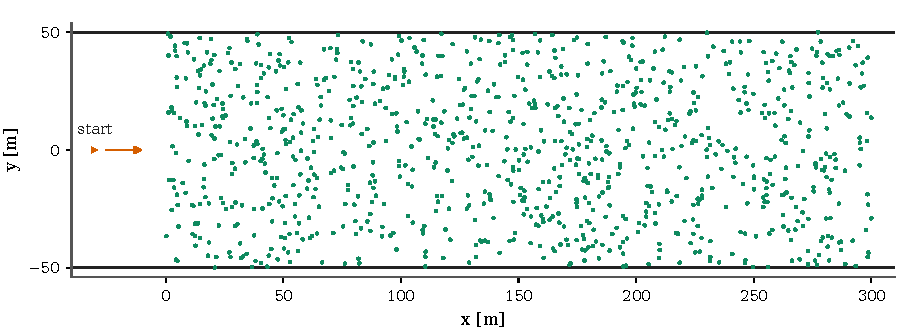
\includegraphics[width=\textwidth]{images/04_Simulation_Environment/forest_uniform.pdf}
\caption[A uniform density forest]{A uniform density forest seen from above: 975 trees placed independently and uniformly in a corridor of 300~m by 100~m. Trunks are drawn to scale. The thickets and the clearings are not designed: they are what independent positions look like.}
\label{fig:forest-uniform}
\end{figure}

A uniform forest is statistically the same at every point of the course, and this is what makes it useful for testing. It was used to verify the depth sensor and the collision test, to debug the flight of new bodies, and to observe how a controller behaves at one given density, without the confounding effect of a forest that changes as the drone advances.

The same property makes it a poor instrument for measuring. The difficulty of a uniform forest is a single number that has to be chosen in advance, and no choice suits a population of bodies of very different ability. In a sparse forest every competent body reaches the end and the progress saturates. In a dense forest every body fails within a few metres. Between these extremes the measure is dominated by chance. The cleanest way to see this is to consider a drone that flies straight and blind. Since the positions of the trees are independent, the risk of hitting one in the next metre is the same whatever the distance already flown. The distance covered before the collision therefore follows an exponential law, whose standard deviation equals its mean (\autoref{app:forest-math}). In the forest of \autoref{fig:forest-uniform}, with $b = 1.4$~m for the reference drone, that mean is 11~m, measured from the first tree. A controller that sees the trees does much better than this, but it inherits the structure of the problem. In a stationary forest the length of a flight has a large memoryless component, and many flights are needed before two bodies can be told apart.

\subsection{Growing Density Forests}
\label{subsec:forest-growing}

In the forests used for all the results of this thesis the density grows linearly along the course, from $\lambda_0$ trees per metre at the entrance to $\lambda_1$ at the end:
\begin{equation}
\lambda(x) = \lambda_0 + (\lambda_1 - \lambda_0)\,\frac{x}{L} .
\label{eq:forest-density}
\end{equation}
The number of trees is the integral of the profile, $N = \lceil (\lambda_0 + \lambda_1) L / 2 \rceil$. The lateral coordinate of each tree is uniform across the corridor, as before, and its coordinate along the course is drawn from the density \eqref{eq:forest-density} in closed form (\autoref{app:forest-math}). A whole batch of forests is thus generated with a handful of tensor operations. The entrance density $\lambda_0$ can also be drawn at random for each forest within a given range. This option is used during training, so that the controller meets dense forest at the beginning of a flight as well as at the end. \autoref{fig:forest-growing} shows one forest and its profile.

\begin{figure}[htbp]
\centering
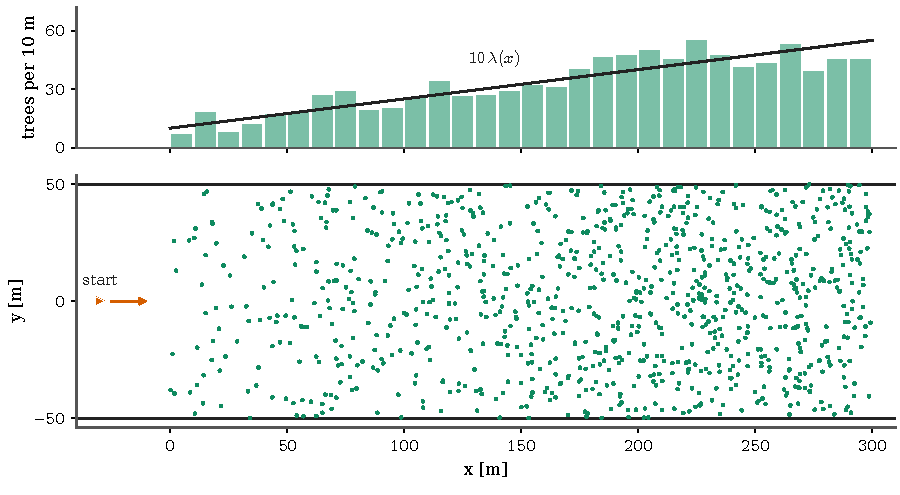
\includegraphics[width=\textwidth]{images/04_Simulation_Environment/forest_growing.pdf}
\caption[A growing density forest]{A growing density forest seen from above, with $\lambda_0 = 1$ and $\lambda_1 = 5.5$ trees per metre over 300~m, which gives the same number of trees, 975, as in \autoref{fig:forest-uniform}. The upper panel counts the trees in each 10~m of course and compares them with the profile \eqref{eq:forest-density}.}
\label{fig:forest-growing}
\end{figure}

The reason for this design is what it does to the measure. A growing forest is a course of increasing difficulty. Every flight, of whatever body, ends where the forest has become too dense for it, so the progress of a flight reads directly as the density that the pair of body and controller can cope with. A single course therefore orders the weak and the strong alike, the former in its first part and the latter in its last. As long as the course is long enough that nobody reaches its end, the measure does not saturate. The role of chance shrinks as well. For the blind straight flight, the risk of the next metre now grows with the distance already flown. Long flights become rapidly improbable instead of merely rare, and flights end in a band rather than anywhere (\autoref{app:forest-math}). In the forest of \autoref{fig:forest-growing} the blind flight covers 26~m on average from the first tree, and gets past 100~m less than once in a hundred attempts. Whatever a drone achieves beyond that is owed to what it sees and to how well its body lets it act on what it sees. That is exactly what the progress is meant to measure.

The design also helps learning. A controller at the beginning of its training crashes early and therefore only ever experiences the sparse part of the forest. As it improves, it reaches denser stretches, so the difficulty of its experience grows with its competence without any schedule having to be imposed. Finally, the positions remain independent. A growing forest thus keeps the irregular texture of the uniform one, with its thickets and its clearings, and this turned out to matter, as the next subsection explains.

\subsection{Latin Hypercube Forests}
\label{subsec:forest-latin}

Independent positions have a cost. Nothing prevents two trunks from being drawn on top of each other, or a few of them from lining up so closely that they form a wall. The effect is not marginal. For independent positions of areal density $n$, the probability that a tree has a neighbour closer than a distance $d$ is $1 - e^{-n\pi d^2}$. At one tree every 25~m$^2$, a density that the forests of this work reach in their last part, a quarter of the trunks overlap another trunk ($d = 2r$). Almost two thirds of them are separated from their nearest neighbour by a gap narrower than the width $b$ of the reference drone ($d = 2r + b$). Chains of such pairs form barriers several metres wide (\autoref{fig:forest-overlaps}, left). A flight that ends against one of them says little about the body or about the controller. This luck of the draw is one of the sources of the noise that every comparison in this thesis has to average out.

\begin{figure}[htbp]
\centering
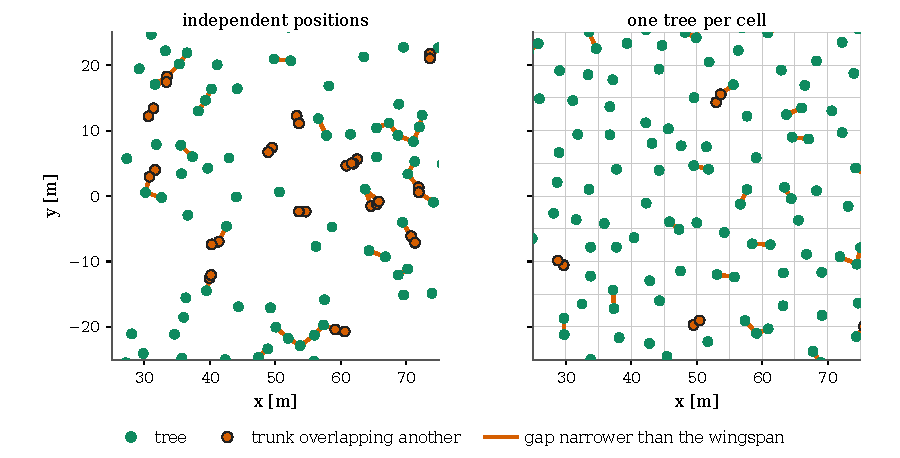
\includegraphics[width=\textwidth]{images/04_Simulation_Environment/forest_random_vs_stratified.pdf}
\caption[Independent and stratified positions at the same density]{Independent and stratified positions at the same density, one tree every 25~m$^2$, in a window of 50~m by 50~m with trunks to scale. With independent positions 25\% of the trunks overlap another and 64\% leave a gap narrower than the width $b = 1.4$~m of the reference drone; with one tree per cell the two figures fall to 6\% and 39\% (averages over 200 forests).}
\label{fig:forest-overlaps}
\end{figure}

The third generator was written to remove this effect. It borrows the idea of \emph{Latin hypercube sampling} \cite{mckay1979comparison}, the classical device for spreading random samples evenly over a domain: the domain is divided into strata, and the samples are forced to occupy the strata evenly while remaining random inside them. Here the corridor is tiled with rectangular cells, and exactly one tree is placed in each cell, at a position uniform within it. To keep the density growing along the course, the cells shrink. The course is cut into columns whose width decreases linearly from $s_0$ at the entrance to $s_1$ at the end, rescaled so that they tile the length $L$ exactly. Each column is then cut into equal rows whose height follows the same interpolation (\autoref{fig:forest-latin}). The name is used loosely. In a Latin hypercube proper each row and each column of the grid holds exactly one sample. Here every cell does, which is the stronger form of stratification also known as jittered sampling.

\begin{figure}[htbp]
\centering
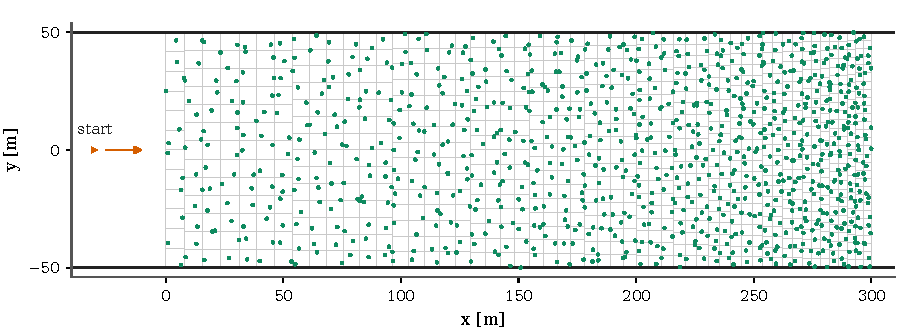
\includegraphics[width=\textwidth]{images/04_Simulation_Environment/forest_latin.pdf}
\caption[A Latin hypercube forest]{A Latin hypercube forest seen from above, with its cells. The cells shrink from 8~m to 3.4~m along the course and each holds exactly one tree, for 988 trees in total, about as many as in \autoref{fig:forest-uniform} and \autoref{fig:forest-growing}.}
\label{fig:forest-latin}
\end{figure}

The stratification does what it was meant to do. At the same density the overlapping trunks fall from 25\% to 6\%, and the gaps narrower than the width $b$ from 64\% to 39\% (\autoref{fig:forest-overlaps}, right). No region can be crowded, because at most four trees can meet around the corner shared by four cells. No region can be empty, because every cell is occupied. The number of trees is also identical in all the forests of a batch.

It was nevertheless abandoned, because what it removes is part of the task. A forest drawn in this way is tidy: the trees are almost evenly spaced and every gap is about one cell wide. The thickets and the clearings that a real forest has, and that \autoref{fig:forest-uniform} and \autoref{fig:forest-growing} show, are gone. A body and a controller selected in such a forest are selected in the presence of a regularity that no real environment offers, and a search could come to rely on it. Deciding when to go around a thicket and when to cut through a clearing is, on the contrary, part of what flying through a forest means. The choice made in this thesis is therefore to keep the forest natural and to pay for its luck with numbers. The results are obtained in growing density forests with independent positions, and the chance of an unlucky forest is averaged out over many of them.

\section{Drone Model}
\label{sec:drone-model}

The body that flies through the forest is a small electric aircraft with a morphing wing. It is not a fixed model. Every body is generated by a script that turns a genome of fifteen numbers into a URDF file, with its geometry, its masses and inertias, its joints and the reference frames of the aerodynamic solver of \autoref{subsec:genesis-aero}. All bodies share their architecture: the parts they are made of, how these parts are actuated and what the drone can sense. What distinguishes them is the size, the proportions and the placement of those parts. This section describes the common architecture first, then the genome, and finally the particular body that is used as the reference throughout the thesis.

\subsection{Drone Shape and Actuators}
\label{subsec:drone-shape}

The drone has a conventional layout (\autoref{fig:drone-actuators}). A straight fuselage of constant cross-section, 10~cm wide, carries a propeller of 10~cm radius at its nose, a wing made of two independent rectangular panels attached to its sides, and a tail at its rear end. The tail is formed by a horizontal surface, the elevator, and a vertical one, the rudder. The fuselage also houses the battery, the electronics and a small camera at the nose, which are fixed masses.

What is not conventional is the way the drone is controlled. There are no ailerons, no flaps and no hinged control surfaces of any kind: the surfaces move as a whole. Each wing panel is connected to the fuselage by two revolute joints in series, which share the same point at its root, on the quarter-chord line. The first joint rotates the panel about the vertical axis and changes its \emph{sweep}. The second rotates it about its own spanwise axis and changes its \emph{twist}, that is, its incidence. The elevator is a single all-moving surface that pitches about a hinge at the end of the fuselage. The rudder is an all-moving fin that turns about a vertical axis mounted on the elevator, so that it pitches with it. Together with the throttle of the propeller, this gives the seven commands that a controller issues at every control step:
\begin{equation}
\vect{a} = \left( u,\; \delta^{\mathrm{sw}}_{\mathrm{L}},\; \delta^{\mathrm{sw}}_{\mathrm{R}},\; \delta^{\mathrm{tw}}_{\mathrm{L}},\; \delta^{\mathrm{tw}}_{\mathrm{R}},\; \delta^{\mathrm{el}},\; \delta^{\mathrm{ru}} \right),
\label{eq:drone-actions}
\end{equation}
the throttle $u \in [0,1]$ and six target angles, each bounded by the mechanical range of its joint. The two panels are commanded independently. The wing can therefore be moved symmetrically, to trim the aircraft and to change its lift, or asymmetrically, to roll and to turn: a differential twist does the work of the ailerons of a conventional aircraft. This is the kind of morphing wing studied for winged drones by Bergonti et al. \cite{bergonti2024codesign}, here combined with a moving tail.

\begin{figure}[htbp]
\centering
\begin{subfigure}[c]{0.44\textwidth}
\centering
\begin{tikzpicture}[>={Stealth[length=2mm]}, thick, scale=0.92, transform shape, every node/.style={font=\scriptsize}]
\tikzset{
  part/.style={draw=black!65, fill=black!8, rounded corners=1.5pt},
  joint/.style={draw=orange!60!black, fill=orange!35, circle, inner sep=0pt, minimum size=5pt},
  tag/.style={draw=orange!60!black, fill=orange!14, rounded corners=1.5pt, inner sep=2.2pt, align=center},
}
% fuselage, propeller
\draw[part] (-0.22,-2.2) rectangle (0.22,2.0);
\draw[part, fill=black!55] (-0.85,2.06) rectangle (0.85,2.2);
\draw[->, orange!60!black, very thick] (0,2.3) -- (0,2.95);
\node[tag, anchor=west] at (0.3,2.72) {throttle $u$};
% wing panels
\draw[part] (-2.95,0.55) rectangle (-0.42,1.25);
\draw[part] (0.42,0.55) rectangle (2.95,1.25);
\node[joint] at (-0.32,1.07) {};
\node[joint] at (0.32,1.07) {};
\node[tag] at (-1.7,0.05) {sweep $\delta^{\mathrm{sw}}_{\mathrm{L}}$, twist $\delta^{\mathrm{tw}}_{\mathrm{L}}$};
\node[tag] at (1.7,0.05) {sweep $\delta^{\mathrm{sw}}_{\mathrm{R}}$, twist $\delta^{\mathrm{tw}}_{\mathrm{R}}$};
% tail
\draw[part] (-1.25,-2.75) rectangle (1.25,-2.33);
\draw[part, fill=black!30] (-0.06,-2.95) rectangle (0.06,-2.25);
\node[joint] at (0,-2.27) {};
\node[tag, anchor=west] at (0.45,-1.75) {elevator $\delta^{\mathrm{el}}$, rudder $\delta^{\mathrm{ru}}$};
\end{tikzpicture}
\caption{}
\label{fig:drone-actuators-scheme}
\end{subfigure}
\hfill
\begin{subfigure}[c]{0.54\textwidth}
\centering
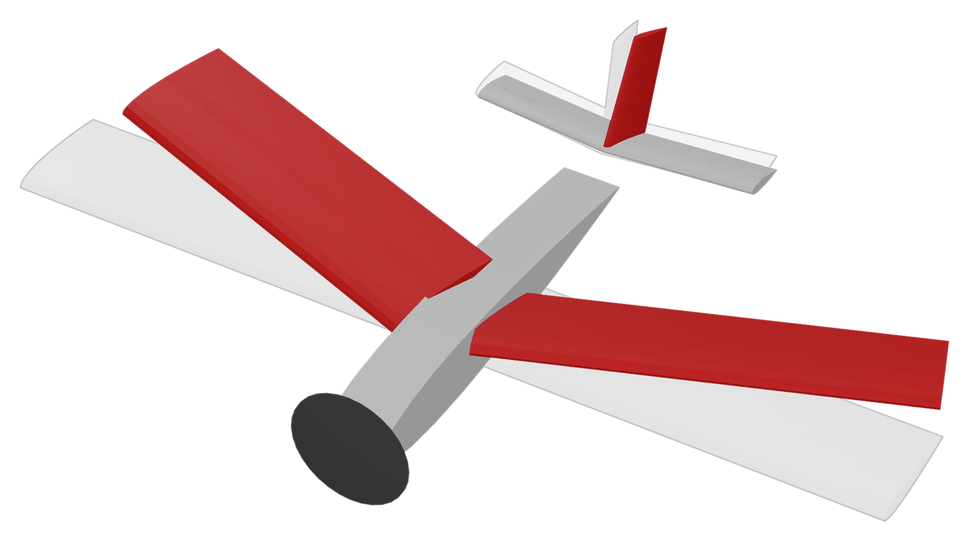
\includegraphics[width=\textwidth]{images/04_Simulation_Environment/standard_drone_actuation.png}
\caption{}
\label{fig:drone-actuators-render}
\end{subfigure}
\caption[Parts and actuators of the drone]{Parts and actuators of the drone. (a) The seven commands, on a schematic top view with the nose up: the throttle of the propeller, the sweep and the twist of each wing panel, the elevator and the rudder. (b) The reference drone with the left panel swept back to the limit of its range, the two panels twisted in opposite directions, and the elevator and the rudder deflected; the neutral position of every surface is shown in light grey.}
\label{fig:drone-actuators}
\end{figure}

\paragraph{Servomotors and gear ratios.} Every joint is driven by a servomotor, modelled as in \autoref{subsec:genesis-physics}: a position controller with a bounded torque, acting against the damping and the friction of the joint. The sweep joints use a larger servomotor than the twist and the tail joints (25~g against 10~g). Between the servomotor and a wing joint there is a reduction gear whose ratio $k$ is part of the genome: one ratio for the sweep of both panels and one for their twist. A gear trades range for strength. The panel can move within
\begin{equation}
\lvert \delta^{\mathrm{sw}} \rvert \le \frac{0.7}{k_{\mathrm{sw}}}~\text{rad}, \qquad \lvert \delta^{\mathrm{tw}} \rvert \le \frac{0.5}{k_{\mathrm{tw}}}~\text{rad},
\label{eq:drone-gear}
\end{equation}
with a torque limit of $0.75\, k_{\mathrm{sw}}$ and $0.6\, k_{\mathrm{tw}}$~N\,m respectively, while the damping and the friction felt at the joint grow with $k^2$ and with $k$. With the ratios allowed by the genome, between 1.5 and 3.5, the sweep range goes from $\pm 27^{\circ}$ to $\pm 11^{\circ}$ and the twist range from $\pm 19^{\circ}$ to $\pm 8^{\circ}$. A body can thus have a wing that moves widely but weakly, or narrowly but firmly. Which of the two is better depends on the aerodynamic loads that its panels generate, that is, on the rest of the body. The tail joints have no gear: their range is $\pm 0.25$~rad ($\pm 14^{\circ}$) and their torque limit 1~N\,m on every body. The controller never commands an angle directly. Its six outputs lie in $[-1, 1]$ and are scaled by the range of the corresponding joint, so that the same output means ``full deflection'' on every body.

\paragraph{Masses.} The structure is foam, and each part receives the mass of its volume and the inertia tensor of a box of its dimensions. Fixed masses are added for the battery and the electronics, the camera, the motor and the propeller, the six servomotors, and the hinges and fittings. The fixed masses amount to about 0.40~kg and are the same for every body; the structural mass is what the genome controls. It grows quickly with the size of the wing, since the volume of a panel is proportional to the cube of its span for a given aspect ratio and section. The lightest body that the genome can express weighs 0.44~kg and the heaviest 2.5~kg, while nine bodies out of ten drawn uniformly at random weigh between 0.50 and 1.10~kg. The position of the centre of mass is controlled by a gene as well, which places the mass of the fuselage, battery included, along its length. The densities and the fixed masses are listed in \autoref{app:drone-mass-power}.

\paragraph{Energy.} The second quantity by which a body is evaluated, next to the progress of \autoref{sec:flight-environment}, is the energy it spends. The power absorbed by the propeller follows from its rotation speed and its advance ratio, with the same kind of law as the thrust (\autoref{app:drone-mass-power}); at full throttle with the drone at rest it is about 83~W. Each servomotor absorbs the mechanical power it delivers plus a resistive loss proportional to the square of its torque, and never less than zero, since a servomotor that is driven backwards by the air does not recharge the battery. Holding a panel against a steady aerodynamic load therefore costs energy even when nothing moves. No other consumption is modelled, and the losses of the motor and of its speed controller are neglected. The energy $E$ of a flight is the integral of the total power up to the end of the flight. It is compared across bodies of different weight through the dimensionless \emph{cost of transport},
\begin{equation}
\mathit{CoT} = \frac{E}{m\, g\, \Delta x},
\label{eq:drone-cot}
\end{equation}
where $m$ is the nominal mass of the body, $g$ the acceleration of gravity and $\Delta x$ the progress of the flight: the energy spent to carry one unit of weight over one unit of distance along the corridor. Distance flown sideways or in circles adds to the energy and not to the progress, so a body that needs wide manoeuvres to get through the trees pays for them.

\subsection{Sensors}
\label{subsec:drone-sensors}

Every body carries the same sensors, and their readings are the only information about the world that a controller receives. \autoref{tab:drone-sensors} lists them. The drone knows its altitude, its attitude and its velocity, and it has a depth sensor that looks ahead. It does not know where it is along or across the corridor. It has no measure of its angular rates, of its airspeed or of the angles of its own joints, and no sensor tells it which body it is flying. The measurements are delivered at the control rate of 25~Hz, and each is corrupted by Gaussian noise, as anticipated in \autoref{subsec:genesis-noise}. Besides the measurements, the controller receives two quantities that are not sensed: the seven commands it issued at the previous step, and the forward speed it is asked to keep.

\begin{table}[htbp]
\centering
\begin{tabularx}{\textwidth}{>{\raggedright\arraybackslash}X c >{\raggedright\arraybackslash}X}
\hline
Quantity & Size & Noise (standard deviation) \\
\hline
Altitude above the ground & 1 & 0.1~m \\
Attitude, as a unit quaternion & 4 & 0.01 on each component \\
Linear velocity in the world frame & 3 & 0.4~m/s along the corridor, 0.2~m/s on the other axes \\
Depth ahead, one value per sector & 20 & 1.5~m \\
\hline
Commands issued at the previous step & 7 & none \\
Commanded forward speed & 1 & none \\
\hline
\end{tabularx}
\caption[Sensors of the drone]{What the controller receives at every control step: 28 measurements, with the noise added to each, and 8 quantities that are not measured, for 36 numbers in total.}
\label{tab:drone-sensors}
\end{table}

\paragraph{Depth sensor.} The depth sensor is what lets the drone see the forest. It looks forward in the horizontal plane. A fan of $80^{\circ}$ centred on the heading is divided into 20 equal sectors. Each sector reports the distance to the surface of the nearest trunk that falls inside it, even partially, or to the lateral wall of the corridor if that is closer, up to a range of 30~m (\autoref{fig:forest-sensing}). When the drone banks, the fan narrows by the cosine of the roll angle, as the horizontal footprint of a sensor fixed to the body would. The result is a one-dimensional depth image of 20 pixels, a deliberately poor sensor. It has no vertical resolution, its range is about two seconds of flight, and a trunk hidden behind another is invisible until the first has been passed. The sensor is one of the custom kernels mentioned in \autoref{subsec:genesis-proscons}, and it runs for all environments at once.

\begin{figure}[htbp]
\centering
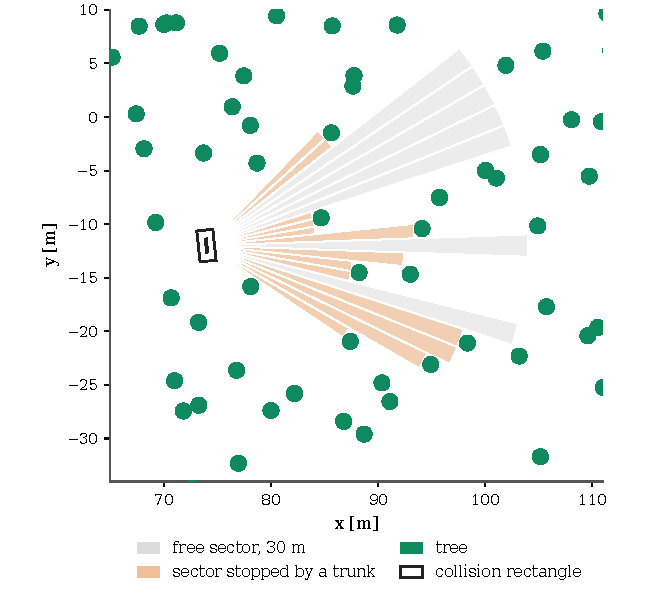
\includegraphics[width=0.74\textwidth]{images/04_Simulation_Environment/forest_sensing.pdf}
\caption[Depth sectors and collision rectangle]{What the forest is to the drone, seen from above. The depth sensor divides a fan of $80^{\circ}$ ahead of the drone into 20 sectors and reports for each the distance to the nearest trunk, up to 30~m. The collision test of \autoref{sec:flight-environment} asks whether the centre of a trunk lies inside the rectangle drawn around the wing (trunks and wingspan are to scale).}
\label{fig:forest-sensing}
\end{figure}

\subsection{Drone Genome}
\label{subsec:drone-genome}

A body is a point in a space of fifteen parameters, its \emph{genome} (\autoref{tab:drone-genome}). Each gene is stored as a number in $[0,1]$, the form in which the evolutionary algorithms handle it, and is mapped linearly onto the physical range of its parameter when the body is built. Twelve genes are continuous. The remaining three select the wing section among the four-digit NACA airfoils and are discrete: the unit interval is divided into as many equal bins as there are admissible values, and the gene takes the value of the bin it falls in.

\begin{table}[htbp]
\centering
\begin{tabularx}{\textwidth}{r >{\raggedright\arraybackslash}X c c}
\hline
 & Gene & Range & Reference drone \\
\hline
1 & Span of one wing panel & 0.4 to 0.9~m & 0.7~m \\
2 & Aspect ratio of one wing panel (span over chord) & 1.5 to 5 & 3.5 \\
3 & Length of the fuselage & 0.4 to 0.9~m & 0.73~m \\
4 & Position of the mass of the fuselage, as a fraction of its length from the nose & 0.30 to 0.60 & 0.38 \\
5 & Position of the wing root, as a fraction of the fuselage length from the nose & 0.30 to 0.60 & 0.38 \\
6 & Span of the elevator & 0.2 to 0.6~m & 0.5~m \\
7 & Aspect ratio of the elevator & 1.5 to 4 & 4 \\
8 & Span of the rudder & 0.1 to 0.4~m & 0.2~m \\
9 & Aspect ratio of the rudder & 1.5 to 4 & 2 \\
10 & Dihedral angle of the wing panels & $-4^{\circ}$ to $4^{\circ}$ & $0^{\circ}$ \\
11 & Gear ratio of the sweep joints & 1.5 to 3.5 & 2 \\
12 & Gear ratio of the twist joints & 1.5 to 3.5 & 2.5 \\
13 & Airfoil: maximum camber (first NACA digit) & 0 to 4 & 3 \\
14 & Airfoil: position of the maximum camber (second digit) & 2 to 5 & 4 \\
15 & Airfoil: thickness (last two digits) & 10 to 20 & 16 \\
\hline
\end{tabularx}
\caption[Genome of the drone]{The genome of the drone: fifteen genes, their physical ranges, and the values of the reference drone of \autoref{subsec:drone-standard}. The last three genes are discrete.}
\label{tab:drone-genome}
\end{table}

The first two genes define the wing. Its panels are rectangular, and the genes give the span $b_p$ of one panel and its aspect ratio, from which the chord is $\bar c = b_p / \mathit{AR}_p$. The two panels are mounted on the sides of a fuselage of width $w_f = 0.1$~m. The wing as a whole therefore has a span of $2 b_p + w_f$ from tip to tip, between 0.9 and 1.9~m, and an aspect ratio of $(2 b_p + w_f)/\bar c$. This is the aspect ratio that enters the aerodynamic model (\autoref{subsec:genesis-aero}), and for the reference drone it is 7.5. The same construction holds for the elevator, whose gene is its total span, while the rudder is a single panel. Genes 3 to 5 lay the aircraft out along its axis. The length of the fuselage sets the lever arm of the tail, which sits at its end. The positions of the wing and of the mass of the fuselage along it decide, together, how far the centre of mass lies from the point where the lift of the wing acts. This distance governs the longitudinal stability of an aircraft, and a small change of either gene can turn a docile body into one that is hard or impossible to control. The dihedral gene tilts the two panels upwards or downwards at their root. The two gear ratios set the authority of the morphing wing, as described above.

The airfoil genes act in two ways. The thickness of the section is the thickness of the panel, and therefore changes its mass and its inertia. And the section as a whole selects a row in the table of airfoil parameters of \autoref{subsec:genesis-aero}, from which the aerodynamic solver reads the zero-lift angle, the stall angle, the parasitic drag and the nominal Reynolds number of the wing. The tail surfaces are not part of the genome in this respect: they always use the same symmetric section, 16\% thick.

No constraint is imposed on the genome beyond its ranges. The generator does not check that a body is well proportioned, that its wing and its tail do not interfere, or that it is stable. Any point of the unit hypercube becomes a body, and whether that body can fly is left for the flights to decide. The ranges were chosen so that a large part of the space is flyable, but nothing prevents the search from visiting the rest.

\subsection{The Standard Drone}
\label{subsec:drone-standard}

One body is singled out as the reference of the whole thesis (\autoref{fig:drone-standard}). It is the body against which the evolved ones are compared, and the point from which the quantities of this chapter were illustrated. Its genome is the last column of \autoref{tab:drone-genome}. Its wing measures 1.5~m from tip to tip, with a chord of 0.2~m and a NACA 3416 section. Its fuselage is 0.73~m long, for an overall length of 0.89~m, and it weighs 0.605~kg.

\begin{figure}[htbp]
\centering
\begin{subfigure}[c]{0.52\textwidth}
\centering
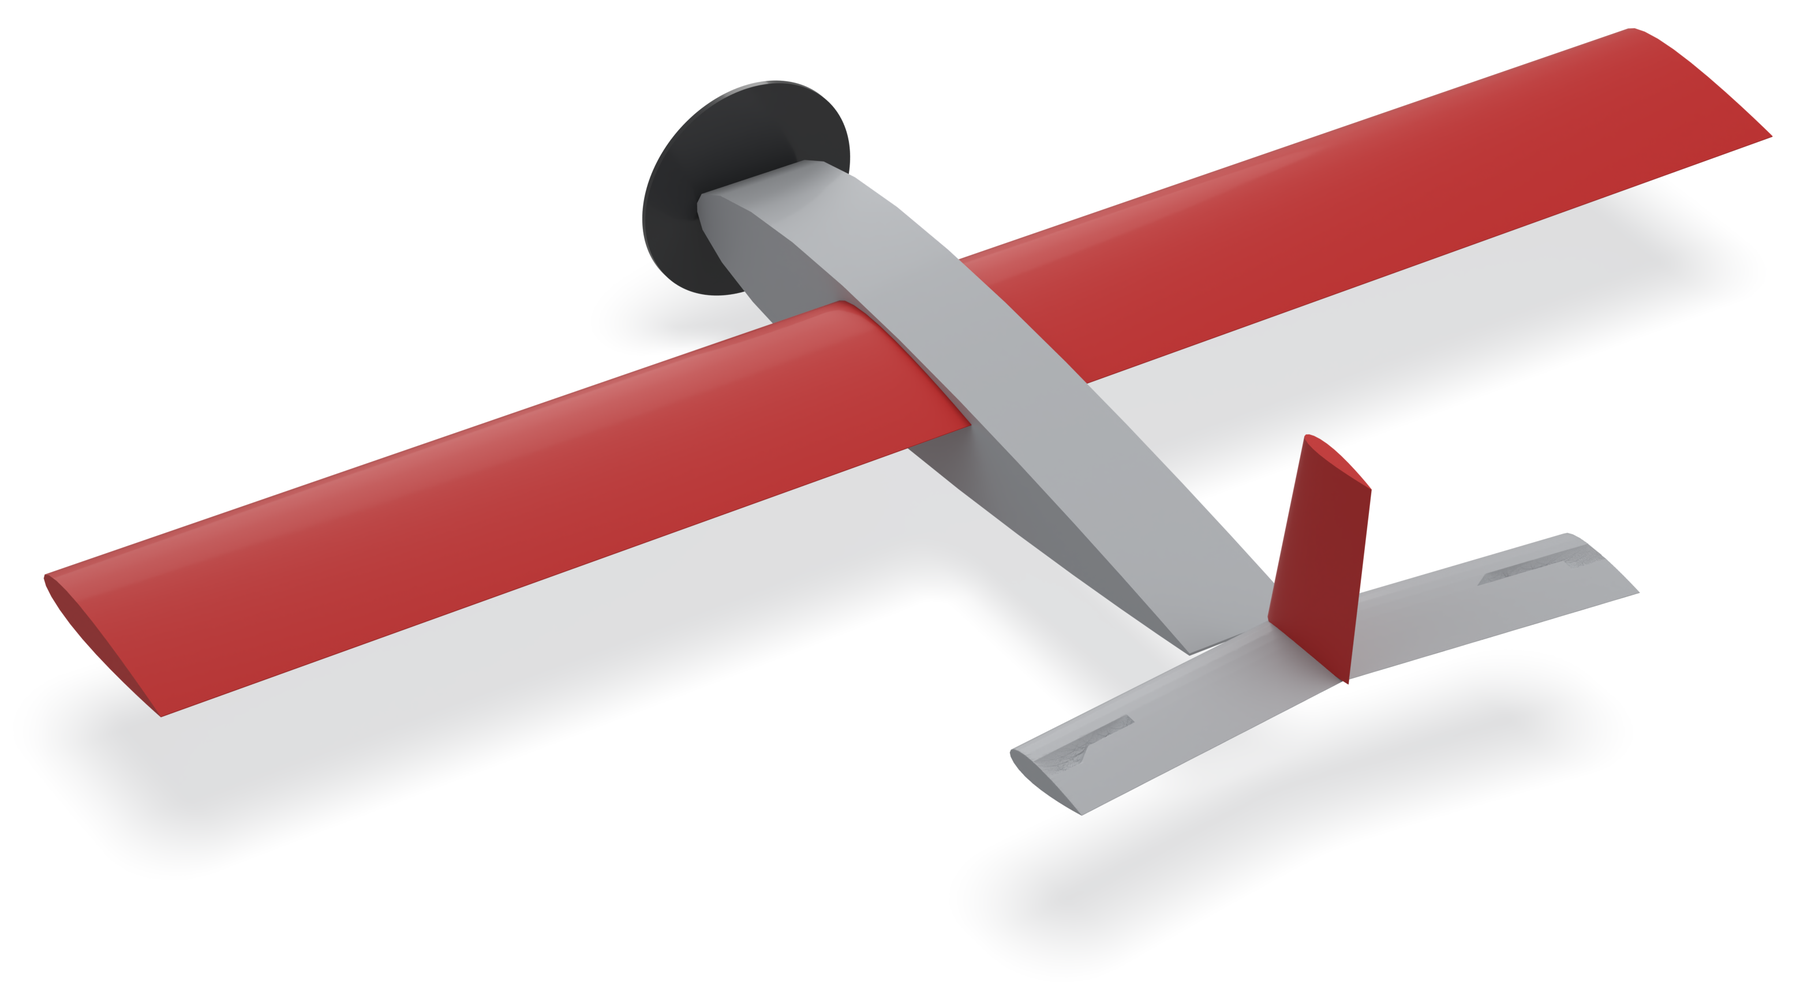
\includegraphics[width=\textwidth]{images/04_Simulation_Environment/standard_drone_neutral_3quarter.png}
\caption{}
\end{subfigure}
\hfill
\begin{subfigure}[c]{0.44\textwidth}
\centering
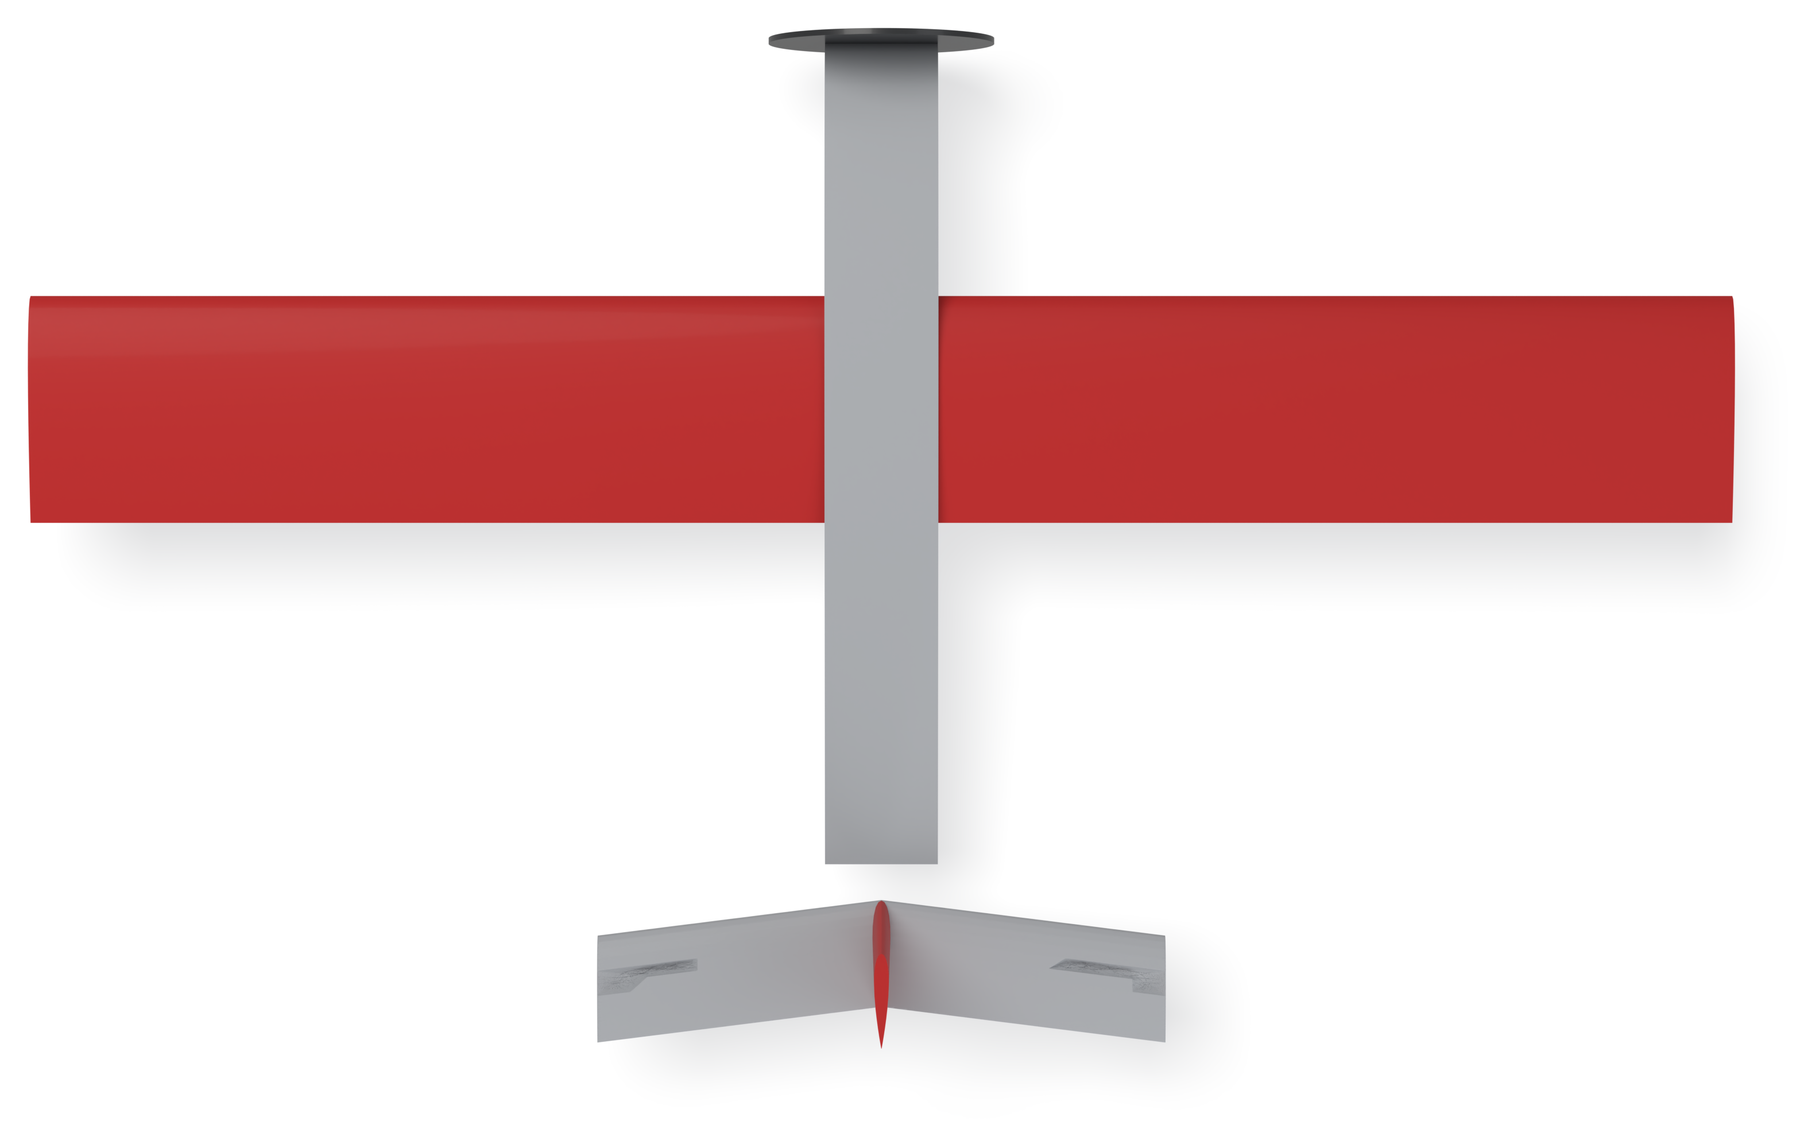
\includegraphics[width=\textwidth]{images/04_Simulation_Environment/standard_drone_neutral_top.png}
\caption{}
\end{subfigure}
\caption[The standard drone]{The standard drone with all joints in their neutral position: (a) three-quarter view, (b) top view with the nose up. The wing panels and the rudder are drawn in red, the fuselage and the elevator in grey, the disc of the propeller in black.}
\label{fig:drone-standard}
\end{figure}

These numbers are not arbitrary. The dimensions of the standard drone and the section of its wing are those of the H-King Bixler~3 \cite{hobbyking2026bixler3}, a commercial foam glider with a wingspan of 1.55~m and a length of 0.95~m. The Bixler~3 is widely used as a research platform, and Bergonti et al. \cite{bergonti2024codesign} adopt it as the baseline of their co-design study. For this reason the figures of this thesis label the standard drone with the name of that aircraft. The correspondence, however, stops at the geometry. The Bixler~3 is flown with ailerons, an elevator and a rudder hinged on fixed surfaces, and is pushed by a propeller mounted behind its wing. The standard drone has none of those control surfaces: it steers by sweeping and twisting its wing panels and by moving its tail surfaces as a whole, and it is pulled by a propeller at its nose. It is also lighter, since the commercial aircraft weighs 0.89~kg ready to fly. The two aircraft share a shape, not a set of actuators, and their flight dynamics are therefore not directly comparable. The standard drone should be read as a body of familiar proportions inside the design space of \autoref{tab:drone-genome}, not as a model of the commercial aircraft.

\chapter{Methodology}
\label{ch:method}

\autoref{ch:challenges} ended with the shape that any workable answer must have: a controller that is paid for once, for the whole space of bodies, and an adaptation to the body being scored that costs no more than the flights that score it. This chapter describes the method that gives that shape a content, in the order in which the method is built. \autoref{sec:base-controllers} trains by reinforcement learning the controllers on which everything else rests. \autoref{sec:hebbian-controller} takes one of them, freezes it, and makes its output layer plastic through Hebbian rules. \autoref{sec:pipeline} describes the co-design pipeline, in which an inner loop evolves those rules and an outer loop evolves the bodies they are meant to serve, and whose results are reported in \autoref{ch:results}.

\section{Base Controllers}
\label{sec:base-controllers}

Everything in the method rests on a controller that can already fly. Two kinds of such controllers are used in this thesis. They share the architecture, the task, the reward and the learning algorithm, and differ only in the bodies they are trained on. A \emph{generalist} is trained on a large pool of different bodies at once: it is the $\vect{\theta}_G$ of \autoref{sec:challenge-morphology}, a single set of weights that is expected to fly any body of the design space, and it is the controller on which the co-design loop is built. A \emph{specialist} is trained on one body alone: it is the closest that this thesis comes to the $\vect{\theta}^{\star}(\vect{m})$ of \eqref{eq:codesign-bilevel}, and it serves as a term of comparison and as a second base on which the rules of \autoref{sec:hebbian-controller} are evolved. Both are trained with PPO (\autoref{subsec:ppo}), in the implementation of the RSL-RL library \cite{rudin2022learning}, which was written for the regime used here: thousands of environments simulated in parallel on the GPU, each contributing a short segment of experience to every update. This section describes the network first, then the environment in which it is trained and the reward that defines what flying well means, and finally the two training regimes with their numbers.

\subsection{Architecture of the Controller}
\label{subsec:controller-architecture}

The controller is the actor of an actor-critic pair (\autoref{subsec:actor-critic}). At every control step, 25 times per second, it receives the 36 numbers of \autoref{tab:drone-sensors}, collected in the observation $\vect{o}_t$, and returns the seven commands $\vect{a}_t$ of \eqref{eq:drone-actions}. Before entering the network each component of the observation is standardized with the running mean and standard deviation of the observations collected during training; these statistics are frozen after the first $10^8$ samples, about a hundred iterations, and are stored with the weights. The network itself is small (\autoref{fig:controller-architecture}): an LSTM layer of 128 units (\autoref{sec:lstm}), two fully connected layers of 128 and 32 units with the exponential linear unit (ELU) as activation \cite{clevert2016elu}, and a linear output layer of seven units.

\begin{figure}[htbp]
\centering
\begin{tikzpicture}[>={Stealth[length=2mm]}, thick, scale=0.9, transform shape, every node/.style={font=\small}]
\tikzset{
  alayer/.style={draw=orange!70!black, fill=orange!12, rounded corners, thick, align=center, minimum width=1.55cm, minimum height=1.05cm},
  aplastic/.style={alayer, very thick, fill=orange!40},
  clayer/.style={draw=violet!60!black, fill=violet!10, rounded corners, thick, align=center, minimum width=1.55cm, minimum height=1.05cm},
}
% ---- actor
\node[align=center] (o) at (0,0) {observation\\$\vect{o}_t$ (36)};
\node[alayer] (al) at (2.7,0) {LSTM\\128};
\node[alayer] (a1) at (4.8,0) {128\\ELU};
\node[alayer] (a2) at (6.9,0) {32\\ELU};
\node[aplastic] (a3) at (9.1,0) {linear\\$32 \to 7$};
\node[tanhbox, align=center] (as) at (11.5,0) {sample,\\$\tanh$};
\node[align=center] (a) at (14.0,0) {commands\\$\vect{a}_t$ (7)};
\draw[->] (o) -- (al);
\draw[->] (al) -- (a1);
\draw[->] (a1) -- (a2);
\draw[->] (a2) -- node[above]{\scriptsize $\vect{x}_t$} (a3);
\draw[->] (a3) -- node[above]{\scriptsize $\vect{\mu}_t$} (as);
\draw[->] (as) -- (a);
\draw[->] (al.north east) .. controls +(0.55,0.95) and +(-0.55,0.95) .. node[above]{\scriptsize $\vect{h}_{t-1}, \vect{c}_{t-1}$} (al.north west);
\node[font=\scriptsize, text=orange!45!black] at (9.1,-0.85) {224 weights};
\node[font=\scriptsize, text=red!50!black] at (11.5,-0.85) {$\vect{\sigma}$ learned};
\node[anchor=east, font=\scriptsize, text=gray!50!black] at (15.0,1.3) {actor: trained, then deployed};
% ---- critic
\node[align=center] (po) at (0,-3.2) {privileged\\observation (67)};
\node[clayer] (cl) at (2.7,-3.2) {LSTM\\128};
\node[clayer] (c1) at (4.8,-3.2) {128\\ELU};
\node[clayer] (c2) at (6.9,-3.2) {128\\ELU};
\node[clayer] (c3) at (9.1,-3.2) {linear\\$128 \to 1$};
\node[align=center] (v) at (11.5,-3.2) {value\\$V_{\vect{w}}$};
\draw[->] (po) -- (cl);
\draw[->] (cl) -- (c1);
\draw[->] (c1) -- (c2);
\draw[->] (c2) -- (c3);
\draw[->] (c3) -- (v);
\draw[->] (cl.north east) .. controls +(0.55,0.95) and +(-0.55,0.95) .. (cl.north west);
\node[anchor=east, font=\scriptsize, text=gray!50!black] at (15.0,-1.9) {critic: used during training only};
\end{tikzpicture}
\caption[The networks of a base controller]{The two networks of a base controller, with the sizes of the generalist. The actor maps the observation of \autoref{tab:drone-sensors} to the seven commands; its output layer, highlighted, is the part of the network on which the rest of the method acts. The critic estimates the value of the current state from a richer input, which for the generalist includes the genome of the body (the critic of a specialist does without it and has 52 inputs), and is discarded when training ends.}
\label{fig:controller-architecture}
\end{figure}

The recurrent layer comes first, and its role is to make the controller stateful. The task is only partially observable: the drone does not measure its angular rates, its airspeed or the angles of its joints (\autoref{subsec:drone-sensors}); its measurements are noisy; and its commands take effect after a latency that changes from flight to flight, through servomotors that respond with a delay of their own. A controller without memory would have to decide from a single noisy snapshot of all this. A controller with a state can use the history of what it observed and commanded: a rate from successive attitudes, the state of an actuator from the commands that were sent to it, a measurement steadied by those that preceded it. This is why the previous commands are part of the observation, and why the memory is placed where it acts on the raw history.

The two fully connected layers compress the state of the LSTM into a vector $\vect{x}_t \in \mathbb{R}^{32}$, from which the output layer computes
\begin{equation}
\vect{\mu}_t = \mat{W}\, \vect{x}_t + \vect{b}, \qquad \mat{W} \in \mathbb{R}^{7 \times 32}.
\label{eq:actor-output}
\end{equation}
The width of the last hidden layer fixes the size of the output layer at $7 \times 32 = 224$ weights, a number that matters later: the output layer is the part of the controller that \autoref{sec:hebbian-controller} makes plastic, and every one of its weights will carry evolved coefficients. In total the actor has 105\,863 weights and biases, four fifths of which belong to the LSTM.

The policy is stochastic. The output $\vect{\mu}_t$ is the mean of a Gaussian from which a vector is sampled and then squashed,
\begin{equation}
\vect{z}_t \sim \mathcal{N}\!\big(\vect{\mu}_t,\, \operatorname{diag}(\vect{\sigma}^2)\big), \qquad \tilde{\vect{a}}_t = \tanh(\vect{z}_t) \in (-1, 1)^7,
\label{eq:actor-sampling}
\end{equation}
where $\vect{\sigma}$ is a vector of seven learned parameters that does not depend on the observation, initialized at 0.3. The first component of $\tilde{\vect{a}}_t$ becomes the throttle, $u = (\tilde{a}_1 + 1)/2$, and each of the other six is multiplied by the range of its joint \eqref{eq:drone-gear} to give a target angle. The squashing keeps every command inside its range by construction. The usual alternative, a Gaussian whose samples are clipped at the limits, makes the executed command differ from the sampled one whenever a limit is hit, and the probability ratio on which PPO relies is then computed for an action that was not the one taken. With \eqref{eq:actor-sampling} the density of the executed command is known exactly: it is the Gaussian density of $\vect{z}_t$ corrected by the Jacobian of the hyperbolic tangent \cite{haarnoja2018soft}.

One input is absent on purpose: the actor never receives the genome of the body, nor any other description of it, whether it is trained on one body or on many. The controller does not know which body it is flying. The purpose is to let it learn to fly any morphology without hints on what its flight dynamics could be. This is the opposite of the choice made by MetaMorph \cite{gupta2022metamorph}, whose policy reads a description of its morphology. A generalist trained in this way is one set of weights for all bodies and is adapted to none of them in particular; adapting it to the body it is given is the task of the next section.

The critic has no such restriction, because it is never deployed. It is a separate network with its own LSTM layer of 128 units, two fully connected layers of 128 units and a scalar output, and it is an asymmetric critic \cite{pinto2018asymmetric}. Its input has 67 components: the 36 of the actor, but without sensor noise; the angular velocity of the fuselage, the angles and the rates of the six joints, and the thrust actually delivered by the propeller, as a fraction of its maximum; and the 15 genes of the body. The value of a state depends on the body that is in it, since the same attitude and the same trees ahead promise more to a body that turns readily than to one that does not, and the critic can simply be told what the actor is never told. The genome shown to the critic is perturbed by Gaussian noise, with a standard deviation of 10\% of the range of each gene drawn once per flight and of 2\% drawn at every step (the discrete airfoil genes excepted), so that it reads as a description of a body rather than as the label of one of the training bodies.

\subsection{Training Environment}
\label{subsec:training-environment}

The controllers are trained on the task of \autoref{sec:flight-environment}, with the simulation noise and the sensors described in the same chapter. What that chapter left open are the numbers, which \autoref{tab:training-environment} collects.

\begin{table}[htbp]
\centering
\begin{tabularx}{\textwidth}{>{\raggedright\arraybackslash}p{4.6cm} >{\raggedright\arraybackslash}X}
\hline
Quantity & Value during training \\
\hline
Course & growing density forest (\autoref{subsec:forest-growing}), 150~m long and 100~m wide \\
Density at the end, $\lambda_1$ & 4 trees per metre \\
Density at the entrance, $\lambda_0$ & uniform between 0 and 3 trees per metre, drawn for each forest \\
Forests & ten for each environment, generated once; one of them drawn at random at every flight \\
Commanded speed & uniform between 5 and 25~m/s, drawn at every flight and held \\
Release point & $(-30, 0, 15)$~m, displaced uniformly by up to $\pm 15$~m along the course, $\pm 40$~m across it and between $-10$ and $+5$~m in altitude \\
Initial velocity & forward component uniform between 5 and 25~m/s; lateral and vertical components normal, with a standard deviation of 1~m/s; nose aligned with the velocity \\
End of a flight & as in \autoref{sec:flight-environment}: the ground is an altitude of 0.1~m, the collision margin is 0.2~m, the attitude limits are $90^{\circ}$ and the time limit is 100~s (2\,500 control steps) \\
Latency of the commands & zero or one control step, drawn at every flight \\
Offset of the joint targets & normal, with a standard deviation of 0.01~rad drawn at every flight plus 0.005~rad drawn at every step \\
\hline
\end{tabularx}
\caption[The training environment in numbers]{The training environment in numbers. Sensor noise is that of \autoref{tab:drone-sensors}; the aerodynamic noise and the randomization of masses and centres of mass are those of \autoref{subsec:genesis-noise}.}
\label{tab:training-environment}
\end{table}

The course is short, 150~m, and dense from the start. With an entrance density drawn between 0 and 3 trees per metre a forest holds between 300 and 525 trees, and the controller meets, in the first metres of some flights, the density that other flights reach only at the end: this is the option anticipated in \autoref{subsec:forest-growing}, and it prevents the first part of every flight from being an empty stretch in which nothing is learned about trees. A flight that ends is replaced at once, in the same environment, by a new one with a new forest, a new commanded speed and a new release.

The release is randomized for two reasons. The environments all begin together, and without it their first seconds would be thousands of copies of the same flight. And a controller that is always released in trimmed flight on the axis of the corridor never learns to recover: here it starts anywhere across the corridor, as low as 5~m above the ground, and at a speed that has nothing to do with the one it is asked to keep, so that the first thing it has to do in every flight is accelerate or slow down. The range of the commands is wider than what most bodies can hold: the reference drone stalls below about 6~m/s, and above 23~m/s the propeller of \eqref{eq:prop-thrust} delivers no thrust to any body. A command near either end cannot be met in level flight, and the tracking term of the reward then favours the closest speed that the body can reach; the evaluations of the following sections use a narrower range of commands. The commanded speed makes of the controller a family of controllers indexed by one number. Both quantities by which flights are judged depend on the speed, since a faster flight leaves less time to react to a trunk that appears at 30~m and changes the energy spent per metre, and leaving the speed as an input keeps that choice open instead of burying it in the weights. The evaluations of the following sections exploit it by flying every body over a range of commanded speeds.

\subsection{Reward Function}
\label{subsec:reward}

In this thesis the bodies are piloted by the Hebbian controllers of \autoref{sec:hebbian-controller} and judged by two quantities, the progress and the cost of transport \eqref{eq:drone-cot}, which are properties of a whole flight. They say nothing about which of the hundreds of commands of a flight were good ones, and a learning signal is needed at every step. The reward is therefore a separate object, designed to be informative step by step and to have, as its maximizer, a pilot that does well on both quantities. It is a weighted sum of eight terms,
\begin{equation}
r_t = \sum_{i=1}^{8} w_i\, f_i(t),
\label{eq:reward}
\end{equation}
listed in \autoref{tab:reward-terms}. The weights of the table are those that multiply each term at every control step. One term is positive and seven are penalties; the same reward is used for every body and for both kinds of controller, and it contains nothing that depends on the body.

\begin{table}[htbp]
\centering
\begin{tabularx}{\textwidth}{>{\raggedright\arraybackslash}p{3.1cm} >{\raggedright\arraybackslash}X r}
\hline
Term & Expression $f_i$ & Weight $w_i$ \\
\hline
Speed tracking & $\exp\!\left[-\dfrac{1}{2}\left(\dfrac{v_x / v^{\star} - 1}{0.25}\right)^{2}\right]$ & $+1$ \\
Crash & 1 at the step in which the flight ends in a crash, 0 otherwise & $-5$ \\
Obstacle proximity & $\sum_{j=1}^{20} \exp\!\big(-1.5\, \max(\rho_j,\, 0.5)\big)$, with $\rho_j$ from \eqref{eq:reward-obstacle} & $-0.2$ \\
Energy & power $P$ drawn from the battery, in watts & $-0.002$ \\
Altitude & $\max(0,\; 10 - z)^2$, with the altitude $z$ in metres & $-0.006$ \\
Smoothness & $\lVert \vect{a}_t - \vect{a}_{t-1} \rVert^2$ & $-0.2$ \\
Angular rate & $\lVert \vect{\omega} \rVert$, in rad/s & $-0.01$ \\
Symmetry & $\big(q^{\mathrm{sw}}_{\mathrm{L}} + q^{\mathrm{sw}}_{\mathrm{R}}\big)^2 + \big(q^{\mathrm{tw}}_{\mathrm{L}} - q^{\mathrm{tw}}_{\mathrm{R}}\big)^2 + \big(q^{\mathrm{ru}}\big)^2$, angles in radians & $-2$ \\
\hline
\end{tabularx}
\caption[The terms of the reward]{The terms of the reward \eqref{eq:reward}, with the weight that multiplies each of them at every control step. All quantities are the true ones of the simulator, without sensor noise.}
\label{tab:reward-terms}
\end{table}

\paragraph{Speed tracking.} The only positive term rewards the drone for moving along the corridor at the speed it was asked to keep. Here $v_x$ is the component of its velocity along the axis of the corridor and $v^{\star}$ the commanded speed. The term is a bell curve of the relative error, with a width of 25\%: it is worth 1 when the two speeds coincide, 0.61 when they differ by a quarter, 0.14 when they differ by half, and practically nothing for a drone that hovers, flies across the corridor or turns back. Because $v_x$ is measured along the corridor and not along the heading, what is rewarded is the rate at which progress accumulates, and a drone that weaves more than the trees require loses reward as it loses ground. A flight that holds the commanded speed for $T$ seconds collects $25\,T$ and covers $v^{\star} T$ metres: for a given command, the reward accumulated by this term is proportional to the progress of the flight. It is the progress of \autoref{sec:flight-environment} in the form of a rate, divided by the commanded speed so that a slow flight and a fast one earn the same per unit of time. Rewarding the distance itself would have been simpler, and would have pushed every body to the highest speed it can reach, whatever that costs in energy and in collisions.

\paragraph{Crash.} A penalty of 5 is paid once, at the step in which the flight ends because the drone has hit a trunk (with the margin of 0.2~m), has left the corridor sideways or downwards, or has exceeded the attitude limits. The figure is small, five steps of perfect tracking, because the real cost of a crash is elsewhere: the flight is over, and with it the reward that the rest of the flight would have collected. With the discount factor used here, $\gamma = 0.99$, a drone that is tracking its speed well expects a discounted return close to $1/(1-\gamma) = 100$, and a crash forfeits all of it. The explicit penalty is what distinguishes a crash from the other ways in which a flight can end, the end of the course and the time limit, which carry none.

\paragraph{Obstacle proximity.} A crash is a late signal: by the time it arrives, the commands that caused it lie one or two seconds in the past. The proximity term anticipates it. Each of the 20 sectors of the depth sensor contributes a penalty that decays exponentially with an anisotropic distance to what the sector sees. If $d_j$ is the depth of sector $j$ and $\psi_j$ its direction with respect to the heading, the obstacle seen by the sector lies at $(d_j \cos\psi_j,\; d_j \sin\psi_j)$ in the horizontal frame of the drone, and
\begin{equation}
\rho_j = \frac{1}{5~\mathrm{m}} \sqrt{\left(d_j \cos\psi_j\right)^2 + 24 \left(d_j \sin\psi_j\right)^2}.
\label{eq:reward-obstacle}
\end{equation}
The lateral offset of an obstacle weighs $\sqrt{24} \approx 4.9$ times its distance ahead, so the curves of equal penalty are ellipses centred on the drone and stretched along its heading, five times longer than they are wide. A trunk 5~m straight ahead gives $\rho = 1$ and a contribution of $e^{-1.5} = 0.22$ in every sector that it fills; the same trunk at the same distance but at the edge of the fan, $40^{\circ}$ off the heading, gives $\rho = 3.2$ and a contribution below 0.01. The term therefore does not ask the drone to stay away from trees, which in a forest would be asking it not to fly: it asks the drone not to point at them, and lets it pass close beside a trunk. As a trunk ahead comes nearer the penalty grows twice over, because $\rho$ shrinks and because the trunk fills more sectors, up to the floor $\rho \ge 0.5$ that bounds the contribution of a sector at 0.47. With a wall of trunks filling the view at close range the term exceeds the tracking reward, and slowing down or turning away becomes the better choice well before the collision. The lateral walls of the corridor are seen by the sensor like trunks and are penalized in the same way.

\paragraph{Energy.} The power $P$ is the total power drawn from the battery of the drone, by the propeller and by the servomotors, as defined with \eqref{eq:drone-prop-power}. It is the only term through which the cost of transport enters the training, and its weight is small: at the 83~W of full throttle at rest it amounts to 0.17 per step, a sixth of the tracking reward. At this level energy is never worth a crash or a missed command, but between two ways of holding the same speed through the same trees the cheaper one earns more.

\paragraph{Altitude.} Below 10~m the drone pays a penalty that grows with the square of the missing altitude, 0.15 per step at 5~m and 0.6 at the ground; above 10~m it pays nothing. The trees cannot be flown over, so height brings no advantage in the forest, but it is the reserve from which a drone recovers after a steep turn, and the one-sided form tells the controller that the reserve matters long before the ground ends the flight.

\paragraph{Smoothness and angular rate.} Two terms regularize the way the drone is flown. The first penalizes the squared change of the commands applied to the actuators between two consecutive steps, the throttle in its unit range and the joint targets in radians. A stochastic policy trained in simulation drifts easily towards commands that jump from one extreme to the other at every step, which a simulated servomotor tolerates and a real one does not; the term also keeps down the energy spent by the servomotors. The second penalizes the norm of the angular velocity $\vect{\omega}$ of the fuselage, and it is light: a turn at 1~rad/s costs one hundredth of the tracking reward. It discourages oscillations without discouraging manoeuvres.

\paragraph{Symmetry.} With seven commands the aircraft is redundant: the same straight flight can be held by many combinations of joint angles, including crossed ones in which an asymmetry of the wing is balanced by the rudder. The last term selects among them. It penalizes the difference in sweep between the two panels (with the sign convention of the joints a symmetric sweep corresponds to opposite angles, hence the sum), the difference in twist, and the deflection of the rudder, all measured on the actual joint angles $q$ and not on their targets. The symmetric sweep, the symmetric twist and the elevator, which are the controls that trim the aircraft, are left free. Asymmetric deflections are what rolls and turns the drone, and the term does not prevent them, since a differential twist of 0.2~rad costs 0.08 per step: it makes them transient, used for a manoeuvre and released after it. \\

Two further terms exist in the environment and carry a weight of zero in the final configuration: a bonus for reaching the end of the course and a penalty on the roll and pitch angles.

The reward has a second use after the training. Summed over a whole flight, it is the fitness by which the Hebbian rules are evolved (\autoref{subsec:inner-loop}), so that the rules are judged by the same measure as the controller on which they act. The search over bodies (\autoref{subsec:outer-loop}) never sees it: bodies are judged by progress and by cost of transport, measured on whole flights. With respect to those two quantities the reward is a dense proxy, with the tracking term standing for the rate of progress, the crash and proximity terms for survival, and the energy term for the cost of transport, and the correspondence is only approximate. A base controller is therefore a competent pilot and not an optimum of either objective; optimizing against the objectives themselves is the task of the search over bodies.

\subsection{Training the Generalist}
\label{subsec:generalist-training}

The generalist is trained on a pool of $K = 256$ bodies. Their genomes are drawn independently and uniformly from the unit hypercube, once, before training, and each is built into a body by the generator that builds every body of this thesis. No body is rejected: since the genome has no constraint beyond its ranges, the pool contains bodies that fly well, bodies that fly badly and bodies that hardly fly at all, in the proportions in which the design space contains them. The reference drone is deliberately left out, so that for the generalist it is a body like any other that the search may propose: one that it has never flown. What the generalist maximizes is the average, over the pool, of the expected discounted return of the reward \eqref{eq:reward},
\begin{equation}
J_G(\vect{\theta}) = \frac{1}{K} \sum_{k=1}^{K}\; \mathbb{E}_{\pi_{\vect{\theta}},\, \vect{m}_k}\!\left[\, \sum_{t \ge 0} \gamma^{t}\, r_{t+1} \right], \qquad \vect{m}_k \sim \mathcal{U}\big([0,1]^{15}\big),
\label{eq:generalist-objective}
\end{equation}
where the inner expectation is over the forests, the commanded speeds, the releases, the noise and the actions of the policy when the body is $\vect{m}_k$. Two hundred and fifty-six points are a sparse sample of a space of fifteen dimensions and do not cover it. What they do is make the strategy that works across bodies the only one that pays, because the network is never told which of them it is flying. The objective also states the compromise of \autoref{sec:challenge-morphology} in one line: an average can be raised by flying many ordinary bodies well, and nothing in \eqref{eq:generalist-objective} asks for the best that each single body could give.

Each body is simulated in 256 parallel environments, for 65\,536 environments in total. The environments of a Genesis scene share one model, so every body needs a scene of its own: the 256 scenes are distributed over eight processes of 32 bodies each, four processes on each of the two GPUs of the node of \autoref{tab:feasibility}. The scenes advance in lock-step. At every control step the learner gathers the 65\,536 observations, evaluates the single policy once for all of them, and sends the commands back. After 15 control steps, 0.6~s of flight in every environment, the 983\,040 transitions collected from all bodies are pooled in one buffer and used for one PPO update, and the cycle repeats for 1\,000 iterations. \autoref{tab:ppo-hyperparameters} lists the settings.

\begin{table}[htbp]
\centering
\begin{tabularx}{\textwidth}{>{\raggedright\arraybackslash}X >{\raggedright\arraybackslash}p{6.2cm}}
\hline
Quantity & Value \\
\hline
Parallel environments & 65\,536 (256 for each of 256 bodies) \\
Control steps per environment per iteration & 15 (0.6~s of flight) \\
Transitions per iteration & 983\,040 \\
Iterations & 1\,000 \\
\hline
Discount factor $\gamma$ & 0.99 \\
Decay parameter of the advantage estimate (GAE) & 0.9 \\
Clipping parameter $\epsilon$ & 0.15 \\
Epochs per iteration & 2 \\
Mini-batches per epoch & 32, of 2\,048 environments each \\
Optimizer and learning rate & Adam \cite{kingma2015adam}, $10^{-4}$ at the start, then adapted \\
Target KL divergence between successive policies & 0.006 \\
Value loss coefficient $c_1$ & 0.3, with clipped value loss \\
Entropy coefficient $c_2$ & 0.002 \\
Limit on the norm of the gradient & 0.5 \\
\hline
\end{tabularx}
\caption[Settings of the training of the base controllers]{Settings of the training of the base controllers. The symbols are those of \autoref{subsec:actor-critic} and \autoref{subsec:ppo}.}
\label{tab:ppo-hyperparameters}
\end{table}

A few of these settings deserve a comment. At 25~Hz a discount factor of 0.99 gives a horizon of about a hundred steps, or 4~s: twice the time that separates the drone, at 15~m/s, from a trunk at the limit of its depth sensor, beyond which there is nothing to plan for. The learning rate is not scheduled in advance. After every mini-batch the KL divergence between the policy being optimized and the one that collected the data is compared with the target: the rate is divided by 1.5 when the divergence exceeds twice the target and multiplied by 1.5 when it falls below half of it, which keeps the size of the policy updates roughly constant while the landscape changes. Since the policy is recurrent, a mini-batch is not a set of transitions but a set of environments, each with its whole segment of 15 steps, and the advantages are standardized within the mini-batch, that is, within a group of eight bodies. Gradients are propagated through time inside a segment only, while the recurrent state itself is carried from one segment to the next and is reset when a flight ends: what the controller remembers beyond 0.6~s is shaped by the gradient only indirectly.

The experience consumed is large in absolute terms and modest per body. A thousand iterations amount to $9.8 \times 10^{8}$ control steps, fifteen months of flight, of which every body receives one part in 256: $3.8 \times 10^{6}$ steps, or 43 hours. The training takes fourteen hours on the two GPUs (\autoref{tab:feasibility}), most of them spent in the simulation, because the 256 scenes cannot be advanced all at once: inside each process they are stepped one after the other. The weights obtained at the last iteration are the generalist used in the rest of this thesis. They are not trained again: the critic is discarded and the actor is frozen, and the co-design loop of the following sections is built on top of it.

\subsection{Specialist Controllers}
\label{subsec:specialist-training}

A specialist is the same procedure with $K = 1$ in \eqref{eq:generalist-objective}. The 65\,536 environments all fly the same body, in a single scene on a single GPU; the network, the environment, the reward, the settings of \autoref{tab:ppo-hyperparameters} and the number of iterations are unchanged. The only difference is in the critic, which no longer receives the genome, a constant, and has 52 inputs. Because the experience is not shared with other bodies, a specialist sees of its body 256 times what the generalist sees of any of its own, and its training, with one scene instead of 256, takes less than two hours (\autoref{tab:feasibility}).

In this thesis a specialist is trained for the reference drone of \autoref{subsec:drone-standard}. It is the sequential design of \autoref{sec:challenge-sequential} in concrete form, a given body with a controller optimized for it alone, and it has two uses. It is the term against which the generalist is compared on a body that it was not trained on. And, frozen like the generalist, it is a second base for the Hebbian rules: evolving them on the reference drone on top of its own specialist asks whether plasticity still has something to add when the controller was already trained for the body.

\section{The Hebbian Controller}
\label{sec:hebbian-controller}

The generalist of the previous section is one set of weights for all bodies, adapted to none of them in particular. This section describes the mechanism that adapts it. The trained actor is frozen, and the weights of its output layer alone are allowed to change during the flight, at every control step, under local Hebbian rules of the form \eqref{eq:abcd}. The rules are shown neither the genome of the body nor the reward: they see the activity that flows through the layer, and the body shapes that activity through the way in which it answers the commands. Their coefficients are evolved, and they are the only part of the controller that is searched for once the training of \autoref{sec:base-controllers} is over.

The way in which the rules are exploited is the main novelty of this thesis. In the evolved plastic controllers reviewed in \autoref{subsec:rw-plasticity} the weights are drawn at random at the start of every episode, and the rules have to build a controller out of nothing every time. Here the controller already exists and already flies. The rules start every flight from the trained weights and only have to move them, by a bounded amount, towards what the body in flight requires: plasticity is not used to learn the task, but to adapt to a body a solution of the task that was learned for all bodies. The following subsections describe the mechanism, the reasons for placing it at the output layer, the decay that keeps the weights bounded, and the values of the parameters involved.

\subsection{Hebbian Rules on the Output Layer}
\label{subsec:hebbian-rules}

When the training of a base controller ends, the actor is frozen. The statistics that normalize the observation, the LSTM, the two fully connected layers and the bias $\vect{b}$ of the output layer keep the values of the last iteration, and no gradient is computed from this point on. The only part of the network that is released is the matrix $\mat{W}$ of \eqref{eq:actor-output}. It stops being a parameter and becomes part of the state of the controller, like the state of the LSTM: it has a value $\mat{W}_t$ at every control step, it starts every flight from the trained weights, written $\mat{W}_0$ from here on, and what happens to it in between is decided by the rules.

At step $t$ the frozen layers deliver the vector $\vect{x}_t \in \mathbb{R}^{32}$, and the output layer computes the mean of the command distribution with the weights it has at that moment, $\vect{\mu}_t = \mat{W}_t\, \vect{x}_t + \vect{b}$; the command is then sampled and squashed as in \eqref{eq:actor-sampling}. The same two vectors are the activities at the two ends of every synapse of the layer, the presynaptic $x_{j,t}$ and the postsynaptic $\mu_{i,t}$, and from them each weight computes its own Hebbian term, which is the bracket of \eqref{eq:abcd} with $\vect{\mu}_t$ in the place of $\vect{y}$:
\begin{equation}
H_{ij,t} = A_{ij}\, x_{j,t}\, \mu_{i,t} + B_{ij}\, x_{j,t} + C_{ij}\, \mu_{i,t} + D_{ij}.
\label{eq:hebbian-term}
\end{equation}
The weights used at the next step are
\begin{equation}
\mat{W}_{t+1} = \mat{W}_t + \eta\, \mat{H}_t - \lambda \left( \mat{W}_t - \mat{W}_0 \right),
\label{eq:hebbian-update}
\end{equation}
where $\eta$ is the learning rate and the last term is a decay towards the trained weights, to which \autoref{subsec:hebbian-decay} is dedicated. The postsynaptic activity is the mean $\vect{\mu}_t$, taken before the sampling and before the hyperbolic tangent: the exploration noise of the policy does not enter the rule directly, and what the rule sees is the intention of the controller and not the squashed command. \autoref{fig:hebbian-controller} shows the two loops that result, the control loop that passes through the body and the plasticity loop that closes around the output layer.

\begin{figure}[htbp]
\centering
\begin{tikzpicture}[>={Stealth[length=2mm]}, thick, scale=0.9, transform shape, every node/.style={font=\small}]
\tikzset{
  frozenbox/.style={draw=gray!70!black, fill=gray!12, rounded corners, thick, align=center, minimum width=2.5cm, minimum height=1.05cm},
  plasticbox/.style={draw=orange!70!black, fill=orange!40, rounded corners, very thick, align=center, minimum width=2.1cm, minimum height=1.05cm},
  rulebox/.style={draw=blue!55!black, fill=blue!10, rounded corners, thick, align=center, minimum width=4.6cm, minimum height=1.0cm},
  tap/.style={circle, fill=black, inner sep=0pt, minimum size=3.5pt},
}
% ---- control loop
\node[frozenbox] (f) at (0,0) {frozen layers\\LSTM, 128, 32};
\node[plasticbox] (w) at (4.4,0) {output layer\\$\mat{W}_t$};
\node[tanhbox, align=center] (s) at (8.3,0) {sample,\\$\tanh$};
\node[envbox, align=center] (b) at (12.0,0) {body in\\the forest};
\draw[->] (f) -- node[above, pos=0.6]{\scriptsize $\vect{x}_t$} (w);
\draw[->] (w) -- node[above, pos=0.4]{\scriptsize $\vect{\mu}_t$} (s);
\draw[->] (s) -- node[above]{\scriptsize $\vect{a}_t$} (b);
\draw[->] (b.north) -- ++(0,0.95) -| node[above, pos=0.25]{\scriptsize observation $\vect{o}_{t+1}$} (f.north);
\node[font=\scriptsize, text=gray!50!black, align=center] at (12.0,-1.15) {its genome is shown\\neither to the network\\nor to the rule};
% ---- plasticity loop
\node[rulebox] (r) at (4.4,-2.4) {Hebbian rule \eqref{eq:hebbian-update}};
\node[tap] (tx) at (1.85,0) {};
\node[tap] (tm) at (6.95,0) {};
\draw[->] (tx) |- node[left, pos=0.25]{\scriptsize presynaptic} (r.west);
\draw[->] (tm) |- node[right, pos=0.25]{\scriptsize postsynaptic} (r.east);
\draw[->, orange!70!black, very thick] (r.north) -- node[right]{\scriptsize $\mat{W}_{t+1}$} (w.south);
\node[align=center] (c) at (2.7,-4.3) {evolved coefficients\\$\mat{A}, \mat{B}, \mat{C}, \mat{D}$ (896)};
\node[align=center] (w0) at (6.5,-4.3) {trained weights $\mat{W}_0$\\(decay, reset at release)};
\draw[->] (c.north) -- (c.north |- r.south);
\draw[->] (w0.north) -- (w0.north |- r.south);
\end{tikzpicture}
\caption[The Hebbian controller]{The Hebbian controller. Everything that precedes the output layer is frozen. At every control step the output layer computes the mean of the commands with its current weights, and the rule then rewrites the weights from the activities at the two ends of the layer, with coefficients that were evolved and do not change during the flight. The body is inside the control loop, so the activities from which the weights are rewritten carry its mark, although nothing describes the body to the network or to the rule.}
\label{fig:hebbian-controller}
\end{figure}

The update inherits the properties discussed in \autoref{subsec:hebb-postulate}. It is local, since the change of a weight depends on the two activities at its ends and on nothing else, and it needs no reward, no error and no gradient, so that it runs during the flight, inside the forward pass of the network, at the cost of a few multiplications for each of the 224 weights. This is the adaptation that \autoref{sec:challenge-feasibility} asked for, one that costs no more than the flights that score the body. Every simulated flight has its own copy of $\mat{W}_t$, as it has its own LSTM state; what the flights share are the frozen layers and the coefficients.

Every weight follows its own rule: $\mat{A}$, $\mat{B}$, $\mat{C}$ and $\mat{D}$ are four matrices with the shape of $\mat{W}$, $4 \times 224 = 896$ coefficients in all, and they are the genome of the Hebbian controller, the object of the search of \autoref{subsec:inner-loop}. The rate $\eta$ and the decay $\lambda$ are shared by all the weights and are fixed. Within a flight the coefficients do not change, the weights do; and the coefficients are the same on every body, so that what differs from one body to another is the activity and, through it, the trajectory of the weights.

One property of this parametrization is used throughout the rest of the chapter. With all the coefficients at zero the Hebbian term vanishes and $\mat{W}_t = \mat{W}_0$ at every step: the frozen base controller is a point of the search space of the rules, its origin. Where the search of the rules starts (\autoref{subsec:inner-loop}) and what its results are compared with (\autoref{subsec:pipeline-control}) both follow from this.

\subsection{Why the Output Layer}
\label{subsec:hebbian-why-output}

The two parts of the network do different jobs. The frozen layers compute $\vect{x}_t$ from the history of observations and commands: a compact, high-level representation of the situation of the flight, in which what the sensors deliver, and what the LSTM has reconstructed of the quantities that they do not deliver, is condensed into 32 features. The output layer is the read-out that translates the features into the seven commands, and each $W_{ij}$ is a gain: how much feature $j$ moves actuator $i$. These $7 \times 32$ gains are the place of the network where the body matters most directly. What a situation calls for, raising the nose, turning away from a trunk, slowing down, is largely the same on every body. How much elevator, twist or throttle that takes is not: it depends on the size of the tail, on the span and the chord of the wing, on the mass, on the gear ratios of the joints. A generalist has to settle for one set of gains for all bodies. Changing the gains in flight changes the control law, and with it the dynamics of the closed loop that the body forms with its controller: how promptly it answers, how well it is damped, how tightly it turns. This is the role given to plasticity here: to keep the representation that the training built, and to retune at run time, for the body that is flying, the map from that representation to the actuators.

The choice has a counterpart in gradient-based meta-learning. MAML \cite{finn2017maml} learns an initialization from which a few gradient steps adapt a network to a new task, and Raghu et al.\ \cite{raghu2020rapid} showed that almost all of that adaptation takes place in the last layer: the features of the layers below are reused unchanged from one task to another, and an algorithm that adapts the last layer alone performs as well as the complete one. If the bodies are read as tasks, the generalist is a network whose features were trained across 256 of them, and the finding says that the last layer is where adapting to a new one pays. The difference is in the mechanism. In those works the last layer is adapted by gradient steps on a loss measured on the new task; in flight there is no loss to descend, and the layer is adapted by a local rule whose coefficients were evolved so that the adaptation is a useful one.

There are practical reasons as well. The output layer is small: 224 weights give 896 coefficients, a number that an evolution strategy can search, whereas the LSTM alone has about 85\,000 weights. It is linear, so the effect of a change of the weights on the commands is direct, $\Delta \vect{\mu}_t = \Delta \mat{W}\, \vect{x}_t$. And it is followed by the hyperbolic tangent of \eqref{eq:actor-sampling}, which keeps every command inside the range of its actuator whatever the rules do to the weights.

The rules are never told which body is flying, and neither is the network below them. The body is nonetheless present in what the rules see, because it is inside the loop of \autoref{fig:hebbian-controller}: the commands act on the body, the body answers according to its wings, its tail and its mass, the sensors report the answer, and the frozen layers turn it into the next $\vect{x}_t$. Two bodies that are given the same commands produce different sequences of activities and therefore, under the same rules, different weights. It is the mechanism by which identical rules differentiate the robots of a swarm \cite{vandiggelen2025emergent}, and here it differentiates the controllers of different bodies. As an illustration, on a body whose tail is small for its weight a pitch error lasts longer, and the features that carry it stay active together with the elevator command; a positive correlation coefficient on those synapses then raises the gain of the elevator more than it does on a body that answers at once. Whether evolution finds rules of this kind is a question for \autoref{ch:results}. What matters here is that information about the body reaches the rule through the activity that the body induces, without being given.

There is finally the condition under which evolution selects plasticity at all: something must vary between lifetimes that fixed weights cannot anticipate \cite{soltoggio2018born}. When nothing does, fixed weights win, as they do on the intact quadruped of Najarro and Risi \cite{najarro2020meta}. In this thesis what varies is the body. In the co-design loop a set of rules is never scored on one body: it is scored on all the bodies that the morphology search is considering at that moment, a population that changes as the search proceeds (\autoref{sec:pipeline}), and no single setting of the 224 gains can be right for all of them, which is the compromise of the generalist written in \eqref{eq:generalist-objective}. The body is fixed within a flight, hidden from the controller and different from one flight to the next: the situation in which a rule that adapts within the lifetime has something to gain over any fixed weights. The rules evolved on the specialist of \autoref{subsec:specialist-training} are the opposite case, in which the body does not vary and the weights were trained for it.

\subsection{Weight Decay and the Lifetime of the Weights}
\label{subsec:hebbian-decay}

Without its last term, \eqref{eq:hebbian-update} is an integrator: the weights are the trained ones plus $\eta$ times the sum of all the Hebbian terms since the release, and a sum forgets nothing. A term with a mean different from zero makes the weight drift for as long as the flight lasts. A constant $D_{ij} = 1$ moves its weight by 0.005 at every step and by 7.5 over a flight of one minute, when the weights of the trained output layer have a mean absolute value of 0.05 and the largest of them is 0.42. The correlation term is worse, because it feeds on itself: a weight that grows raises the output, a larger output raises the product $x_j\, \mu_i$, and the product makes the weight grow faster. This is the runaway anticipated in \autoref{subsec:abcd}, and in a controller it ends with the commands pinned at their limits.

The remedy recalled there is a decay of the weights towards zero, and it cannot be used as it is. A controller whose output weights are zero answers every situation with its biases, and a decay towards zero would keep erasing what the training built. The resting state of the plastic layer has to be the trained controller, so the decay of \eqref{eq:hebbian-update} acts on the deviation $\mat{W}_t - \mat{W}_0$ and not on the weights. Written for the deviation, the update is a linear recursion with the closed form
\begin{equation}
\mat{W}_t - \mat{W}_0 = \eta \sum_{k=0}^{t-1} (1-\lambda)^{k}\, \mat{H}_{t-1-k}.
\label{eq:hebbian-trace}
\end{equation}
The plastic weights are the trained weights plus a trace of the recent activity, in which the Hebbian term of $k$ steps earlier is weighted by $(1-\lambda)^{k}$. It is the decomposition of \eqref{eq:diffplast}, a part that is fixed and a part that is written by experience and forgotten geometrically, with a trained controller as the fixed part.

\begin{figure}[htbp]
\centering
\begin{tikzpicture}[x=2.4cm, y=1.55cm, >={Stealth[length=2mm]}, every node/.style={font=\small}]
\fill[orange!14] (0,0) rectangle (2,2.85);
\node[font=\scriptsize, text=orange!45!black] at (1,2.68) {Hebbian term equal to $h$};
\node[font=\scriptsize, text=gray!50!black] at (3.05,2.68) {Hebbian term equal to zero};
\draw[->, thick] (0,0) -- (4.3,0);
\draw[->, thick] (0,0) -- (0,3.0);
\foreach \t in {0,1,2,3,4} \draw (\t,0) -- (\t,-0.06) node[below]{\t};
\foreach \v in {0,1,2} \draw (0,\v) -- (-0.04,\v) node[left]{\v};
\node at (2.15,-0.62) {time (s)};
\node[rotate=90] at (-0.42,1.45) {deviation, in units of $\eta h / \lambda$};
\draw[dashed, gray] (0,1) -- (4.2,1);
\draw[dotted, thick, gray!70!black] (0.78,0) -- (0.78,0.632);
\node[font=\scriptsize, text=gray!40!black, anchor=west] at (0.8,0.22) {$1/\lambda = 0.8$~s};
\draw[very thick, red!65!black] (0,0) -- (2,2.5) -- (4.2,2.5);
\draw[very thick, blue!65!black] plot[domain=0:2, samples=60] (\x, {1-exp(-1.2823*\x)}) -- plot[domain=2:4.2, samples=60] (\x, {0.92305*exp(-1.2823*(\x-2))});
\node[font=\scriptsize, text=red!65!black, anchor=south] at (3.1,2.12) {without decay};
\node[font=\scriptsize, text=blue!65!black, anchor=west] at (2.75,0.58) {with decay, $\lambda = 0.05$};
\end{tikzpicture}
\caption[Effect of the decay on a plastic weight]{Deviation of one weight from its trained value when its Hebbian term is held at a constant value $h$ for two seconds and then vanishes. Without decay the weight integrates: it grows for as long as the term lasts and keeps what it has accumulated. With the decay of \eqref{eq:hebbian-update} it settles at $\eta h / \lambda$ with a time constant of 0.8~s, and returns to the trained value at the same rate when the term vanishes.}
\label{fig:hebbian-decay}
\end{figure}

Three properties follow from \eqref{eq:hebbian-trace}. The first is that the deviation is bounded whenever the activity is. The weights $(1-\lambda)^{k}$ of the trace sum to $1/\lambda$, so the deviation is $\eta/\lambda$ times a weighted average of the recent Hebbian terms and cannot exceed $\eta/\lambda$ times the largest of them; a Hebbian term held at a constant value $h$ takes the weight to $\eta h/\lambda$ from its trained value and no further (\autoref{fig:hebbian-decay}). The ratio $\eta/\lambda$ is the authority of the rules over the weights. The second property is a time scale. The trace has a memory of $1/\lambda$ control steps: a deviation covers about two thirds of the way to its final value in that time, and is forgotten at the same rate when the activity that sustained it ceases. With the value used here the memory is 20 steps, 0.8~s of flight. The weights therefore describe the last second of the flight and not the whole of it. They settle during the approach, since the 30~m that separate the release from the first trees take about two seconds to fly, and they keep following the flight afterwards, so that the gains of a turn need not be those of straight flight. Plasticity, with these values, is closer to a continuous retuning of the gains, according to a law that was evolved, than to a slow learning that accumulates over the flight. The third property is that the length of the flight drops out: nothing in the weights depends on how long the drone has been flying, and rules evolved on a short course remain meaningful on a longer one.

The decay does not make the runaway impossible: it gives it a threshold. Since $\vect{\mu}_t$ depends on the weights, the Hebbian terms of row $i$ contain the deviation of that row, multiplied by the loop gain $g_i = \sum_j (A_{ij}\, x_j + C_{ij})\, x_j$. Without decay any positive gain, however small, makes the deviation grow geometrically. With it, growth requires $\eta\, g_i > \lambda$, which with the values used here means $g_i > 10$. In the flights of the frozen generalist the squared norm of $\vect{x}_t$ is about 5 on average and seldom above 12, so the threshold can be reached only by rules whose coefficients are large, and of concordant sign, along a whole row. Such rules saturate the commands, the drone crashes, and selection removes them.

The closed form also tells the four coefficients apart. $D_{ij}$ is not plastic at all: after the first second its contribution is the constant $\eta D_{ij} / \lambda$, a correction of the trained weight that is the same on every body and in every flight. Through $\mat{D}$ the search can retune the output layer itself. The other three depend on the activity, and they are the ones that can tell one body from another: $B_{ij}$ adds to the weight a filtered copy of its own input, $C_{ij}$ a filtered copy of the command that it serves, and $A_{ij}$ their filtered product, the correlation between what the network perceives and what it commands.

A lifetime, in the sense of \autoref{subsec:evolved-plasticity}, is one flight. At every release the weights are set back to $\mat{W}_0$ and the state of the LSTM to zero, and nothing of what the weights became during a flight is carried to the next. This makes the flights independent samples. The score of a set of rules is an average over flights whose order does not matter, and the flights can be simulated side by side. It also forces the rules to adapt within the flight, every time from the same starting point; with a memory shorter than a second there would in any case be little to carry over.

\subsection{Parameters of the Plastic Layer}
\label{subsec:hebbian-parameters}

\autoref{tab:hebbian-parameters} collects the quantities that define the plastic layer.

\begin{table}[htbp]
\centering
\begin{tabularx}{\textwidth}{>{\raggedright\arraybackslash}p{3.6cm} >{\raggedright\arraybackslash}p{2.9cm} >{\raggedright\arraybackslash}X}
\hline
Quantity & Value & Meaning \\
\hline
Plastic weights & 224 ($7 \times 32$) & the matrix $\mat{W}$ of \eqref{eq:actor-output}; the bias and all the other layers are frozen \\
Evolved coefficients & 896 & $A_{ij}$, $B_{ij}$, $C_{ij}$ and $D_{ij}$ for every weight: the genome of the controller \\
Range of a coefficient & $[-1.5,\, 1.5]$ & bounds of the search; all coefficients at zero give the frozen controller \\
Learning rate $\eta$ & 0.005 & size of a single update; shared by all weights, not evolved \\
Decay $\lambda$ & 0.05 per step & memory of the weights, $1/\lambda = 20$ steps or 0.8~s; shared by all weights, not evolved \\
Ratio $\eta / \lambda$ & 0.1 & deviation of a weight per unit of sustained Hebbian term \\
Bound on a weight & $\pm 5\,000$ & numerical guard, not reached by viable rules \\
Update & every control step & 25 times per second, after the command of the step has been computed \\
Initial weights & $\mat{W}_0$ & the trained weights, restored at every release together with a zero LSTM state \\
\hline
\end{tabularx}
\caption[Parameters of the plastic output layer]{Parameters of the plastic output layer.}
\label{tab:hebbian-parameters}
\end{table}

Two of these values are less independent than they look. The rate $\eta$ multiplies all four coefficients, so that only the products matter: its value, together with the range of the coefficients, fixes the largest step that a weight can take, 0.0075 per unit of activity, and a different $\eta$ with a rescaled range would describe the same family of rules. The decay is a true parameter, because it sets the memory. Both are constants: the rate is not modulated by any signal during the flight, so the neuromodulation mentioned in \autoref{subsec:abcd} is not used. Both are shared by all the weights and were set by hand in preliminary runs. They could have been evolved for each weight, at the price of 448 more coefficients, and this was not done: the memory of the weights is thus a choice of the designer, and what the rules do within it is left to evolution.

The third value to read with care is the range. With $\eta/\lambda = 0.1$, a coefficient $D_{ij}$ at the limit of its range moves a weight by 0.15, three times the mean absolute value of the trained weights. The activities are mostly below one in magnitude, with a root mean square of 0.4 for the features and of 0.5 for the outputs, so the other three coefficients move a weight by a few hundredths per unit, which is the order of the trained weights themselves. The range is therefore wide enough for the rules to overwrite the output layer, and not only to perturb it, which decides where the search of the rules has to start (\autoref{subsec:inner-loop}).

\section{The Co-Design Pipeline}
\label{sec:pipeline}

The previous section defined the Hebbian controller but left its 896 coefficients unset, and the design space of the drone leaves the body just as open. The co-design pipeline searches both at once, with two evolutionary algorithms nested one inside the other (\autoref{fig:pipeline}). The \emph{inner loop} evolves the rules with CMA-ES (\autoref{subsec:cmaes}): at every generation it flies a population of candidate sets of rules, on top of the frozen generalist, on all the bodies that are under consideration at that moment. The \emph{outer loop} evolves the bodies with NSGA-II (\autoref{subsec:nsga2}): once every few generations of the inner loop, a \emph{phase}, it puts the current bodies through an \emph{exam} under the best rules found so far, keeps the better half and replaces the rest. Every flight of the pipeline is a rollout of a network that is never trained again, which is what \autoref{sec:challenge-feasibility} required of the adaptation.

\begin{figure}[htbp]
\centering
\begin{tikzpicture}[>={Stealth[length=2mm]}, thick, scale=0.85, transform shape, every node/.style={font=\small}]
\tikzset{
  pframe/.style={draw=#1!60!black, fill=#1!6, rounded corners=8pt, thick},
  pbox/.style={draw=blue!55!black, fill=blue!10, rounded corners, thick, align=center, minimum height=1.0cm},
  pfrozen/.style={draw=gray!70!black, fill=gray!12, rounded corners, thick, align=center, minimum width=1.9cm, minimum height=0.9cm},
  prules/.style={draw=orange!70!black, fill=orange!40, rounded corners, very thick, align=center, minimum width=1.9cm, minimum height=0.9cm},
}
% frames
\path[pframe=red] (-1.3,-3.5) rectangle (16.0,3.1);
\path[pframe=orange] (3.5,-2.7) rectangle (12.3,1.7);
\node[font=\scriptsize, text=red!45!black] at (7.35,-3.15) {outer loop, NSGA-II on the bodies: once every four generations of the inner loop};
\node[font=\scriptsize, text=orange!40!black] at (7.9,-2.35) {inner loop, CMA-ES on the rules: every generation};
% outer nodes
\node[pbox, minimum width=1.7cm] (nsga) at (0,0) {NSGA-II};
\node[envbox, align=center, minimum width=1.3cm] (bod) at (2.3,0) {64\\bodies};
\node[pbox, minimum width=2.3cm] (exam) at (14.4,0) {exam:\\8 sets of rules\\$\times$ 64 bodies\\$\times$ 480 forests};
% inner nodes
\node[pfrozen] (gen) at (4.85,0.75) {frozen\\generalist};
\node[prules] (rul) at (4.85,-0.75) {64 sets\\of rules};
\node[pbox, minimum width=2.5cm] (fl) at (7.7,0) {flights:\\64 sets of rules\\$\times$ 64 bodies\\$\times$ 60 forests};
\node[pbox, minimum width=1.5cm] (cma) at (11.05,0) {CMA-ES};
% arrows
\draw[->] (nsga) -- (bod);
\draw[->] (bod.east) -- (fl.west);
\draw[->] (gen.east) -- ++(0.25,0) |- ([yshift=4mm]fl.west);
\draw[->] (rul.east) -- ++(0.25,0) |- ([yshift=-4mm]fl.west);
\draw[->] (fl) -- node[above]{\scriptsize fitness} (cma);
\draw[->] (cma.south) -- ++(0,-1.15) -| node[below, pos=0.25]{\scriptsize new sets of rules} (rul.south);
\draw[->] (12.3,0) -- (exam.west);
\draw[->] (exam.north) -- ++(0,1.35) -| node[above, pos=0.25]{\scriptsize progress and cost of transport of every body} (nsga.north);
\end{tikzpicture}
\caption[The co-design pipeline]{The co-design pipeline. In the inner loop CMA-ES proposes 64 sets of rules, each of them is flown on top of the frozen generalist on every body of the current population, and the mean reward of its flights is its fitness. Every four generations the eight best sets of rules fly the same bodies on a harder course, the exam, and the progress and the cost of transport measured there are the two objectives by which NSGA-II keeps half of the bodies and replaces the other half. The search of the rules is not restarted when the bodies change.}
\label{fig:pipeline}
\end{figure}

The names of the two loops need a word, because they do not map onto the two levels of \eqref{eq:codesign-bilevel} one to one. The outer loop is the search over $\vect{m}$ of that equation. The inner loop is not its inner problem, which would have to be solved once for every body: it evolves one set of rules for all the bodies of the population, and what is specific to a body, the adaptation of the output weights, takes place inside each flight, at no cost beyond the flight itself. Inner and outer refer to how the two searches are nested in time, several generations of the rules for every update of the bodies. This section describes the flights on which both loops rest, then the two loops, the course of a complete run, and the control condition against which a run is compared.

\subsection{Evaluation Flights}
\label{subsec:evaluation-flights}

Both loops judge by flying, and the flights differ from those of training (\autoref{tab:training-environment}) in what is randomized. In training every flight starts from a different state, because the controller has to learn to recover; here flights are measurements, and everything that is not meant to be compared is held fixed. The drone is released at $(-30, 0, 15)$~m, level, at 15~m/s along the corridor. The commanded speeds are not drawn at random: they are evenly spaced between 10 and 20~m/s, one for each forest, so that every body and every set of rules is judged over the same range of speeds, from a slow flight that leaves time to react to a fast one that does not. A flight ends as described in \autoref{sec:flight-environment}, with the collision margin of 1~cm, attitude limits of $90^{\circ}$ in pitch and yaw and $100^{\circ}$ in roll, a little wider than in training so that a steep turn is not counted as a loss of control, and a time limit of 60~s.

What is not held fixed is the noise. The sensor noise, the aerodynamic noise, the perturbation of masses and centres of mass, the latency of the commands and the offsets of the joint targets are those of training, drawn independently in every flight, and the commands are sampled from the policy as in \eqref{eq:actor-sampling}: a flight of the pipeline is as stochastic as a flight of training. The plastic weights start from $\mat{W}_0$ at every release (\autoref{subsec:hebbian-decay}). Three quantities are recorded for each flight: the sum of the rewards of \eqref{eq:reward} over its steps, its progress, and the energy it consumed.

\begin{table}[htbp]
\centering
\begin{tabularx}{\textwidth}{>{\raggedright\arraybackslash}p{4.2cm} >{\raggedright\arraybackslash}X >{\raggedright\arraybackslash}X}
\hline
 & Search course & Exam course \\
\hline
Used by & the inner loop, at every generation & the outer loop, at the end of every phase \\
Length & 100~m & 300~m \\
Density at the entrance, $\lambda_0$ & 0 trees per metre & 1 tree per metre \\
Density at the end, $\lambda_1$ & 5 trees per metre & 5.5 trees per metre \\
Trees per forest & 250 & 975 \\
Forests & 60, new at every generation & 480 for each set of rules, new at every exam \\
Commanded speeds & 60 values from 10 to 20~m/s & 480 values from 10 to 20~m/s \\
\hline
\end{tabularx}
\caption[The two courses of the pipeline]{The two courses of the pipeline, both growing density forests (\autoref{subsec:forest-growing}) in the same corridor. Release, end of a flight and noise are the same on both.}
\label{tab:evaluation-courses}
\end{table}

Two courses are used (\autoref{tab:evaluation-courses}). The \emph{search course}, on which the rules are evolved, is short: 100~m, from an empty entrance to five trees per metre. A generation of the inner loop flies it a quarter of a million times, and most of what distinguishes a good set of rules from a bad one happens in the first hundred metres. The \emph{exam course}, on which the bodies are judged, is three times longer, and is the kind of forest in \autoref{fig:forest-growing}: it starts with one tree per metre, grows more slowly than the search course, and goes on to 5.5 trees per metre at 300~m. The forests of an exam are drawn anew, but the course they are drawn from, its length and its density profile, is the same at every exam of a run: what the exams have to show is that the bodies of a late phase are better than those of an early one, that is, that the evolution is making progress.

\subsection{Inner Loop: Evolving the Hebbian Rules}
\label{subsec:inner-loop}

The genome of the inner loop is the vector of the 896 coefficients, each encoded by a gene in $[0, 1]$ that is mapped linearly onto the range $[-1.5, 1.5]$ of \autoref{tab:hebbian-parameters}. CMA-ES searches this unit cube with a population of 64, a full covariance matrix and the default settings of its reference implementation for everything else; samples that leave the cube are brought back by the boundary handling of the library.

\paragraph{Starting from zero.} The search does not start from random rules. Its initial mean is the centre of the cube, where every coefficient is zero and the Hebbian controller is the frozen generalist (\autoref{subsec:hebbian-rules}), and its initial step size is 0.075 in units of the cube, 0.225 in units of the coefficients. The first generation is thus a cloud of small perturbations of a controller that already flies, which move a weight by about 0.02 where the trained weights have a mean absolute value of 0.05, and the search grows the rules outwards from there, as far as selection allows. The alternative was tried. With coefficients drawn from their whole range the rules overwrite the output layer within a second (\autoref{subsec:hebbian-parameters}), and in preliminary runs started in this way almost every flight ended in a crash within a few seconds: the search was handed a population in which nothing flew, and had to find its way back to a working controller before it could improve on it. Starting from zero reverses the burden. A set of rules has to earn its departure from the trained controller, and a search that finds nothing useful stays where it started, at the frozen generalist.

\paragraph{One generation.} Each of the 64 candidate sets of rules is flown on every body of the current population, 64 bodies, over 60 forests of the search course: $64 \times 64 \times 60 = 245\,760$ flights, all simulated at the same time, with one scene for each body as in the training of the generalist. The 60 forests and the 60 commanded speeds are the same for every set of rules and for every body, so that no candidate is favoured by an easier draw, while the noise of \autoref{subsec:evaluation-flights} differs from flight to flight. The forests are generated anew at every generation: a set of rules is never selected twice on the same trees, and the search cannot fit the rules to a particular sample of forests.

\paragraph{Fitness.} The fitness of a set of rules is the mean, over its $64 \times 60 = 3\,840$ flights, of the reward summed over the flight. It is the reward of \autoref{subsec:reward}, unchanged, and not the pair of quantities by which the bodies are judged. The choice is a practical one. CMA-ES optimizes a single number, and the cumulative reward is a number that already exists: it weighs speed, survival and energy against each other, and it is known to produce a good pilot, since it trained one. Evolving the rules on it avoids engineering a second fitness function, with weights of its own to tune, for a task that already has one. The price is the one stated in \autoref{subsec:reward}, that the correspondence between the reward and the two objectives is only approximate. Since CMA-ES uses the ranking of the candidates and not their fitness values (\autoref{subsec:cmaes}), what matters is that the ranking is reliable, and both remedies recalled there are used: each fitness is an average over 3\,840 stochastic flights, and the population is 64 where the default for 896 dimensions would be 24.

A last remark concerns what the rules are evolved for. One set of rules serves all the bodies, and its fitness is an average over them, which is the structure of the compromise of \eqref{eq:generalist-objective}. There are two differences. What is averaged is not a fixed set of weights but a procedure that gives different weights to different bodies (\autoref{subsec:hebbian-why-output}); and the average is not over the whole design space but over the 64 bodies that the outer loop currently retains, a narrower set that moves, as the run proceeds, towards the bodies worth flying. The average has a bias of its own: the reward is summed over the flight, so a body that flies for long weighs more in it than one that crashes early, and the rules are selected above all on the bodies that already fly.

The inner loop can also run alone, on a set of bodies that is never updated. This is how the rules are evolved on the reference drone on top of its specialist (\autoref{subsec:specialist-training}): the population of bodies is that single body, and all the flights of a generation are flights of it.

\subsection{Outer Loop: Evolving the Drone Morphology}
\label{subsec:outer-loop}

The outer loop holds a population of 64 bodies. The first population is drawn uniformly at random from the unit hypercube of the genome, like the pool on which the generalist was trained but independently of it, and the reference drone is not among its members: whatever the search finds, it finds without being shown a design that works. The bodies stay fixed for a phase of four generations of the inner loop, during which the rules adapt to them, and at the end of the phase they are examined and updated.

\paragraph{The exam.} The objectives of a body are not read from the flights of the inner loop. At the end of a phase the eight sets of rules with the highest fitness in the last generation, one eighth of the population, fly every body on the exam course, each over 480 newly generated forests, so that every body is judged on $8 \times 480 = 3\,840$ flights. The exam exists for three reasons: 

\begin{enumerate}
  \item Its course is longer than the search course and forest generator parameters do not change along the run, so that the scores of successive exams tell whether the bodies are improving.
  \item Its forests are new, whereas the forests of the last generation are the ones on which those eight sets of rules were selected, and a score measured on them would be biased in their favour.
  \item Each set of rules flies eight times as many forests as in a generation of the inner loop, which the ranking of 64 bodies on two noisy objectives needs.
\end{enumerate}

Using eight sets of rules and not the best one alone makes the score of a body depend less on the accident of which candidate came first in a noisy ranking: what is measured is what the body achieves under the good rules of the moment.

\paragraph{Objectives.} For every body and every one of the eight sets of rules, the \emph{progress} is the mean of the progress of the 480 flights, and the \emph{cost of transport} is \eqref{eq:drone-cot} computed on the totals: the energy consumed in all the flights, divided by the weight of the body times the distance covered in all of them. The ratio of the totals is not the mean of the ratios, and the difference matters. A flight that ends a few metres after the release has a cost of transport of its own that is meaningless, and that a mean would either have to discard, rewarding the bodies that crash at once, or let dominate. In the ratio of the totals such a flight counts for the little energy it spent and the little distance it covered. The two objectives of the body are the means, over the eight sets of rules, of these two quantities, the first to be maximized and the second to be minimized.

\paragraph{Admission.} A body whose progress in the exam is below 80~m is not admitted to the selection. Without this gate the front fills with designs of no interest: a body that glides to the ground after twenty metres with its throttle closed has spent almost nothing per metre, nothing dominates it on the second objective, and NSGA-II dutifully keeps it and breeds from it. The gate removes such bodies from the survivors and from the parents; if fewer bodies pass it than there are places for survivors, the places left empty go to offspring.

\paragraph{Update.} Among the admitted bodies, the 32 best under the crowded comparison of NSGA-II survive. The other 32 places are filled with offspring: two parents are drawn by binary tournament among the admitted bodies, recombined by simulated binary crossover (with probability 0.9 and distribution index 15) and mutated by polynomial mutation (each gene with probability $1/15$, distribution index 20), with the genes kept in $[0, 1]$. The operators treat the three airfoil genes as real numbers, and the discrete value is taken when the body is built. The 64 bodies of the new population are then generated, a scene is compiled for each of them, and the next phase begins.

In the terms of \autoref{subsec:nsga2} the survivors are the parents $P$, the offspring are $Q$, and the population that flies is the merged pool $P \cup Q$. The difference from the textbook algorithm is that the pool is scored again, as a whole, at every exam. The scores of the survivors are not carried over from the phase in which they were selected, because the rules have moved in the meantime, and the score of a body under an old controller is worthless. All 64 bodies of an exam are flown by the same sets of rules, on the same forests, at the same speeds: for selection, bodies are only ever compared within an exam. Across exams only the fronts are compared, as a measure of the progress of a run: the length and the density of the course are fixed, its forests are drawn anew, and the sets of rules are those of the moment.

At every exam one more measurement is taken, which does not enter the search: the reference drone, flown by the frozen generalist without rules, on 4\,096 forests of the exam course. It is the point against which the fronts of \autoref{ch:results} are read.

\subsection{The Course of a Run}
\label{subsec:pipeline-run}

\begin{figure}[htbp]
\centering
\begin{tikzpicture}[>={Stealth[length=2mm]}, thick, x=1cm, y=1cm, every node/.style={font=\scriptsize}]
\tikzset{
  gcell/.style={draw=orange!70!black, fill=orange!18, minimum width=0.52cm, minimum height=0.6cm, inner sep=0pt},
  ecell/.style={draw=blue!55!black, fill=blue!18, minimum width=0.62cm, minimum height=0.6cm, inner sep=0pt},
  bcell/.style={draw=green!40!black, fill=green!10, rounded corners=2pt, minimum height=0.6cm, inner sep=1pt, align=center},
}
% rules arrow
\draw[->, very thick, orange!70!black] (0,0.95) -- (13.6,0.95);
\node[anchor=south west, align=left, text=orange!40!black, inner sep=0pt] at (0,1.1) {rules: one CMA-ES search from the first generation to the last;\\its mean, covariance and step size are carried across the updates of the bodies};
% phases
\foreach \p/\a/\b/\c/\d in {0/0/1/2/3, 1/4/5/6/7, 2/8/9/10/11} {
  \pgfmathsetmacro{\xo}{\p*3.55}
  \node[gcell] at (\xo+0.26,0) {\a};
  \node[gcell] at (\xo+0.78,0) {\b};
  \node[gcell] at (\xo+1.30,0) {\c};
  \node[gcell] at (\xo+1.82,0) {\d};
  \node[ecell] (e\p) at (\xo+2.45,0) {E};
  \draw[->] (\xo+2.78,0) -- (\xo+3.5,0);
  \node at (\xo+3.13,0.28) {U};
}
\node at (10.95,0) {$\cdots$};
\node[gcell] at (11.66,0) {196};
\node[gcell] at (12.18,0) {197};
\node[gcell] at (12.70,0) {198};
\node[gcell] at (13.22,0) {199};
% body populations
\node[bcell, minimum width=2.7cm] at (1.38,-1.0) {64 random bodies};
\node[bcell, minimum width=2.7cm] at (4.93,-1.0) {32 kept, 32 new};
\node[bcell, minimum width=2.7cm] at (8.48,-1.0) {32 kept, 32 new};
\node[bcell, minimum width=2.1cm] at (12.44,-1.0) {last population};
\node at (10.95,-1.0) {$\cdots$};
\node[anchor=north west, align=left, inner sep=0pt] at (0,-1.6) {numbered cells: generations of the inner loop, on the search course\\E: exam, on the exam course \qquad U: update of the bodies by NSGA-II, new bodies built};
\end{tikzpicture}
\caption[The course of a run]{The course of a run of 200 generations. The bodies are fixed for phases of four generations of the inner loop; every phase but the last ends with an exam and with an update of the bodies, in which half of the population survives and is examined again at the end of the next phase.}
\label{fig:pipeline-run}
\end{figure}

A run is 200 generations of the inner loop, that is 50 phases (\autoref{fig:pipeline-run}). It starts with the rules at zero and with 64 random bodies, most of which fly badly. For four generations CMA-ES perturbs the rules and is told which perturbations helped, on those bodies. The first exam then ranks the bodies under rules that are still close to the frozen generalist, the gate discards those that do not get through the first 80~m, and the first update breeds from the rest. From here on the two searches shape each other. The rules are selected on the bodies that survive, which resemble each other more at every update, so that the question put to them narrows from flying anything to flying well this family of bodies; and the bodies are selected under the rules of the moment, so that a body whose value shows only with a controller adapted to it is no longer discarded, which is what the challenge of morphology optimization asked for.

The search of the rules is never restarted. When the bodies are updated, CMA-ES keeps its mean, its covariance and its step size, and goes on from where it was. Half of the bodies are the same as before and the new ones are their offspring, so the rules that served the old population are a good starting point for the new one, and a restart would throw away at every update what the four generations had gained. The cost of the choice is that the fitness of the rules is not comparable across phases, since the bodies on which it is measured change; within a generation, which is where CMA-ES uses it, it is.

A run holds 49 exams, since the last phase ends with the run and is not examined, and therefore scores $49 \times 64 = 3\,136$ bodies, of which at most $64 + 48 \times 32 = 1\,600$ are distinct. Every examined body is recorded with its genome and its two objectives, and this archive is the material from which the Pareto fronts of the results are computed, among the bodies that passed the gate. Two further measurements are taken along the run and do not enter the search: every four generations the frozen generalist without rules is flown on the same bodies and the same course, and at every generation the best set of rules and the frozen generalist are flown with the reference drone on 4\,096 new forests of the search course, which the search never sees; this is not the measurement of \autoref{subsec:outer-loop}, which is taken on the exam course. The first shows what the rules add on the bodies they are evolved on. The same measurement is reported in \autoref{subsec:results-generalist} for a search of the rules without the outer loop. The second shows what becomes of the rules on a body they are not evolved on, and \autoref{subsec:results-generality} reports it. \autoref{tab:pipeline-settings} collects the settings; with them a run takes about four days on the node of \autoref{tab:feasibility}, most of them spent in the flights, and the rest in building the bodies and compiling their scenes at every update.

\begin{table}[htbp]
\centering
\begin{tabularx}{\textwidth}{>{\raggedright\arraybackslash}X >{\raggedright\arraybackslash}p{6.4cm}}
\hline
Quantity & Value \\
\hline
Generations of the inner loop & 200 \\
Sets of rules per generation & 64 \\
Initial mean and step size of CMA-ES & all coefficients at zero; 0.075 in the unit cube \\
Flights per generation & 245\,760 (64 sets of rules $\times$ 64 bodies $\times$ 60 forests) \\
Fitness of a set of rules & mean summed reward over its 3\,840 flights \\
\hline
Bodies in the population & 64, the first drawn at random \\
Length of a phase & 4 generations \\
Exam & 8 best sets of rules $\times$ 64 bodies $\times$ 480 forests \\
Objectives of a body & progress (maximized), cost of transport (minimized) \\
Admission gate & progress of at least 80~m in the exam \\
Survivors and offspring per update & 32 and 32 \\
Crossover & simulated binary, probability 0.9, index 15 \\
Mutation & polynomial, probability $1/15$ per gene, index 20 \\
\hline
\end{tabularx}
\caption[Settings of the co-design pipeline]{Settings of the co-design pipeline. The courses are those of \autoref{tab:evaluation-courses}, the parameters of the plastic layer those of \autoref{tab:hebbian-parameters}.}
\label{tab:pipeline-settings}
\end{table}

\subsection{The Control Condition}
\label{subsec:pipeline-control}

What the pipeline is compared with is the search of \autoref{sec:challenge-morphology}: the same bodies, judged under one fixed controller. Because the frozen generalist is the Hebbian controller with its coefficients at zero (\autoref{subsec:hebbian-rules}), that search does not need a second implementation. The \emph{morphology-only} runs are runs of the same pipeline with the learning rate $\eta$ set to zero, so that no set of rules changes any weight and every flight is flown by the frozen generalist. The base controller, the courses, the exam, the gate and the operators of NSGA-II are the same, and so are the random seeds, so that a morphology-only run starts from the same 64 bodies as the co-design run it is paired with. The two are flown under the same conditions and differ in the coefficients; their schedules differ too, as described next.

With rules that do nothing there is no inner search to wait for, and the schedule is adapted accordingly, so that the bodies are updated at every generation. In the exam the single controller flies every body on 3\,840 new forests, which gives each body the same number of exam flights as in a co-design run. A morphology-only run lasts 88 generations, that is 87 exams and 5\,568 examined bodies against 49 and 3\,136, and about 130 hours of the node against 94. The co-design pipeline flies more in total, because four fifths of its flights go to the search of the rules, which the control does not need; in computing time, and in everything that concerns the bodies, the control is given more than the pipeline it is compared with, so that a better front of the pipeline cannot be the effect of a larger budget.

\chapter{Experiments And Results}
\label{ch:results}

This chapter reports what the method of \autoref{ch:method} does when it is run. It has two parts, which follow the two levels of the pipeline. The first part, \autoref{sec:inner-loop-experiments}, isolates the inner loop. The outer loop is switched off and the bodies are given rather than selected. The question is what the evolved rules add to a base controller on a body that does not change: first to the generalist, on bodies it has never flown, then to a specialist, on the one body it was trained for. The second part, \autoref{sec:codesign-experiments}, runs the whole pipeline and compares it with the morphology-only control of \autoref{subsec:pipeline-control}. The comparison is made on the terms set by \autoref{ch:challenges}: whether an adaptation as cheap as this one changes which bodies the search finds.

Every experiment of the chapter uses the controllers, the plastic layer, the courses and the flights of \autoref{ch:method}, with the values of \autoref{tab:hebbian-parameters}, \autoref{tab:evaluation-courses} and \autoref{tab:pipeline-settings}. Where an experiment departs from them, the departure is stated with the result it belongs to. The base controllers are the generalist of \autoref{subsec:generalist-training}, trained once, and the specialists of \autoref{subsec:specialist-training}. Three specialists were trained for the reference drone with the same settings and different random seeds; unless a specialist is numbered, the first of them is meant. The evolutionary algorithms are taken from their reference implementations: CMA-ES from pycma 4.4.4 \cite{hansen2019pycma} and NSGA-II from DEAP 1.4.3 \cite{fortin2012deap}. The networks run in PyTorch 2.10 \cite{paszke2019pytorch} and the simulation in Genesis 0.3.7 \cite{genesis2024}. A run is identified by its random seed, which fixes the samples of CMA-ES, the forests and, where there is one, the first population of bodies. \autoref{tab:results-runs} lists the runs of the chapter.
% PROVENANCE: library versions from reproducibility/environment.txt of the runs (cma==4.4.4, deap==1.4.3, torch==2.10.0);
% Genesis 0.3.7 = the vendored genesis/ (chapter 4). Specialists: wp1_bix_single_65536_lstm_15_r0..r2; "the first" = r1
% (the one used in the generalist-vs-specialist run and in the first rules-on-specialist run), second = r0, third = r2.

\begin{table}[htbp]
\centering
\begin{tabularx}{\textwidth}{>{\raggedright\arraybackslash}p{1.6cm} >{\raggedright\arraybackslash}p{2.0cm} >{\raggedright\arraybackslash}p{2.6cm} >{\raggedright\arraybackslash}p{2.0cm} >{\raggedright\arraybackslash}X >{\raggedright\arraybackslash}p{1.6cm}}
\hline
Section & Base controller & Bodies & Flights per generation & Measured at every generation, on new forests & Runs, generations \\
\hline
\ref{subsec:results-generalist} & generalist & 64 drawn at random, moved every 4 generations & 245\,760 & the best rules and the frozen generalist on the reference drone, 4\,096 forests & 1, of 50 \\
\ref{subsec:results-generalist} & generalist & the reference drone & 12\,800 & the best rules, the frozen generalist and a frozen specialist, 2\,048 forests & 2, of 200 \\
\ref{subsec:results-specialist} & a specialist & the reference drone & 12\,800 & the best rules, the frozen specialist and the frozen generalist, 2\,048 forests & 3, of 200, one per specialist \\
\ref{sec:codesign-experiments} & generalist & 64, half replaced at every exam & 245\,760 & the exam every 4 generations (every 6 in two runs): the 8 best rules $\times$ 64 bodies $\times$ 480 forests of the exam course & 8, of 200 \\
\ref{sec:codesign-experiments} & generalist, rules held at zero & 64, half replaced at every exam & 245\,760, all in the exam & the exam every generation: the frozen generalist $\times$ 64 bodies $\times$ 3\,840 forests of the exam course & 8, of 88 \\
\hline
\end{tabularx}
\caption[Runs of this chapter]{Runs of this chapter. Every run uses 64 sets of rules per generation, the search course and the noise of \autoref{subsec:evaluation-flights}; a flight of the search is one set of rules, one body and one forest.}
\label{tab:results-runs}
\end{table}
% Rows checked 2026-09-25 against the finished local runs (src/WP2/experiments/thesis_inner_loop/): generalist seeds 5535 and 5536,
% specialists r1/r0/r2 with seeds 5535/5536/5537, all 200 generations, all exit 0.
% Section 6.2 rows added 2026-09-29: 8 co-design runs (4 of 2026-08-10 incl. the two refresh-6 runs + 4 of batch_5) and 8 morphology-only runs.

\section{Inner Loop Experiments}
\label{sec:inner-loop-experiments}

The inner loop of \autoref{subsec:inner-loop} was designed to run inside the outer loop, on bodies that the outer loop keeps replacing. Run on its own, on bodies that are given once and for all, it answers a narrower question. This question is nevertheless the first one to ask: whether the rules add anything to a base controller, and what they add. On a fixed body nothing varies from one flight to the next but the forest, the commanded speed and the noise. The body, which \autoref{subsec:hebbian-why-output} presented as the quantity that varies between lifetimes and that fixed weights cannot anticipate, is the same in every flight. The fixed body is therefore the setting in which the argument for plasticity promises the least. It is also the setting in which whatever the rules do can be read most clearly: the frozen base controller flies the same body under the same conditions, so any difference between the two is the work of the rules.

Two experiments are reported. In the first the base is the generalist, which flies every body as a compromise (\autoref{subsec:generalist-training}). The rules are evolved on many bodies, as in the pipeline, and then on the reference drone alone. The specialist trained for that drone gives the scale of what the generalist leaves on the table there. In the second experiment the base is a specialist, a controller that was trained for the body it flies and has nothing to recover. There are three specialists, and the experiment is run on each of them.

\subsection{Recovering Performance on Generalist Controllers}
\label{subsec:results-generalist}

The first experiment runs the inner loop as the pipeline runs it, with one change: the bodies are not selected. Sixty-four bodies are drawn at random, as in the first generation of a run, with the reference drone excluded. Every four generations, each gene of each body is moved by a Gaussian step of standard deviation 0.02 in the unit cube. The population thus keeps changing under the rules, as it does in a run, but it drifts as a random walk instead of following the objectives. Fifty generations are run, with twelve such refreshes, and with the population, the flights and the fitness of \autoref{tab:pipeline-settings}: 64 sets of rules, 245\,760 flights of the search course per generation, forests drawn anew at every generation. At every generation the frozen generalist flies the same bodies on the same forests. In addition, the best set of rules of the generation and the frozen generalist fly the reference drone on 4\,096 further forests of the search course, which the search never sees; this is the measurement described in \autoref{subsec:pipeline-run}. The experiment thus shows the progress of the inner loop on the bodies it is given and on one body it is not given.
% PROVENANCE: logs/remote/wp2_evolution/wp2_mutation_4_bix_validation_lstm_15_r0/2026-06-13_02-23-30_mutation_4_bix_validation_lstm_15
% (IZAR, 27 h; catalog.mutate true, mutation_std 0.02, refresh_urdfs_every 4, include_standard_mydrone false, seed 67;
% production checkpoint, md5-identical to batch_5). Numbers: tesis/images/06_Results_and_Experiments/inner_loop/inner_loop_stats.json, "A".

\begin{figure}[htbp]
\centering
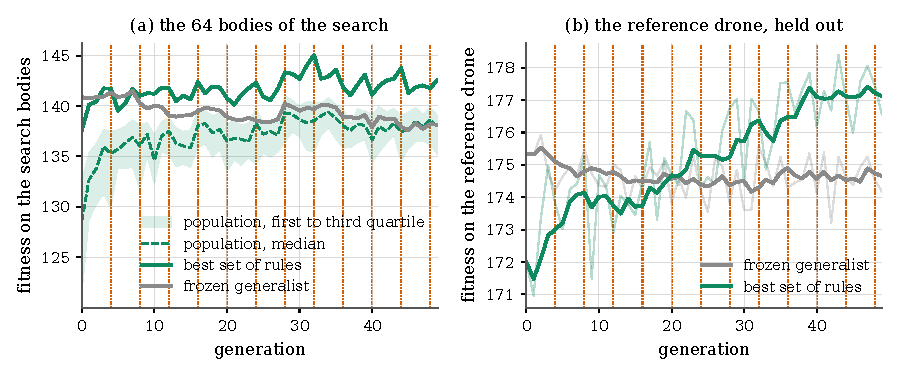
\includegraphics[width=\textwidth]{images/06_Results_and_Experiments/inner_loop/inner_loop_bodies.pdf}
\caption[The inner loop on 64 random bodies]{The inner loop on 64 random bodies. (a) Fitness on the bodies of the search: the best of the 64 sets of rules of each generation, the population's median with a band from the first to the third quartile, and the frozen generalist on the same bodies and forests. The dotted lines mark the refreshes of the bodies. (b) The best set of rules of each generation and the frozen generalist on the reference drone, which the search never flies, over 4\,096 new forests per generation; thin lines are the raw values, thick lines a moving average over five generations.}
\label{fig:inner-loop-bodies}
\end{figure}

\autoref{fig:inner-loop-bodies}(a) shows the fitness on the bodies of the search. At the first generation every one of the 64 sets of rules flies worse than the frozen generalist: the population's median is 129 against 141 for the frozen controller, and its best is 138. This is the starting point that \autoref{subsec:inner-loop} chose. The rules begin as small perturbations of a controller that flies, and a perturbation, on average, costs. From there CMA-ES moves. From the seventh generation on, the best set of rules of each generation is above the frozen controller. Over the last ten generations the best set exceeds the frozen controller by 3.9, 142.2 against 138.2, a gain of about 3\,\%; the step size has shrunk from 0.074 to 0.058 in the meantime. The population's median, however, only catches up with the frozen controller, 137.9 against 138.2 over the same generations, and its upper quartile barely passes it. The search has found a direction in which the rules help, but a random perturbation around that direction still costs about as much as the direction gains. The population as a whole never becomes clearly better than the controller without rules. The curve of the frozen controller is not flat, because at every refresh the bodies change and the new population flies a little differently. This is the reason given in \autoref{subsec:pipeline-run} why the fitness of the rules cannot be compared across updates of the bodies. The comparison that the figure allows is the one that holds at every generation: between the rules and the frozen controller, on the same bodies and forests.

Panel (b) is the same comparison on a body that the search never flies. On the reference drone the best rules of the first generation are worse than the frozen generalist by 3.4, and they remain worse for the first four phases, sixteen generations: rules selected on other bodies do not transfer at once. From the sixth phase on the sign is reversed. Over the last ten generations the best rules exceed the frozen controller by $2.5 \pm 0.6$ on the reference drone, 177.1 against 174.6, or 1.4\,\%. The uncertainty is the spread over generations of the paired difference, each measured on 4\,096 fresh forests. The fitness of the frozen controller alone varies by 0.6 from one generation's forests to the next, so the gain is well above what a draw of forests can produce. The gain is also two thirds of what the rules gain on the bodies they are evolved on. This is the expected direction: part of what a set of rules gains is specific to the bodies on which it was selected.

Decomposed into the quantities of the flights, the held-out gain is of one kind. Progress and the fraction of flights that end in a crash, in the sense of \autoref{subsec:reward}, barely move: 117.2~m against 116.8~m, and 52\,\% of the flights lost against 53\,\%, on a course that ends at five trees per metre. What moves is the speed and the energy. The rules lower the speed by 2\,\%, from 13.9 to 13.6~m/s over commands between 10 and 20~m/s, and they lower the energy per metre more, by 4\,\%. The rules do not make the generalist a better pilot of the reference drone in the sense in which a specialist is one. They make it fly the same course, with the same losses, a little slower and cheaper, and the reward pays for the change. Its energy term rewards the saving directly. Its tracking term is a bell curve that is flat near the commanded speed, so a flight a few per cent slower costs almost nothing per step, while the flight lasts longer over the same distance. The first generations show the opposite, a cost of transport above that of the frozen controller, and the search passes through it. Which term of the reward the rules end up serving is not decided at the start.

How much of what the generalist loses on the reference drone is this? The specialist trained for that drone gives the measure. In a second run the rules were evolved on the reference drone alone, with the same population and 200 forests for each set of rules, 12\,800 flights per generation, for 200 generations. At every generation the best set of rules, the frozen generalist and the frozen specialist flew 2\,048 fresh forests of the search course. \autoref{fig:inner-loop-reference-generalist} shows the three curves. The frozen generalist scores 174.5 on the reference drone and the specialist 182.2. The gap of 7.7, or 4\,\%, is the price of the compromise of \autoref{sec:challenge-morphology} on a body of ordinary proportions. The rules, evolved on this body alone, recover $3.4 \pm 1.2$ of the gap over the last fifty generations, that is 44\,\% of it. The gain appears within the first twenty generations, reaches 3 by the sixtieth and hardly moves afterwards. The gap itself depends on which specialist is used as the measure. The three specialists that were trained score 182.2, 189.7 and 182.4 on the same kind of forests (\autoref{subsec:results-specialist}), so the rules recover between a quarter and a half of what a specialist has over the generalist.
% PROVENANCE: logs/runs_hebbian/2026-09-24_20-15-15_rules_on_generalist_s5535 (local, 200 gens, seed 5535, specialist r1;
% 22:15 → 03:17 on 2026-09-25, exit 0). Window = generations 150 to 199. inner_loop_stats.json, "G"[first entry].

\begin{figure}[htbp]
\centering
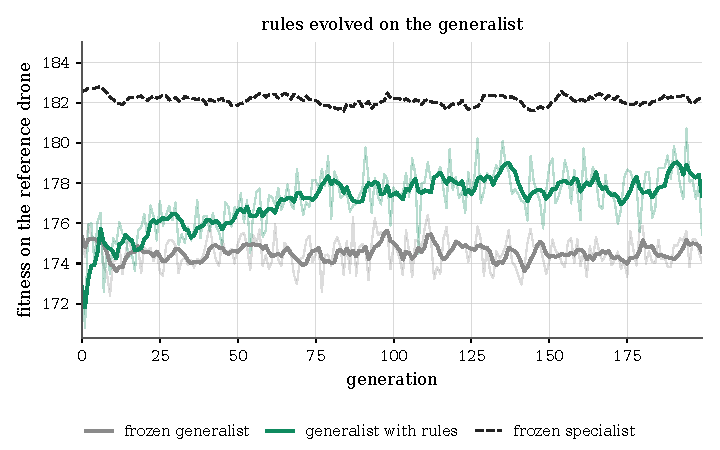
\includegraphics[width=0.8\textwidth]{images/06_Results_and_Experiments/inner_loop/inner_loop_reference_generalist.pdf}
\caption[The inner loop on the reference drone alone, generalist base]{The inner loop on the reference drone alone, with the generalist as base: fitness of the best set of rules of each generation, of the frozen generalist and of the frozen specialist, over 2\,048 new forests per generation flown by all three. Thin lines are the raw values, thick lines a moving average over five generations.}
\label{fig:inner-loop-reference-generalist}
\end{figure}

But the two gains are of a different kind. The specialist loses 28\,\% of its flights where the generalist loses 53\,\%, and it covers 124~m where the generalist covers 117~m. It flies at much the same speed, 14.0 against 13.9~m/s, and it spends more per metre, with a cost of transport of 0.32 against 0.28. The rules leave the losses and the progress where the generalist has them, and they lower the cost of transport by 9\,\%, to 0.26, at a speed 3\,\% lower. Measured in reward, the rules recover over two fifths of the gap. Measured in what the body does, they recover none of the specialist's advantage, which lies in avoiding the trees, and they find instead an economy that the specialist never looked for. In the terms of the objectives of \autoref{subsec:outer-loop} the two changes are not on the same axis. The specialist moves the body along progress and pays for it in energy; the rules move it along the cost of transport at constant progress. This is the approximate correspondence between the reward and the objectives of which \autoref{subsec:reward} warned, seen from the side of the search: a change that the reward pays for need not be the change that a specialist would have made.

Two further observations from this run are used later. The first concerns the selection. The fitness with which the best set of rules is selected, on the forests of the search, is 182.0 over the last fifty generations, against 177.9 for the same set of rules on the held-out forests. The maximum of 64 noisy measurements is thus optimistic by about 4, and a set of rules that is the best of its generation by that margin has often only been lucky on that generation's forests. This is one of the reasons why the pipeline evaluates the bodies on new forests and under eight sets of rules rather than one (\autoref{subsec:outer-loop}). The second concerns repeatability. The run was repeated twice with the same seed, for 100 and for 200 generations, and once with another seed for 200. Runs with the same seed diverge in the simulator, as every run does (\autoref{subsec:genesis-proscons}). The three repeats nevertheless agree with the first run in the result, with gains of 3.0, 4.5 and $3.6 \pm 1.0$ over their last quarters and the same decomposition into speed and energy.
% PROVENANCE: winner's curse = search_best_last - val_best_last of the 200-gen run; repeats = run C
% logs/runs_hebbian/2026-07-08_09-59-42_validation_wspecialis_15_no_bix_15_lstm (100 gens, gain gens 75-99 +3.0) and run B
% logs/runs_hebbian/2026-06-10_10-40-16_validation_wspecialist_no_bix_15_lstm (200 gens, gain gens 150-199 +4.5; its
% "specialist" line is a 25-step specialist and is not used) and the second seed logs/runs_hebbian/2026-09-25_09-11-59_rules_on_generalist_s5536
% (200 gens, seed 5536, specialist r0 as third line: gain gens 150-199 +3.57 ± 0.97, CoT 0.261/0.285, speed 13.33/13.89).

\subsection{Improving Performance on Specialist Controllers}
\label{subsec:results-specialist}

The second experiment repeats the last one with a specialist in the place of the generalist, once for each of the three specialists trained for the reference drone. The rules are evolved on top of the frozen specialist, on the reference drone, with the same population, the same 12\,800 flights per generation and 200 generations. At every generation the best set of rules, the frozen specialist and the frozen generalist fly 2\,048 fresh forests. Whether the rules can help a specialist was left open in \autoref{subsec:specialist-training}. A specialist was trained for the body it flies. The argument of \autoref{subsec:hebbian-why-output}, that plasticity is selected when something varies between lifetimes, gives the rules nothing to work on here, because the body is the one the weights were trained for. The question is whether a controller that already fits its body leaves the rules anything to improve, and, if it does, what.
% PROVENANCE: logs/runs_hebbian/2026-09-24_16-47-43_rules_on_specialist_r1_s5535 (first specialist), 2026-09-25_01-17-04_rules_on_specialist_r0_s5536
% (second), 2026-09-25_05-45-56_rules_on_specialist_r2_s5537 (third); local, seeds 5535/5536/5537, all exit 0; the "specialist_*" columns of their
% validation_summary.csv hold the frozen generalist. Window = generations 150 to 199. inner_loop_stats.json, "S". Generalist row of the table = run 2.

\begin{table}[htbp]
\centering
\small
\begin{tabularx}{\textwidth}{>{\raggedright\arraybackslash}X r r r r r r r r r}
\hline
 & \multicolumn{4}{c}{frozen} & \multicolumn{5}{c}{with the best rules} \\
Base controller & fitness & speed & CoT & crashes & fitness & gain & speed & CoT & crashes \\
\hline
generalist & 174.5 & 13.9 & 0.285 & 53\,\% & 177.9 & +3.4 & 13.4 & 0.259 & 53\,\% \\
first specialist & 182.2 & 13.9 & 0.320 & 28\,\% & 191.9 & +9.6 & 13.3 & 0.257 & 28\,\% \\
second specialist & 189.7 & 13.3 & 0.215 & 31\,\% & 190.2 & +0.5 & 13.3 & 0.212 & 34\,\% \\
third specialist & 182.4 & 13.9 & 0.344 & 29\,\% & 192.3 & +9.9 & 13.3 & 0.243 & 28\,\% \\
\hline
\end{tabularx}
\caption[The four base controllers on the reference drone, frozen and with the best rules]{The four base controllers on the reference drone, frozen and with the best set of rules of each generation, over the last fifty generations of their runs: fitness, mean speed along the corridor in m/s, cost of transport and fraction of flights ended by a crash, on 2\,048 new forests per generation. The gain is the difference in fitness between the two, measured on the same forests; its spread over generations is 1.2, 1.2, 1.0 and 0.8 from top to bottom.}
\label{tab:inner-loop-bases}
\end{table}

\begin{figure}[htbp]
\centering
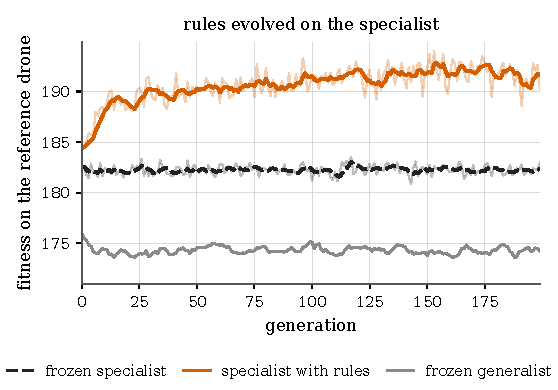
\includegraphics[width=0.62\textwidth]{images/06_Results_and_Experiments/inner_loop/inner_loop_reference_specialist.pdf}
\caption[The inner loop on the reference drone alone, specialist base]{The inner loop on the reference drone alone, with the first specialist as base: fitness of the best set of rules of each generation, of that specialist frozen and of the frozen generalist, over 2\,048 new forests per generation flown by all three. Thin lines are the raw values, thick lines a moving average over five generations.}
\label{fig:inner-loop-reference-specialist}
\end{figure}

\autoref{tab:inner-loop-bases} gives the answer, and it is not the same for the three specialists. On the first and the third specialist the rules add more than anywhere else in this section: $9.6 \pm 1.2$ and $9.9 \pm 0.8$, over 5\,\%, three times what they added to the generalist. \autoref{fig:inner-loop-reference-specialist} shows the first specialist. The rules are above the frozen specialist from the first generation, by 1.8 at generation 0 and by 4.3 over the first ten generations. The gain reaches 7.8 by the fortieth generation and 9.0 by the hundredth, and the third specialist follows the same course. On the second specialist the rules add nothing: $0.5 \pm 1.0$, negative over the first ten generations and inside the noise ever after.

The frozen controllers explain the difference. The three specialists were trained with the same settings and differ in the random seed alone, and they did not arrive at the same way of flying the reference drone. The first and the third fly it at 13.9~m/s with a cost of transport of 0.32 and 0.34, dearer than the generalist. The second flies it at 13.3~m/s with a cost of transport of 0.215, and it scores 7.5 more than the other two for it, with the same progress and the same crashes. The rules bring the first and the third specialist down to 13.3~m/s and to a cost of transport of 0.26 and 0.24, with progress and crashes untouched, as they brought the generalist from 13.9 to 13.4~m/s and from 0.285 to 0.259. The second specialist is there already, and the rules leave it where it is. Two further differences from the generalist's run are worth noting on the first specialist. The gain is there from the start, in the first generation, which is drawn with the same seed in the two runs; on the generalist, the best of the first generation was worse than the controller without rules. And the selection is less deceived by its own forests: the best fitness on the search forests exceeds the held-out fitness of the same rules by 2.5 instead of 4. The flights of a specialist vary less from one forest to the next, as its fewer crashes suggest.

Where the four bases end up is the remarkable part, and \autoref{tab:inner-loop-bases} shows it. Under their respective rules, the generalist and the three specialists all fly the reference drone at the same speed, 13.3 to 13.4~m/s, three of them down from 13.9~m/s. The cost of transport ends between 0.21 and 0.26, in the order in which the frozen controllers had it, and progress and crashes stay where each frozen controller had them. The rules do not move each controller by a fixed amount. They move each controller towards a slower and cheaper flight of the same course, the flight that the fitness of \autoref{subsec:inner-loop} rewards on this body. What each controller gains is the distance it had to travel to get there: nothing for the specialist that was there already, 3.4 for the generalist, about ten for the two specialists that flew fastest and dearest. Why the training reached this point with one seed and not with the other two, the experiment does not say. The training optimizes the discounted return of \eqref{eq:generalist-objective} from randomized releases, and the search optimizes the reward summed over a flight from a fixed release; the two are not the same measure of a flight.

This is how the gains of this section are to be read. \emph{Where a base controller ends up under the rules does not depend on where it started.} The speed at which the rules settle, and the slower and cheaper flight that goes with it, are a property of the body and of the fitness rather than of the controller, and a controller gains what it had to travel to get there. On a fixed body, then, the rules do what \autoref{sec:hebbian-controller} asked of them. They take a controller trained for all bodies, or a controller trained for this body but to a different flight, and they fit it to the flight of this body that the fitness rewards. They do so within a few tens of generations, on any base that is not there already. The gain is real in the currency of the outer loop, because a lower cost of transport at equal progress is a better point in objective space. What a fixed body cannot show is the case that \autoref{subsec:hebbian-why-output} made for plasticity: a body that differs from one flight to the next, which the controller must fit without being told which one it is. That is what \autoref{sec:codesign-experiments} is for.

\section{Full Co-Design Experiments}
\label{sec:codesign-experiments}

The second part of the chapter runs the pipeline of \autoref{sec:pipeline} as a whole and compares it with the control of \autoref{subsec:pipeline-control}. Eight co-design runs and eight morphology-only runs were made with the settings of \autoref{tab:pipeline-settings}, on six random seeds. For each seed a run of both conditions exists, and the two start from the same 64 random bodies. Two seeds carry a second co-design run in which a phase lasts six generations instead of four, so that the run holds 33 phases instead of 50. These two runs enter every comparison that treats the runs as independent, and they are left out of the paired analysis of \autoref{subsec:results-pca}. The morphology-only runs, whose bodies are updated at every generation, have 88 generations, 87 exams and 5\,568 examined bodies, against 49 exams and 3\,136 bodies for a co-design run. They took about 130 hours of the node against 94.
% PROVENANCE: co-design = logs/remote/outer_nsga/outer_exam_4_64_64_300_{r0,r1} (seeds 67, 68), outer_exam_6_64_64_300_{r0,r1}
% (seeds 67, 68, refresh 6), outer_exam_4_64_64_300_extra_r{0..3} (seeds 12345..12348); morphology-only = outer_morphology_only_exam_r{0..3}
% (seeds 67..70), outer_morphology_only_exam_extra_r{0..3} (12345..12348). Wall-clock: THESIS_DECISIONS.md section 6.

What a run leaves behind is the archive of \autoref{subsec:pipeline-run}: every body it examined, with the two objectives measured on the exam course under the sets of rules of the moment. The result of a run is read from this archive as its \emph{cumulative front}: the set of examined bodies that passed the 80~m gate and are dominated by no other examined body of the same run. The cumulative front is the best trade-off between progress and cost of transport that the run found, at whatever phase it found it. The point of comparison in every figure is the reference drone flown by the frozen generalist on the same course, measured at every exam as described in \autoref{subsec:outer-loop}: 190.8~m at a cost of transport of 0.288, the same in every run.

Fronts are sets, and comparing two groups of eight fronts needs indicators. Two are used, both read off a front at a fixed value of the other objective: the cost of transport of the cheapest body that reaches a given progress, and the progress of the farthest body within a given cost of transport. They are the attainment functions of Fonseca and Fleming \cite{fonseca1996performance, lopezibanez2010exploratory} read at one level. They answer the practical questions directly: what it costs to fly 170~m through this forest with the best body each search found, and how far a body within a given budget goes. The hypervolume of \autoref{subsec:nsga2} is used as well, with the reference point at 80~m of progress, the gate, and at a cost of transport of 0.5, above every body of every front. The unit of every test is the run. With eight runs in each group, the rank-sum test of Mann and Whitney \cite{mann1947test} is used in its exact form, in which the p-value is computed over all 12\,870 ways of assigning the sixteen runs to two groups of eight. The smallest p-value the test can return is 0.00016, reached when every run of one group is better than every run of the other; it is written as p-value $< 0.001$. The size of a difference is given as the Hodges--Lehmann shift \cite{hodges1963estimates}: the median of the 64 differences between a run of one group and a run of the other. The shift is reported with its exact 95\,\% confidence interval. Where an indicator is read at every progress level along the front, the p-values are adjusted for the family of levels by the resampling procedure of Westfall and Young \cite{westfall1993resampling}.
% PROVENANCE: WP2_Outer_Loop.pareto_stats (logs/remote/outer_nsga/pareto_stats/, README.md + summary.json), pareto_overlay/.

\subsection{Co-Design vs. Morphology-Only Evolution}
\label{subsec:results-codesign-vs-morph}

\begin{figure}[htbp]
\centering
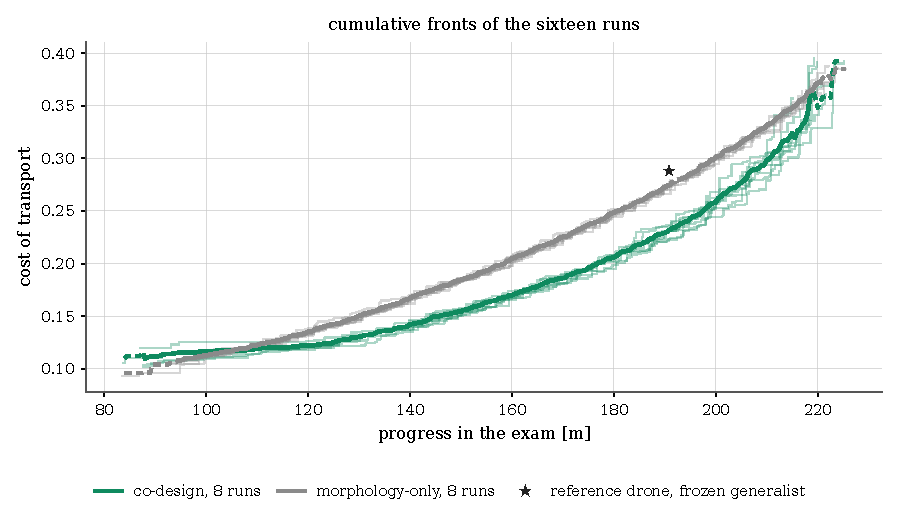
\includegraphics[width=\textwidth]{images/06_Results_and_Experiments/codesign/codesign_fronts.pdf}
\caption[The cumulative fronts of the sixteen runs]{The cumulative fronts of the sixteen runs on the exam course, co-design in green and morphology-only in grey. Thin lines are the fronts of the single runs; the thick line of each condition is, at every progress, the mean over its runs of the cost of transport of the cheapest body that reaches that progress, drawn solid where at least four of the eight fronts reach it and dashed where fewer do. The star is the reference drone flown by the frozen generalist.}
\label{fig:codesign-fronts}
\end{figure}

\autoref{fig:codesign-fronts} shows the sixteen cumulative fronts and, for each condition, the mean cost of transport at every progress over the runs whose front reaches it. The two families agree at their ends. At the tip, the farthest body of a run averages 213 to 225~m over its exam flights in the co-design runs and 217 to 226~m in the control (p-value 0.44). No body of either condition gets, on average, past 226~m of the 300~m course, so the tip is set by the forest rather than by the search. At the cheap end, the arm of bodies that fly 85 to 110~m for a cost of transport of 0.10 to 0.12 is the same in both conditions, and three co-design runs have no body below 128~m. Between the two ends the fronts separate, and the separation is the result of this section. From 128 to 213~m of progress the co-design fronts are cheaper at every level, with an adjusted p-value below 0.05 along the whole band. At 130, 150, 170, 190 and 210~m every one of the eight co-design runs is cheaper than every one of the eight control runs (\autoref{fig:codesign-indicators}(a), \autoref{tab:codesign-indicators}). The gap is about a sixth of the cost. At 150, 170 and 190~m the shift is $-0.031$, $-0.039$ and $-0.044$, that is 17, 17 and 16\,\% of what the control's bodies spend at those distances. The gap narrows to 12\,\% at 130~m, where the fronts begin to merge into the common arm, and to 10\,\% at 210~m, near the common tip. Read the other way, in \autoref{fig:codesign-indicators}(b), a body within a cost of transport of 0.15, 0.20 or 0.25 flies 16, 18 and 16~m farther on a co-design front than on a control front, 12, 11 and 9\,\% more. At 0.30 the gain is 10~m. At 0.35, where both fronts have reached their tips, it is 1.5~m and not significant.
% PROVENANCE: pareto_stats/summary.json (indicators, attainment band 128-213 m, progress band CoT 0.1475-0.335), indicators_per_run.csv.

\begin{figure}[htbp]
\centering
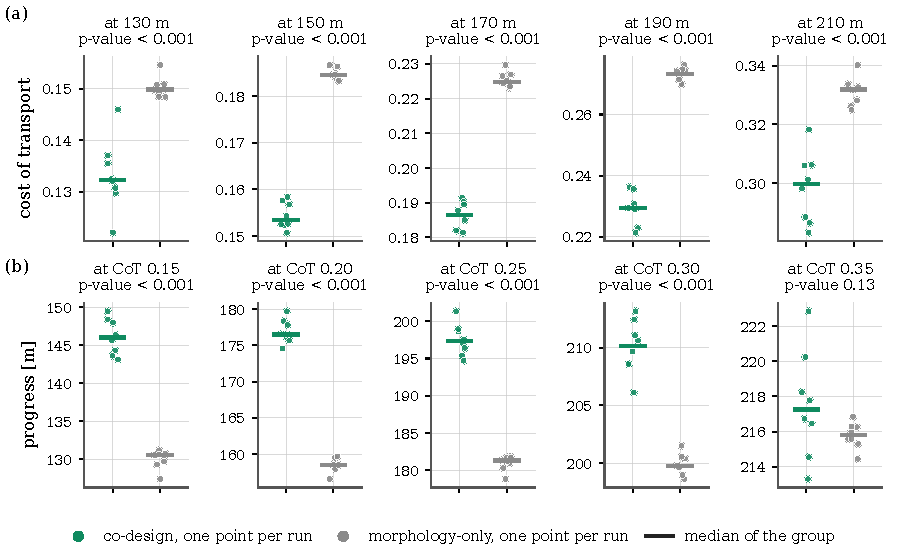
\includegraphics[width=\textwidth]{images/06_Results_and_Experiments/codesign/codesign_indicators.pdf}
\caption[The fronts read at fixed progress and at fixed cost of transport]{The fronts read at fixed progress and at fixed cost of transport, one point per run and the median of each group as a bar. (a) Cost of transport of the cheapest body of the front that reaches 130, 150, 170, 190 and 210~m. (b) Progress of the farthest body of the front within a cost of transport of 0.15, 0.20, 0.25, 0.30 and 0.35. The p-values are those of the exact rank-sum test over the sixteen runs.}
\label{fig:codesign-indicators}
\end{figure}

\begin{table}[htbp]
\centering
\small
\begin{tabularx}{\textwidth}{>{\raggedright\arraybackslash}X r r r r r}
\hline
Indicator & Co-design & Morphology-only & Shift & 95\,\% CI & p-value \\
\hline
CoT at 150~m & 0.153 & 0.185 & $-0.031$ & $-0.033$ to $-0.027$ & $< 0.001$ \\
CoT at 170~m & 0.186 & 0.225 & $-0.039$ & $-0.043$ to $-0.035$ & $< 0.001$ \\
CoT at 190~m & 0.229 & 0.273 & $-0.044$ & $-0.049$ to $-0.039$ & $< 0.001$ \\
Progress at CoT 0.15 & 146.0 & 130.5 & $+15.9$ & $+13.7$ to $+18.3$ & $< 0.001$ \\
Progress at CoT 0.20 & 176.5 & 158.5 & $+18.1$ & $+17.0$ to $+19.9$ & $< 0.001$ \\
Progress at CoT 0.25 & 197.3 & 181.3 & $+16.2$ & $+14.5$ to $+18.2$ & $< 0.001$ \\
Progress of the tip & 219.5 & 220.6 & $-1.4$ & $-5.4$ to $+2.9$ & 0.44 \\
Hypervolume & 44.8 & 41.9 & $+2.7$ & $+2.0$ to $+3.3$ & $< 0.001$ \\
\hline
\end{tabularx}
\caption[Indicators of the cumulative fronts, eight runs against eight]{Indicators of the cumulative fronts, eight runs against eight: the median over the runs of each condition, the Hodges--Lehmann shift of co-design against morphology-only with its exact 95\,\% confidence interval, and the p-value of the exact rank-sum test; the single runs are shown in \autoref{fig:codesign-indicators} and \autoref{fig:codesign-hv}. CoT is the cost of transport of the cheapest body of the front that reaches the given progress; progress, in metres, is that of the farthest body within the given cost of transport; the hypervolume is measured from the reference point at 80~m and a cost of transport of 0.5.}
\label{tab:codesign-indicators}
\end{table}

Against the reference drone, both searches find bodies that fly farther for less, but not by the same margin. The reference drone, a body of ordinary proportions flown by the generalist, lies on the mean front of the search under that generalist. The control improves on it along the front, in range and in economy at short distances, but hardly at the reference drone's own operating point. There, the cheapest body of a control run costs 0.270 to 0.276 against the reference drone's 0.288, that is 3 to 6\,\% less. The cheapest co-design body at the same 191~m costs 0.221 to 0.236, 16 to 22\,\% less.
% PROVENANCE: batch_5 brief (memory project_batch5_replication): star 190.8 m / 0.288 in all 16 runs; CoT@190 per run in indicators_per_run.csv.

\begin{figure}[htbp]
\centering
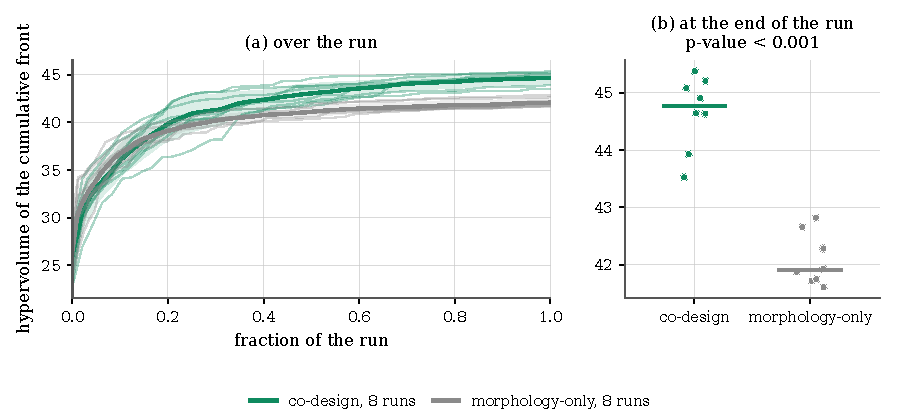
\includegraphics[width=\textwidth]{images/06_Results_and_Experiments/codesign/codesign_hv.pdf}
\caption[Hypervolume of the cumulative fronts]{Hypervolume of the cumulative fronts, reference point at 80~m and a cost of transport of 0.5. (a) Over the course of the runs, on the axis of the fraction of the run that is completed, since a co-design run holds 50 or 33 exams and a control run 87: thin lines are the single runs, thick lines the mean of each condition with a band of one standard deviation. (b) At the end of the runs, one point per run.}
\label{fig:codesign-hv}
\end{figure}

The hypervolume tells the same story in one number and adds its time course (\autoref{fig:codesign-hv}). At the end of the runs it is 43.5 to 45.4 in the co-design runs and 41.6 to 42.8 in the control, with medians of 44.8 and 41.9. The shift is $+2.7$, with a confidence interval of $[2.0, 3.3]$ and no overlap between the groups. Over the run the two curves start from the same value, since the first population is the same. The control leads for the first sixth of the run, because its bodies are updated at every generation and its first exams come faster. The co-design curve overtakes it at about a fifth of the run. The difference between the group means is significant from 36\,\% of the run to the end, after adjustment for the number of points at which it is read. The control was given more of everything that concerns the bodies, 87 exams against 49 and 5\,568 examined bodies against 3\,136, and it does not catch up.
% PROVENANCE: pareto_stats/hv_time_test.csv (cumulative HV significant from 36 % of the run), summary.json "hypervolume", exam_hv_runs_fraction_aggregate.csv.

In the terms of \autoref{ch:challenges} the comparison is as clean as the pipeline allows. The two conditions start from the same bodies, use the same operators, the same exam course and the same gate, and the control is given the larger budget. The only difference is that in one condition the 896 coefficients are searched and in the other they are held at zero. The fronts differ where there was room for them to differ, between the arm that the gate cuts and the tip that the forest sets. They differ by up to 17\,\% of the energy per metre at equal progress and by up to 12\,\% of the progress at equal energy. \emph{This answers the question with which \autoref{sec:challenge-feasibility} closed: an adaptation that costs no more than the flights that score a body is enough to change the outcome of the search.} What it does not say is whether the outcome is a different set of bodies, or the same bodies flown better by the rules they were selected with. The next three subsections take the question apart.

\subsection{Swapping the Pareto Fronts}
\label{subsec:results-swapped-fronts}

A front of the co-design pipeline is a front of pairs: bodies selected under the rules of the moment, and rules selected on those bodies. To separate the two, the bodies of a front are flown again under a controller they were not selected with. The last front of four co-design runs and of four morphology-only runs, 37 to 44 bodies each, was rebuilt from the genomes and flown on the exam course over 256 new forests. Two controllers flew every body on the same forests: the frozen generalist, and the Hebbian controller with the best set of rules of a co-design run. On a co-design front these are the run's own rules, the ones its bodies were selected with. The control runs have no rules of their own, so the bodies of their fronts were flown with the best set of rules of one of the co-design runs, the second of the four, transplanted as they were. Of the four sets of rules, that one helps the reference drone most when transplanted to it: by 9~m, against 1 to 2~m for the other three. The choice therefore does not favour the conclusion that follows. \autoref{fig:swapped-fronts} shows one front of each kind and \autoref{tab:swapped-fronts} the eight.
% PROVENANCE: <run>/comparisons_hebbian/README.md of outer_exam_4_64_64_300_r{0,1}, outer_exam_6_64_64_300_r{0,1}, outer_morphology_only_exam_r{0..3}
% (WP2_Outer_Loop.transfer_eval, 2026-08-21, 256 forests with --forest-seed 0, exam course; the transplanted rules are exam_4_r1's best genome).
% Standard drone under the four runs' rules: 180.1 / 188.0 / 179.9 / 180.9 m against 179.3 m frozen (standard_hebbian.csv).

\begin{figure}[htbp]
\centering
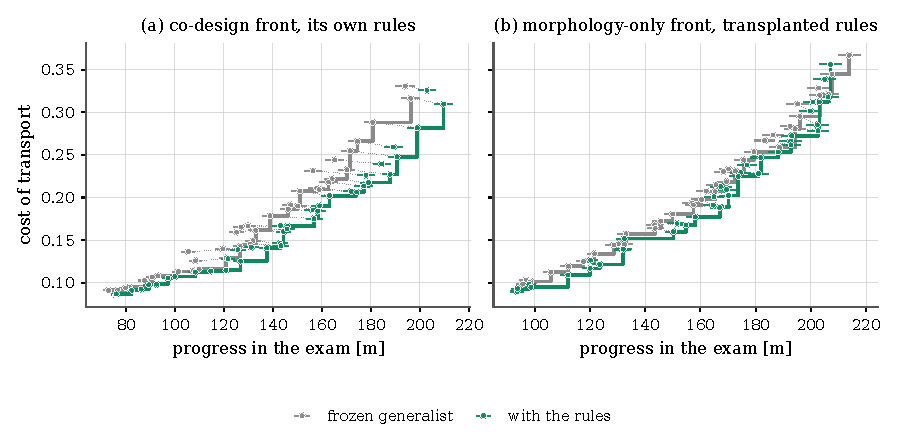
\includegraphics[width=\textwidth]{images/06_Results_and_Experiments/codesign/swapped_fronts.pdf}
\caption[Front bodies flown by the frozen generalist and by the Hebbian controller]{The bodies of a last front flown again on the exam course, over the same 256 forests, by the frozen generalist (grey) and by the Hebbian controller with the best set of rules of a co-design run (green); each body is one point in both colours, joined by a dotted line, with the standard error of its progress as a bar, and the steps are the fronts of the two sets of points. (a) A co-design front under its own rules. (b) A morphology-only front under the same rules, transplanted.}
\label{fig:swapped-fronts}
\end{figure}

\begin{table}[htbp]
\centering
\small
\begin{tabularx}{\textwidth}{>{\raggedright\arraybackslash}X r r r r r}
\hline
Front & Bodies & Rules & Progress [m] & Bodies farther & CoT \\
\hline
co-design, first run & 37 & its own & $+19.3 \pm 1.7$ & 33 & $+0.001 \pm 0.001$ \\
co-design, second run & 39 & its own & $+11.7 \pm 0.9$ & 38 & $-0.003 \pm 0.000$ \\
co-design, third run & 42 & its own & $+11.8 \pm 0.8$ & 41 & $-0.008 \pm 0.001$ \\
co-design, fourth run & 43 & its own & $+8.8 \pm 0.7$ & 43 & $-0.004 \pm 0.000$ \\
morphology-only, first run & 40 & transplanted & $+3.2 \pm 0.7$ & 28 & $-0.006 \pm 0.000$ \\
morphology-only, second run & 44 & transplanted & $+6.3 \pm 0.7$ & 38 & $-0.005 \pm 0.000$ \\
morphology-only, third run & 44 & transplanted & $+1.1 \pm 1.1$ & 25 & $-0.006 \pm 0.000$ \\
morphology-only, fourth run & 43 & transplanted & $+3.1 \pm 0.8$ & 30 & $-0.006 \pm 0.000$ \\
\hline
\end{tabularx}
\caption[What the rules add to the bodies of a front]{What the rules add to the bodies of a front: change of the mean progress and of the cost of transport of the front's bodies when they are flown by the Hebbian controller instead of the frozen generalist, on the same 256 forests of the exam course, with the standard error of the mean over the bodies, and the number of bodies that fly farther under the rules. The co-design fronts are flown with the rules of their own run, the morphology-only fronts with the rules of the second co-design run.}
\label{tab:swapped-fronts}
\end{table}

On the bodies they were selected with, the rules add 9 to 19~m of progress, and all but a handful of the bodies of every front fly farther. The front of a co-design run under its own rules lies to the right of the same bodies under the frozen generalist along its whole length (\autoref{fig:swapped-fronts}(a)). On the bodies of a morphology-only front the same rules add 1 to 6~m, three to four times less, and on one front they add nothing that the 256 forests can resolve; the two fronts of panel (b) nearly coincide in progress. What transfers is the economy. The cost of transport falls by 0.005 to 0.006 on every front of the control, on almost every body, as it falls on two of the four co-design fronts. This is the saving that \autoref{sec:inner-loop-experiments} found the rules give to any base controller on a fixed body. The progress does not transfer. The rules let a co-design front fly farther than the generalist would fly it, but only on the bodies they were evolved with, and not on bodies that were selected under the generalist. \emph{A co-design front is therefore not the front of the generalist with a better controller on top.} The rules have specialized to the family of bodies that the outer loop retained, and the bodies were retained because the rules fly them, so what the front holds is the pair. This is the reversal of \eqref{eq:ranking-flip} seen from its far side: a body selected under an adapting controller is one whose value shows with a controller adapted to it.

\subsection{PCA Analysis of the Evolved Morphologies}
\label{subsec:results-pca}

If the co-design front holds pairs, the bodies of the two conditions can be compared directly, in the space of the genome. Do the two searches, started from the same 64 bodies, go to the same place? The population of a run at each phase is summarized by its centroid in the unit cube of the 15 genes of \autoref{tab:drone-genome}, and a run by the path of that centroid from the first phase to the last. Distances between centroids are taken in the 15 dimensions of the cube. There, a distance of 0.7 corresponds to a difference of about 0.18 on every gene, or 18\,\% of its range. The principal components serve the figure only. For each of the six seeds a PCA is fitted on the centroids of its two runs, and the first two components carry 50 to 58\,\% of their variance (\autoref{fig:pca-seed-pairs}).
% PROVENANCE: WP2_Outer_Loop.pca_trajectories --per-seed (logs/remote/outer_nsga/pca_exam_seed_pairs_independent/, seed_pair_distances.csv,
% seed_pair_pca_variance.csv); joint 14-run distances in pca_exam_seed_paired/final_centroid_distances.csv (refresh-6 runs included there).

\begin{figure}[htbp]
\centering
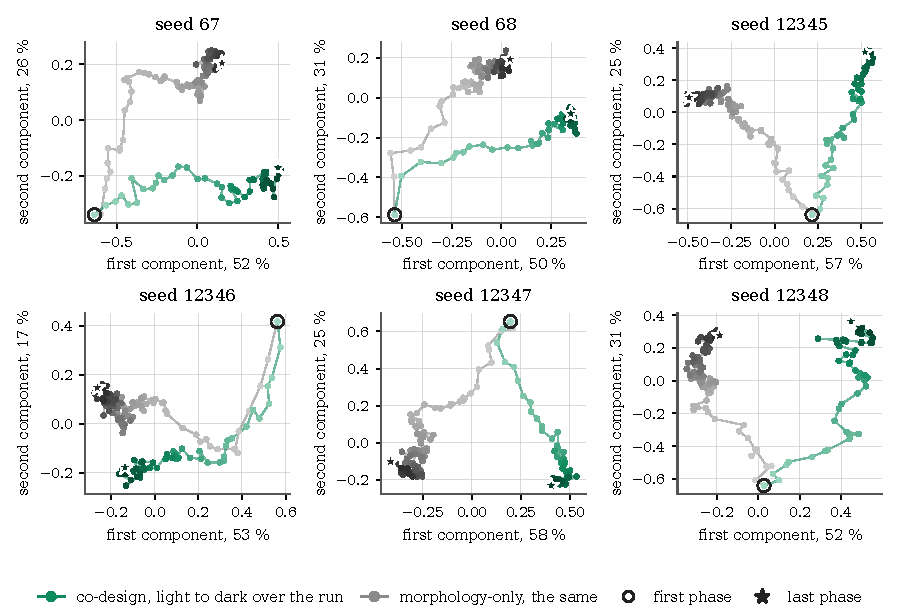
\includegraphics[width=\textwidth]{images/06_Results_and_Experiments/codesign/pca_seed_pairs.pdf}
\caption[The path of the population of the two runs of each seed in the space of the genome]{The path of the population of the two runs of each seed in the space of the genome, one panel per seed: the centroid of the 64 bodies at every phase, from the first (circle) to the last (star), co-design in green and morphology-only in grey, darker as the run proceeds. Each panel has its own principal components, fitted on the centroids of its two runs, with the share of the variance each carries on its axis; the axes are not comparable across panels.}
\label{fig:pca-seed-pairs}
\end{figure}

\begin{table}[htbp]
\centering
\begin{tabularx}{\textwidth}{>{\raggedright\arraybackslash}X r r r}
\hline
Pair of runs & Pairs & Distance & Range \\
\hline
two morphology-only runs & 15 & $0.50 \pm 0.10$ & 0.28 to 0.62 \\
two co-design runs & 28 & $0.70 \pm 0.15$ & 0.38 to 0.99 \\
a co-design and a morphology-only run, same seed & 8 & $0.70 \pm 0.20$ & 0.50 to 1.08 \\
a co-design and a morphology-only run, different seeds & 40 & $0.71 \pm 0.13$ & 0.48 to 1.02 \\
\hline
\end{tabularx}
\caption[Distances between the last populations of the runs]{Distances between the centroids of the last populations of the sixteen runs, in the unit cube of the genome, by kind of pair: mean, standard deviation and range over the pairs. The two co-design runs with phases of six generations are included; the paired distances of the six seeds of \autoref{fig:pca-seed-pairs} are 0.59, 0.50, 1.08, 0.51, 0.90 and 0.69.}
\label{tab:pca-distances}
\end{table}

In every panel of \autoref{fig:pca-seed-pairs} the two runs leave the same point together and part within the first five phases, and in five of the six panels they end in different regions of the space. The sixth pair, on seed 12346, ends 0.51 apart, which is the distance between two morphology-only runs of different seeds (\autoref{tab:pca-distances}). Two things follow from the table. First, the starting bodies do not decide where a run ends. A co-design run is no closer to the control run that started from its own 64 bodies than to a control run that started from others, 0.70 against 0.71. For only one of the eight co-design runs is its seed partner the nearest control run. Second, the two conditions do not scatter alike. The eight morphology-only runs end within 0.28 to 0.62 of each other, in one cluster: under a fixed controller the search over bodies has one optimum, and every run finds it. The co-design runs end 0.38 to 0.99 apart, a spread half as wide again, and three of them end in a region of the space that no control run visits. \emph{The adapting controller does not shift the optimum of the body search by a fixed amount: it changes which bodies come first, as \autoref{sec:challenge-morphology} argued it would, and the bodies it makes reachable are different ones for different runs.} Which bodies these are, in terms a designer can read, is the subject of the next subsection.
% PROVENANCE: memory project_pca_seed_paired_exam_runs (seed partner nearest for 1 of 8: cod6_s68; s12347/s12348/s68 in a high-PC2 region
% no morph-only run visits); distances recomputed 2026-09-29 from final_centroid_distances.csv (co-design 0.696 +- 0.149, morph 0.502 +- 0.095).

\subsection{Morphology Choices of The Evolution}
\label{subsec:results-morphologies}

\begin{figure}[htbp]
\centering
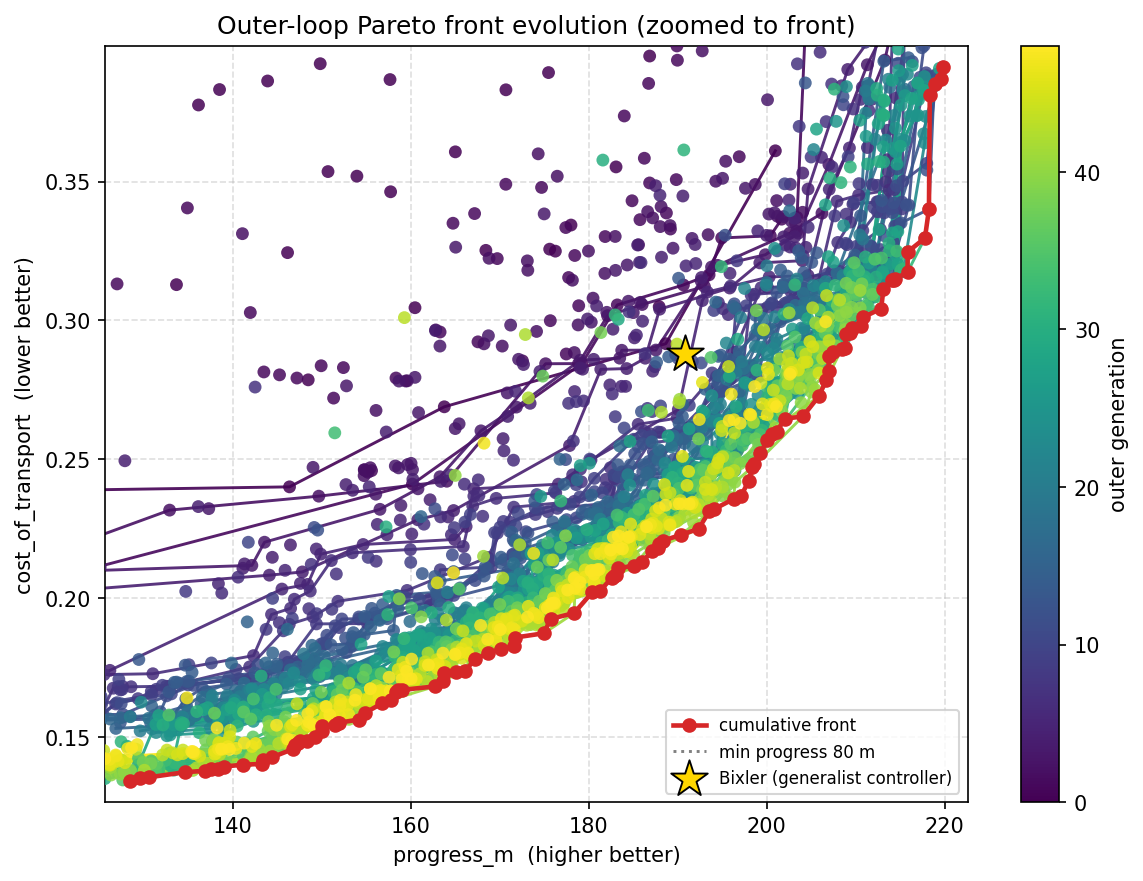
\includegraphics[width=0.8\textwidth]{images/06_Results_and_Experiments/front_evolution/exam4_r0_pareto_front_evolution_zoomed.png}
\caption[The examined bodies of a co-design run]{The examined bodies of the first co-design run in the plane of the objectives, coloured by the phase of their exam, with the cumulative front of the run in red; bodies below 128~m of progress are left out of the view. The lines join the successive exams of the bodies that survived more than one phase.}
\label{fig:front-evolution}
\end{figure}

\autoref{fig:front-evolution} shows what a run does with its bodies: the 3\,136 examined bodies of the first co-design run, coloured by phase. The early exams scatter above the front and the later ones lie along it. The front itself is built over the whole run: its cheap end comes from bodies of the middle phases and its tip from a body of the thirteenth phase. The two ends of a front are two designs, and \autoref{fig:champions} shows the two of this run: the body that flies farthest, 220~m at a cost of transport of 0.39, and the cheapest body that passes the gate, 128~m at 0.13. \autoref{tab:champions} gives their parameters.
% PROVENANCE: outer_exam_4_64_64_300_r0/2026-08-10_21-53-50_.../plots/champion_renders/champions.csv (progress champion phase 13, CoT champion
% phase 35, gated at 80 m), URDF masses parsed from the champion URDFs (0.575 and 1.963 kg, wing links 0.152 and 1.453 kg).

\begin{figure}[htbp]
\centering
\begin{subfigure}[c]{0.48\textwidth}
\centering
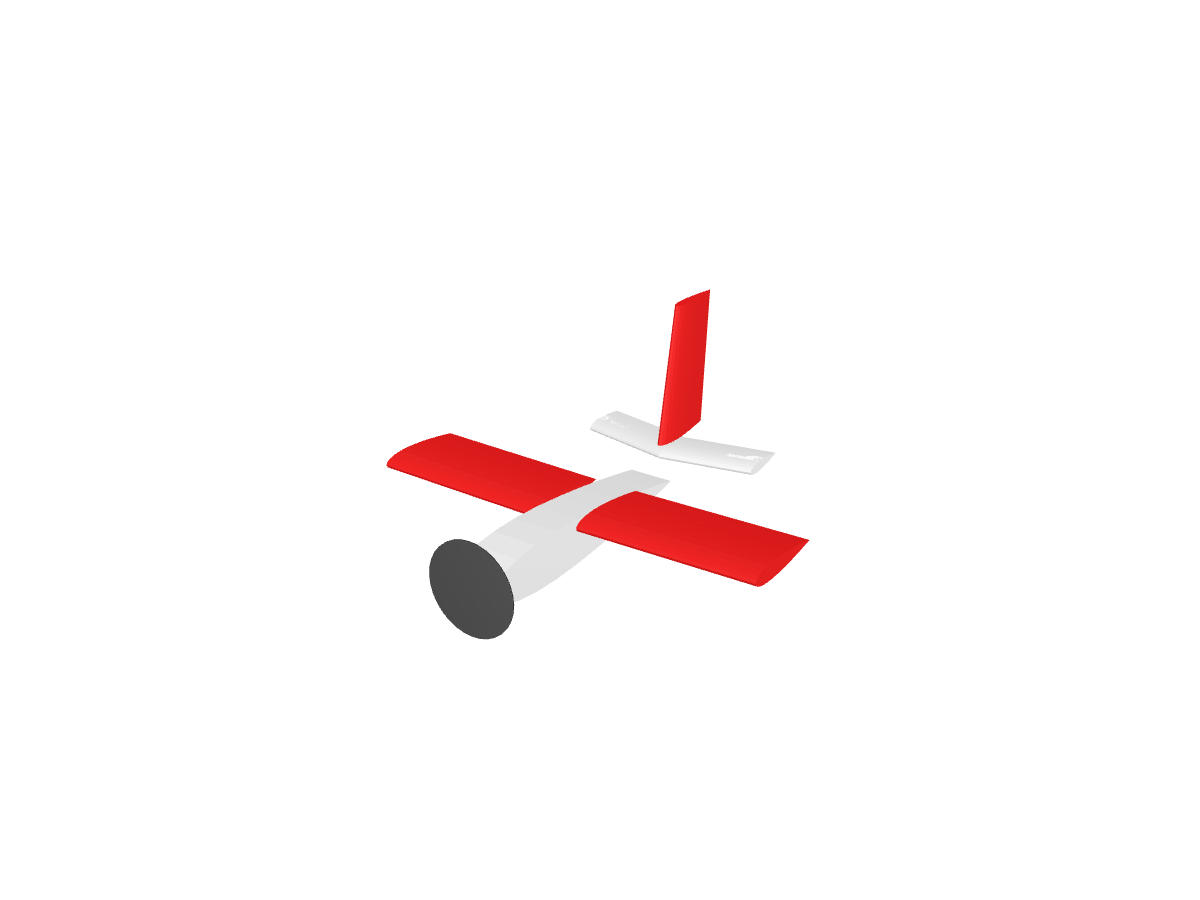
\includegraphics[width=\textwidth, trim={60 100 60 100}, clip]{images/06_Results_and_Experiments/champion_renders/outer_exam_4_64_64_300_r0/progress_champion_gen13_ind_001_3quarter.png}
\caption{}
\label{fig:champions-progress-3q}
\end{subfigure}
\hfill
\begin{subfigure}[c]{0.48\textwidth}
\centering
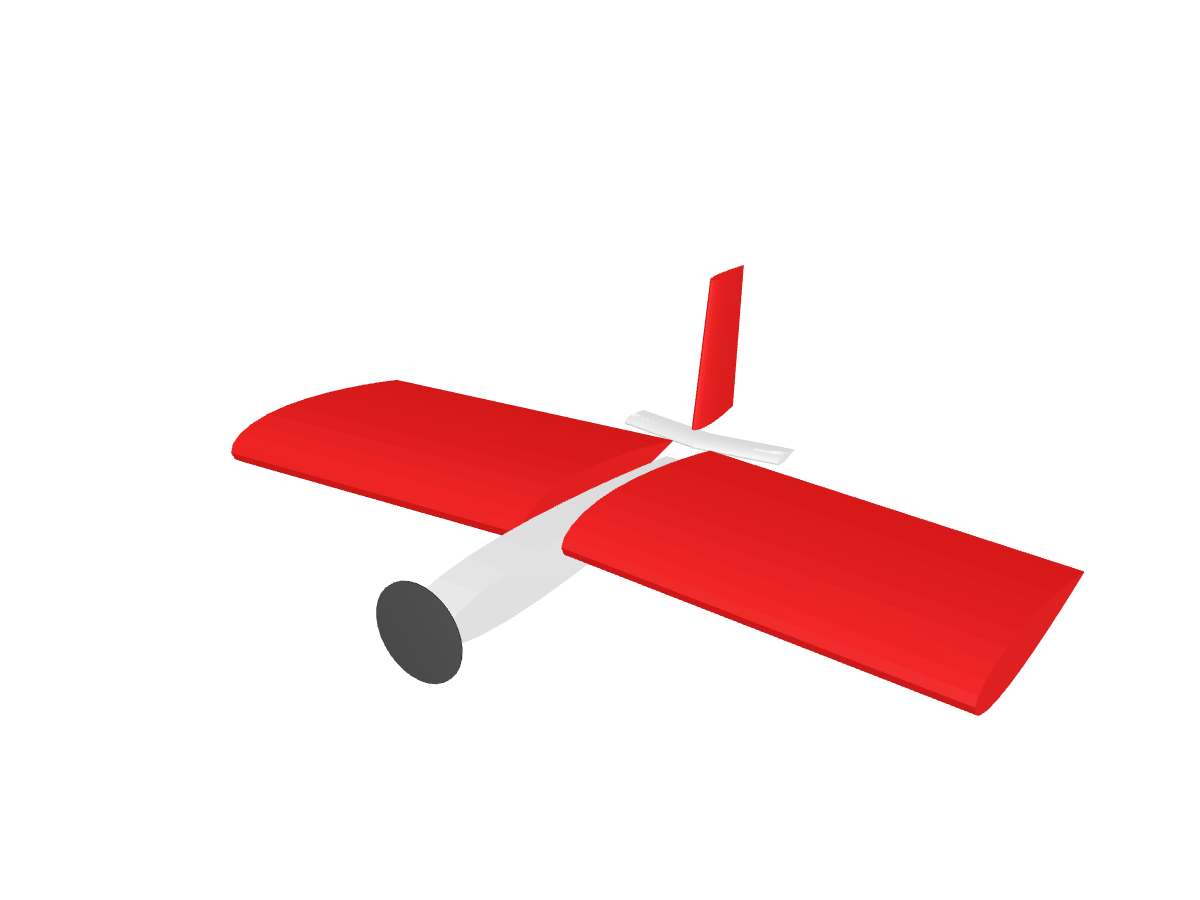
\includegraphics[width=\textwidth, trim={60 100 60 100}, clip]{images/06_Results_and_Experiments/champion_renders/outer_exam_4_64_64_300_r0/cot_champion_gated80m_gen35_ind_000_3quarter.png}
\caption{}
\label{fig:champions-cot-3q}
\end{subfigure}
\begin{subfigure}[c]{0.48\textwidth}
\centering
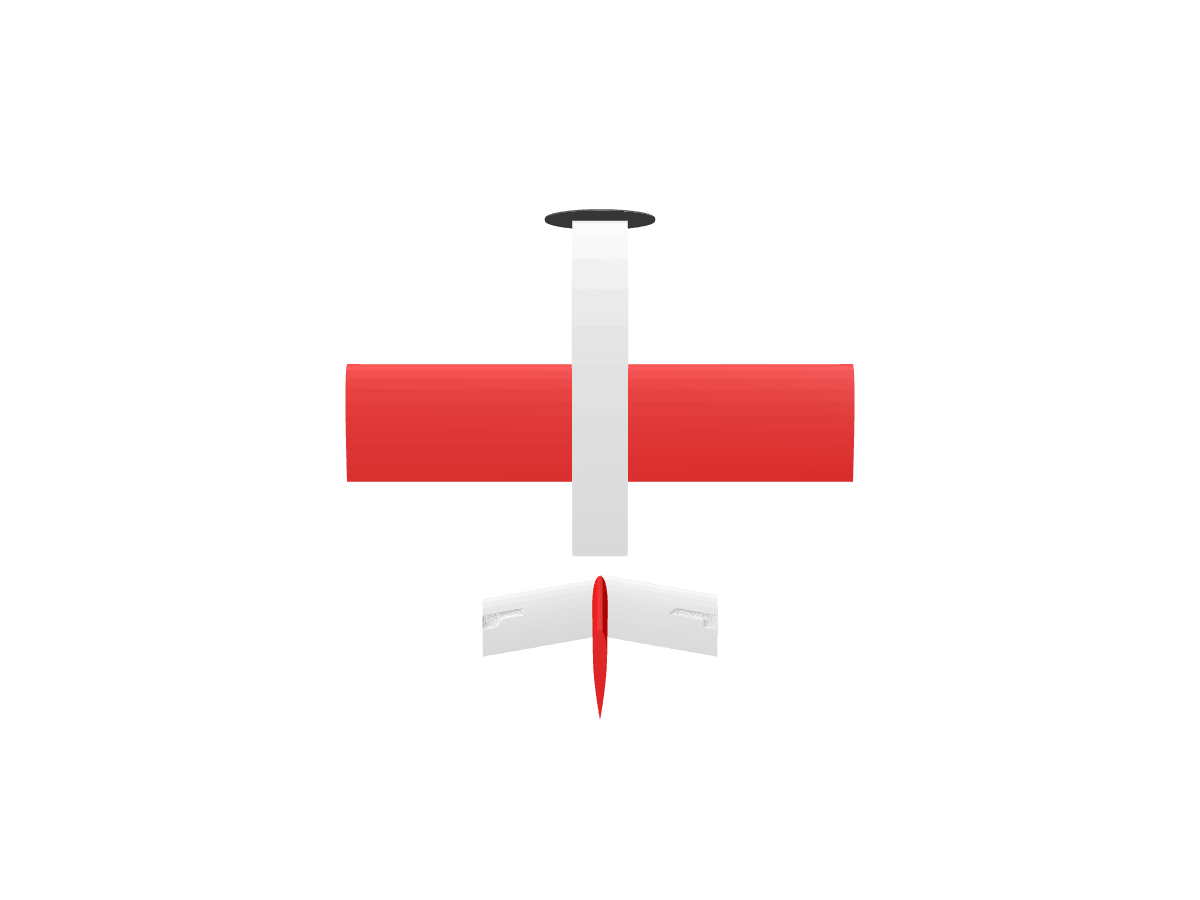
\includegraphics[width=\textwidth, trim={60 100 60 100}, clip]{images/06_Results_and_Experiments/champion_renders/outer_exam_4_64_64_300_r0/progress_champion_gen13_ind_001_top.png}
\caption{}
\label{fig:champions-progress-top}
\end{subfigure}
\hfill
\begin{subfigure}[c]{0.48\textwidth}
\centering

\includegraphics[width=\textwidth, trim={60 100 60 100}, clip]{images/06_Results_and_Experiments/champion_renders/outer_exam_4_64_64_300_r0/cot_champion_gated80m_gen35_ind_000_top.png}
\caption{}
\label{fig:champions-cot-top}
\end{subfigure}
\caption[The two ends of the front of a co-design run]{The two ends of the front of the first co-design run, drawn at one common scale. Left, (a) and (c): the body that flies farthest. Right, (b) and (d): the cheapest body that passes the gate. Three-quarter views above, top views with the nose up below; wing panels and rudder in red, fuselage and elevator in grey.}
\label{fig:champions}
\end{figure}

\begin{table}[htbp]
\centering
\begin{tabularx}{\textwidth}{>{\raggedright\arraybackslash}X r r}
\hline
 & Farthest body & Cheapest body \\
\hline
Progress and cost of transport in the exam & 220~m, 0.39 & 128~m, 0.13 \\
Span of one wing panel & 0.40~m & 0.85~m \\
Chord of the wing & 0.21~m & 0.56~m \\
Wing area, both panels & 0.17~m$^2$ & 0.95~m$^2$ \\
Length of the fuselage & 0.61~m & 0.90~m \\
Centre of mass along the fuselage & 56\,\% & 31\,\% \\
Attachment of the wing along the fuselage & 52\,\% & 56\,\% \\
Span of the elevator, of the rudder & 0.42~m, 0.33~m & 0.41~m, 0.37~m \\
Dihedral & $-0.9^{\circ}$ & $+2.8^{\circ}$ \\
Gear ratios of the sweep, of the twist & 3.19, 2.22 & 3.18, 2.21 \\
Airfoil & NACA 4417 & NACA 4520 \\
Mass, of which the wing & 0.58~kg, 0.15 & 1.96~kg, 1.45 \\
\hline
\end{tabularx}
\caption[The two bodies at the ends of the front of a co-design run]{The two bodies of \autoref{fig:champions}: the genes of \autoref{tab:drone-genome} in physical units, the wing area and the mass of the built body. The chord follows from the span and the aspect ratio of the panel.}
\label{tab:champions}
\end{table}

The two bodies are as different as the design space allows on its main axes, and alike on the others. The body that flies farthest is small and light. It has panels of 0.40~m, a wing of 0.17~m$^2$, a fuselage of 0.61~m and a mass of 0.58~kg in all. Its centre of mass is well aft, at 56\,\% of the fuselage, close to the wing. It is a body with little static margin that turns readily, which is what the dense half of the course rewards, and it pays for the agility with a cost of transport three times that of the other body. The cheapest body is a glider. It has panels of 0.85~m with a chord of 0.56~m, 1.8~m from tip to tip, a wing of almost a square metre that weighs 1.45 of the body's 1.96~kg, a long fuselage with the centre of mass forward, at 31\,\%, and a positive dihedral. All of this makes for a stable and slow flight. Its cost of transport is low partly because it is heavy, since the cost of transport divides the energy by the weight. It does not get through the second half of the course, where the forest thickens past what such a wing can be steered through: it stops at 128~m on average, four metres from the point where the front meets the common arm. The two bodies agree on their gear ratios, 3.2 for the sweep and 2.2 for the twist, near the top of the range for the sweep, and on a cambered airfoil. A run that reaches both ends of the front from one population reaches them with the same actuation, inherited along the way, and moves the wing and the fuselage instead.

\begin{figure}[htbp]
\centering
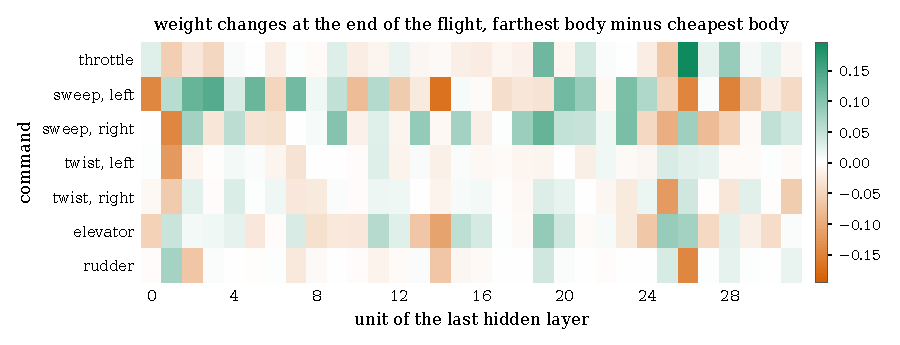
\includegraphics[width=\textwidth]{images/06_Results_and_Experiments/codesign/champion_deltaw.pdf}
\caption[Difference of the plastic weights on the two bodies]{Difference between the changes of the output weights, $\mat{W}_t - \mat{W}_0$ at the end of the flight, that the last set of rules of the run produces on the two bodies of \autoref{fig:champions}, flown on the same forest: one row per command, one column per unit of the last hidden layer, green where the farthest body's weight moved further up, orange where the cheapest body's did.}
\label{fig:champion-deltaw}
\end{figure}

The same rules do not do the same thing on the two bodies. \autoref{fig:champion-deltaw} compares the changes of the output weights at the end of a flight of each body under the best set of rules of the last generation of the run, on the same forest of the search kind, 630~m long, at a commanded speed of 12~m/s. The farthest body completes the forest in 54~s; the cheapest one flies 317~m and collides after 28~s. The two matrices of weight changes correlate at 0.76 over their 224 entries, and at 0.83 when the first is read at the same instant as the second ends. Where they differ, they differ most in the rows of the two sweep commands, by up to 0.20 where the trained weights have a mean magnitude of 0.05. This is one flight of each body and no more than an illustration. But it shows what \autoref{subsec:hebbian-why-output} asked of the plastic layer: the same rules, given a different body, arrive at different weights, and the difference is concentrated on the commands by which the two bodies differ most in what they can do.
% PROVENANCE: outer_exam_4_64_64_300_r0/.../plots/champion_videos/deltaw/deltaw_summary.csv (corr_final 0.7629, corr_matched 0.8260,
% max_abs_diff 0.1961, t 53.96 / 28.08 s, 630 m corridor seed 50, 12 m/s, controller_gen199_best_idx027).

\subsection{Generalization Capabilities of Evolved Controllers}
\label{subsec:results-generality}

The last question is what becomes of the rules. As \autoref{subsec:pipeline-run} anticipated, rules selected on bodies that resemble each other more at every update are asked to fly a family rather than anything, and \autoref{subsec:results-swapped-fronts} found that their gain in progress does not transfer to bodies of another front. Two measurements follow this along the run. The first is taken in every co-design run, at every generation, as described in \autoref{subsec:pipeline-run}. The best set of rules of the generation and the frozen generalist fly the reference drone, a body that is never in the population, on 4\,096 new forests of the search course. Over the first twenty generations the two differ by less than one point of fitness in all eight runs, in either direction. Over the last twenty generations the rules are below the frozen generalist by 10 to 16 points in all eight runs, flying 107 to 111~m of the course where the generalist flies 117~m. The loss grows monotonically along the run, and there is no early window in which the rules fly the reference drone better than the controller without rules.
% PROVENANCE: results/validation_summary.csv of the 8 co-design runs, best - baseline: first 20 gens -1.0..+0.4, last 20 gens -10.1..-16.1;
% progress last 20 gens 107.0..110.7 vs 116.7..116.8 m (computed 2026-09-29).

\begin{figure}[htbp]
\centering
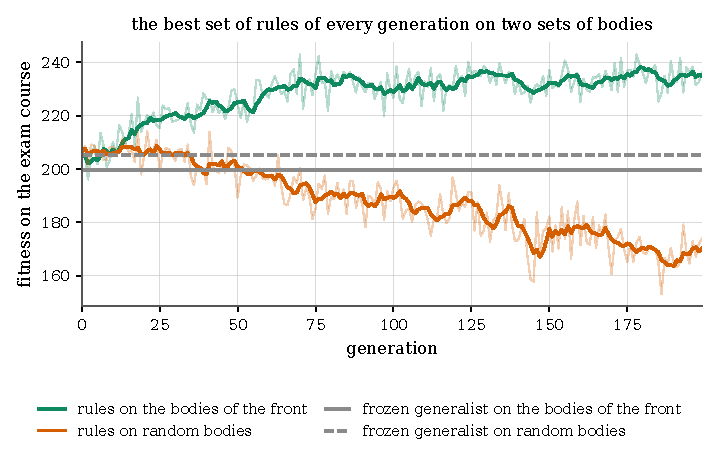
\includegraphics[width=0.8\textwidth]{images/06_Results_and_Experiments/codesign/generality_fitness.pdf}
\caption[The best set of rules of every generation on the bodies of the front and on random bodies]{The best set of rules of every generation of the first co-design run, flown on the 37 bodies of the run's last front (green) and on 128 bodies drawn at random from the design space (orange), over the same 64 forests of the exam course for every controller: fitness, mean over the bodies; thin lines are the raw values, thick lines a moving average over five generations. The grey lines are the frozen generalist on the same bodies and forests.}
\label{fig:generality}
\end{figure}

The second measurement asks the same question of the bodies the rules were selected for and of bodies they never met, on the same course as the exam (\autoref{fig:generality}). For the first co-design run, the best set of rules of each of the 200 generations was flown on the 37 bodies of the run's last front and on 128 bodies drawn at random from the design space, as the first population is. Every controller flew the same 64 forests of the exam course, next to the frozen generalist on the same bodies and forests. On the front bodies the rules of the first 25 generations already add 11 points of fitness and 8~m of progress to the frozen generalist. The gain grows to 29 points and 19~m by generations 50 to 74, and it levels off from generation 75 at 32 to 36 points and 22 to 25~m, 17\,\% of the fitness, with every one of the 37 bodies flying farther, while their cost of transport does not move. On the random bodies the same rules add 2 points in the first 25 generations, nothing that the 128 bodies can resolve, and they lose from then on without pause: 10 points by generations 50 to 74, 27 points by generations 125 to 149, and 37 points and 26~m of progress in the last 25 generations, an 18\,\% loss. Against this loss stands a saving of 0.01 to 0.02 in cost of transport, which is the portable economy of \autoref{subsec:results-swapped-fronts} once more.
% PROVENANCE: outer_exam_4_64_64_300_r0/.../generality/summary.csv (WP2_Outer_Loop.controller_generality, 2026-08-31): front n 37, random n 128,
% 64 exam forests, 201 controllers; block means recomputed 2026-09-29 (front +11.4/+29.2/+35.5, random +1.8/-10.4/-36.9 fitness).

The two curves are what specialization looks like. The gain on the bodies of the front saturates within the first half of the run, when the family of bodies has largely formed. The loss on bodies outside the front goes on to the last generation. The rules are therefore not simply degrading: they are following the bodies that the outer loop keeps, whose population narrows in the meantime from a mean pairwise distance of 1.56 in the genome cube at the first phase to 0.70 at the last. \emph{What the pipeline pays for its front is the generality of the controller it started from.} The rules that fly the evolved bodies 17\,\% better than the frozen generalist fly a random body 18\,\% worse and the reference drone 6 to 9\,\% worse. They could not be reused on another family of bodies without being evolved again, as \autoref{subsec:results-swapped-fronts} showed at the scale of a front. For the search this is not a defect. The controller was paid for once, as \autoref{sec:challenge-feasibility} required, and the adaptation of its output layer to the bodies being scored is what the rules provide at the cost of the flights. That the adaptation is to the family the search retains, rather than to every body in the space, is what makes it cheap.
% PROVENANCE: population diversity computed 2026-09-29 from outer_population.csv (first phase 1.55-1.57 in all 16 runs, last phase 0.69-0.95
% co-design, 0.75-0.92 morphology-only: the control narrows as much, so this is stated for the run of the figure only).

\subsection{Convergence or Plasticity?}
\label{subsec:results-convergence-plasticity}

\chapter{Conclusions \& Future Work}
\label{ch:conclusions}

\section{Conclusions}
\label{sec:conclusions}

This thesis asked whether a controller can adapt to the body it is given at a cost small enough to sit inside a search over bodies, and whether such an adaptation changes what the search finds. The shape of any answer was fixed in \autoref{ch:challenges}: a controller trained once for the whole space of bodies, and an adaptation to the body being scored that costs no more than the flights that score it. That shape was given a content in \autoref{ch:method}: a generalist trained by reinforcement learning and then frozen, Hebbian rules on its output layer evolved by CMA-ES, and a pipeline that nests the search of the rules inside a multi-objective search over the bodies. In \autoref{ch:results} the pipeline was run eight times against eight runs of the search under the frozen generalist, and the inner loop was isolated on fixed bodies. \emph{The experiments answer the question in the affirmative: an adaptation that costs no more than the flights that score a body changes the outcome of the search over bodies, and it changes that outcome for the better on both objectives.} The paragraphs that follow state what was found, in the order in which the thesis built it.

\paragraph{The adaptation costs no more than the flights.} The whole pipeline consists of flights of a network that is never trained again. A run of 200 generations flies about a quarter of a million flights per generation, examines 3\,136 bodies, of which at most 1\,600 are distinct, and takes about four days on one computing node with two graphics cards. The control condition, which updates its bodies at every generation and gives each body the same number of exam flights, took about 130 hours against 94. A controller training for each distinct body would have taken almost two months with a specialist trained for each body, and two and a half years with a controller of the generalist's kind. The cost of the adaptation is the cost of the flights, as the computational feasibility challenge required.

\paragraph{Co-design improves on morphology-only evolution on both objectives.} On the exam course the cumulative fronts of the two conditions agree at their two ends and separate in between. The tip of a front is common to both conditions: no body of either condition flies past 226~m of the 300~m course. The cheap arm of the front, the bodies that fly 85 to 110~m for a cost of transport of 0.10 to 0.12, is the same in both conditions. Between 128 and 213~m of progress the co-design fronts are cheaper at every level. At 150, 170 and 190~m the cheapest co-design body spends 16 to 17\,\% less energy per metre than the cheapest body of the control. Within a cost of transport of 0.15 to 0.25 the farthest co-design body flies 9 to 12\,\% farther. On each of these indicators every one of the eight co-design runs is better than every one of the eight control runs, and the hypervolume of the fronts separates the two groups as completely. The control was given more exams, more examined bodies and more computing time, and it did not catch up. The reference drone, a body of ordinary proportions, lies on the mean front of the control. At the progress of the reference drone the control finds bodies that are 4 to 6\,\% cheaper, and the co-design runs find bodies that are 18 to 23\,\% cheaper. \emph{The adaptation makes the search find bodies that spend less at equal progress and travel farther at equal cost of transport, and the margin over the reference drone is several times the margin that the search under the fixed controller obtains from the same starting bodies.}

\paragraph{The body search takes a different direction when the controller adapts.} Started from the same 64 bodies, the two conditions do not go to the same place in the space of the genome. Seven of the eight morphology-only runs end in one cluster, and the eighth ends elsewhere. Under a fixed controller the search over bodies has one main optimum, and most runs find it. The co-design runs end farther apart from each other, and farther from the cluster than the clustered control runs are from one another. A co-design run is no closer to the control run that started from its own bodies than to a control run that started from other bodies. This is the morphology optimization challenge observed in the data. \emph{An adapting controller does not shift the optimum of the body search by a fixed amount: it changes which bodies come first.} The two ends of one co-design front show how different the bodies that come first can be. One end is a light body of 0.58~kg with wing panels of 0.40~m and its centre of mass well aft, which flies 220~m at a cost of transport of 0.39. The other end is a glider of 1.96~kg with a wing of almost a square metre and its centre of mass forward, which flies 128~m at a cost of transport of 0.13. The two bodies share the gear ratios of their joints and a cambered airfoil: the run moved the wing and the fuselage, and kept the actuation.

\paragraph{The controller adapts to the morphology.} A co-design front is a front of pairs. Flown again under their own rules, the bodies of a co-design front travel 9 to 19~m farther than under the frozen generalist, and almost every body of every front travels farther. The same rules transplanted onto the bodies of a morphology-only front add 1 to 6~m. The progress that the rules add therefore belongs to the bodies they were evolved with, and those bodies were retained because the rules fly them. A co-design front is not the front of the generalist with a better controller on top. The weights that the rules produce depend on the body. The same set of rules, flown on the two bodies at the ends of a front, arrives at weight changes that differ most on the two sweep commands. The sweep is the command by which the two bodies differ most in what they can do. The rules are never told which body they fly. The body reaches them through the activity it induces in the frozen layers, and the rules turn that activity into gains that suit that body. \emph{This is adaptation to the body in the sense in which \autoref{sec:hebbian-controller} defined it: the same rules, given a different body, arrive at a different controller.}

\paragraph{The rules recover part of what the generalist lacks on a given body.} On the reference drone the frozen generalist scores 7.7 points of reward less than a specialist trained for that drone, a gap of 4\,\%. Rules evolved on that body recover 3.4 points, 44\,\% of the gap; measured against the three specialists that were trained, the recovery lies between a quarter and a half of the gap. The two gains are of a different kind. The advantage of the specialist lies in avoiding the trees. The specialist loses 28\,\% of its flights where the generalist loses 53\,\%, and it travels farther at a higher cost of transport. The rules leave the crashes and the progress where the generalist has them, and they lower the cost of transport by 9\,\% at a speed 3\,\% lower. In reward, the rules recover part of what the generalist lacks. In objective space, they move the body along the cost of transport at constant progress, an axis along which the specialist does not move. The same decomposition holds for rules evolved on 64 random bodies and measured on the reference drone, which that search never flew: a smaller gain, of the same kind.

\paragraph{On a specialist, the rules make the flight dynamics plastic.} Evolved on top of a specialist, the rules add more than anywhere else on a fixed body: 9.6 and 9.9 points on two of the three specialists, over 5\,\%, and nothing on the second. The frozen controllers explain the difference. The three specialists were trained with the same settings and different seeds, and they did not arrive at the same flight of the reference drone. The first and the third fly it at 13.9~m/s with a high cost of transport; the second flies it at 13.3~m/s and cheaply. Under their rules, all four base controllers, the generalist included, end at the same flight: 13.3 to 13.4~m/s, with crashes and progress untouched and a lower cost of transport. The second specialist was flying that flight already, and the rules leave it there. \emph{Where a base controller ends up under the rules does not depend on where it started, and what it gains is the distance it had to travel.} A specialist with rules is, in effect, a controller whose flight dynamics are plastic. The gains of its output layer, and with them the dynamics of the closed loop that the body forms with its controller, are retuned during the flight towards the flight that the fitness rewards on this body. The gain is real in the currency of the search, because a lower cost of transport at equal progress is a better point in objective space.

\paragraph{The price is the generality of the controller.} Along a run, the best rules of each generation fly the bodies of the final front better and better, up to 17\,\% more fitness than the frozen generalist, and they fly bodies drawn at random from the design space worse and worse, down to 18\,\% less. The reference drone, which is never in the population, ends 6 to 9\,\% worse under the rules than under the frozen generalist. The rules specialize to the family of bodies that the outer loop retains, and they could not be reused on another family without being evolved again. For the search this is not a defect. The search asked for an adaptation to the bodies being scored, and the adaptation to a family rather than to every body in the space is what keeps the adaptation cheap. For any other use of the evolved rules it is a limit.

\paragraph{Limits of the study.} Every quantity of this thesis was measured in simulation, with an aerodynamic model that is trusted for the order of the bodies rather than for absolute values. The tip of the fronts is the same in both conditions, so the comparison was made where the bodies had room to differ. The fixed-body gains were measured on one reference drone and on three specialists whose training reached different flights with the same settings, so that what the rules add to a controller depends on where that controller starts. One reward function was used as the fitness of the rules, and the economy that the rules find is the change that this reward pays for. The experiments say what an adaptation this cheap does inside this search. They do not say that evolved Hebbian rules are the best cheap adaptation, nor that the fronts found are the best fronts of the design space.

\emph{Within these limits, the thesis shows that a controller trained once and a few hundred evolved coefficients are enough to let a search over bodies find bodies that the adapted controller flies better than the fixed one. The results support the hypothesis that a search under the fixed controller would have discarded those bodies.}

\section{Future Work}
\label{sec:future-work}

Three directions follow from the results. The first concerns the representation on which the rules act, which this thesis left as the training produced it. The second and the third concern the transfer of the mechanism, to real drones and to systems other than drones.

\subsection{Meta-Learning Techniques}
\label{subsec:future-meta-learning}

The rules act on the latent representation of the last hidden layer. The frozen layers compute 32 features from the history of observations and commands, and the rules change only the gains that translate those features into the commands. The quality of the adaptation is therefore bounded by the quality of the representation. In this thesis the representation was trained by reinforcement learning for a controller with fixed gains, and nothing in that training anticipated that the gains would become plastic. The features are those that serve one compromise set of gains for all bodies, not those that would serve a set of gains adapted to each body. Gradient-based meta-learning trains representations for exactly this situation. MAML \cite{finn2017maml} learns an initialization from which a few gradient steps adapt a network to a new task. Raghu et al.\ \cite{raghu2020rapid} showed that adapting the last layer alone is enough when the features below are trained with that adaptation in the loop. If the bodies are read as tasks, the same procedure would train the features of the generalist so that an adaptation of the output layer to a body pays as much as possible. The Hebbian rules would then act on a representation built to be read by an adapted output layer. Two forms of this are possible. In the first, the features are meta-trained with gradient steps on the output layer over the training bodies, and the rules are evolved afterwards, as they are now. In the second, the rules of an earlier run are kept in place during the training of the generalist, so that the features are trained with the plastic output layer in the loop. The training of the features and the evolution of the rules then alternate. The second form resembles the co-training of differentiable plasticity \cite{miconi2018differentiable}, with the rules evolved instead of differentiated. \emph{The expected gain is in the half of the mechanism that this thesis kept fixed: the representation that the rules read.}

\subsection{Testing on Real Drones}
\label{subsec:future-real-drones}

The rules adapt the control to the body that is flying, read through the answer of that body to the commands. A real drone differs from its simulated model in its mass and inertia, in the aerodynamic forces on its surfaces and in the response of its servomotors. From the point of view of the rules, these differences are another body. The adaptation that the rules provide to a body they never met may therefore extend to the gap between simulation and reality, during flight and without a model of the discrepancy. The literature on evolved plastic networks gives reasons to expect this. Plastic controllers evolved in simulation transferred to a physical robot better than controllers with evolved fixed weights \cite{floreano2000evolutionary}. Shared Hebbian rules transferred to ten physical robots with a loss of under one percent \cite{vandiggelen2025emergent}. The base controller of this thesis was trained with the randomization of forces, masses and latencies on which transfer from simulation usually relies \cite{tobin2017domain, peng2018sim}. The rules would add an online adaptation to that offline robustness. None of this can be shown in simulation. The test requires that a body of a front, or the reference drone, be built with its morphing joints, that the network and the Hebbian update run on the onboard computer, and that the depth sectors be obtained from an onboard sensor. The computational part is within reach of any flight controller: the update of the 224 weights is a few thousand arithmetic operations per control step, at 25 steps per second. The laboratory where this work was carried out flies morphing winged drones of the same family \cite{bergonti2024codesign}, so the platform exists. \emph{Whether the rules close part of the gap between simulation and reality, leave it unchanged or widen it is a question that only a flight can answer.}

\subsection{Testing on Different Systems}
\label{subsec:future-other-systems}

The mechanism is general in what it requires: a network pretrained for a task over a family of conditions, a linear output layer, a stream of activity through that layer, and a quantity that varies between lifetimes and that the network is not told. Hebbian rules on top of a pretrained controller are, in this sense, a system-agnostic model. Within robotics, the body is not the only quantity of this kind. A payload, a worn actuator or a damaged limb change the dynamics in the same way, and the robustness to damage of evolved plastic networks is the result that made them known \cite{najarro2020meta}. Outside robotics, the same structure appears wherever a pretrained model follows a stream whose generating process changes between episodes. Sequence analysis is one case: a model trained on many sources is applied to a new source, with no labels on which to fine-tune it. The analysis of stochastic processes is another: the parameters of the process are fixed within an episode, hidden from the model and different from one episode to the next. This is the situation that this thesis described for the body. Differentiable plasticity has been applied to memorization and few-shot classification \cite{miconi2018differentiable}, so plastic weights can act on tasks of that kind. The open question is whether evolved rules on top of a frozen pretrained model give there the gain they gave here. The experiments of this thesis also say what to measure. \emph{The gain found here was a specialization to the family that the search retained, not a general improvement, so the measurement in any new system must be made both on the family and outside it.}

\printbibliography

\appendix
\chapter{Simulation Details}
\label{app:simulation}

This appendix collects the parts of the simulation that \autoref{ch:environment} summarizes: the internal organization of Genesis, the equations of its rigid body solver, the aerodynamic model in full, the formula of the aerodynamic noise, the collision test and the statistics of the forests, and the mass and power models of the drone. It documents the simulator as it was used in every experiment of this thesis.

\section{Genesis Architecture and Taichi Kernels}
\label{app:genesis-architecture}

A Genesis program builds a \emph{scene}. The scene owns a \emph{simulator}, and the simulator owns a set of \emph{solvers}, one for each physical model the engine supports: articulated rigid bodies, and a family of continuum models for liquids, granular media, cloth and deformable solids (the material point method, smoothed particle hydrodynamics, finite elements, position based dynamics and a grid based fluid solver). A \emph{coupler} exchanges forces between solvers when objects of different kinds touch. The objects themselves are \emph{entities}, each defined by a \emph{morph} that gives its geometry (a primitive shape, a mesh, or a robot description file) and by a material that decides which solver is responsible for it. Only the solvers that own at least one entity are stepped. In this thesis the scene contains a single entity, the drone, loaded from a Unified Robot Description Format (URDF) file that is generated from the genome of the body; it is handled by the rigid body solver, and the aerodynamic solver acts on it as one more solver of the same simulator. Rendering is a separate subsystem and stays switched off during training and search.

None of the numerical work is done by the Python interpreter. Genesis is built on \emph{Taichi} \cite{hu2019taichi, hu2020difftaichi}, a domain specific language for parallel numerical computation that is embedded in Python, and of which the Genesis developers maintain their own fork. A Taichi \emph{kernel} is a function written in a statically typed subset of Python syntax and marked with a decorator. The first time a kernel is called, Taichi does not execute its body: it reads the syntax tree of the function, translates it into its own intermediate representation, applies the usual optimizations of a compiler (constant folding, elimination of common subexpressions and of dead branches, simplification of memory accesses) and lowers the result through LLVM to machine code for the selected backend, which here is CUDA. This is \emph{just-in-time} compilation: the program is compiled while it runs, the first time each piece is needed, and every later call launches the compiled binary directly (\autoref{fig:taichi-kernel}).

\begin{figure}[htbp]
\centering
\begin{tikzpicture}[
    >={Stealth[length=2mm]}, thick,
    every node/.style={font=\small},
    node distance=0.55cm,
]
\node[agentbox, align=center] (py) {Python function\\marked as kernel};
\node[affbox, align=center, right=1.5cm of py] (ast) {syntax\\tree};
\node[affbox, align=center, right=0.45cm of ast] (ir) {Taichi IR,\\optimization};
\node[affbox, align=center, right=0.45cm of ir] (llvm) {LLVM};
\node[envbox, align=center, right=0.45cm of llvm] (bin) {GPU\\binary};
\node[concatbox, align=center, above=0.7cm of bin] (cache) {on-disk cache};
\node[criticbox, align=center, below=1.2cm of ir, xshift=0.2cm] (launch) {launch: one GPU thread for each\\iteration of the outermost loop};

\draw[->] (py) -- node[above]{\scriptsize first call} (ast);
\draw[->] (ast) -- (ir);
\draw[->] (ir) -- (llvm);
\draw[->] (llvm) -- (bin);
\draw[<->] (bin) -- (cache);
\draw[->] (bin.south) |- (launch.east);
\draw[->] (py.south) |- node[above, pos=0.72]{\scriptsize later calls} (launch.west);
\end{tikzpicture}
\caption[Life of a Taichi kernel]{Life of a Taichi kernel. The first call compiles the Python function down to a GPU binary, which is also written to a cache on disk; later calls, and later runs of the same program, skip the compilation and only launch the binary. IR stands for intermediate representation.}
\label{fig:taichi-kernel}
\end{figure}

What makes a kernel parallel is a single rule: the outermost \texttt{for} loop of a kernel is parallelized automatically, and on a GPU every iteration of that loop becomes one thread. The body of the loop can be arbitrary scalar code, with branches, local variables, inner loops and calls to other Taichi functions, and all of it is fused into one GPU program. This is the opposite of the way a tensor library such as PyTorch reaches the GPU, where every elementary operation is a separate GPU program that reads and writes whole arrays. Physics code is full of logic that differs from element to element (a joint limit that is active in one copy of the scene and not in the next, a wing that is stalled here and not there), and it is awkward and wasteful to express as a chain of whole-array operations, while inside a kernel it is an ordinary \texttt{if}. Every kernel launch from Python has a small fixed cost, so the engine is organized as a few large kernels rather than many small ones.

The data that kernels work on live in \emph{fields}: typed, multidimensional arrays that are allocated on the GPU and declared separately from the kernels that use them. Keeping the description of the data apart from the computation is the central idea of Taichi \cite{hu2019taichi}, and it has a consequence that matters in practice. A kernel refers to its fields as global variables, so at compilation time it is bound to those specific fields and to their shapes; and the parameters that are declared static (the options of a solver, the number of links of a robot, which branches of the code are enabled) are compiled in as constants, with the unused branches removed. A compiled kernel is therefore specialized to one scene. Genesis makes this explicit by separating the construction of a scene from its \emph{build}: entities and options are declared first, and a single build call then allocates every field and fixes every static parameter. After the build, the values stored in the fields can change freely, which covers the state of the simulation and the physical parameters that were declared as varying, but nothing structural can: not the number of bodies, not their topology or geometry, not the size of any array. A structural change requires a new scene and a new build.

The most important structural parameter is the number of parallel \emph{environments} $B$, given to the build call. The $B$ environments are independent copies of the scene that share one model (the kinematic tree, the geometry, the nominal inertias) and differ in their state. Every state field has an axis of length $B$: the generalized positions form an array of size $n_q \times B$, the joint space inertia matrix an array of size $n_v \times n_v \times B$, and the parallel loop of each kernel runs over pairs (element, environment), so that a single launch advances every link of every environment. Environments never interact, which is exactly the structure of the workloads of this thesis: many flights of the same body, each in its own forest. Finally, the fields can be read and written as PyTorch tensors that reside on the same GPU: the exchange is a copy between two regions of the memory of the card and never passes through the host. The neural controllers, the obstacle fields and the reward computations are PyTorch code, the physics is Taichi code, and during a run only logging scalars ever leave the GPU.

\section{Rigid Body Dynamics}
\label{app:rigid-body}

The drone is an articulated rigid body: a fuselage that moves freely in space and carries six revolute joints, driven by servomotors, which sweep and twist the two front wings and deflect the elevator and the rudder (the body is described in \autoref{sec:drone-model}). Its configuration $\vect{q}$ collects the position of the fuselage, its orientation as a unit quaternion and the six joint angles, for $n_q = 13$ numbers, and its generalized velocity $\vect{v}$ collects the linear and angular velocity of the fuselage and the six joint rates, for $n_v = 12$ degrees of freedom. The rigid body solver of Genesis follows the formulation of MuJoCo \cite{todorov2012mujoco}, and advances the equation of motion in generalized coordinates,
\begin{equation}
\mat{M}(\vect{q})\,\dot{\vect{v}} + \vect{c}(\vect{q}, \vect{v}) = \vect{\tau}_{\mathrm{act}} + \vect{\tau}_{\mathrm{pas}} + \mat{J}_{\mathrm{a}}(\vect{q})^{\top} \vect{F}_{\mathrm{a}} + \mat{J}_{\mathrm{c}}(\vect{q})^{\top} \vect{f}_{\mathrm{c}},
\label{eq:eom}
\end{equation}
where $\mat{M}$ is the joint space inertia matrix, $\vect{c}$ gathers the Coriolis, centrifugal and gravitational terms, $\vect{\tau}_{\mathrm{act}}$ and $\vect{\tau}_{\mathrm{pas}}$ are the actuator and the passive joint torques, $\vect{F}_{\mathrm{a}}$ stacks the aerodynamic forces with $\mat{J}_{\mathrm{a}}$ the Jacobian of their points of application, and $\vect{f}_{\mathrm{c}}$ are the constraint forces with Jacobian $\mat{J}_{\mathrm{c}}$. At every substep the solver computes $\mat{M}$ with the composite rigid body algorithm and $\vect{c}$ with the recursive Newton-Euler algorithm \cite{featherstone2008rigid}, both of which traverse the kinematic tree in a time linear in the number of links, and factorizes $\mat{M}$ once for all the linear systems that follow.

The servomotors are modelled as proportional-derivative position controllers with a bounded torque,
\begin{equation}
\tau_{\mathrm{act},j} = \operatorname{clip}\!\left( k_p \left(q_j^{\star} - q_j\right) - k_v\, v_j,\; -\tau_j^{\max},\; \tau_j^{\max} \right),
\label{eq:servo}
\end{equation}
with $k_p = 8$~N\,m/rad, $k_v = 2$~N\,m\,s/rad and a torque limit of 1~N\,m for the tail joints. The servomotors of the wing have a fixed limit of their own, and what reaches the joint is that limit multiplied by the gear ratio of the body (\autoref{subsec:drone-shape}): 1.5~N\,m on the reference drone. The target angle $q_j^{\star}$ is what the controller commands. The passive torques are a viscous damping and a dry friction in each joint, and an armature term, which stands for the reflected inertia of the motor and of its gears, is added to the diagonal of $\mat{M}$. The response of a control surface to a command is thus not instantaneous: it is the response of a damped second order system with a saturating motor, and its delay is part of what the controller has to cope with.

Constraints are handled as in MuJoCo, by a convex optimization over accelerations rather than by a complementarity problem \cite{todorov2014convex}. Let $\vect{a}_0 = \mat{M}^{-1}(\vect{\tau}_{\mathrm{act}} + \vect{\tau}_{\mathrm{pas}} + \mat{J}_{\mathrm{a}}^{\top} \vect{F}_{\mathrm{a}} - \vect{c})$ be the acceleration the system would have without constraints. The solver selects
\begin{equation}
\begin{gathered}
\dot{\vect{v}} = \arg\min_{\vect{a}}\; \frac{1}{2}\,(\vect{a} - \vect{a}_0)^{\top} \mat{M}\, (\vect{a} - \vect{a}_0) \;+\; \sum_{i \,\in\, \mathcal{A}(\vect{a})} \frac{1}{2}\, d_i \left( \mat{J}_i\, \vect{a} - a_i^{\mathrm{ref}} \right)^2, \\
a_i^{\mathrm{ref}} = -b_i\, \mat{J}_i \vect{v} - k_i\, r_i ,
\end{gathered}
\label{eq:constraint-opt}
\end{equation}
that is, the acceleration closest to the unconstrained one in the metric of the kinetic energy (Gauss's principle of least constraint), softened by a penalty on each active constraint $i$. The reference acceleration $a_i^{\mathrm{ref}}$ is that of a critically damped spring which would bring the violation $r_i$ back to zero within a chosen time constant, the weight $d_i$ sets how stiffly the constraint is enforced, and the set $\mathcal{A}(\vect{a})$ contains the inequality constraints that are currently pushing in their admissible direction. The problem is convex and has a unique solution, and the constraint forces $\vect{f}_{\mathrm{c}}$ follow from it. Genesis offers a Newton and a conjugate gradient method for \eqref{eq:constraint-opt}; this thesis uses the latter. In the scenes of this work the problem is small, because contacts are disabled (see below): the only constraints are the mechanical limits of the six joints, which become active only when a joint reaches its stop, and the dry friction of the joints.

Time integration is semi-implicit Euler. With substep $\Delta t$,
\begin{equation}
\vect{v}_{k+1} = \vect{v}_k + \Delta t\, \dot{\vect{v}}_k, \qquad \vect{q}_{k+1} = \vect{q}_k \oplus \Delta t\, \vect{v}_{k+1},
\label{eq:integration}
\end{equation}
where the new velocity is used to advance the positions and $\oplus$ denotes ordinary addition for positions and joint angles and the composition with the rotation of axis and angle $\Delta t\,\vect{\omega}_{k+1}$ for the quaternion, which thereby stays of unit norm. The default integrator of Genesis, used here, makes one modification for stiff actuators: the joint damping $\mat{D}$ and the derivative gains $\mat{K}_v$ of the servomotors are treated implicitly, which amounts to replacing $\mat{M}$ with $\mat{M} + \Delta t\,(\mat{D} + \mat{K}_v)$ in the computation of the acceleration and keeps the servo loop stable whatever its gains. All other forces, the aerodynamic ones included, are explicit: they are evaluated on the state at the beginning of the substep and held constant across it.

Genesis has a complete collision pipeline: a broad phase that sorts axis-aligned bounding boxes to discard distant pairs, a narrow phase for convex shapes, a convex decomposition for meshes that are not convex, and contact forces with Coulomb friction that enter \eqref{eq:constraint-opt} as further constraints. None of it is used here, and the trees of the forest are not objects of the physics engine at all. There are two reasons. A flight ends the moment the drone touches anything, so no contact ever has to be resolved, only detected. And the geometry of a scene is shared by all of its environments, whereas this work needs a different random forest in every environment. The forests are therefore stored outside the engine, as tensors that hold the position of every trunk in every environment, and the two operations that involve them, the depth sensing of the drone and the detection of a collision, are computed geometrically on those tensors for all environments at once (\autoref{sec:flight-environment}). Likewise there is no ground plane: a flight that descends below a minimum altitude is ended.

\section{Aerodynamic Model}
\label{app:aero}

The model below is the one credited in \autoref{subsec:genesis-aero}, documented as it was used.

The aerodynamic solver computes, at every physics substep and for every environment, the force that the air exerts on each part of the drone, and hands these forces to the rigid body solver as the term $\mat{J}_{\mathrm{a}}^{\top} \vect{F}_{\mathrm{a}}$ of \eqref{eq:eom}. It is a \emph{quasi-steady component build-up}: the aircraft is divided into a small number of elements, each element receives one lumped force that depends only on the instantaneous flow it sees, through lift and drag coefficients of closed form, and the forces are summed by the rigid body dynamics. A model of this kind is orders of magnitude cheaper than any solution of the flow field, which is what allows it to run a hundred times per simulated second in a quarter of a million environments. It is also algebraic in the geometry of the body, so that a new body needs no aerodynamic data of its own: areas, chords, spans and aspect ratios are read from the same URDF file that defines the rigid body, and the coefficients follow from them.

\paragraph{Elements and local flow.} The drone has seven aerodynamic elements: the fuselage, the two halves of the wing, the two halves of the elevator, the rudder and the propeller. Each lifting surface carries a reference frame at the quarter of its chord, with the $x$ axis along the chord towards the trailing edge, the $y$ axis along the span and the $z$ axis normal to the surface. The frame is rigidly attached to the link of the surface and moves with it, and this is how the morphing of the wing enters the aerodynamics without any dedicated model: a twist of a wing half pitches its frame and changes its angle of attack, a sweep yaws the frame, changes its sideslip and displaces its point of application. The air is assumed at rest. If $\vect{v}_{\mathrm{cm}}$ is the velocity of the centre of mass of the drone and $\mat{R}_i$ the orientation of the frame of element $i$, the relative wind seen by the element and its aerodynamic angles are
\begin{equation}
\begin{gathered}
\vect{w}_i = -\mat{R}_i^{\top} \vect{v}_{\mathrm{cm}}, \qquad V_i = \lVert \vect{w}_i \rVert, \\
\alpha_i = \operatorname{atan2}\!\left(w_{i,z},\, w_{i,x}\right), \qquad \beta_i = \arcsin\frac{w_{i,y}}{V_i},
\end{gathered}
\label{eq:aero-angles}
\end{equation}
the angle of attack $\alpha_i$ and the sideslip angle $\beta_i$. The index $i$ is dropped in what follows.

\paragraph{Lift and drag coefficients.} For small angles of attack a lifting surface behaves according to the classical theory of the finite wing \cite{anderson2017fundamentals}. The slope of its lift curve is lower than that of its airfoil section, $C_{\ell_\alpha}$, because the vortices shed at the tips reduce the effective incidence, and the reduction grows as the aspect ratio $\mathit{AR}$ of the surface decreases. The solver uses the formula of Helmbold, which unlike the better known lifting-line result remains accurate for the low aspect ratios of a small drone:
\begin{equation}
C_{L_\alpha} = C_{\ell_\alpha}\, \frac{\mathit{AR}}{2 + \sqrt{\mathit{AR}^2 + 4}} .
\label{eq:helmbold}
\end{equation}
Lift is linear in the angle of attack measured from the zero-lift angle $\alpha_0$ of the section, and drag is the sum of a parasitic part and of the drag induced by lift:
\begin{equation}
C_L^{\mathrm{lin}} = f_{\mathit{Re}}\; C_{L_\alpha}\,(\alpha - \alpha_0), \qquad
C_D^{\mathrm{lin}} = C_{D_0} + \frac{\left(C_L^{\mathrm{lin}}\right)^2}{\pi\, e\, \mathit{AR}},
\label{eq:aero-linear}
\end{equation}
with $e = 0.8$ the Oswald efficiency factor. The factor $f_{\mathit{Re}} = \min(\mathit{Re}/\mathit{Re}_{\mathrm{nom}},\, 1)$, where $\mathit{Re} = \rho V \bar c/\mu$ is the Reynolds number of the surface computed on its mean chord $\bar c$, reduces the lift of a surface that operates below the nominal Reynolds number of its section, as happens to a narrow wing in slow flight. The aspect ratio in \eqref{eq:helmbold} and \eqref{eq:aero-linear} is that of the complete wing, including the part of the span covered by the fuselage, with the span reduced by the factor $\cos\beta$ when the surface is swept or the drone flies with sideslip.

The linear regime ends at stall, and a controller that manoeuvres among obstacles, or a body that is badly proportioned, will cross it; a model that stops at stall would make every such event a numerical accident. Beyond stall the solver therefore switches to the coefficients of a flat plate in fully separated flow,
\begin{equation}
C_L^{\mathrm{fp}} = f_{\mathit{Re}}\, \sin 2\alpha, \qquad C_D^{\mathrm{fp}} = 2\, f_{\mathit{Re}}\, \sin^2\!\alpha ,
\label{eq:aero-plate}
\end{equation}
which are defined for any incidence, reversed flow included, and give the correct limits: no lift and the drag of a plate normal to the wind at $\alpha = 90^{\circ}$. The two regimes are joined by a smooth switch centred on the stall angle $\alpha_s$, as is common in the flight dynamics models of small unmanned aircraft \cite{beard2012small}:
\begin{equation}
\begin{gathered}
\sigma(\alpha) = \frac{1}{2}\left[ 1 + \tanh\frac{\lvert\alpha\rvert - \alpha_s}{m\,\alpha_s} \right], \\
C_L = (1-\sigma)\, C_L^{\mathrm{lin}} + \sigma\, C_L^{\mathrm{fp}}, \qquad
C_D = (1-\sigma)\, C_D^{\mathrm{lin}} + \sigma\, C_D^{\mathrm{fp}},
\end{gathered}
\label{eq:aero-blend}
\end{equation}
with $m = 0.2$ the relative width of the transition. A finite wing stalls at a larger angle than its section, because it needs more incidence to reach the same lift. The solver accounts for this by computing the stall angle of the surface from that of the section, $\alpha_s^{\mathrm{2D}}$:
\begin{equation}
\alpha_s = \alpha_0 + \frac{2\pi\,\delta}{C_{L_\alpha}\left(1 + 2\delta/\mathit{AR}\right)}, \qquad \delta = \alpha_s^{\mathrm{2D}} - \alpha_0 .
\label{eq:aero-stall}
\end{equation}
The numerator is the maximum lift coefficient that thin airfoil theory assigns to the section, and the division by $C_{L_\alpha}$ gives the incidence at which the finite surface reaches it; the term in brackets is an empirical correction that lowers the result for short wings. The correction is applied to the wing and to the elevator, while the rudder keeps the stall angle of its section. \autoref{fig:aero-coefficients} shows the resulting curves for the wing of the reference drone.

\begin{figure}[htbp]
\centering
\begin{tikzpicture}[x=0.125cm, y=2.3cm, thick, every node/.style={font=\small}]
% axes
\draw[->, thin] (-12,0) -- (95,0) node[right]{$\alpha$};
\draw[->, thin] (0,-0.55) -- (0,2.2);
\foreach \a in {-10,10,20,30,40,50,60,70,80,90} {
    \draw[thin] (\a,0.03) -- (\a,-0.03) node[below, font=\scriptsize]{$\a^{\circ}$};
}
\foreach \v in {-0.5,0.5,1.0,1.5,2.0} {
    \draw[thin] (0.8,\v) -- (-0.8,\v) node[left, font=\scriptsize]{\v};
}
% stall angle
\draw[thin, dash dot, gray!60!black] (12.0,-0.1) -- (12.0,2.1) node[above, font=\scriptsize, text=black]{$\alpha_s$};
% linear and flat plate models
\draw[thin, dashed, blue!60!black] (-10,-0.590) -- (20,1.945);
\draw[semithick, densely dotted, blue!60!black] plot[smooth] coordinates {(-10,-0.342) (-5,-0.174) (0,0.000) (5,0.174) (10,0.342) (15,0.500) (20,0.643) (25,0.766) (30,0.866) (35,0.940) (40,0.985) (45,1.000)};
\draw[semithick, densely dotted, red!65!black] plot[smooth] coordinates {(-10,0.060) (-5,0.015) (0,0.000) (5,0.015) (10,0.060) (15,0.134) (20,0.234) (25,0.357) (30,0.500)};
% CL
\draw[very thick, blue!70!black] plot[smooth] coordinates {(-10,-0.551) (-9,-0.491) (-8,-0.416) (-7,-0.335) (-6,-0.252) (-5,-0.168) (-4,-0.083) (-3,0.001) (-2,0.086) (-1,0.170) (0,0.255) (1,0.339) (2,0.424) (3,0.508) (4,0.592) (5,0.676) (6,0.758) (7,0.837) (8,0.908) (9,0.962) (10,0.980) (11,0.939) (12,0.838) (13,0.716) (14,0.623) (15,0.578) (16,0.567) (17,0.576) (18,0.596) (19,0.619) (20,0.644) (21,0.670) (22,0.695) (23,0.719) (24,0.743) (25,0.766) (26,0.788) (27,0.809) (28,0.829) (29,0.848) (30,0.866) (33,0.914) (36,0.951) (39,0.978) (42,0.995) (45,1.000) (48,0.995) (51,0.978) (54,0.951) (57,0.914) (60,0.866) (63,0.809) (66,0.743) (69,0.669) (72,0.588) (75,0.500) (78,0.407) (81,0.309) (84,0.208) (87,0.105) (90,0.000)};
% CD
\draw[very thick, red!70!black] plot[smooth] coordinates {(-10,0.036) (-8,0.023) (-6,0.017) (-4,0.014) (-2,0.014) (0,0.017) (2,0.023) (4,0.032) (6,0.044) (8,0.059) (10,0.075) (12,0.093) (14,0.118) (16,0.152) (18,0.191) (20,0.234) (22,0.281) (24,0.331) (26,0.384) (28,0.441) (30,0.500) (33,0.593) (36,0.691) (39,0.792) (42,0.895) (45,1.000) (48,1.105) (51,1.208) (54,1.309) (57,1.407) (60,1.500) (63,1.588) (66,1.669) (69,1.743) (72,1.809) (75,1.866) (78,1.914) (81,1.951) (84,1.978) (87,1.995) (90,2.000)};
\node[blue!70!black, font=\small] at (52,0.78) {$C_L$};
\node[red!70!black, font=\small] at (75,1.66) {$C_D$};
% legend
\draw[very thick, black!70] (35,2.08) -- (41,2.08) node[right, font=\scriptsize, text=black]{blended model};
\draw[thin, dashed, black!70] (35,1.93) -- (41,1.93) node[right, font=\scriptsize, text=black]{linear model};
\draw[semithick, densely dotted, black!70] (35,1.78) -- (41,1.78) node[right, font=\scriptsize, text=black]{flat plate model};
\end{tikzpicture}
\caption[Lift and drag coefficients of the aerodynamic model]{Lift and drag coefficients of the aerodynamic model for the wing of the reference drone (NACA 3416 section, aspect ratio 7.5). The dashed line is the linear model \eqref{eq:aero-linear} (shown for the lift only), the dotted lines are the flat plate model \eqref{eq:aero-plate}, and the solid lines are their blend \eqref{eq:aero-blend} around the stall angle $\alpha_s = 12.0^{\circ}$ of the finite wing. The maximum lift coefficient is 0.98 and the best lift to drag ratio of the isolated wing is 18.7.}
\label{fig:aero-coefficients}
\end{figure}

The parameters of the section, $\alpha_0$, $\alpha_s^{\mathrm{2D}}$, $C_{D_0}$ and $\mathit{Re}_{\mathrm{nom}}$, are not free constants. The wing section is a four-digit NACA airfoil chosen by the genome of the body, and its parameters are read from a table that was computed in advance, for every admissible airfoil, from polars obtained with the panel code XFOIL \cite{drela1989xfoil} over a sweep of Reynolds numbers. The slope of the section is fixed at $C_{\ell_\alpha} = 0.11$ per degree, the value that thin airfoil theory predicts to within one percent. The elevator and the rudder always use the same symmetric section. The fuselage produces no lift and a constant drag coefficient of 0.35 referred to its own reference area.

\paragraph{Forces and points of application.} With the dynamic pressure $\tfrac{1}{2}\rho V^2$, the air density $\rho = 1.225$~kg/m$^3$ and the area $S$ of the element, lift and drag are
\begin{equation}
L = \tfrac{1}{2}\,\rho V^2 S\, C_L \cos^2\!\beta, \qquad D = \tfrac{1}{2}\,\rho V^2 S\, C_D \cos^2\!\beta,
\label{eq:aero-lift-drag}
\end{equation}
where the factor $\cos^2\beta$, applied to the wing and to the elevator, expresses the classical result that only the component of the flow normal to the span of a surface loads it. The two magnitudes are assembled in wind axes and rotated into the frame of the surface through the two aerodynamic angles,
\begin{equation}
\vect{F} = \mat{R}_z(\beta)\, \mat{R}_y(\alpha)\, \bigl( D,\; 0,\; L \bigr)^{\top},
\label{eq:aero-force}
\end{equation}
with $\mat{R}_y$ and $\mat{R}_z$ the elementary rotations about the $y$ and $z$ axes of the frame. The rudder is treated as a wing turned by ninety degrees: its incidence is the sideslip angle, its coefficients are evaluated at $\beta$, and its lift acts as a side force along $y$. The force is not applied at the origin of the frame but at the \emph{centre of pressure} of the surface, which for an attached flow lies at the quarter of the chord and moves towards the middle of the chord as the flow separates:
\begin{equation}
\frac{x_{\mathrm{cp}}}{\bar c} = \frac{1}{4} + \frac{1}{4}\, \frac{\lvert\alpha\rvert}{\pi/2} .
\label{eq:aero-cp}
\end{equation}
Since the rigid body solver receives a force and a point, the aerodynamic moments of the drone are never modelled as such: the pitching moment that trims the aircraft, the rolling moment of a differential twist and the yawing moment of an asymmetric sweep all arise as moments of the forces \eqref{eq:aero-force} about the centre of mass, and they change with the body because the points of application do.

\paragraph{Interaction between the elements.} Two interactions are modelled, both directed at the tail. The first is the \emph{downwash} of the wing: a wing that produces lift deflects the flow behind it downwards, and the elevator works in that deflected flow. Its angle of attack is reduced by the downwash angle that lifting-line theory predicts at the wing,
\begin{equation}
\alpha_{\mathrm{t}} = \alpha - \varepsilon, \qquad \varepsilon = k_{\varepsilon}\, \frac{C_{L,\mathrm{w}}}{\pi\, \mathit{AR}_{\mathrm{w}}},
\label{eq:aero-downwash}
\end{equation}
where $C_{L,\mathrm{w}}$ is the lift coefficient that the wing half on the same side has at that same substep, $\mathit{AR}_{\mathrm{w}}$ the aspect ratio of the wing and $k_{\varepsilon} = 1$. This couples the two surfaces the way it does on a real aircraft (an increase of wing lift reduces the effectiveness of the tail) and makes the two halves of the elevator work differently when the two halves of the wing do. For this reason the kernel evaluates the elements in a fixed order: the propeller first, then the wing and the fuselage, then the tail. The second interaction is the \emph{slipstream} of the propeller, whose induced velocity, given below, corrects the axial component of the flow seen by the elevator through a gain $k_s$.

\paragraph{Propeller.} The throttle command $u \in [0,1]$ does not set the thrust directly. It passes through a first order lag that represents the inertia of the motor and of the propeller,
\begin{equation}
\tilde u_{k+1} = \tilde u_k + \frac{\Delta t}{\Delta t + 1/(2\pi f_c)}\,\left(u_k - \tilde u_k\right),
\label{eq:prop-lag}
\end{equation}
with a cut-off frequency $f_c = 0.32$~Hz, and the filtered command sets the rotation speed $n = \tilde u\, n_{\max}$ (in revolutions per second), where $n_{\max}$ is the smaller of the no-load speed of the motor, $K_V U / 60$ for a speed constant $K_V = 2300$~rpm/V and a supply voltage $U = 7.4$~V, and of the speed at which the propeller delivers its maximum static thrust $T_{\max} = 5.2$~N. The thrust of a propeller of diameter $d$ falls as the aircraft flies faster, because the blades meet the air at a lower incidence; this is described by a thrust coefficient that decreases with the \emph{advance ratio} $J$ \cite{mccormick1995aerodynamics}:
\begin{equation}
J = \frac{V_a}{n\, d}, \qquad T = \rho\, n^2 d^4\, C_{T_0} \max\!\left(0,\; 1 - c_1 J - c_2 J^2\right),
\label{eq:prop-thrust}
\end{equation}
with $V_a$ the component of the relative wind along the axis of the propeller, $C_{T_0} = 0.093$, $c_1 = 0$ and $c_2 = 2.148$, and $T$ limited to the interval $[0, T_{\max}]$. The thrust acts along the axis, together with a reaction torque $\kappa T$ about it, $\kappa = 0.01$~m. The velocity induced in the slipstream follows from the momentum theory of the actuator disc of area $A = \pi d^2/4$:
\begin{equation}
v_{\mathrm{ind}} = \frac{1}{2}\left( -V_a + \sqrt{V_a^2 + \frac{2T}{\rho A}} \right).
\label{eq:prop-induced}
\end{equation}
The dependence of the thrust on the flight speed matters for the two objectives of this thesis. A model with a thrust proportional to the throttle would make fast flight as cheap as slow flight; with \eqref{eq:prop-thrust} the propeller loses effectiveness with speed, and the energy spent per metre depends on how well the drag of the body matches the propeller over the range of speeds at which the controller is commanded to fly.

\paragraph{Coupling and safeguards.} At each substep the forces of all elements, with their points of application, are transformed to the world frame and accumulated on the links of the rigid body as forces and moments. Three safeguards protect the explicit coupling. The speed $V$ that enters the coefficients is limited to 40~m/s, the force on each element is limited to 30~N, several times the weight of the drone, and values that are not finite are replaced by zero before they reach the rigid body solver. In a parallel simulation this last point is not cosmetic: the environments of a scene are advanced by the same kernels on shared arrays, and a single environment whose state diverges can otherwise spread its invalid values to the rest of the batch.

\paragraph{Limits of the model.} The model is a compromise between fidelity and the cost of evaluating it a hundred times per second in every environment, and its simplifications should be stated. It is quasi-steady: forces depend on the instantaneous flow only, so unsteady effects such as dynamic stall or the lag of the downwash in reaching the tail are absent. Each surface carries a single lumped force, so the distribution of the load along the span, and with it the progressive stall of a twisted or swept wing, is not resolved. The relative wind \eqref{eq:aero-angles} of every element is computed from the velocity of the centre of mass: the additional flow that a rotation of the body induces at a surface far from the centre of mass is neglected, and the rotations of the drone are damped only indirectly, through the change of incidence they produce. Interference is limited to the two effects described above. Finally, the air is at rest: there is no wind and no turbulence other than the noise described in \autoref{app:aero-noise}. None of this prevents the model from ranking bodies by the quantities that drive the search (how much wing a body has, how it is proportioned, where its surfaces sit with respect to its centre of mass, which section it uses), but the absolute values of range and energy it produces are those of the model and would need to be validated against flight data before being read as predictions.

\section{Aerodynamic Noise}
\label{app:aero-noise}

The first of the three levels of noise described in \autoref{subsec:genesis-noise} is the aerodynamic force itself. At every physics substep, and independently for every lifting surface of every environment, the force \eqref{eq:aero-force} is perturbed in magnitude and in direction before it is applied:
\begin{equation}
\begin{gathered}
\tilde{\vect{F}} = \lVert \vect{F} \rVert \left(1 + \sigma_m\, s\, \xi\right) \frac{\hat{\vect{F}} + \sigma_d\, s\, \vect{g}_{\perp}}{\lVert \hat{\vect{F}} + \sigma_d\, s\, \vect{g}_{\perp} \rVert}, \\
s(\alpha, \beta) = 1 + 3 \left( \frac{\min\!\left(\sqrt{\alpha^2 + \beta^2},\, \pi\right)}{\pi} \right)^{\!2},
\end{gathered}
\label{eq:aero-noise}
\end{equation}
where $\hat{\vect{F}}$ is the unit vector of $\vect{F}$, $\xi$ a standard normal variable, $\vect{g}_{\perp}$ a random unit vector orthogonal to $\vect{F}$, and $\sigma_m = \sigma_d = 0.05$. The scale $s$ grows from 1 in aligned flow to 4 in fully reversed flow, so that the force is least reliable exactly where the model is: at large incidence, around and beyond stall. The centre of pressure is displaced at the same time by a random offset whose standard deviation is a fraction $\sigma_{\mathrm{cp}}\, s / 4$ of the chord, with $\sigma_{\mathrm{cp}} = 0.01$, limited to 15\% of the chord. The thrust of the propeller is not perturbed. Being drawn anew a hundred times per second, this noise acts on the drone as a broadband buffeting: its effect on the trajectory partly averages out, but it denies the controller a perfectly repeatable response to its commands.

\section{Collision Test and Forest Statistics}
\label{app:forest-math}

\paragraph{Collision.} Let $(x_b, y_b)$ be the position of the centre of a trunk in the horizontal frame centred on the drone and aligned with its heading, $b$ the combined span of the two wing panels (1.4~m for the reference drone, whose wing measures 1.5~m from tip to tip once the fuselage between the panels is counted) and $\phi$ its roll angle. The drone has hit the trunk when
\begin{equation}
\lvert x_b \rvert \le r + \tau \qquad \text{and} \qquad \lvert y_b \rvert \le \frac{b}{2}\cos\phi + r + \tau ,
\label{eq:forest-collision}
\end{equation}
that is, when the trunk overlaps the segment that the wing projects on the ground, which shortens as the drone banks (the rectangle is drawn in \autoref{fig:forest-sensing}). A drone can therefore pass through a gap narrower than its wingspan, but only by rolling steeply while it does so. The test is an approximation: it ignores the width of the fuselage, the length of the body and the sweep of the panels. The margin $\tau$ is 1~cm when a body is evaluated and 20~cm during the training of the controllers, which teaches them to keep some distance from the trunks.

\paragraph{Survival of a blind flight.} Consider a drone that flies straight and blind. It touches a trunk whenever a centre falls in the strip of width $w = b + 2r$ swept by its wing, and since the positions are independent, the probability that it is still flying at $x$ is
\begin{equation}
S(x) = \exp\!\left( -\frac{w}{W} \int_0^x \lambda(\xi)\, d\xi \right),
\label{eq:forest-survival}
\end{equation}
which for a constant $\lambda$ is an exponential law: the risk of the next metre is the same whatever the distance already flown, and the distance covered has a standard deviation equal to its mean. In the forest of \autoref{fig:forest-uniform}, with $b = 1.4$~m for the reference drone, that mean is 11~m, measured from the first tree. A controller that sees the trees does much better than this, but it inherits the structure of the problem: in a stationary forest the length of a flight has a large memoryless component, and many flights are needed before two bodies can be told apart.

With the profile \eqref{eq:forest-density} the survival \eqref{eq:forest-survival} of the blind straight flight becomes
\begin{equation}
S(x) = \exp\!\left[ -\frac{w}{W} \left( \lambda_0\, x + \frac{\lambda_1 - \lambda_0}{2L}\, x^2 \right) \right],
\label{eq:forest-survival-growing}
\end{equation}
whose quadratic term makes long flights rapidly improbable instead of merely rare: the risk now grows with the distance, and flights end in a band rather than anywhere. In the forest of \autoref{fig:forest-growing} the blind flight covers 26~m on average from the first tree, and gets past 100~m less than once in a hundred attempts. Whatever a drone achieves beyond that is owed to what it sees and to how well its body lets it act on it, which is exactly what the progress is meant to measure.

\paragraph{Sampling of a growing forest.} The lateral coordinate of each tree is uniform across the corridor and its coordinate along the course is drawn from the density proportional to \eqref{eq:forest-density} by inverting its cumulative distribution, which for a linear profile has a closed form: if $u$ is uniform in $[0,1]$,
\begin{equation}
x = L\; \frac{\sqrt{\lambda_0^2 + u\left(\lambda_1^2 - \lambda_0^2\right)} - \lambda_0}{\lambda_1 - \lambda_0} .
\label{eq:forest-inverse-cdf}
\end{equation} Since the forests of a batch share one tensor and may have different numbers of trees, the shorter lists are padded with inactive trees parked outside the corridor, where they can be neither seen nor hit.

\section{Mass and Power Models of the Drone}
\label{app:drone-mass-power}

\paragraph{Masses.} The structure is foam. The fuselage is a shell 15~mm thick and the wing and tail surfaces are solid panels whose thickness follows their airfoil section, all with a density of 20~kg/m$^3$ (reduced by a fill factor of 0.68 for the surfaces); each part receives the mass of its volume and the inertia tensor of a box of its dimensions. To this are added the fixed masses: 200~g for the battery and the electronics, 30~g for the camera, 41.5~g for the motor and the propeller, 90~g for the six servomotors and 40~g for hinges and fittings. The fixed masses amount to about 0.40~kg and are the same for every body; the structural mass is what the genome controls. It grows quickly with the size of the wing, since the volume of a panel is proportional to the cube of its span for a given aspect ratio and section: the lightest body that the genome can express weighs 0.44~kg and the heaviest 2.5~kg, while nine bodies out of ten drawn uniformly at random weigh between 0.50 and 1.10~kg. The position of the centre of mass is controlled by a gene as well, which places the mass of the fuselage, battery included, along its length.

\paragraph{Propeller power.} The power absorbed by the propeller follows from its rotation speed $n$ and its advance ratio $J$, with the same kind of law as the thrust \eqref{eq:prop-thrust}:
\begin{equation}
P_{\mathrm{prop}} = \rho\, n^3 d^5\, C_{P_0} \max\!\left(0,\; 1 - c'_1 J - c'_2 J^2\right),
\label{eq:drone-prop-power}
\end{equation}
with $C_{P_0} = 0.044$, $c'_1 = 0$ and $c'_2 = 1.104$, which gives about 83~W at full throttle with the drone at rest.

%\end{spacing}


\cleardoublepage
\listoffigures

\ifrelatore\else
% Ringraziamenti numerati "X" nell'indice invece della lettera di appendice successiva
\renewcommand{\thechapter}{X}
\chapter{Ringraziamenti}
\textit{Caro Lettore, capisco le difficoltá a concentrarsi della generazione moderna, quindi non sono qui a giudicare. Ciononostante, queste parole sono piú di un semplice listone, e seguono un filo logico che solo la costanza permette di svelare, quindi ti invito a farti carico del pacchetto completo e ti auguro una buona lettura.}

\section{Buongiorno}
Mi sveglio, è davvero una bella giornata. È domenica, non si va a scuola, posso rimanere tutta la mattina a giocare alla PS2. A pranzo si va dai nonni a mangiare le cotolette e ci saranno tutti. Quando arrivo a casa dei miei nonni mi trovo tutti davanti che mi sorridono. \textbf{Nonno Savio, Nonna Lina, Nonno Filippo, Nonna Gina, Zio Franco, Zia Giovanna, Zia Maria Lucia, Zia Rossana, Zio Aldo, Zia Barbara} stanno lì a guardarmi sorpresi, mamma ha appena raccontato loro che ho imparato a contare fino a 100. Non capisco tutto questo stupore, in fondo un bambino di 6 anni bene o male ha già imparato un po' a leggere, non vedo perché i numeri dovrebbero essere diversi. Tutti mi fanno i complimenti e dicono che devo mettermi a studiare, che ho un futuro davanti, ma a me non piace studiare, molto meglio la PS2.
\vspace{5mm}

\textit{Forse in fondo un po' mi piaceva quello che mi dicevano, mi lusingava, ma mi caricava anche di responsabilità che forse non avrei voluto. Ciononostante, a saperlo già 18 anni fa quello che mi sarebbe successo, avrei accettato queste responsabilità almeno altre 100 volte, tante quanti i numeri che avevo imparato a mettere in ordine. In me hanno visto qualcosa di luminoso, ci hanno creduto che ci fosse, ma in fondo ognuno ha la sua scintilla, che illumina chi ha intorno di un colore o di un altro. Volevo davvero essere perfetto per loro, il più piccolo della famiglia (almeno al momento), ma per cui tutti avevano le aspettative più grandi.}
\vspace{5mm}

Torno a casa, stanco morto. Vorrei solo passare il resto della giornata attaccato alla tv, tanto non ho molto altro da fare, ma invece arrivano i miei cugini a casa, \textbf{Stefano, Marco, Andrea, Fabrizio, Alessandra}. Alcuni abitano vicino casa, altri leggermente più lontano, ma nonostante ciò sono venuti tutti per giocare insieme a me con i lego. Furtivi vogliono attingere alla mia preziosa collezione di pezzi particolari, ma non mi faccio abbindolare! Ci sono tutti, vogliono farmi divertire, un po' mi prendono in giro, ma in fondo sono il più piccolo, un po' me lo merito. Quando sarò grande sarò sicuro e figo come loro, me lo prometto con tutto me stesso. Hanno le idee così chiare sul futuro, e poi sono così bravi con i lego, li stimo un sacco!
\vspace{5mm}

\textit{Così adulti ai miei occhi, ma senza che lo sapessi così insicuri, forse anche loro, consapevoli come adesso anche io un po' lo sono diventato. La stima non ha fatto altro che rafforzarsi, vedendo come quelle insicurezze che ho dovuto passare anche io le hanno affrontate fino a brillare, di quella luce, ognuno a modo suo, così realizzati. Siete stati dei modelli, non IL modello, quello spetta a qualcun altro, ma sicuramente quelle persone da cui ho potuto imparare tanti di quegli errori ed evitarli prima che colpissero me stesso. Non avete idea di quanto vi sono grato.}
\vspace{5mm}

A quanto pare hanno regalato un nuovo telescopio ad \textbf{Antonio}, e stasera il cielo è particolarmente pulito, quindi da casa sua possiamo vedere per bene le stelle. Facciamo a turno per sbirciare attraverso quel buco di cielo proiettato sulla lente, le guardo a fondo ma non so esattamente cosa siano, non ho molta idea di quali stelle siano quali, ma in un modo o in un altro mi affascinano. C'è \textbf{Serena} in braccio a zio che ha appena finito di fare la pappa e ora ci fa compagnia in soggiorno. È così piccola, ride per qualsiasi faccia buffa le mostri, e un po' fa ridere anche me. È proprio vero che sono contagiosi i sorrisi. Ogni volta che la vedo così mi chiedo quando è che riuscirò a parlarle in modo sensato, che mi racconterà come si sentiva quando rideva così. Alla fine mi sono addormentato sul divano, e senza accorgermene sono riapparso nel letto. Che magia!
\vspace{5mm}

\textit{È sempre stato strano essere da un lato il più piccolo, e dall'altro il più grande (anche se solo di 14 giorni). Da questo lato però mi sentivo al loro pari, che avrei potuto condividere tutta la mia vita con loro e curioso di come i nostri cammini si sarebbero separati, ognuno per la sua strada. Grazie per essere stati sempre al mio fianco fino all'inizio dell'università, e per avermi mostrato com'è la prospettiva quando sei tu il più grande, quando gli anni in più ce li hai tu. Anche se ci sentiamo poco, so che ci siete ancora qua vicino a me.}

\separatore

Mi sveglio, è una giornata nuvolosa. Devo andare a scuola, oggi inizia l'ultimo anno di liceo, devo vedere dove sta la mia nuova classe e ritrovare i miei compagni, anche se non sono loro le persone che sono più felice di rivedere. Oggi ho dormito nel letto di \textbf{Filippo}, è da un po' che ci dormo io invece di lui, ma è anche da un po' che lui non è più a casa. Mi manca, ma tutti crescono, anche mio fratello. Mi chiedo cosa stia facendo, anche perché ora che è via non posso più essere il fratello più piccolo, devo anche imparare a camminare da solo. Ci sono un mucchio di tuoi libri universitari sullo scaffale, ma so che a te quella roba non piace. Mi piacerebbe vederti tranquillo, ma forse ti senti addosso la stessa pressione che mi sento anche io. Un giorno ti raggiungerò.
\vspace{5mm}

\textit{Fil, non oso neanche immaginare che vita hai passato, tutti i sentimenti che hai provato, e tutte le volte che hai scosso la testa e sei andato avanti. Tu sei stato IL mio punto di riferimento. Tutte le cose che adesso mi piacciono un po' piacevano a te, e tutti gli errori che hai fatto hanno rappresentato per me un faro. Tu che ti spingevi avanti nel buio solo per fare in modo che io potessi camminare con una luce accesa e delle orme su cui poggiare i piedi. Il coraggio che mi hai dimostrato forse non lo avrò mai, ma adesso per lo meno ho imparato come posso andare avanti senza seguire la tua scia, per quanto qualcuno dei tuoi segni nella neve lo trovo ancora oggi, e ci passo sopra per non cadere nel ghiacciaio dell'incognito. Ti voglio bene.}
\vspace{5mm}

\textbf{Mamma} mi sveglia ogni 5 minuti, non ho voglia di alzarmi dal letto, ma sa sempre essere convincente, anche a costo di tirarmi via le coperte. Ha già preparato tutto il necessario per fare colazione, e la sera prima si è anche messa a cucinare diverse cose, così che quando torno potrò mangiare un ottimo pranzo. Non ho idea di come faccia ad essere già sveglia dalle 6:30 ed essere così attiva. Anche per lei è il primo giorno di scuola, però sembra molto più contenta di me di andarci, e ci credo, lei ci insegna, mica deve studiare, quello è pesante (mai cosa più falsa fu pensata).
\vspace{5mm}

\textit{Mamma, non so come fai, hai dovuto portare avanti uno dei lavori più importanti ma meno soddisfacenti del mondo, e nel frattempo sei stata anche madre mia e di mio fratello. Instancabile, Incrollabile, Indistruttibile, sempre lì quando avevo bisogno con tutta la discretezza, a volte senza che neanche me ne accorgessi. Sempre davanti a sforzi enormi, affrontandoli come se fossero un pacco di noccioline da sgusciare, come quelle che ti piacciono tanto. Vorrei dire che ti sono profondamente grato e che ti stimo più di chiunque altro, ma queste parole non varrebbero niente comparate all'indescrivibile rilevanza che hai avuto nella mia crescita. E questa va per te che hai lottato per me, c'è chi ha due genitori ma tu vali per tre, per tutte le volte che ho perso la calma tu m'hai dato un'arma.}
\vspace{5mm}

Esco di casa e scendo fino all'ingresso del condominio. \textbf{Papà} mi aspetta da 5 minuti sotto casa, un po' arrabbiato perché anche il primo giorno di scuola ho fatto tardi, ma forse più emozionato di me perché si è accorto che anche a me manca un ultimo anno di scuola prima di partire per l'università. Come ogni mattina si è svegliato un'ora prima di quanto servisse per venirmi a prendere e portarmi a scuola. Insieme ascoltiamo la radio, ridiamo ai podcast di radio DeeJay e gli racconto di come mi sento per il ritorno a scuola. Arrivati davanti scuola mi fa una foto, mentre ho addosso la mascherina per il covid e con lo zaino in spalla. Vorrebbe che mi trattenessi un po' di più, ma la campanella è suonata, quindi chiudo la portiera e parte, per andare a lavorare. Entro a scuola un po' speranzoso, ma in fondo chi c'ha voglia di fare un altro anno. Penso che magari quest'anno faccio il rappresentante d'istituto\dots che cazzata.
\vspace{5mm}

\textit{Papà, sei sempre stato la persona più socievole del mondo, uscendo per il corso ogni 5 minuti c'era qualcuno che ti fermava contento, per salutarti. Sono così orgoglioso che mio padre lo conosca così tanta gente, ho sempre voluto essere come te, a cui tutti vogliono bene. A volte lasci trasparire delle sensazioni e parli di cose che sono successe quando ero troppo giovane per farci caso o per ricordarmele, e mi chiedo quali fantasmi hai dovuto affrontare, anche perché non me ne hai mai parlato. La mia passione più grande di tutte me l'hai fatta scoprire tu per caso, e se adesso so cosa voglio fare nel mio futuro da adulto, tu ne hai la più grande parte delle responsabilità. Anche da separati, tu e mamma siete stati i genitori migliori del mondo, non mi avete fatto mai mancare niente e siete sempre stati presenti per me. Tutte quelle volte che mi chiedevi se mi andasse di uscire e ti rispondevo di no ora me le faccio scorrere nella mente ogni volta che penso a te. Tutte le volte che ci sei stato e sono stato io a non esserci un po' mi tormentano perché avrei voluto ricambiarti il favore. Ma in fondo chi voglio prendere in giro, non farò mai abbastanza per ricambiare il favore, ma almeno spero di averti reso fiero di me.}

\separatore

Mi sveglio, fa un caldo da morire. Oggi festeggiamo il mio compleanno e tocca essere l'addetto ai drink, meno male che non devo guidare. Al tavolo ci sono \textbf{Gabri} e \textbf{Cati}. Gabri parla del mio gioco preferito che ha appena finito, e alterniamo la conversazione tra quello e le paure di dover partire per un posto nuovo per l'università, anche se non sappiamo ancora dove andremo. Mi fanno un po' ridere, sempre poco seri e pronti a fare una battuta sconcia con una naturalezza entusiasmante. Siamo abbastanza gasati, stasera c'è la finale degli europei, e l'Italia compete per il titolo, anche se ci crediamo poco. Bisogna iniziare a preparare la tavola per il mangiare, ma non vogliono che faccia nulla, quindi li lascio fare.
\vspace{5mm}

\textit{Gabri, Cati, siete sempre stati un po' la mamma e il papà del gruppo, anche quando nessuno vi ha chiesto di farlo. Avete visto coppie scoppiare e altre formarsi e mantenere la vostra integrità. Avete rischiato di andare ognuno per la propria strada spaventati che la distanza potesse indebolirvi, e ne siete usciti più forti di prima. Se dovessi pensare a cosa è davvero l'amore penserei a voi due, che avete messo tutti voi stessi in ogni cosa che facevate. Gabri, sei un vero amico, forse il migliore che ho al momento. Razionale quando tutto mi girava intorno tra le lacrime, matto quando non riuscivo a sciogliermi dalla compostezza che mi portavo dietro. Cati, sei la persona più lucida che conosco, con delle opinioni chiare su qualsiasi argomento e sempre con un punto di vista diverso da cui guardare le cose. Siete preziosi.}
\vspace{5mm}

Ci sono \textbf{Ema} e \textbf{Fra} a fare un balletto di tiktok nel giardino, vogliono forzarmi a partecipare, ma sono un tronco, non sono capace di fare queste cose. In fondo alla fine Ema mi convince, è sempre stata brava a farlo, sicuramente questa volta non è da meno. Mi fa molto strano pensare che la nostra relazione dovrà affrontare un momento così difficile come la distanza, e Fra mi parla di quanto ha paura che le persone una volta partite tendono a sentirsi di meno. Cerco di rassicurarla, in fondo siamo "I Tre dell'Ave Maria", non ci allontaneremo mai, perché, per quanto fossimo io e Ema la coppia, Fra è sempre stata un'ottima candela. Il balletto va stranamente bene, quel maledetto trend dell'anno scorso quando eravamo tutti chiusi in casa durante il lockdown, periodo in cui ci siamo così tanto avvicinati da vivere praticamente tutti e tre la stessa vita.
\vspace{5mm}

\textit{Lo so che non parliamo più tanto ma per me rimarrete sempre voi due, cresciute, un po' più mature, ma sempre voi due. Avrei davvero voluto che passassimo tutta la vita come 3 amici che non si separano mai, ma ci sono strade che certe volte bisogna scegliere di prendere, anche se non si sa ancora bene il perché. Tra tutte le difficoltà che abbiamo dovuto passare insieme, quello che mi è rimasto è che l'amicizia sincera, nonostante gli scorni, persiste, e voi non siete mai andate via. Posso dirvi di tutto, dal miglior complimento al peggior giudizio, e non manchereste di fare lo stesso con me, per poi ritrovarci a mezzanotte del 30 dicembre a San Giovannello a ballare Havana Coke. Grazie per esserci anche adesso, in questo momento così significativo.}
\vspace{5mm}

Mi guardo attorno e vedo \textbf{Ciari} e \textbf{Emiliana} che stanno sgossippando, probabilmente su quale sia stavolta il caso umano che si è trovato un loro compagno di classe. Non riescono proprio a smettere, probabilmente conoscono quelle persone da meno di un mese ma hanno già l'elenco di tutti gli o le ex di lui o lei e il codice fiscale per identificarli all'anagrafe. Vedo \textbf{Mariagiulia} e \textbf{Silvia (Sssss)} che si stanno facendo spiegare da \textbf{Edoardo} qual è il miglior modo di bombardare il Quirinale utilizzando dei pannolini e carta da parati. Non so come ci sono arrivati, ma sono certo che ci sia una spiegazione perfettamente valida sul perché sia giusta come mossa, assolutamente non esagerata. Non riesco a credere che sia già arrivato a 19 anni, che l'Italia stia vincendo gli europei e che stia arrivando anche la torta. Sicuramente tutto rimarrà così com'è, per sempre.
\vspace{5mm}

\textit{Sarebbe bello, ma invece no, è cambiato tutto. Ciari e Emiliana continuano a sgossippare, ovvio, ma tutti siamo andati in posti diversi per perseguire il nostro "potenziale", le nostre "specialità". Non sono stato un ottimo amico, avrei dovuto essere più presente per tutti voi, perché mi avete accolto nel gruppo quando ero un perfetto sconosciuto per metà di voi, e stavo completamente sul cazzo all'altra metà. Tra di voi ci sono persone che mi conoscono da quando ho 5 anni, altre con cui ho fatto praticamente tutte le scuole insieme, altre che invece non mi sopportavano perché stavo con la sorella (ti voglio bene Emme), altri che ho conosciuto al momento e hanno accettato di prendersi a carico un altro scappato di casa come me. Vi voglio bene.}  

\section{Buonasera}
Mi sveglio, sono sul divano di Albania, l'orologio dice le 3 di pomeriggio. Oggi ci sarà la cena degli uscenti. \textbf{Anas} mi ha svegliato per giudicare la stanza e darmi una mano con questo dolore che ho alla schiena, prima di passare a salutare le sue Merde che stanno per andarsene da questo posto. Mi fa un po' paura, abbiamo passato tanti momenti insieme gli ultimi due anni, e adesso che c'è anche Matricola mi accorgo che ci sono così tante altre cose a cui pensare che è difficile godersi questi ultimi momenti con i miei Anziani. Arrivano in camera mia \textbf{Oro, Oz, Triv} e \textbf{X}, gli parlo di come ho nominato le lampadine colorate in camera a nome loro, pare un cimitero. Non capisco molto bene le emozioni che stanno provando in questo momento, ma sembrano avere così tante idee chiare per il loro futuro, e io invece sto qua a fare l'Accoglienza a questi bimbi\dots in fondo chi dei due è quello stupido?
\vspace{5mm}

\textit{Gli Allievi più grandi, quelli con la A maiuscola. Mi hanno sempre suscitato un grande fascino, custodi di una conoscenza che pensavo non avrei mai posseduto, inarrivabili in tutte le forme di comportamento e sapere. Poi invece si sono dimostrate le persone più umane con cui potessi parlare, quelle che sanno ascoltarti quando non sai davvero più che fare della tua vita, quando tutto sta andando a pezzi. Non dico queste parole a cuor leggero, anche perché quello che hanno lasciato è andato molto oltre la semplice lontananza da Scuola. Mi hanno Accolto quando c'era da Accogliere, sentito le mie parole a sproposito e i miei dubbi, senza paura di criticarmi quando le cazzate erano davvero troppo. Sono tornati in un posto che non gli apparteneva più solo perché avevo bisogno di lamentarmi, non chiedendo mai niente in cambio.}
\vspace{5mm}

Passiamo in 32 perché vogliono godersi un ultimo giorno in quella camera. Li accolgono \textbf{Gelso, Duro, Asa} e \textbf{Shish}, accompagnati da una nuvola di fumo in tutta la stanza che punge le narici. Ho riconosciuto la risata di Duro da fuori la porta, è impossibile che non ci sia cazzeggio nella stanza. Gelso per qualche motivo anche oggi è preoccupato di eventuali problemi in caso di pioggia, ma in fondo la serata è praticamente tutta all'interno. Sembra quasi un meme di questa Matricola. Mentre chiacchieriamo e ci mangiamo un panino entrano \textbf{Yoshi} e \textbf{Claudia}, anche loro intenti a mangiare un panino con noi. Propongono una partita a Catan. Non ho mai sopportato quel gioco, ma vederli giocare e discutere calorosamente mi ha sempre fatto ridere, sembra una questione di vita o di morte. A fine partita mandano una foto sul gruppo per aggiornare le statistiche, promettono degli insights interessanti, ma non ho ancora mai visto niente del genere, dubito li vedrò mai.
\vspace{5mm}

\textit{Ho fatto molta fatica a capire cosa vuol dire reggere le mura di Scuola, mi sembrava una metafora un po' fine a se stessa. In fondo una volta che le mie Colonne e i miei Fagioli se ne sono andati il pavimento di Atrio comunque non è crollato. Nonostante ciò, altro è crollato: la certezza che ogni volta che esco dalla camera posso trovare qualche Allievo più grande da cui farmi raccontare delle storie, da ascoltare con piacere. Voi Colonne e Fagioli camminavate per quei corridoi con la disinvoltura di chi ha già saputo accettare che ad un certo punto tutto finisce, mi davate la sicurezza di essere capace anche da solo di andare avanti senza una guida, ma poi quando siete andati via, mi sono reso conto di quanto la guida servisse, ma che ad un certo punto devi anche creartela da solo. Troppe volte sono stato scocciato del vostro ritorno, del vostro piazzarvi sui divani, per poi rendermi conto che forse ne avevo bisogno anche io, di avere quella guida almeno per un altro po'.}
\vspace{5mm}

Alla fine arriva \textbf{Gio}. È da un po' di tempo che non ci vediamo, ma anche lui ad un certo punto doveva tornare. Mi sembra abbastanza carico per stasera, cosa che mi fa preoccupare anche di più, potrebbe davvero saltare tutto. So che dovrei fidarmi di lui, non è quello che minaccia di lanciare petardi in Atrio durante l'Ifigonia. L'ultima volta che ci siamo visti eravamo alle Imma. Quanto mi pesava non avere una camera a Scuola e dovermi muovere tra un collegio ed un altro. La A.2.12 aveva sempre le luci accese, a qualsiasi ora, perché c'era sempre Gio sveglio davanti al pc. È strano non avere più quel posto sicuro, l'ultima cosa che ci è davvero rimasta come monito è un'applicazione per telefono che abbiamo ideato un pomeriggio casuale. "Sarebbe bello avere un diario di bordo, su cui scrivere tutto ciò che ti passa per la testa". "Mi piace, come la chiamiamo?". "LifeLog". Alla fine non ci è mai passata la voglia di portarla avanti, tra una serata e l'altra, ma stasera devo pensare ad evitare che tutto vada a pezzi. Può darsi che oggi non si dorma\dots
\vspace{5mm}

\newpage
\textit{Gio, sei stato come un fratello più grande per me, senza peli sulla lingua e fuori come un balcone. Però ci siamo ascoltati a vicenda, annullando quella barriera di anzianità che ci separava. Ci siamo ritrovati ovunque: a Pisa, Roma, Milano, Amsterdam, ma non è mai cambiato il modo in cui interagivamo l'uno con l'altro. Ci siamo capiti abbastanza presto, e per quanto avessimo dei caratteri molto diversi, forse ad entrambi serviva l'altro estremo. Sei l'unica persona con cui mi sono continuato a sentire periodicamente anche dopo che sei uscito da Scuola, forse perché anche adesso ti posso chiamare a qualsiasi ora e so che ci sei. Ti do un abbraccio.}

\separatore

Mi sveglio. È la prima volta che dormo in 38. Sono tornato da poco dalla Germania per la Formula Student, non pensavo che saremmo andati così bene. Non mi sono mai sentito così a mio agio in prospettiva di quello che mi aspetta l'anno che sta per iniziare. Entrano \textbf{Tet, Marghe, Joffrey, Mati, Loc, Crimson, Maria e Bistecca} a vedere la nuova camera. "Ma non perdi un sacco di spazio con quella cabina armadio?" mi chiedono. Sì, è una pessima scelta, ma è troppo comoda, e devo difenderla a spada tratta. "Lo so, ma qua in compenso c'è un bel salotto, e così Wario non deve neanche usare il letto come divano". È la prima volta che sono ufficialmente assegnato in Hammamet, quindi mi serve assolutamente un salotto spazioso per offrire caffè a più gente possibile. Un po' mi sento di non meritarmela davvero, ma ormai siamo Anziani, un tempo questa camera arrivava alle Colonne.
\vspace{5mm}

\textit{I miei compagni d'anno. Quante ne abbiamo passate, molte più di quante ne riesca a ricordare. Per me siete stati la perfetta colonna sonora di questi 5 anni a Scuola. C'è stato chi mi offriva le opinioni più ferree o razionali, chi mi trascinava a ballare e stare fuori tutto il giorno, quando di voglia di uscire non ne avevo proprio, e chi è stato il perfetto compagno di corso per tutta la triennale. Che fosse in una camera ad un'ora qualsiasi del giorno o della notte, in un terrazzo siciliano prima di prenderci una delle più grandi strigliate della nostra vita o al Caino a fare il tavolo negroni, voi c'eravate. So che può sembrare banale, ma voi siete la playlist che non mi stancherò mai di riascoltare.}
\vspace{5mm}

Vado in Albania Grande. Mi sembra incredibile che abbiano riconfermato anche per il quarto anno questa camera, ma in fondo se l'hanno abitata addirittura i miei Anzianissimi, un motivo c'è. È stato il nostro hub per Matricola e parte della migliore quadrupla che ci sia mai stata a scuola (forse la seconda migliore). Ci trovo dentro \textbf{Wario, GT e Alfred}. Stanno discutendo animatamente della politica economica durante la seconda guerra mondiale. "La differenza tra me e Mussolini è che\dots" mi sembra di sentir uscire dalla bocca di GT. Mi piacerebbe intervenire, ma ho sempre fatto schifo nelle materie da sociali, mi diverto molto più ad ascoltare. In verità ero venuto a mostrare una modifica fatta al programmino per Vinted ad Alfred, per poi portarmi Wario in camera a darmi una mano a svuotare gli scatoloni, ma a quanto pare non succederà. Me ne vado, un po' contrariato.
\vspace{5mm}

\newpage
\textit{Vorrei aggiungere in questi pensieri delle parole per voi tre, ma, sul serio, dalla testa non mi esce niente. Non perché non meritate neanche una frase da parte mia, ma perché forse mi conoscete meglio di quanto io conosca me stesso, e sapete già tutto. Mi siete entrati sotto la pelle per tirar via il marcio a suon di urlate addosso e "piccoli" gesti che mi facevano prendere aria quando l'ossigeno scarseggiava. Siete stati con me nei momenti più belli e più brutti. In quelle sere che ogni CM cita per onorare gli Allievi del passato, c'eravate voi, non loro. Spero di aver lasciato in voi almeno una briciola di quello che voi avete lasciato a me. Un giorno apriremo quella trattoria nelle campagne toscane, ve lo prometto.}
\vspace{5mm}

Vago per Scuola, c'è sempre qualcuno con cui perdere tempo dai. Busso in camera di \textbf{Pago}. Ci sono lui e \textbf{Pic} a fare le squinzie. Lei cerca di convincere lui a farsi i capelli maculati, ma lui davvero non vuole. Non so davvero come affrontare questa conversazione, sono un po' a disagio, ma in fondo Pic ha ragione. È passato un po' di tempo da PagoPrime, sarebbe anche ora di tornare come PagoPardo, e qual miglior modo di tingersi con delle bombolette la testa. "Per ora devo prima pensare a come vestirmi per Hammafest, ho solo cose rubate a GT, e lui neanche lo sa. Comunque non me li faccio questi capelli maculati, poi ci mettono troppo tempo a ricrescere!". Stavolta non ce la posso fare, sono già pieno dal panino che ho mangiato in Albania con gli altri, poi devo anche svuotare gli scatoloni, quindi me ne torno in stanza, ma appena mi metto sul letto mi addorm\dots
\vspace{5mm}

\textit{Alla fine quei capelli maculati ci sono stati eccome\dots Pago, sei la persona a cui tutti hanno sempre voluto bene, il mio compagno di stanza per un paio di mesi, ma prima di tutto quel VitoPa che parlava di come aveva un ritmo di dormiveglia di 25 ore, che si dimenticava di andare a mangiare e passava ore a giocare al pc. Non so come hai fatto a cadere in piedi tutte le volte in cui ti trovavi nelle peggiori situazioni, ti invidio davvero tanto. Grazie, sei stato un catalizzatore di Scuola per me, sempre pronto ad andarmi contro per le più piccole stupidaggini e a collaborare con me per riempire una piscina il 30 di luglio. Pic, forse ti stai chiedendo perché ti trovi in questi paragrafi, e so che abbiamo avuto davvero momenti difficili, in cui i miei comportamenti sono stati completamente sbagliati, ma sappi che senza di te non sarei quello che sono adesso. Per quel che conta, mi dispiace che tu abbia dovuto pagare sulla tua pelle la mia crescita personale. Sappi che per me rimarrai comunque una persona importante, e grazie, per tutto l'amore che mi hai dato e l'infinita pazienza che hai avuto con me. Sei stata la mia antagonista preferita.}

\separatore

Mi sveglio, in una camera che non mi appartiene veramente. Sono entrati \textbf{Riccardo} e \textbf{Sicché} in camera per prendersi Wario e portarlo a fare colazione fuori. "Paolone sei pronto?" "Deh sbrigati he bisogna andare a homprare le Therea". A ruota entrano anche \textbf{K-Pop, Mesci, Picone} e \textbf{Tapis} a farsi il caffè da me. Mi parlano di quanto sono carichi e delle cose che faranno fare alle Matricole stasera. Oggi è un giorno strano, manca così poco alla fine di Matricola. Prima devo vedere altre persone, quindi dopo un caffè prendo il monopattino e vado verso l'officina. Il percorso è il solito: Borgo Largo, Borgo Stretto, il ponte, la scorciatoia sulla sinistra in cui non c'è mai nessuno, la stazione, il ponte, la strada in contromano e siamo arrivati. Quante volte ho percorso questa strada, e ogni volta c'è uno sconosciuto diverso che fa rumore. Mi levo le cuffie di dosso ed entro.
\vspace{5mm}

\textit{Mi hanno sempre detto che i Matricoloni dovrei solo ignorarli, che non fanno parte della nostra comunità, e invece eccovi qui. Vi conosco da molto più del tempo che state a Scuola, ma siete stati capaci di entrare nella mia vita proprio come gli Allievi (quelli veri) hanno fatto. Non importa quante volte ripeterete "Non sono Allievo, non sono Allievo", siete stati abbastanza nell'esperienza di questo posto per considerarvi tali. Avete fatto rumore senza infastidire nessuno, casino senza mai mettere in disordine, e portato rispetto prima ancora che gli altri iniziassero a darvelo, anche a chi forse non se lo meritava. Una porta spaccata o un minuto in più perso a dire cazzate per me valgono molto più dei pregiudizi che la gente di questo posto ha per voi. Con voi altri invece so che purtroppo abbiamo per troppo tempo avuto dei rapporti conflittuali, ma il conflitto generazionale che gli anni sopra di noi ci hanno inculcato in testa ce lo siamo portato dietro come una colpa nostra invece che loro. Sono così contento che siamo riusciti a seppellire l'ascia di guerra e viverci Scuola da pari. In fondo siamo tutti vecchi, e tra vecchi ci si intende.}
\vspace{5mm}

Entro in officina e c'è un odore pungente di olio e pneumatico. Volevo suonare il campanello, ma sicuramente qualcuno avrebbe gridato "MA CHI È CHE SUONA", un tempo lo avrei fatto io. C'è \textbf{Ricky} al tavolo elettronica che appena mi vede mi chiama "Papà!" e viene ad abbracciarmi. \textbf{Leo} è steso sulla sdraio con gli occhiali veloci Parkside che mi fa un cenno, mentre \textbf{Francesco} è in zona powertrain a saldare un altro modulo batteria, probabilmente ormai ha perso il conto. \textbf{Nozza} sta lavorando al pc in postazione DV, sperando di far funzionare almeno stavolta il BMS. Ci credo poco, quella scheda fa schifo. Mi fermo a mangiare lì in officina, su un divano un po' troppo pieno di carbonio per non irritare la pelle. In fondo ci ho anche già dormito diverse volte, sedermici una volta in più che male può fare.
\vspace{5mm}

\textit{So che i ringraziamenti per voi li ho già scritti sotto a quel post instagram, ma meritate di esserci anche qui. Spesso le persone fanno fatica a staccarsi dal Team perché in fondo il progetto è irresistibile. Per me è stato diverso, la mia difficoltà ad allontanarmi da quel contesto eravate voi, persone con cui ho condiviso mesi e mesi, non importa se a mezzogiorno, mezzanotte o qualsiasi altro orario nel mezzo. Siete stati la mia seconda famiglia a Pisa, dopo Scuola, e in fondo non so quante persone possono essere così fortunate da poter dire di aver avuto tre famiglie allo stesso tempo. Grazie, le esperienze che abbiamo fatto insieme, che fosse un polase, una canzone ballata a caso in un campeggio o l'emozione di vedere una macchina che "viene guidata come se il pilota l'avesse rubata", eravate voi a renderle assurde.}
\vspace{1mm}

Torno a Scuola un po' troppo tardi, devo vestirmi elegante, oggi c'è La Festa. Una delle Matricole riceve l'ordine di tenere sempre d'occhio il mio bicchiere, se lo vede vuoto deve prendermelo di mano e riportarmelo pieno. Le mie Merde sono finalmente un po' rilassate, tutte lì insieme: \textbf{Accendini, Tadio, Ritz, Boero, Valium, Crocetta, Masha, Linda, Giorgia, Fashion, Niglia, Rebella} e \textbf{Romoletto}. Si avvicina la mezzanotte e dopo dei balletti abbastanza grotteschi le Matricole vengono messe al muro. Ancora una volta hanno le facce di chi non ha idea di cosa sta per succedere, e per quanto vorrei ridere, cerco di restare serio. Parte una canzone, The Final Countdown, e tutti gli Allievi le accerchiano e iniziano a gridare una parola sola: "Fletti, Fletti, Fletti". È tutto buio, non si vede niente se non loro che continuano a ripetizione. Cinque. Quattro. Tre. Due. Uno.
\vspace{5mm}

\textit{Le Merde, le MIE Merde. Ora davvero capisco cosa intendeva Gelso quando ci abbracciava e diceva che noi eravamo le SUE Merde. Vi ho visto spaesati, impauriti, ridere e piangere, fino a quando ad un certo punto, senza neanche accorgermene, stavate già camminando tra i corridoi di Scuola e le mura ormai eravate voi a reggerle. Vi invidio, voi avete ancora due anni da passare qui dentro, e non posso più vedervi diventare le versioni migliori di voi stessi. Se amo Scuola, è anche un po' per merito vostro. Vi voglio bene.}

\section{Buonanotte}
\enlargethispage{4\baselineskip}
\textit{Mi sveglio, è mezzanotte e buio pesto. Non capisco in che camera sono, so solo che non è decisamente l'ora a cui dovrei essere sveglio oggi. Tra poche ore mi laureo, porrò fine a questo percorso. C'è un fantoccio in camera con me, in piedi che mi fissa. Non riesco a scorgerlo bene, e non capisco se ha i capelli lunghi o corti, ricci o lisci, gli occhi azzurri come il ghiaccio, verdi come una foglia o castani come i miei. Non capisco se è alto un metro e sessanta o uno e ottanta, se è un uomo ormai alla fine del suo momento universitario, una donna che lo ha accompagnato per un momento della sua vita o un amico che lo ha sostenuto, essendoci, rumoroso o silenzioso. Non so chi tu sia, ma so che ti voglio bene. So che farei qualsiasi cosa per questo fantoccio, per te. Purtroppo non posso sempre esserci per lui o lei, e di errori ne faccio fin troppi per quanti ne riesco ad ammettere a questa persona, ma essere in una Scuola di Eccellenza non vuol dire che io sia eccellente, né che debba da me pretenderlo in ogni momento. Chiunque tu sia, ti porterò sempre con me fin quando le nostre strade non si dovranno dividere, e poi ti porterò dentro di me quando saremo finalmente divisi. Ti voglio bene, ti stringo forte a me, ti tengo lontano, ti odio, ti amo.}

\separatore

\textit{Caro lettore, non so se sei in questi ringraziamenti oppure hai avuto la sfortuna di essere dimenticato. In tal caso sappi che ho una memoria molto corta, e chi mi vuole bene lo sa perfettamente. Dunque, ho pensato che il miglior modo per ringraziare le persone a cui voglio bene non è fare un listone infinito in cui dico il più grande cliché per ciascuno di voi. Sono tutti bravi a ricordarsi delle mega-vacanze in giro per il mondo o quelle avventure etiliche avvenute in Santa Caterina. Ho preferito invece rappresentare dei ricordi di quotidianità, quelli che tutti si dimenticano, ma che per me sono i più importanti. Ho la memoria corta, è vero, quindi se ti ricordo nei momenti più normali del mondo, vuol dire che di te non mi dimenticherò mai più. Grazie di tutto, perché tutto quello che sono è la somma pesata di tutti voi messi insieme.}
\vspace{10mm}

\hfill Salvatore \textit{Morrison} Mastrangelo


\fi

\end{document}
% -----------------------------------------------------------------
    
